\documentclass[a4paper,10pt]{article}
%%% Работа с русским языком
%\usepackage{cmap}					% поиск в PDF
%\usepackage{mathtext} 				% русские буквы в фомулах
\usepackage[T2A]{fontenc}			% кодировка
\usepackage[utf8]{inputenc}			% кодировка исходного текста
\usepackage[english,russian]{babel}	% локализация и переносы
\usepackage{listings}
\usepackage{extsizes} % Возможность сделать 14-й шрифт
\usepackage{indentfirst}
% \frenchspacing
\usepackage{setspace} % Интерлиньяж
\onehalfspacing % Интерлиньяж 1.5
\usepackage{geometry} % Простой способ задавать поля
	\geometry{top=30mm}
	\geometry{bottom=40mm}
	\geometry{left=30mm}
	\geometry{right=20mm}
%%% Дополнительная работа с математикой
\usepackage{amsmath,amsfonts,amssymb,amsthm,mathtools} % AMS
\usepackage{icomma} % "Умная" запятая: $0,2$ --- число, $0, 2$ --- перечисление

\usepackage{enumitem}

%%% Работа с таблицами
\usepackage{array,tabularx,tabulary,booktabs} % Дополнительная работа с таблицами
\usepackage{longtable}  % Длинные таблицы
\usepackage{multirow} % Слияние строк в таблице

%%%%%%%%%%
\usepackage{hyperref}
\usepackage[usenames,dvipsnames,svgnames,table,rgb]{xcolor}
\definecolor{linkcolor}{HTML}{799B03} % цвет ссылок
\definecolor{urlcolor}{HTML}{799B03} % цвет гиперссылок

\hypersetup{%
    pdfstartview=FitH,%
    linkcolor=blue,%
    citecolor=black,
    colorlinks=true}


%\hypersetup{				% Гиперссылки
%	unicode=true,           % русские буквы в раздела PDF
%	pdftitle={Заголовок},   % Заголовок
%	pdfauthor={Автор},      % Автор
%	pdfsubject={Тема},      % Тема
%	pdfcreator={Создатель}, % Создатель
%	pdfproducer={Производитель}, % Производитель
%	pdfkeywords={keyword1} {key2} {key3}, % Ключевые слова
%	colorlinks=true,       	% false: ссылки в рамках; true: цветные ссылки
%	linkcolor=red,          % внутренние ссылки
%	citecolor=black,        % на библиографию
%	filecolor=magenta,      % на файлы
%	urlcolor=cyan           % на URL
%}


\usepackage{multicol} % Несколько колонок
\usepackage{graphicx}
\usepackage{babel,blindtext}
\usepackage{float}

\usepackage{epigraph}
\setlength\epigraphwidth{.6\textwidth}

\usepackage{csquotes} % Инструменты для ссылок

\usepackage[backend=biber,bibencoding=utf8,sorting=ynt,maxcitenames=2,style=numeric,autocite=inline]{biblatex}

\usepackage[most]{tcolorbox} % для управления цветом
\definecolor{block-gray}{gray}{0.90} % уровень прозрачности (1 - максимум)
\newtcolorbox{grayquote}{colback=block-gray,grow to right by=-10mm,grow to left by=-10mm, boxrule=0pt,boxsep=0pt,breakable} % настройки области с изменённым фоном

\usepackage[normalem]{ulem}

\usepackage{import} % Импорт из вложенных файлов

\addbibresource{bibliography.bib}
\title{Основы построения защищенных баз данных}
\author{Ваша команда по спасению компьютерной безопасности}
\date{\today}

\begin{document}
\maketitle
\epigraph{Самый надежный в мире алгоритм \\
	Всегда делать исключительно то, что горит \\
	В самый прекрасный последний момент \\
	Ведь для самых важных дел в принципе лучше времени нет}{Anacondaz - Факап}
\tableofcontents

\section{Концепция безопасности БД}
С развитием технологий архитектура программного и аппаратного обеспечения становится только сложнее, что приводит к росту числа их критических уязвимостей. Аналитики компании Embroker прогнозируют, что в период с 2022 по 2025 год бюджеты компаний на информационную безопасность вырастут сразу на 70\%. Это свидетельствует о необходимости усиления мер по защите данных, особенно в контексте увеличивающегося государственного контроля и постоянных новостей о крупных утечках данных \autocite{DataProtectionMaterials}.
Системы управления базами данных (СУБД), в особенности реляционные СУБД и экспертные системы (ЭС), стали доминирующим инструментом в области хранения, обработки и представления данных. Поэтому защита данных от несанкционированного доступа, от несанкционированной модификации или просто от их разрушения является одной из приоритетных задач при проектировании любой информационной системы. Эта проблема (проблема защиты данных) охватывает как физическую защиту данных и системных программ, так и защиту от несанкционированного доступа к данным, передаваемым по линиям связи и находящимся на накопителях, являющегося результатом деятельности как посторонних лиц, так и специальных программ вирусов \autocite[с. 6]{Skakun}.
В этой главе мы рассмотрим основные аспекты безопасности баз данных (БД): какие существуют угрозы для БД, требования по безопасности БД, способы защиты от несанкционированного доступа, защиты от вывода, что означает целостность БД, аудит, многоуровневая защита, какие существуют типы контроля безопасности.

\subsection{Понятие безопасности БД}

\begin{grayquote}
	\textbf{База данных} -- это упорядоченный набор структурированной информации или данных, которые обычно хранятся в электронном виде в компьютерной системе. База данных обычно управляется системой управления базами данных (СУБД). Данные вместе с СУБД, а также приложения, которые с ними связаны, называются системой баз данных, или, для краткости, просто базой данных \autocite{oracleWhatIsDatabase}.
\end{grayquote}


\begin{grayquote}
	Согласно \autocite{CCRFPart4}, базой данных является представленная в объективной форме совокупность самостоятельных материалов (статей, расчетов, нормативных актов, судебных решений и иных подобных материалов), систематизированных таким образом, чтобы эти материалы могли быть найдены и обработаны с помощью электронной вычислительной машины (ЭВМ).
\end{grayquote}

При формулировке основных понятий и определений будем полагать, что защищаемым объектом является не сама БД или экспертная система, а компьютерная система (КС) в целом. Понятие защиты применимо не только к сохраняемым данным. Бреши в системе защиты могут возникать и в других частях системы, например, линии связи, что в свою очередь, подвергает опасности и собственно БД. Следовательно, защита БД должна охватывать используемое оборудование, программное обеспечение, персонал и собственно данные \autocite[сс. 15-18]{Skakun}. 

Информационная безопасность – состояние рассматриваемой КС, при которой она, с одной стороны, способна противостоять дестабилизирующему воздействию внешних и внутренних информационных угроз, а с другой – функционирование системы и сам факт ее наличия не создают угроз для ее пользователей, для внешней среды и для элементов самой КС \autocite[сс. 15-18]{Skakun}.

Защита информации - комплекс мероприятий, направленных на обеспечение информационной безопасности (целостности, доступности, конфиденциальности) \autocite[сс. 15-18]{Skakun}.

Защищаемая информация – информация, являющаяся предметом собственности и подлежащая защите в соответствии с требованиями правовых документов или требованиями, устанавливаемыми собственником информации \autocite[сс. 15-18]{Skakun}. 

Конфиденциальность - это свойство информации быть известной только допущенным и прошедшим проверку субъектам системы \autocite[сс. 15-18]{Skakun}.

Защищаемая информационная система – система, предназначенная для обработки защищаемой информации с требуемым уровнем ее защищенности \autocite[сс. 15-18]{Skakun}.

Система называется безопасной, если она управляет доступом к информации так, что только должным образом авторизованные лица или же действующие от их имени процессы получают право читать, писать, создавать и удалять информацию \autocite[сс. 15-18]{Skakun}. 

Система считается доверенной, если она с использованием достаточных аппаратных и программных средств обеспечивает одновременную обработку информации разной степени секретности группой пользователей без нарушения прав доступа \autocite[сс. 15-18]{Skakun}.

Основными критериями оценки надежности являются политика безопасности и гарантированность \autocite[сс. 15-18]{Skakun}.

Политикой безопасности называют качественное описание комплекса организационно-технологических и программнотехнических мер по обеспечению защиты данных в КС, включает в себя анализ возможных угроз и выбор соответствующих мер противодействия. Выбор конкретных механизмов обеспечения безопасности системы производится в соответствии с политикой безопасности \autocite[сс. 15-18]{Skakun}.

Гарантированность - это пассивный элемент защиты, который отображает меру доверия, которая может быть оказана архитектуре и реализации системы. Гарантированность можно определить тестированием системы в целом и отдельных ее компонентов.

Субъектом доступа называется активный компонент системы, который может стать причиной инициализации потока информации или изменения состояния системы. Субъект представляет собой лицо или процесс, действия которого регламентируются правилами разграничения доступа \autocite[сс. 15-18]{Skakun}. 

Объект доступа - пассивный компонент системы, хранящий, принимающий или передающий информацию, доступ к которой регламентируется правилами разграничения доступа. Объектами доступа в БД является практически все, что содержит конечную информацию: таблицы (базовые или виртуальные), представления, а также более мелкие элементы данных: столбцы и строки таблиц и отдельные поля \autocite[сс. 15-18]{Skakun}. 

Правила разграничения доступа - совокупность правил, регламентирующих права субъектов доступа к объектам доступа. Контроль доступа обязательно включает идентификацию и аутентификацию всех субъектов и их процессов и разграничение полномочий субъектов по отношению к объектам с последующей обязательной проверкой введенных полномочий \autocite[сс. 15-18]{Skakun}.

Идентификация - присвоение объектам и субъектам доступа идентификатора и (или) сравнение предъявляемого идентификатора с перечнем присвоенных идентификаторов \autocite[сс. 15-18]{Skakun}. 

Аутентификация  - проверка принадлежности субъекту доступа предъявленного им идентификатора, подтверждение подлинности \autocite[сс. 15-18]{Skakun}. 

После идентификации и проверки подлинности устанавливается сфера действий субъекта (доступные ему ресурсы КС). Эту процедуру называют авторизацией \autocite[сс. 15-18]{Skakun}.

Авторизация - это предоставление прав (или привилегий), позволяющих их владельцу иметь законный доступ к системе или ее объектам \autocite[сс. 15-18]{Skakun}. 

Привилегия доступа - совокупность прав доступа субъекта доступа \autocite[сс. 15-18]{Skakun}. 

Вышеприведенные понятия в большей степени связаны с организацией защиты конфиденциальных данных. Наряду с защитой конфиденциальных данных в понятие безопасности данных входит также обеспечение целостности и доступности данных \autocite[сс. 15-18]{Skakun}.

Целостность данных - свойство данных сохранять точность и непротиворечивость независимо от внесенных изменений. Зависит от способности информационной системы обеспечить неизменность данных в условиях случайного и (или) преднамеренного искажения (разрушения) \autocite[сс. 15-18]{Skakun}.

Доступность данных - возможность реализации беспрепятственного доступа к информации субъектов, имеющих на это надлежащие полномочия \autocite[сс. 15-18]{Skakun}.

\subsection{Угрозы безопасности БД: общие и специфичные}
Интуитивное понимание угрозы безопасности можно сформулировать как нарушение великолепной тройки: конфиденциальность, целостность, доступность. 
\begin{grayquote}
\textbf{Угроза информационной безопасности} - это осуществляемое или потенциально осуществимое воздействие на компьютерную систему, которое прямо или косвенно может нанести ущерб безопасности информации \autocite[с. 19]{Skakun}.
\end{grayquote}
Уязвимость – свойство информационной системы, обуславливающее возможность возникновения на каком-либо этапе жизненного цикла КС такого ее состояния, при котором создаются условия для реализации угроз безопасности информации. Атакой на КС называют действие, предпринимаемое нарушителем, которое заключается в поиске и использовании той или иной уязвимости \autocite[с. 19]{Skakun}.

По источнику воздействия на КС угрозы разделяются на внутренние и внешние \autocite{Ytebov2008}.

Внешними дестабилизирующими факторами, создающими угрозы безопасности функционированию систем КС, являются:
\begin{itemize}
	\item умышленные, деструктивные действия лиц с целью искажения, уничтожения или хищения программ, данных и документов системы, причиной которых являются нарушения информационной безопасности защищаемого объекта
	\item искажения в каналах передачи информации, поступающей от внешних источников, циркулирующих в системе и передаваемой потребителям, а также недопустимые значения и изменения характеристик потоков информации из внешней среды и внутри системы~\label{pon:pot}
	\item сбои и отказы в аппаратуре вычислительных средств
	\item вирусы и иные деструктивные программные элементы, распространяемые с использованием систем телекоммуникаций, обеспечивающих связь с внешней средой или внутренние коммуникации распределенной системы баз данных
	\item изменения состава и конфигурации комплекса взаимодействующей аппаратуры системы за пределы, проверенные при тестировании или сертификации системы
\end{itemize}

Внутренними источниками угроз безопасности КС являются:
\begin{itemize}
	\item ошибки проектирования КС
	\item ошибки при определении условий и параметров функционирования внешней среды, в которой предстоит использовать информационную систему и, в частности, программно-аппаратные средства защиты данных
	\item ошибки и несанкционированные действия пользователей, административного и обслуживающего персонала в процессе эксплуатации системы
	\item недостаточная эффективность используемых методов и средств обеспечения информационной безопасности в штатных или особых условиях эксплуатации системы
\end{itemize}

Наиболее опасными являются угрозы, вызванные человеческой деятельностью, именно им уделяется особое внимание.

Выше перечислены угрозы на всех уровнях КС~\label{pon:urovs}. Под уровнями будем подразумевать следующее разбиение:
\begin{itemize}
	\item На уровне сети
	\begin{itemize}
		\item Activex-объект
		\item Интерфейсы: OLE DB, ADO, ODBC, JDBC
		\item Протоколы: TCP/IP, IPX/SPX, Named Pipes, Multiprotocol
		\item Рабочие станции
		\item Серверы
		\item Маршрут
		\item URL
	\end{itemize}
	\item На уровне ОС
	\begin{itemize}
		\item Аппаратное обеспечение
		\item Программное обеспечение
		\item Файлы базы данных
		\item Файлы журнала транзакций
		\item Файлы резервного копирования
		\item Transact-SQL, PLSQL
		\item Службы: MSSQLServer, SQLServerАgent, TNSListener и т. д.
	\end{itemize}
	\item На уровне БД
	\begin{itemize}
		\item Пользователи
		\item Роли
		\item Роли приложения
		\item Диаграммы
		\item Представления
		\item Таблицы
		\item Хранимые процедуры
		\item Определения по умолчанию
		\item Правила
		\item Функции
		\item Тип данных
	\end{itemize}
\end{itemize}

Угрозы для КС, делятся на:
\begin{enumerate}
	\item угрозы на уровне ОС
	\item угрозы на уровне сети
	\item угрозы на уровне БД
\end{enumerate}
Атаки на ОС, в которых функционирует СУБД, возникают гораздо чаще, так как защитить ОС гораздо сложнее, чем СУБД. Это обусловлено тем, что число различных типов защищаемых объектов в современных ОС может достигать нескольких десятков, а число различных типов защищаемых информационных потоков -- нескольких сотен. Возможность практической реализации той или иной атаки на ОС в значительной мере определяется архитектурой и конфигурацией ОС. Тем не менее существуют атаки, которые могут быть направлены практически на любые ОС:
\begin{enumerate}
	\item Кража ключевой информации (паролей)
	\item Подбор пароля
	\item Сканирование жестких дисков компьютера
	\item Превышение полномочий
	\item Атаки класса <<Отказ в обслуживании>>
\end{enumerate}
Наиболее опасные атаки на СУБД исходят из сетей. На уровне сетевого
программного обеспечения возможны следующие атаки на СУБД:
\begin{enumerate}
	\item Прослушивание канала
	\item Перехват пакетов на маршрутизаторе
	\item Создание ложного маршрутизатора
	\item Навязывание пакетов
	\item Атаки класса <<Отказ в обслуживании>>
\end{enumerate}

Теперь рассмотрим уровень самой БД. Произведем классификацию по угрозам конфиденциальности, целостности и доступности(согласно \autocite{Ytebov2008}):
\begin{itemize}

Наиболее распространенная угроза для конфиденциальноти - это несанкционированный доступ \autocite[сс. 21]{Skakun}.
Несанкционированный доступ - это  получение пользователем (нарушителем) доступа к объекту в нарушение правил разграничения доступа, установленных в соответствии с принятой в организации политикой безопасности \autocite[сс. 21]{Skakun}.

	\item Несанкционированный доступ к информации можно получить следующими способами~\label{ugr:conf}:
	\begin{enumerate}
		\item Инъекция SQL. Во многих приложениях используется динамический SQL -- формирование SQL-предложений кодом программы путем конкатенации строк и значений параметров. Зная структуру базы данных, злоумышленник может либо выполнить хранимую программу в запросе, либо закомментировать <<легальные>> фрагменты SQL-кода, внедрив, например, конструкцию UNION, запрос которой возвращает конфиденциальные данные. В последнее время злоумышленник может использовать специальные программы, автоматизирующие процесс реализации подобных угроз.

		\item Логический вывод на основе функциональных зависимостей. Пусть дана схема отношения: $R(A_1,\ldots,A_n)$. Пусть $U = \{A_1,\ldots,A_n\}, X ,Y$ -- подмножества из $U$. $X$ функционально определяет $Y$, если в любом отношении $r$ со схемой $R(A_1,\ldots,A_n)$ не могут содержаться два кортежа с одинаковыми значениями атрибутов из $X$ и с различными из $Y$. В этом случае имеет место функциональная зависимость, обозначаемая $X \Rightarrow Y$ . В реальных БД при наличии сведений о функциональных зависимостях злоумышленник может вывести конфиденциальную информацию при наличии доступа только к части отношений, составляющих декомпозированное отношение.

		\item Логический вывод на основе ограничений целостности. Для кортежей отношений в реляционной модели данных можно задать ограничения целостности -- логические условия, которым должны удовлетворять атрибуты кортежей. При этом ограничение целостности может быть задано в виде предиката на всем множестве атрибутов кортежа. В случае попытки изменить данные в таблице, СУБД автоматически вычисляет значение этого предиката, и в зависимости от его истинности операция разрешается или отвергается. Многократно изменяя данные и анализируя реакцию системы, злоумышленник может получить те сведения, к которым	у него нет непосредственного доступа. К этому виду угроз можно отнести также анализ значений первичных/вторичных ключей.

		\item Использование оператора UPDATE для получения конфиденциальной информации. В некоторых стандартах SQL пользователь, не обладая привилегией на выполнение оператора SELECT, мог выполнить оператор UPDATE со сложным логическим условием. Так как после выполнения оператора UPDATE сообщается, сколько строк он обработал, фактически пользователь мог узнать, существуют ли данные, удовлетворяющие этому условию.

		\item Перехват паролей или обход защиты. Перехват паролей обычно осуществляется специально разработанными программами (например, программами-перехватчиками, имитирующими окно ввода пароля и логина).

		\item Маскарад – это выполнение каких-либо действий одним пользователем от имени другого пользователя, обладающего соответствующими полномочиями.

	\end{enumerate}
	\item К угрозам  целостности информации, специфические для СУБД можно отнести следующие~\label{ugr:cel}:
	\begin{enumerate}
		\item С помощью SQL-операторов UPDATE, INSERT и DELETE можно изменить данные в СУБД. Опасность заключается в том, что пользователь, обладающий соответствующими привилегиями, может модифицировать все записи в таблице.
	\end{enumerate}
	\item К угрозам доступности для СУБД можно отнести следующие:
	\begin{enumerate}
		\item Использование свойств первичных и внешних ключей. В первую очередь отнесем сюда свойство уникальности первичных ключей и наличие ссылочной целостности. В том случае, если используются натуральные, а не генерируемые системой значения первичных ключей, может создаться такая ситуация, когда в таблицу невозможно будет вставить новые записи,	так как там уже будут записи с такими же значениями первичных ключей. Если в БД поддерживается ссылочная целостность, можно организовать невозможность удаления родительских записей, умышленно создав подчиненные записи.
		\item Блокировка записей при изменении. Заблокировав записи или всю таблицу, злоумышленник может на значительное время сделать ее недоступной для обновления.
		\item Загрузка системы бессмысленной работой. Злоумышленник может выполнить запрос, содержащий декартовое произведение двух больших отношений. Мощность декартового произведения двух отношений мощности $N_1$ и $N_2$ равна $N_1 \cdot N_2$. Это означает, что при выдаче злоумышленником запроса вида SELECT * FROM Tab1, Tab1 ORDER BY 1, где мощность отношения (количество строк в таблице Tab1) $N_1 = 10000$, мощность результирующего отношения будет $N = N^2_1 = 10000^2$. Вычисление соединения и сортировка результирующего отношения потребуют значительных ресурсов системы и отрицательно скажутся на производительности операций других пользователей.
		\item Использование разрушающих программных средств. Например, атака типа <<троянский конь>> -- запуск пользователями программ, содержащих код, выполняющий определенные действия, внедренный туда злоумышленником.
	\end{enumerate}
\end{itemize}

\subsection{Требования безопасности БД}
Из угроз можно выделить следующий список требований к безопасности БД \autocite{LAPA}:
\begin{itemize}
	\item Функционирование в доверенной среде

	\item Организация физической безопасности файлов данных. Требования к физической безопасности файлов данных СУБД в целом не отличаются от требований, применяемых к любым другим файлам пользователей и приложений

	\item Организация безопасной и актуальной настройки СУБД. Данное требование включает в себя общие задачи обеспечения безопасности, такие как своевременная установка обновлений, отключение неиспользуемых функций или применение эффективной политики паролей

	\item Безопасность пользовательского ПО. Сюда можно отнести задачи построения безопасных интерфейсов и механизмов доступа к данным

	\item Безопасная организация и работа с данными. Вопрос организации данных и управления ими является ключевым в системах хранения информации. В эту область входят задачи организации данных с контролем целостности и другие, специфичные для СУБД проблемы безопасности. Фактически эта задача включает в себя основной объем зависящих от данных уязвимостей и защиты от них
\end{itemize}

Что касается юридических требований, в России пытаются регламентировать эту отрасль, в основном в подобных документах главные мысли про <<безопасную безопасность>>, <<импортозамещение>> и что <<кругом враги>>. Упоминают в них и <<вертикаль власти>> [\autocite{Mysev2019}].\footnote{Могорафия: \href{https://publications.hse.ru/mirror/pubs/share/folder/ie7oj6cz00/direct/202314863}}

Для краткого ознакомления можно обратиться к \autocite{CONS149FZ} и в \autocite{CONSUP351}. Более содержательное начинается с \autocite{FSTEKOBKIS}.

Итак, согласно ФСТЭКу автоматизированная система управления, имеет многоуровневую структуру~\label{pon:bez}:
\begin{enumerate}
	\item уровень операторского (диспетчерского) управления (верхний уровень)
	\item уровень автоматического управления (средний уровень)
	\item уровень ввода (вывода) данных исполнительных устройств (нижний (полевой) уровень)
\end{enumerate}

В автоматизированной системе управления объектами защиты являются:
\begin{enumerate}
	\item информация (данные) о параметрах (состоянии) управляемого (контролируемого) объекта или процесса (в том числе входная (выходная) информация, управляющая (командная) информация, контрольно-измерительная информация, иная критически важная (технологическая) информация);
	\item программно-аппаратные средства (в том числе автоматизированные рабочие места, промышленные серверы, телекоммуникационное оборудование, линии связи, программируемые логические контроллеры, производственное, технологическое оборудование (исполнительные устройства));
	\item программные средства (в том числе микропрограммное, общесистемное, прикладное программное обеспечение);
	\item средства защиты информации;
	\item архитектура и конфигурация автоматизированной системы управления.
\end{enumerate}
\begin{grayquote}
	Принимаемые организационные и технические меры защиты информации:
	\begin{itemize}
		\item должны обеспечивать доступность обрабатываемой в автоматизированной системе управления информации (исключение неправомерного блокирования информации), ее целостность (исключение неправомерного уничтожения, модифицирования информации), а также, при необходимости, конфиденциальность (исключение неправомерного доступа, копирования, предоставления или распространения информации)
		\item должны соотноситься с мерами по промышленной, физической, пожарной, экологической, радиационной безопасности, иными мерами по обеспечению безопасности автоматизированной системы управления и управляемого (контролируемого) объекта и (или) процесса
		\item не должны оказывать отрицательного влияния на штатный режим функционирования автоматизированной системы управления.
	\end{itemize}
\end{grayquote}

\begin{grayquote}
	Организационные и технические меры защиты информации, реализуемые в автоматизированной системе управления в рамках ее системы защиты, в зависимости от класса защищенности, угроз безопасности информации, используемых технологий и структурно-функциональных характеристик автоматизированной системы управления и особенностей ее функционирования должны обеспечивать:
	\begin{itemize}
		\item идентификацию и аутентификацию (ИАФ)
		\item управление доступом (УПД)
		\item ограничение программной среды (ОПС)
		\item защиту машинных носителей информации (ЗНИ)
		\item аудит безопасности (АУД)
		\item антивирусную защиту (АВЗ)
		\item предотвращение вторжений (компьютерных атак) (СОВ)
		\item обеспечение целостности (ОЦЛ)
		\item обеспечение доступности (ОДТ)
		\item защиту технических средств и систем (ЗТС)
		\item защиту информационной (автоматизированной) системы и ее компонентов (ЗИС)
		\item реагирование на компьютерные инциденты (ИНЦ)
		\item управление конфигурацией (УКФ)
		\item управление обновлениями программного обеспечения (ОПО)
		\item планирование мероприятий по обеспечению безопасности (ПЛН)
		\item обеспечение действий в нештатных ситуациях (ДНС)
		\item информирование и обучение персонала (ИПО)
	\end{itemize}
\end{grayquote}

Для разнообразия можно ознакомиться с положением дел в Беларуси. Там есть вот такие прикольные законы \autocite{BSEU}:
\begin{itemize}
	\item Об информатизации
	\item О научно-технической информации;
	\item О национальном архивном фонде и архивах в Республике Беларусь
	\item О печати и других средствах массовой информации
	\item О правовой охране программ для ЭВМ и баз данных
	\item О введении в действие Единой системы классификации и кодирования технико-экономической и социальной информации Республики Беларусь
	\item и др.
\end{itemize}

\subsection{Защита от несанкционированного доступа}

В нашем информационном обществе информация является эквивалентом денег. Государства и компании тщательно оберегают ее и охотятся за ней же. Поэтому, говоря о безопасности БД, в первую очередь нужно заботиться о конфиденциальности, а уже потом доступности и целостности. С конфиденциальности и начнем.

Для защиты данных от несанкционированного доступа система должна обеспечивать \autocite[с. 11]{Skakun}:
\begin{itemize}
	\item поддержку определяемых информационной политикой предприятия ограничений прав и полномочий доступа пользователей к данным
	\item защиту от вредоносных действий пользователей, направленных на повреждение данных или получения конфиденциальных данных на основе анализа доступной информации
\end{itemize}

Защита от несанкционированного доступа к данным обеспечивается компьютерными и не компьютерными средствами защиты \autocite[сс. 12-14]{Skakun}.

Компьютерные средства защиты:
\begin{itemize}
	\item идентификация и аутентификации
	\item авторизация пользователей и разграничение доступа
	\item доступ к данным через представления
	\item обновление данных и реализация правил бизнес логики с помощью хранимых процедур, функций и триггеров
	\item резервное копирование и восстановление
	\item обеспечение целостности
	\item управление параллелизмом выполнения транзакций
	\item аудит
	\item шифрование
	\item вспомогательные функции: защита от SQL инъекций, агрегирования и инференции
\end{itemize}

Простейший пример аутентификации это парольная защита. Парольная защита представляет простой и эффективный способ защиты БД от несанкционированного доступа. Пароли устанавлюваются конечным пользователями или администраторами БД и хранятся в определенных системных файлах СУБД в зашифрованном виде. Улучшенным вариантом является использование механизма SSL-аутентификации с использованием сертификатов.

Авторизация пользователей позволяет предоставлять определенные права доступа пользователю, позволяющие их владельцу иметь законный доступ ко всей системе или к ее отдельным объектам.

Представление -- это результат одной или нескольких реляционных операций с базовыми отношениями с целью создания некоторого иного отношения \autocite[с. 12]{Skakun}. Механизм представления является мощным и гибким инструментом организации защиты данных, позволяющим скрыть от определенных пользователей некоторые части БД. В результате пользователи не будут иметь никаких сведений о существовании любых атрибутов или строк данных, которые недоступны через представления, находящиеся в их распоряжении. Представление может быть определено на базе нескольких отношений, после чего пользователю будут предоставлены необходимые привилегии доступа к этому представлению, но не к базовым отношениям. 

К данным, имеющимся в таблице, могут применяться меры защиты по отношению к отдельным полям и отдельным записям. В реляционных СУБД отдельные записи специально не защищаются. Применительно к защите данных в полях таблицы можно выделить такие уровни прав доступа, как полный запрет доступа, только чтение, разрешение всех операций (просмотр, ввод новых значений, удаление, изменение). Более мощным средством защиты данных является их шифрование. Для расшифрования информации пользователи, имеющие санкционированный доступ к зашифрованным данным, имеют ключ и алгоритм расшифрования.

Довольно надежную защиту конфиденциальных данных могут обеспечить методы шифрования. Эти методы включают кодирование информации посредством специального алгоритма, что делает данные непригодными для чтения. Для успешного расшифрования данных требуется знание соответствующего ключа. Уязвимость этого метода состоит в том, что он работает до тех пор, пока злоумышленник не узнает значение ключа.

Для оценки активности использования базы данных производится анализ её журнальных файлов. Эти источники также могут быть задействованы для обнаружения нештатных событий в системе. Периодическое проведение аудиторских проверок, дополненное постоянным мониторингом содержимого журнальных файлов с целью выявления необычной активности в системе, часто способствует своевременному обнаружению и предотвращению попыток нарушения безопасности.

Хранимые процедуры, функции и триггеры представляют собой фрагменты кода на высокоуровневом языке программирования, являющем собой расширение языка SQL, хранящееся и выполняющиеся на сервере. Реализация всех правил бизнес логики с помощью хранимых процедур, функций и триггеров предоставляет значительно более высокий уровень защиты данных, нежели их реализация в клиентских программах.

К не компьютерными средствам защиты относятся:
\begin{itemize}
	\item управление персоналом и общий контроль за физическим доступом
	\item обеспечение защиты помещений и складов с помощью различных охранных систем
	\item заключение гарантийных соглашений и контрактов на обслуживание оборудования и программного обеспечения систем безопасности, поставляемых сторонними поставщиками, что позволяет продлить уверенность в их надежности на определенный период
\end{itemize}

Документы, касающиеся мер безопасности, должны содержать следующее:
\begin{itemize}
	\item область применения данных мер в рамках деловых процессов организации
	\item распределение ответственности и обязанностей между сотрудниками
	\item принятые дисциплинарные меры в случае нарушения установленных ограничений
	\item писок обязательных процедур для выполнения
\end{itemize}

Итак, для минимизации риска несанкционированного доступа необходима реализация комплекса нормативных, организационных и технических защитных мер, в первую очередь: введение ролевого управления доступа, организация доступа пользователей по предъявлению сертификата, выборочное шифрование для сегментов базы данных.

\subsection{Защита от вывода}
Помимо мониторинга, надо внимательно следить за привилегиями (принцип минимальных привилегий) \autocite{Smirnov2007}.
\begin{grayquote}
	Привилегия -- это разрешение на выполнение в системе определенного действия. Не имея соответствующей привилегии, пользователь не может получить доступ к данным или выполнить какое-либо действие.
\end{grayquote}

Все привилегии могут быть разделены на два класса: системные привилегии и привилегии доступа к объектам.

\begin{grayquote}
	Системная привилегия -- это привилегия, которая дает пользователю право на выполнение какой-либо операции в масштабе базы данных. Например, пользователь с системной привилегией ALTER TABLESPACE может изменять любую табличную область (за исключением некоторых ограничений на табличную область SYSTEM).

	Привилегия доступа к объекту -- это разрешение пользователю на выполнение определенной операции над определенным объектом, например выполнение выборки из некоторой таблицы.
	При этом пользователь может формировать любые запросы к данной таблице, но не имеет права модифицировать данные этой таблицы или формировать какой-либо запрос к другой таблице.
\end{grayquote}

\subsection{Целостность БД}
Под понятием целостности данных понимается согласованность информационной модели предметной области с объектами реального мира и их взаимосвязями в каждый момент времени. Любые значительные изменения в предметной области, отраженные в построенной модели, должны также отражаться в базе данных, при этом сохраняя однозначную интерпретацию информационной модели в терминах предметной области. Целостность базы данных не обеспечивает достоверность информации, содержащейся в ней, но гарантирует хотя бы ее правдоподобность, исключая явно невозможные значения. Поэтому важно различать целостность базы данных и достоверность данных. Достоверность (или истинность) данных означает соответствие фактам, хранящимся в базе данных, реальному миру. Контроль целостности данных представляет собой способность системы управления базами данных или самой базы данных в целом обеспечить неизменность данных (т.е. чтобы данные, хранящиеся в системе, соответствовали исходным документам) при случайных или преднамеренных искажениях или разрушениях, иными словами, под целостностью данных подразумевается отсутствие ненадлежащих изменений \autocite[с. 18]{Skakun}.

Мы уже обсуждали основные угрозы целостности в \ref{ugr:cel} на \pageref{ugr:cel}.

Понятие "ненадлежащего изменения" было предложено в работе Д. Кларка и Д. Вильсона. Согласно этому концепту, ни одному пользователю корпоративной системы, включая авторизованных, не следует разрешать изменения данных, которые могут привести к их повреждению или утрате. В их исследованиях определены девять абстрактных теоретических принципов, соблюдение которых способствует обеспечению целостности данных \autocite[сс. 58-59]{Skakun}:

\begin{enumerate}
	\item корректность транзакций
	\item авторизация пользователей
	\item минимизация привилегий
	\item разграничение функциональных обязанностей
	\item аудит произошедших событий
	\item объективный контроль
	\item управление передачей привилегий
	\item эффективное применение механизмов защиты
	\item простота использования защитных механизмов
\end{enumerate}

Средства обеспечения целостности баз данных включают автоматическую поддержку некоторой системы правил, описывающих допустимость и достоверность хранимых и вводимых значений. Реляционная модель включает некоторые характерные правила, вытекающие из существа модели: ограничения домена и ограничения таблицы.
\begin{itemize}
	\item Целостность домена предполагает, что допустимое множество значений каждого атрибута является формально определенным. То есть существуют формальные способы проверки того, что конкретное значение атрибута в базе данных является допустимым. Строка не будет вставлена в таблицу, пока каждое из значений ее столбцов не будет находиться в соответствующем домене (множестве допустимых значений).
	\item Целостность таблицы означает, что каждая строка в таблице	должна быть уникальной. Хотя не все СУБД промышленного уровня требуют выполнения такого ограничения, возможность уникальной идентификации каждой строки представляется необходимой для большинства реальных приложений.
\end{itemize}

Ограничения целостности позволяют гарантировать, что требования к данным будут соблюдаться независимо от способа их загрузки или изменения. В большинстве СУБД предусмотрена поддержка следующих типов статических ограничений целостности\footnote{Немного другая точка зрения: https://studfiles.net/preview/6354061/page:55/}:
\begin{enumerate}
	\item ограничение на определенность значения атрибута (NOT NULL)
	\item ограничение на уникальность значения атрибутов (UNIQUE)
	\item ограничение -- первичный ключ
	\item ограничение -- внешний ключ
	\item ограничение целостности, задаваемое предикатом
\end{enumerate}

На практике наиболее распространены две основные модели обеспечения целостности данных: модель Кларка-Вильсона и модель Биба \autocite[сс. 60-62]{Skakun}.

Модель Кларка-Вильсона была разработана в 1987 году на основе анализа применения бумажного документооборота в коммерческих компаниях. Она представляет собой описательный подход, не включающий строгих математических конструкций. Основные понятия в этой модели - корректность транзакций и разграничение функциональных обязанностей. Модель определяет две категории данных и два класса операций над ними: контролируемые данные (CDI) и неконтролируемые данные (UDI). Правила модели включают обеспечение целостности данных путем применения определенных процедур преобразования и проверки целостности, а также политику разделения обязанностей субъектов. Одним из преимуществ модели является ее простота и легкость интеграции с другими моделями безопасности.

Модель Биба, созданная в 1977 году как модификация модели Белла-ЛаПадулы, также направлена на обеспечение целостности данных. Она использует решетку классов целостности, где базовые правила определяют доступ на чтение и запись в зависимости от уровней целостности субъекта и объекта. Уровни целостности интерпретируются как уровни достоверности, где более высокий уровень безопасности означает более высокую достоверность данных. Модель Биба основана на простых правилах целостности и использовании изученного математического аппарата. Она обладает простотой и хорошо анализируемым математическим описанием, сохраняя при этом некоторые недостатки модели Белла-ЛаПадулы.

\subsection{Аудит безопасности}

\subsubsection{Определение}

Аудит информационной безопасности информационных систем — это процесс оценки системы защиты информации на предмет соответствия стандартам и требованиям безопасности, а также выявления уязвимостей и возможных угроз безопасности.

\subsubsection{Цели проведения аудита}

Основной целью проведения аудита информационной безопасности является выявление уязвимостей в системе защиты информации и предотвращение возможных угроз безопасности. Кроме того, аудит также позволяет определить эффективность системы защиты, а также проверить соответствие информационных систем законодательству и стандартам безопасности.

\subsubsection{Процесс проведения аудита}

Процесс проведения аудита обычно включает 3 этапа:
\begin{enumerate}
	\item Подготовка и планирование
	\item Аудит
	\item Отчет
\end{enumerate}

\paragraph{1. Подготовка и планирование.}

На этом этапе формируется команда, которая будет проводить аудит, определяется область аудита, составляется план и график проведения аудита.

Область аудита — это система, на которой будет сосредоточен аудит. Определяются приоритетные активы и периметр аудита. Связанные активы изучаются и классифицируются как находящиеся в периметре аудита или за его пределами. Определение области аудита требует от аудитора четкого понимания устройста инфраструктуры и организационной структуры. Список активов должен быть составлен путем анализа документации, архитектуры системы и организационных иерархий. Должны быть включены как материальные (например, компьютеры, серверы, принтеры, отдельные лица), так и нематериальные (например, данные, электронная почта, веб-приложения, пароли) элементы. Угрозы этим активам должны быть идентифицированы, а приоритизация осуществляется с использованием результатов анализа рисков. Хорошей практикой является проверка результатов предыдущего аудита безопасности, чтобы понять, какие приоритеты были расставлены в прошлом.

После определения области аудита можно четко определить цели аудита и составить план. План составляется с учетом уже собранной информации, а также с учетом даты и времени проведения аудита, стратегии резервного копирования и влияния процесса на ежедневные операции.

Из-за множества компонентов системы (например, файлов, серверов, приложений, данных) и методов (например, политик, межсетевых экранов, биометрии, шифрования), задействованных в обеспечении безопасности, практически невозможно провести аудит всей системы одновременно. Поэтому в разное время года для организации планируются несколько небольших аудитов безопасности, каждый из которых фокусируется только на определенной области. Обычная разбивка областей аудита безопасности включает в себя физическую безопасность, безопасность ОС, веб-приложений, веб-серверов, серверов БД, сетевого оборудования, политик и процедур.

График проведения аудита может сильно измениться, если резко меняются приоритеты. Например, в таблице на Рис. 1 представлен возможный график аудита безопасности для организации. В первом столбце таблицы отображается исходный график аудита, а во втором столбце отображается тот же график после внесения корректировок из-за обнаружения уязвимости (возможной SQL-инъекции).

\begin{figure}[h!]
    \centering
    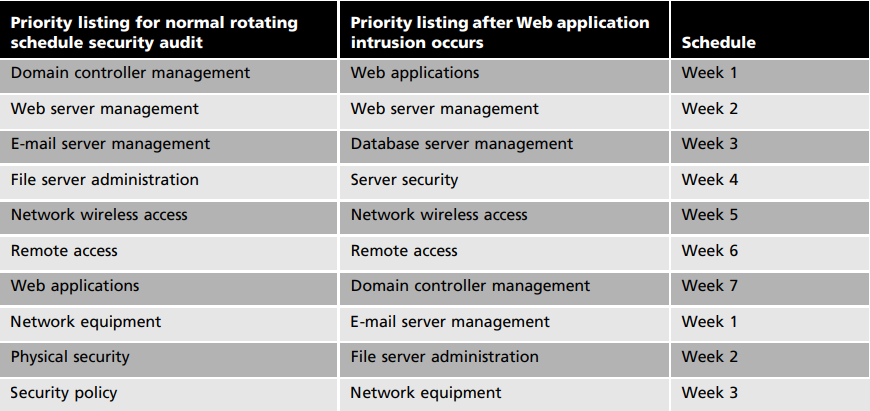
\includegraphics[width=0.8\textwidth]{assets/Schedule_audit}
    \caption{Пример графика проведения аудита}
\end{figure}

\paragraph{2. Аудит.}

На этом этапе подробный план аудита безопасности, составленный на предыдущем этапе, приводится в действие. Конкретные действия во время проведения аудита зависят от множества факторов, включая тип аудита, область аудита и организацию. Очевидно, что аудит, предназначенный для проверки физической безопасности, будет включать в себя совершенно иные действия, чем аудит, предназначенный для проверки администрирования СУБД. На Рис.2 в таблице показан список действий, которые обычно выполняются в процессе аудита для разных типов систем.

\begin{figure}[h!]
    \centering
    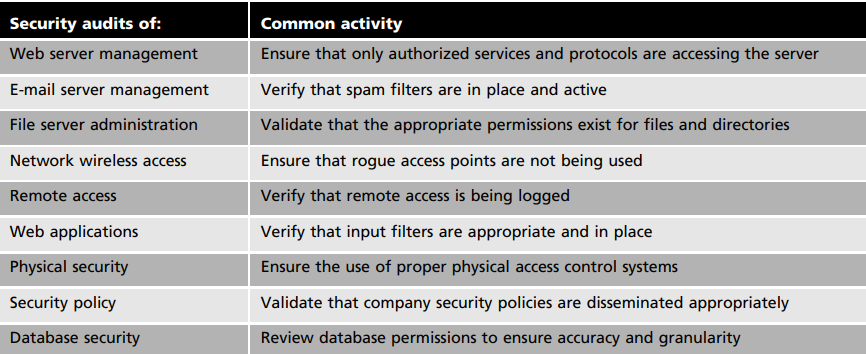
\includegraphics[width=0.8\textwidth]{assets/Common_actions_audit}
    \caption{Пример обычных действий при проведении аудита}
\end{figure}

\paragraph{3. Отчет.}

Заключительным этапом процесса аудита безопасности является подведение итогов, на котором аудитор или комитет аудиторов устно и письменно сообщает о результатах аудита.

Во всех аудиторских отчетах можно обнаружить некоторые важные общие черты, включающие исходную информацию, определенную область аудита, план и цель аудита, ключевые выводы, используемую для риск-аналитики методологию, рекомендации по устранению найденных уязвимостей.

\subsubsection{Процесс проведения аудита БД}

\paragraph{Подготовка и планирование аудита БД.}

Подготовка к аудиту безопасности БД требует, чтобы аудитор собрал как можно больше информации об инфраструктуре БД для четкого определения периметра аудита. Периметр должен включать подробную информацию о людях, данных, технологиях и документах, которые будут играть роль в рамках конкретного аудита. На Рис. 3 представлен пример периметра аудита БД.

Сбор информации включает в себя консультацию с администраторами БД, изучение схем баз данных, архитектуру сети, политик и процедур, связанных с БД. Часто организации имеют несколько СУБД, поэтому необходимо принять решение, сколько систем будет проверяться.

\begin{figure}[h!]
    \centering
    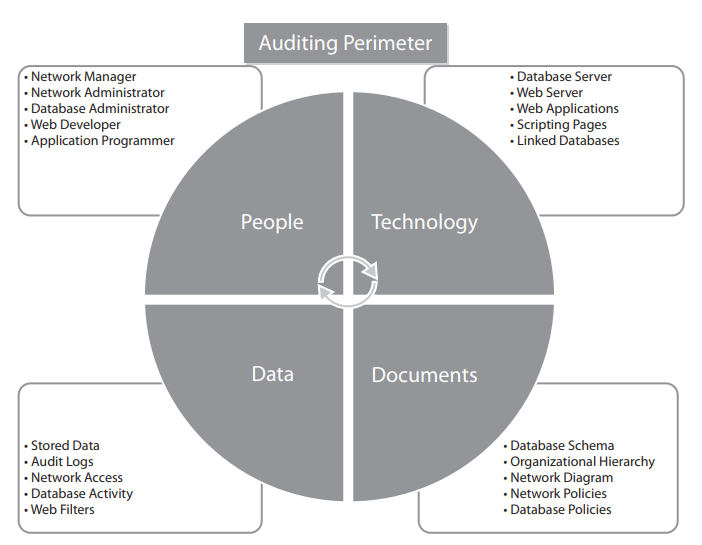
\includegraphics[width=0.8\textwidth]{assets/DB_audit_perimeter}
    \caption{Пример периметра аудита БД}
\end{figure}

На этом этапе также необходимо получить понимание функциональности, назначения и структуры всех используемых СУБД. Важна такая информация, как вендор СУБД, ОС функционирования СУБД, стратегия резервного копирования. Необходимо провести анализ данных на предмет связи с организационной иерархией, чтобы понять потребности сотрудников в хранении данных и манипулировании ими.

Анализ рисков и угроз является еще одним важным этапом планирования аудита БД, поскольку он помогает определить приоритетный список действий, который можно использовать в качестве отправной точки для аудита. Чтобы гарантировать, что были приняты все меры для защиты БД и учтены все риски, необходимо рассматривать всю инфраструктуру БД, в том числе сетевую.

Аудит БД может выполняться одним из двух способов. Аудитор может сначала сосредоточиться на компонентах, связанных с БД (например, веб-приложениях, веб-серверах, middleware, скриптах), прежде чем переходить к БД, или аудит может начаться с БД, и впоследствии проводится проверка связанных компонентов.

\paragraph{Аудит БД.}

Из-за большого количества ресурсов, необходимых для проверки всей инфрастуктуры БД, аудит обычно проводится частями, фокусируясь на конкретных функциях или компонентах. Эти части могут включать обслуживание серверов, администрирование учетных записей, контроль доступа, привилегии доступа к данным, пароли, шифрование, активность пользователей.

\paragraph{Обслуживание серверов.}

Аудит обслуживания сервера включает проверку стратегий резервного копирования, контроля обновлений и версий ПО, управления ресурсами и обновлениями оборудования. Ниже приведен список примеров аудиторских проверок:

\begin{enumerate}
	\item Установлены последние патчи безопасности СУБД
	\item Установлены последние критические обновления СУБД
	\item Используемая версия СУБД поддерживается
	\item Существует и используется процедура обновления СУБД
	\item Существует и применяется политика резервного копирования, включающая аварийное восстановление
	\item Существует и используется процедура проверки резервных копий
\end{enumerate}

\paragraph{Администрирование учетных записей.}

Аудит администрирования учетных записей включает проверку того, как администратор управляет учетными записями пользователей, а именно: создание, удаление учетных записей пользователей; применение политик безопасности; назначение групп, ролей и привилегий. Примеры аудиторских проверок:

\begin{enumerate}
	\item Различные роли администраторов четко определены
	\item Учетные записи администраторов распределяются согласно политике
	\item Неактивные или ненужные учетные записи пользователей удаляются
	\item Общие учетные записи не используются
	\item Учетные записи по умолчанию отключены или удалены
\end{enumerate}

\paragraph{Контроль доступа.}

Контроль доступа включает отслеживание доступа пользователей к БД. Контроль доступа необходим для обеспечения конфиденциальности, целостности и доступности СУБД. Примеры аудиторских проверок:

\begin{enumerate}
	\item Только доверенные IP-адреса могут получить доступ к базе данных
	\item Доступ к конфиденциальным данным имеют только те, кому они необходимы
	\item Администраторы не имеют возможности удаленно вносить изменения в БД без дополнительной аутентификации
	\item Доступ к резервным копиям и аварийному восстановлению разрешен только администраторам
\end{enumerate}

\paragraph{Привилегии доступа к данным.}

Обеспечение соответствия привилегий доступа во время аудита — трудоемкая задача, которая требует сотрудничества с сетевым администратором. Примеры аудиторских проверок:

\begin{enumerate}
	\item PUBLIC удален из системы
	\item Неявное предоставление привилегий тщательно рассматривается
	\item Используется принцип наименьших привилегий
	\item Привилегии учетной записи в операционной системе ограничены
\end{enumerate}

\paragraph{Пароли.}

Надежные пароли имеют решающее значение в доверенной среде, поскольку они представляют собой первую линию защиты, с которой столкнутся злоумышленники. Большинство СУБД можно настроить так, чтобы пароли автоматически соответствовали определенной политике. Аудит управления паролями включает проверку написанной политики, конфигурации сервера и учетных записей пользователей по умолчанию. Примеры аудиторских проверок:

\begin{enumerate}
	\item Опции управления паролями включены в СУБД
	\item Парольная политика включает спецификации для неудачных входов в систему, устаревания, сложности, истории, срока действия и содержимого
	\item Пароли по умолчанию должны быть изменены
	\item По возможности пароли не хранятся в БД
	\item Пароли шифруются с использованием стойкого шифрования, если они хранятся в БД
\end{enumerate}

\paragraph{Шифрование.}

Шифрование должно быть проверено как для хранящихся, так и для перемещаемых данных по БД. Примеры аудиторских проверок:

\begin{enumerate}
	\item Перемещаемые данные шифруются с использованием надежных методов шифрования
	\item Для шифрования данных используются симметричные ключи
	\item Шифрование настроено точно согласно политике
\end{enumerate}

\paragraph{Активность пользователей.}

Должен быть настроен мониторинг действий пользователей, работающих с СУБД. Примеры аудиторских проверок:

\begin{enumerate}
	\item Неудачные входы отслеживаются
	\item Неудачные запросы отслеживаются
	\item Изменения метаданных отслеживаются
\end{enumerate}

\paragraph{Отчет об аудите БД.}

Подготовка и презентация отчета об аудите БД совпадает с описанным ранее общим этапом аудита безопасности.

\begin{figure}[b]
Данный подразрадел является переводом и резюме 9 главы книги Database Security Альфред Баста и Мелисса Згола 2011 \href{https://pdfcoffee.com/alfred-basta-melissa-zgola-database-security-cengage-learning-2011-pdf-pdf-free.html}{ссылка на pdf}
\end{figure}

\clearpage

\subsection{Многоуровневая защита}
Уже было сказано про уровни в связке сеть-ОС-БД [\ref{pon:urovs}] и уровни ФСТЭК-а [\ref{pon:bez}].

Анализ наиболее успешных решений в области обеспе­чения информационной безопасности баз данных позволил сформулировать несколько полезных принципов, которыми можно руководствоваться при проектировании систем защиты \autocite{Smirnov2007}:
\begin{itemize}
	\item экономическая оправданность механизмов защиты
	\item открытое проектирование
	\item распределение полномочий между различными субъектами в соответствии с правилами организации
	\item минимально возможные привилегии для пользователей и администраторов
	\item управляемость системы при возникновении отказов и сбоев
	\item психологическая приемлемость работы средств защиты данных
\end{itemize}

Многоуровневую модель защиты данных может реализовать мандатный (заметим, что есть также дискреционная и ролевая модель безопасности) принцип построения системы разграничения доступа в СУБД.

Ключевые аспекты мандатного подхода к разграничению доступа, включая следующие принципы:
\begin{itemize}
	\item каждый субъект и объект должны быть четко идентифицированы
	\item существует упорядоченный набор меток конфиденциальности и соответствующих им уровней доступа, начиная от общедоступных объектов до наиболее конфиденциальных
	\item каждому объекту присваивается метка конфиденциальности, а каждому субъекту – степень доступа
	\item доступ к чтению информации из объекта разрешается только субъекту, чья степень доступа не ниже метки конфиденциальности объекта
	\item доступ к записи информации в объект разрешается только субъекту, чья метка конфиденциальности не выше метки объекта. Это также означает, что информация, записанная субъектом, автоматически получает уровень классификации субъекта
	\item в течение своего существования каждый субъект имеет уровень конфиденциальности, равный максимальной метке конфиденциальности объектов, к которым он имеет доступ
\end{itemize}

К преимуществам мандатного разграничения доступа включают более высокую надежность работы системы и большую простоту определения правил доступа по сравнению с дискреционным разграничением.

\subsection{Типы контроля безопасности: потоковый, контроль вывода, контроль доступа}
Про все три типа мы уже поговорили. В частности \ref{pon:pot} и \ref{pon:bez}. Единственное, что осталось уточнить -- это контроль доступа. 

Управление доступом представляет собой стратегию обеспечения безопасности информации, осуществляемую через контроль и регулирование использования ресурсов системы, таких как элементы базы данных, программное обеспечение и технические средства. Эта стратегия включает следующие ключевые функции защиты \autocite[с. 36]{Skakun}:
\begin{enumerate}
	\item идентификация пользователей и ресурсов системы
	\item проверка подлинности объекта или субъекта на основе предъявленного идентификатора (аутентификация)
	\item ограничение доступа и проверка полномочий (авторизация), обеспечивающие соблюдение установленных регламентов
	\item фиксация обращений к защищаемым ресурсам (протоколирование и аудит)
	\item реакция на попытки несанкционированного доступа
\end{enumerate}
То есть, идейно он этот вопрос распадается на два: \textit{кому} и \textbf{что} мы будем разрешать?

\paragraph{Кому?}

Получение доступа к ресурсам информационной системы предусматривает выполнение трех процедур: идентификации, аутентификации и авторизации.

Общепринято, что технологии идентификации и аутентификации являются обязательным элементом защищенных систем, так как обеспечивают аксиоматический принцип персонализации субъектов и, тем самым, реализуют первый (исходный) программ­но-технический рубеж защиты информации в компьютерных системах.

\begin{enumerate}
	\item Сущность процедуры идентификации состоит в назначении пользователю, т. е. объекту -- потребителю ресурсов сервера баз данных -- имени. Имя пользователя -- это некоторая уникальная метка, соответствующая принятым соглашениям именования и обеспечивающая однозначную идентификацию объекта реального мира в пространстве отображаемых объектов. С позиций ИС источники, предъявившие идентификатор, неразличимы.
	\item Сущность процедуры аутентификации состоит в подтверждении подлинности пользователя, представившего идентификатор.
	\item Сущность процедуры авторизации состоит в определении перечня конкретных информационных ресурсов, с которыми аутентифицированному пользователю разрешена работа.

\end{enumerate}
Процедуры идентификации, аутентификации и авторизации являются обязательными для любой защищенной ИС.

\paragraph{Что?}
Обычно используют одну из трех моделей безопасности: дискреционная, мандатная и ролевая.
\begin{enumerate}
	\item Простейшая (одноуровневая) модель безопасности данных строится на основе дискреционного (избирательного) принципа разграничения доступа, при котором доступ к объектам осуществляется на основе множества разрешенных отношений доступа в виде троек -- <<субъект доступа -- тип доступа -- объект доступа>>.

	Наглядным и распространенным способом формализованного представления дискреционного доступа является матрица доступа, устанавливающая перечень пользователей (субъектов) и перечень разрешенных операций (процессов) по отношению к каждому объекту базы данных (таблицы, запросы, формы, отчеты).

	\item Мандатная модель доступа характерна для случая, когда возможность конкретных действий с данными или документами определяется внешним, обычно глобальным собственником информации. Исторически в роли такого глобального собственника чаще всего выступало государство. Основная идея мандатной модели доступа состоит в приписывании объектам и субъектам доступа меток. Если метки объекта и субъекта соответствуют (в некотором смысле), то субъект получает право на выполнение определенных действий с объектом. В роли метки, приписываемой субъектам в государственных структурах, выступает, например, форма допуска. В реляционной модели в качестве структуры, обладающей меткой, естественно выбрать кортеж.

	\item В основу ролевой модели положена идея принадлежности всех данных системы некоторой организации, а не пользователю, как в случае моделей дискреционного и мандатного доступа. В целом модель ориентирована на упрощение и обеспечение формальной ясности в технологии обеспечения политики безопасности системы. Управление доступом в ролевой модели осуществляется как на основе матрицы прав доступа для ролей, так и с помощью правил, регламентирующих назначение ролей пользователям и их
	активацию во время сеансов.

	В ролевой модели классическое понятие субъект разделяется на две части: пользователь и роль. Пользователь — это человек, работающий с системой и выполняющий определенные служебные обязанности. Роль -- это активно действующая в системе абстрактная сущность, с которой связан ограниченный, логически связанный набор привилегий, необходимых для осуществления определенной деятельности. (Самым распространенным примером роли явля­ется присутствующая почти в каждой системе учетная запись администратора (например, root для UNIX и Administrator для Windows), который обладает специальными полномочиями и может использоваться несколькими пользователями.

	Ролевая модель включает три компонента: модель отображения пользователь -- роль, модель отображения привилегия -- роль и модель отображения роль -- роль. Для упрощения логической структуры объектов управления вводится понятие иерархии ролей. Роль, входящая в иерархию, может включать другие роли, наследуя все привилегии включаемых
	ролей.
\end{enumerate}
\clearpage

\section{Теоретические основы безопасности в СУБД}

\subsection{Критерии защищенности БД}

\paragraph{Критерии оценки надежных компьютерных систем (TCSEC)}
\paragraph{Понятие политики безопасности}
\paragraph{Совместное применение различных политик безопасности в рамках единой модели}
\paragraph{Интерпретация TCSEC для надежных СУБД (TDI)}
\paragraph{Оценка надежности СУБД как компоненты вычислительной системы}
\paragraph{Монитор ссылок}
\paragraph{Применение TCSEC к СУБД непосредственно}
\paragraph{Элементы СУБД, к которым применяются TDI: метки, аудит, архитектура системы, спецификация, верификация, проектная документация}
\paragraph{Критерии безопасности ГТК}

\subsection{Модели безопасности в СУБД}

\paragraph{Дискреционная (избирательная) и мандатная (полномочная) модели безопасности}
\paragraph{Классификация моделей}
\paragraph{Аспекты исследования моделей безопасности}
\paragraph{Особенности применения моделей безопасности в СУБД}
\paragraph{Дискреционные модели: HRU, Take-Grant, Action-Entity, Wood}
\paragraph{Мандатные модели: Bell-LaPadula, Biba, Dion, Sea View, Jajodia\&Sandhu, Smith\&Winslett, решеточная}
\paragraph{БД с многоуровневой секретностью (MLS)}
\paragraph{Многозначность}
\section{Механизмы обеспечения целостности СУБД}

\subsection{Угрозы целостности СУБД}
Задача обеспечения целостности предусматривает комплекс мер по предотвращению непреднамеренного изменения или уничтожения информации, используемой информационной системой управления или системой поддержки принятия решений. Изменение или уничтожение данных может быть следствием неблагоприятного стечения обстоятельств и состояния внешней среды (стихийные бедствия, пожары и т. п.), неадекватных действий пользователей (ошибки при вводе данных, ошибки операторов и т. п.) и проблем, возникающих при многопользовательской обработке данных \autocite{Lihonosov2011}.


Например, с помощью SQL-операторов UPDATE, INSERT и DELETE можно изменить данные в СУБД. Опасность заключается в том, что пользователь, обладающий соответствующими привилегиями, может модифицировать все записи в таблице \autocite{Utebov2008}.

\paragraph{Основные виды и причины возникновения угроз целостности} ~\\

Нарушение целостности информационной базы может произойти по причинам, по которым может произойти и нарушение доступности информации.
Перечислим основные угрозы целостности информации \autocite{Pirogov2009}:

\begin{enumerate}
\item \textbf{Внутренние угрозы целостности ИС}.
    \begin{itemize}
        \item Случайное или умышленное отступление от правил эксплуатации. Например, правила могут предусматривать определенный набор параметров сервера (объем памяти, производительность процессора, объем дискового пространства, версия операционной системы и т.п.), на котором предполагается использовать ИС;
        \item Выход системы из штатного режима эксплуатации в силу случайных или преднамеренных действий пользователей, администраторов и т.д.;
        \item Ошибки конфигурирования системы. В сложных системах конфигурирование выполняется при установке и настройке системы;
        \item Отказ программного обеспечения. Программное обеспечение может содержать ошибки, в том числе и такие, которые могут привести к серьезным повреждениям данных. Кроме этого преднамеренно может быть изменен алгоритм программы. Таким образом, следует защищать программное обеспечение информационной системы и от случайного повреждения, и от исправления непосредственно исполняемых модулей.
    \end{itemize}

\item \textbf{Внешние угрозы целостности ИС}.
    \begin{itemize}
        \item Нарушение условий работы ИС (проблемы с системами связи, отключения электропитания, отопления и т.п.).
        \item Разрушение или повреждение помещений, связанное с природными катаклизмами. Конечно, такая ситуация на первый взгляд кажется мало возможной, но это вполне вероятно в регионах, например, с сейсмической неустойчивостью.
        \item Разрушение информации намеренными действиями человека (диверсия). В данном случае речь идет о действиях людей, не являющихся обслуживающим персоналом данной системы.
        \item Сетевые атаки, вирусные программы и другое вредоносное программное обеспечение.
    \end{itemize}
\end{enumerate}

\paragraph{Способы противодействия} ~\\

Основными средствами защиты целостности информации в ИС являются \autocite{Pirogov2009}:
\begin{itemize}
    \item Транзакционные механизмы, позволяющие восстановить целостность данных в случае незначительных сбоев, ACID-свойства. \autocite{worksol1, DBtest};
    \item Контроль целостности на уровне базы данных. Реализация CHECK, FOREIGN KEY, NOT NULL и триггеров, предтовращающих некорректное изменение данных. \autocite{flenovinfo};
    \item Использование WAL (Write-Ahead Logging) - позволят сохранить изменение перед его внесением в основную базу. То есть проще сделать откат транзакции и восстановление данных. \autocite{WALintro};
    \item Резервное копирование данных. Использование PITR (point-in-time recovery), географически распределеная репликация на случай какого-то серьезного сбоя, \autocite{PITRintro};
    \item Периодическое тестирование системы на предмет нарушения целостности, анализ логов БД, а также использование IDS с целью попыток выявления попыток несанкционированного изменения данных \autocite{DBtest}.
    \item Использование отказоустойчивых серверов, UPS (системы бесперебойного питания), аппаратных средств шифрования, осуществление контроля доступа к серверному оборудованию \autocite{tolerance1, tolerance2}.
\end{itemize}

\subsection{Метаданные и словарь данных}

\begin{grayquote}
	\textbf{Метаданные} -- Это данные, описывающие другие данные. Это важный элемент хранилища данных, который предоставляет возможность показывать пользователю предметно-ориентированную структуру, а не набор абстрактно-связанных таблиц. Метаданные предназначены для хранения информации о происхождении данных, о любых изменениях данных, о расположении данных, об ограничениях на данные, о соответствии данных тем или иным объектам предметной области и т. д. \autocite{Pirogov2009}
\end{grayquote}

Говоря более простым языком: 
Если \textbf{данные} — то, что хранится в базе данных приложения (данные о клиентах, пользователях, заказах и т.п.), то \textbf{метаданные} — это описание структуры данных. Описание того, какие типы объектов хранятся в базе данных, какие у них есть поля (атрибуты, элементы), описание зависимостей между объектами. В общем случает типы могут наследовать атрибуты родительского типа, а один атрибут в общем случае может присутствовать у двух и более типов, несвязанных отношением наследования \autocite{Metadatahabr}.

\paragraph{Назначение словаря данных} ~\\

Согласно реляционной модели данных, информация о структуре базы данных должна храниться в самой базе данных, в виде специальных таблиц. Это требование описано в 4-м правиле Кодда (Dynamic On-Line Catalog Based on the Relational Model), согласно которому СУБД должна автоматически управлять метаданными и обеспечивать их доступность через стандартные средства запросов.

Для организации хранения метаданных в реляционных СУБД используются системные каталоги, которые также называют "словари данных".

\begin{grayquote}
    \textbf{Системный каталог} — это совокупность специальных таблиц, автоматически создаваемых и управляемых самой СУБД. Он содержит информацию о структуре базы данных, включая перечень таблиц, индексов, ограничений целостности, а также сведения о пользователях, их привилегиях и других параметрах системы \autocite{IntuitLec14}.
\end{grayquote}

Системные каталоги со временем развивались. Первые реализации каталогов появились еще в 1970-х годах в исследовательских проектах \textbf{IBM System R} и \textbf{Ingres}, но формально описание системного каталога было включено в стандарт \textbf{SQL-86}. В нем задавались базовые требования к хранению метаданных, но без единого формата их представления \autocite{DictHist}.

В \textbf{SQL-92} была стандартизирована структура системного каталога, а точнее представления, объединенные в схему \texttt{INFORMATION\_SCHEMA}. Эта штука в какой-то степени развязала руки разработчикам писать универсальные запросы для получения информации о таблицах, индексах, ограничениях и других объектах БД вне зависимости от конкретной СУБД. Однако на момент принятия стандарта, многие СУБД уже использовали собственные форматы каталогов, и их переход на \texttt{INFORMATION\_SCHEMA} оказался затруднительным.

\paragraph{Реализация системных каталогов в разных СУБД}

Реализация и организация системных каталогов отличаются в зависимости от СУБД.

\begin{enumerate}
    \item \textbf{PostgreSQL}. \autocite{PostgreSQLdocc51,HabrDataOrgp1,YTcoursepostgre}
    
    В PostgreSQL системный каталог — это набор таблиц и представлений, содержащих метаданные обо всех объектах базы данных. Эти таблицы расположены в схеме \texttt{pg\_catalog}, которая по умолчанию включена в путь поиска. То есть можно обращаться к таблицам без явного указания схемы. Примеры таких таблиц: \texttt{pg\_class} (информация о таблицах и представлениях), \texttt{pg\_attribute} (сведения о столбцах) и \texttt{pg\_index} (данные об индексах). \autocite{PostgreSQLdocc51}

    Хотя системные каталоги и являются обычными таблицами, их прямое изменение не рекомендуется, так как это может привести к некорректной работе системы. Для внесения изменений рекомендуется использовать соответствующие SQL-команды, такие как \texttt{CREATE TABLE}, которая автоматически обновляет соответствующие записи в системном каталоге.

    Для получения информации из системного каталога рекомендуется использовать стандартные представления, наподобие \texttt{information\_schema}.

    Подробную информацию о системных каталогах PostgreSQL можно найти в официальной документации. \autocite{PostgreSQLdocc51}

    \item \textbf{MySQL}.
    
    В MySQL метаданные о базах данных и их объектах хранятся в специальной базе данных под названием \texttt{information\_schema}. Эта база данных содержит набор представлений, предоставляющих информацию о структурах баз данных (таблицах, столбцах, индексах, привилегиях пользователей).

    Например, представление \texttt{TABLES} в \texttt{information\_schema} содержит информацию обо всех таблицах, их имена, типы и используемые механизмы хранения. Представление \texttt{COLUMNS} дает сведения о столбцах таблиц (имена, типы данных и дополнительные характеристики).

    Доступ к данным в \texttt{information\_schema} осуществляется с помощью стандартных SQL-запросов. Например, получить список всех таблиц в определенной базе данных можно следующим запросом:

    \begin{lstlisting}[language=SQL]
    SELECT table_name
    FROM information_schema.tables
    WHERE table_schema = 'DATABASE_NAME';
    \end{lstlisting}

    Подробную информацию о структуре и содержимом \texttt{information\_schema} можно найти в официальной документации MySQL. \autocite{Mysqldoc1}
    
    Также стоит отметить, что в MySQL физическое хранение данных организовано в виде файловой системы, где каждая база данных представлена как подкаталог в основном каталоге данных сервера. Внутри каждого подкаталога файлы соответствуют таблицам и другим объектам базы данных. \autocite{IntuitMySQLadm}

    \item \textbf{Microsoft SQL Server}. \autocite{MicrosoftLearnSQLserver,professorweb,HabrTsql}

    В Microsoft SQL Server метаданные обо всех объектах базы данных хранятся в системных представлениях каталога, расположенных в схеме \texttt{sys}. Информация этих представлений содержит данные о таблицах, представлениях, столбцах, индексах, ограничениях и прочих объектах БД. Использование системных представлений позволяет администраторам и разработчикам получать структурированную информацию о состоянии БД и её объектах.
    
    \subparagraph{Основные представления каталога}
    
    Примеры наиболее часто используемых представлений:
    
    \begin{itemize}
        \item \texttt{sys.tables} — информация о всех таблицах в БД (имена, идентификаторы, даты создания);
        \item \texttt{sys.columns} — сведения о столбцах таблиц (имена, типы данных, порядковые номера);
        \item \texttt{sys.indexes} — информация об индексах (типы индексов, их назначение);
        \item \texttt{sys.foreign\_keys} — сведения о внешних ключах (ограничения ссылочной целостности);
        \item \texttt{sys.database\_principals} — информация о пользователях БД.
    \end{itemize}
    
    \subparagraph{Примеры запросов к системным представлениям}
    
    Для получения списка всех таблиц в текущей БД используется SQL-запрос:
    
    \begin{lstlisting}[language=SQL]
    SELECT name 
    FROM sys.tables;
    \end{lstlisting}
    
    Если необходимо получить список всех столбцов конкретной таблицы:
    
    \begin{lstlisting}[language=SQL]
    SELECT column_name, data_type, is_nullable
    FROM information_schema.columns
    WHERE table_name = 'Employees';
    \end{lstlisting}
    
    Для просмотра индексов таблицы:
    
    \begin{lstlisting}[language=SQL]
    SELECT i.name AS IndexName, t.name AS TableName
    FROM sys.indexes i
    JOIN sys.tables t ON i.object_id = t.object_id
    WHERE t.name = 'Employees';
    \end{lstlisting}
    
    \subparagraph{Рекомендации по использованию}
    
    Рекомендуется использовать системные представления каталога вместо прямого доступа к системным таблицам, так как представления:
    
    \begin{itemize}
        \item предоставляют стандартизированный интерфейс для получения метаданных;
        \item обеспечивают обратную совместимость при обновлении версий SQL Server;
        \item позволяют получать данные в удобном формате без необходимости разбираться во внутренней структуре системы.
    \end{itemize}

    \item \textbf{Oracle}.
    В Oracle Database словарь данных состоит из нескольких наборов представлений. Во многих случаях такой набор состоит из трех представлений, содержащих аналогичную информацию и отличающихся друг от друга своими префиксами \autocite{Kirillov2009}.\\

    Словарь данных базы данных Oracle имеет два основных применения:
    \begin{itemize}
        \item Oracle обращается к словарю данных каждый раз, когда выполняются команды языка DDL (Data Definition Language), например \texttt{CREATE TABLE}, \texttt{ALTER TABLE}, \texttt{DROP TABLE} и тд. Например, при создании таблицы Oracle вносить соответвсуюшую запись в \texttt{DBA\_TABLES} и \texttt{ALL\_TABLES}.
        \item каждый пользователь Oracle может обращаться к словарю данных как к справочнику со сведениями по базе данных (доступные объекты). Нпример DBA может юзать словарь данныхх для мониторинга структуры схемы или например анализа привилегий юзеров
    \end{itemize}

    При этом словарь данных всегда доступен при открытой базе данных. Он размещается в табличном пространстве SYSTEM, которое всегда находится в состоянии Online, когда база данных открыта.

    Основные категории представлений \autocite{oracledbdoc1}:
    \begin{enumerate}

        \item \textbf{Представления с префиксом \texttt{USER\_}} содержат информацию об объектах, принадлежащих текущему пользователю. Напирмер \texttt{USER\_TABLES} отображает таблицы, созданные текущим пользователем, а \texttt{USER\_TAB\_COLUMNS} даст инфу о столбцах тааблиц пользователя.
        Пример запроса:
        \begin{lstlisting}[language=SQL]
        SELECT table_name 
        FROM user_tables;
        \end{lstlisting}

        \item \textbf{Представления с префиксом \texttt{ALL\_}} предоставляют информацию обо всех объектах, к которым текущий пользователь имеет доступ, независимо от владельца. Например \texttt{ALL\_TABLES} показывает все таблицы, доступные пользователю. \texttt{ALL\_TAB\_COLUMNS} показывает информацию о столбцах всех доступнх таблиц.
        Пример запроса:
        \begin{lstlisting}[language=SQL]
        SELECT table_name 
        FROM all_tables 
        WHERE owner = 'HR';
        \end{lstlisting}

        \item \textbf{Представления с префиксом \texttt{DBA\_}} содержат информацию обо всех объектах в БД и доступны только пользователям с соответствующими привилегиями (типа админ). К примеру \texttt{DBA\_TABLES} предоставляет список всех таблиц в БД, \texttt{DBA\_USERS} - информациб обо всех пользователях БД.
        Пример запроса:
        \begin{lstlisting}[language=SQL]
        SELECT username 
        FROM dba_users;
        \end{lstlisting}

    \end{enumerate}

    Столбцы в представленях с префиксами \texttt{USER\_}, \texttt{ALL\_}, \texttt{DBA\_} идентичны, но есть нюанс. Объем данных возвращаемых каждый представлением зависит от прав доступа пользователя. В представлениях \texttt{USER\_} к примеру обычно нет столбца \texttt{OWNER}, так как подразумевается что владелец это текущий пользователь, выдавший запрос. Некоторые представления DBA имеют дополнительные столбцы, которые содержат информацию, полезную для БД.

    \textbf{Динамические представления происзводительности \texttt{V\textdollar}}. \autocite{oracledbdoc2}

    Помимо статических представлений словаря данных, Oracle предоставляет Dynamic Performance Views, также извесные как \texttt{V\textdollar}-представления. Они содержат информацию о текущем состоянии БД и её производительности. Они обновляются в реальном времени и позволяют отслеживать активность системы, типа там текущие сессии, параметры, статистику производительности и тд. То есть используются они для мониторинга активности БД в рельном времени.

    Как пример можно привести \texttt{V\textdollar SESSION} (информация о текущих подключенных сессиях) или \texttt{V\textdollar PARAMETER} (текущие параметры конфигурации БД).

    Пример запроса:
    \begin{lstlisting}[language=SQL]
    SELECT sid, serial#, username, status 
    FROM v$session 
    WHERE status = 'ACTIVE';
    \end{lstlisting}
    
\end{enumerate}

\paragraph{Типы словарей данных} ~\\

Существует два типа словарей данных. Активные и пассивные, они отличаются уровнем автоматической синхронизации \autocite{DataDictionary}:

\begin{grayquote}
    \textbf{Активные словари данных} -- словари данных, созданные в описываемых ими базах данных, которые автоматически отражают любые изменения внутри этих баз, что позволяет избежать любых несоответствий между словарями данных и описываемыми данными.
\end{grayquote}

\begin{grayquote}
    \textbf{Словари пассивных данных} -- словари данных, созданные как отдельные от описываемых ими баз данных сущности. Они требуют дополнительной логики для синхронизации с базами данных, которые они описывают.
\end{grayquote}

\paragraph{Доступ к словарю данных} ~\\

По 4 правилу Кодда (Dynamic On-Line Catalog Based on the Relational Model) словарь данных должен сохраняться в форме реляционных таблиц, и СУБД должна поддерживать доступ к нему при помощи стандартных языковых средств.


Для доступа к словарю данных используются инструкции SQL. Так как словарь данных доступен только для чтения, допускается выполнять только запросы таблиц и представлений.

Можно запрашивать представления словаря, которые основаны на таблицах словаря, чтобы найти сведения, такие как \autocite{SqlOracle}:
\begin{itemize}
    \item Определения всех объектов схемы в словаре (таблицы, представления, индексы, синонимы, последовательности, процедуры, функции, пакеты, триггеры и так далее);
    \item Значения по умолчанию для столбцов;
    \item Сведения об ограничениях целостности;
    \item Имена пользователей Oracle;
    \item Привилегии и роли, предоставленные каждому пользователю;
    \item Другие общие сведения о базе данных.
\end{itemize}

\paragraph{Состав словаря} ~\\

В состав словаря данных базы данных могут входить \autocite{DataDictionary}:

\begin{itemize}
    \item Списки объектов данных (имена и определения);
    \item Свойства элемента данных (тип данных, уникальные идентификаторы, размер, допустимость значений NULL, индексы и параметр required);
    \item ERD-диаграммы 
        \footnote{Схема «сущность-связь» (также ERD или ER-диаграмма) — это разновидность блок-схемы, где показано, как разные «сущности» (люди, объекты, концепции и так далее) связаны между собой внутри системы.};
    \item Диаграммы системного уровня (они же DFD-диаграммы);
    \item Справочные данные — доступные пользователю представления, которые суммируют и отображают в удобном формате информацию из базовых таблиц словаря. Эти представления декодируют информацию базовых таблиц, представляя её в полезном виде, таком как имена пользователей или таблиц, чтобы добиться человекочитаемости данных. Большинство пользователей имеют доступ к этим представлениям вместо диаграмм системного уровня;
    \item Бизнес-логика (например, для проверки качества данных и объектов схемы);
\end{itemize}


\subsection{Понятие транзакции}

\begin{grayquote}
    Последовательность действий над данными, обрабатываемая СУБД как единая операция, будем называть \textbf{транзакцией}.
\end{grayquote}

Из определения ясно, что транзакция может состоять из одной или нескольких команд языка SQL. При этом команды языка SQL могут перемежаться командами, не выполняющими непосредственно операций над данными (не читающими данные, не изменяющими данные, не изменяющими структуру данных). Таким образом, в качестве транзакции может быть выбрана любая часть программы, содержащая команды чтения или записи данных. В частности, транзакция может состоять всего из одной команды, например INSERT, или из сотен команд, изменяющих или не изменяющих данные.


Понятие транзакции чрезвычайно емкое. Оно в действительности тесно связано с концептуальной моделью данных и всей информационной системы. Дело в том, что на уровне пользователя операции над данными носят предметный характер: начислить зарплату, уволить работника, перевести деньги на другой счет и т. п. Для выполнения таких операций часто необходимо выполнить десятки, и даже сотни команд языка SQL. Однако вся эта последовательность команд должна быть подчинена одной цели: операция уровня пользователя должна быть обязательно выполнена. Что будет, если при выполнении такой цепочки команд произойдет сбой? Как рассматривать тогда выполняемую операцию — как частично выполненную? Но как в дальнейшем система узнает, что операция была только частично выполнена, и как ее закончить? Все эти вопросы, в конце концов, и приводят к понятию \textbf{"транзакция"} \autocite{Pirogov2009}.


\paragraph{Фиксация транзакции} ~\\

Согласно требованиям ACID (Atomic, Consistent, Isolated, Durable) транзакция должна быть устойчивой. После своего завершения она сохраняется в системе, которую ничто не может вернуть в исходное (до начала транзакции) состояние, т. е. происходит фиксация транзакции, означающая, что ее действие постоянно даже при сбое системы. При выполнении отдельных операций транзакции могут быть нарушены какие-либо требования целостности данных (в первую очередь имеются в виду корпоративные правила целостности, см. главу 2). Однако по окончании выполнения транзакции (фиксация транзакции) все правила целостности базы данных будут соблюдены. \\


Согласно стандарту транзакция начинается с первой команды, которая обращается к данным. После этого транзакция продолжается до тех пор, пока не будет выполнена команда COMMIT WORK (или просто COMMIT) либо не будет закрыто соединение к базе данных. При выполнении команды COMMIT WORK происходит фиксация транзакции, другими словами, после этой команды откат транзакции уже будет невозможен \autocite{Pirogov2009}.


\paragraph{Прокрутки вперед и назад} ~\\

В результате сбоя СУБД могут возникнуть две потенциальные ситуации \autocite{Karpova2009}:

\begin{itemize}
    \item Блоки, содержащие подтверждённые модификации, не были записаны в файлы данных, так что эти изменения отражены лишь в журнале транзакций. Следовательно, журнал транзакций содержит подтверждённые данные, которые должны быть переписаны в файлы данных.
    \item Журнал транзакций и блоки данных содержат изменения, которые не были подтверждены. Изменения, внесенные неподтверждёнными транзакциями, во время восстановления БД должны быть удалены из файлов данных.
\end{itemize}

Для того чтобы разрешить эти ситуации, СУБД автоматически выполняет два этапа при восстановлении после сбоев: прокрутку вперед и прокрутку назад.

\begin{enumerate}
    \item Прокрутка вперед заключается в применении к файлам данных всех изменений, зарегистрированных в журнале транзакций. После прокрутки вперед файлы данных содержат все как подтверждённые, так и неподтверждённые изменения, которые были зарегистрированы в журнале транзакций.
    \item Прокрутка назад заключается в отмене всех изменений, которые не были подтверждены. Для этого используются журнал транзакций и сегменты отката, информация из которых позволяет определить и отменить те транзакции, которые не были подтверждены, хотя и попали на диск в файлы БД.
\end{enumerate}

После выполнения этих этапов восстановления БД находится в согласованном состоянии и с ней можно работать.

\paragraph{Контрольная точка} ~\\

Критическим моментом в отказе системы является потеря содержимого основной (оперативной) памяти (в частности, буферов базы данных). Поскольку точное состояние любой выполнявшейся в момент отказа системы транзакции остается неизвестным, такая транзакция не может быть успешно завершена. Поэтому при перезапуске системы любая такая транзакция будет отменена (т.е. будет выполнен ее откат). 


Более того, при перезапуске системы, возможно, потребуется повторно выполнить некоторые транзакции, которые были успешно завершены до аварийного останова, но выполненные ими обновления еще не были перенесены из буферов оперативной памяти в физическую базу данных во вторичной памяти.


Возникает очевидный вопрос: как система определяет в процессе перезапуска, какую транзакцию следует отменить, а какую выполнить повторно? Ответ заключается в том, что система автоматически создает контрольные точки с некоторым наперед заданным интервалом (обычно, когда в журнале накапливается определенное число записей). Для создания контрольной точки требуется \autocite{Date2005}:

\begin{enumerate}
    \item Выполнить принудительное сохранение содержимого буферов оперативной памяти в физической базе данных 
    \item Осуществить принудительное сохранение специальной записи контрольной точки в журнале на физическом носителе. Запись контрольной точки содержит список всех транзакций, выполняемых в тот момент, когда создавалась контрольная точка.
\end{enumerate}

\paragraph{Откат} ~\\

Для управления транзакциями в системах, поддерживающих механизм транзакций и язык SQL, используется оператор отката транзакции (отмены изменений): ROLLBACK [WORK]. Для фиксации или отката транзакции система создаёт неявные точки фиксации и отката. По команде rollback система откатит транзакцию на начало (на неявную точку отката).

Для обеспечения целостности транзакции СУБД может откладывать запись изменений в БД до момента успешного выполнения всех операций, входящих в транзакцию, и получения команды подтверждения транзакции (commit). Но чаще используется другой подход: система записывает изменения в БД, не дожидаясь завершения транзакции, а старые значения данных сохраняет на время выполнения транзакции в сегментах отката.

\textbf{Сегмент отката (Rollback Segment, RBS)} – это специальная область памяти на диске, в которую записывается информация обо всех текущих (незавершённых) изменениях. Обычно записывается "старое" и "новое" содержимое изменённых записей, чтобы можно было восстановить прежнее состояние БД при откате транзакции (по команде rollback) или при откате текущей операции (в случае возникновения ошибки). Данные в RBS хранятся до тех пор, пока транзакция, изменяющая эти данные, не будет завершена. Потом они могут быть перезаписаны данными более поздних транзакций.


Команда savepoint запоминает промежуточную "текущую копию" состояния базы данных для того, чтобы при необходимости можно было вернуться к состоянию БД в точке сохранения: откатить работу от текущего момента до точки сохранения (rollback to <имя\_точки>) или зафиксировать работу от начала транзакции до точки сохранения (commit to <имя\_точки>). На одну транзакцию может быть несколько точек сохранения (ограничение на их количество зависит от СУБД). Для сохранения сведений о транзакциях СУБД ведёт журнал транзакций. 

\textbf{Журнал транзакций} –- это часть БД, в которую поступают данные обо всех изменениях всех объектов БД. Журнал недоступен пользователям СУБД и поддерживается особо тщательно (иногда ведутся две копии журнала, хранимые на разных физических носителях). 

Форма записи в журнал изменений зависит от СУБД. Но обычно там фиксируется следующее:

\begin{itemize}
    \item Номер транзакции (номера присваиваются автоматически по возрастанию);
    \item Состояние транзакции (завершена фиксацией или откатом, не завершена, находится в состоянии ожидания);
    \item Точки сохранения (явные и неявные);
    \item Команды, составляющие транзакцию, и прочие
\end{itemize}

Начало транзакции соответствует появлению первого исполняемого SQLоператора. При этом в журнале появляется запись об этой транзакции \autocite{Karpova2009}.

\paragraph{Транзакции как средство изолированности пользователей} ~\\

Поддержание механизма транзакций —- показатель уровня развитости СУБД и основа обеспечения целостности базы данных. Транзакции также составляют основу изолированности в многопользовательских системах, где с одной базой данных параллельно могут работать несколько пользователей и (или) прикладных программ. 


Одна из основных задач СУБД —- обеспечение изолированности, т. е. создание такого режима функционирования, при котором каждому пользователю казалось бы, что база данных доступна только ему. Такую задачу СУБД принято называть параллелизмом транзакций. Большинство выполняемых действий производится в теле транзакций. По умолчанию каждая команда выполняется как самостоятельная транзакция. Как было показано ранее, при необходимости пользователь может явно указать ее начало и конец, чтобы иметь возможность включить в нее несколько команд.


Решение проблемы параллельной обработки базы данных заключается в том, что строки таблиц блокируются, а последующие транзакции, модифицирующие эти строки, отвергаются и переводятся в режим ожидания. В связи со свойством сохранения целостности базы данных транзакции являются подходящими единицами изолированности пользователей. Действительно, если каждый сеанс взаимодействия с базой данных реализуется транзакцией, то пользователь начинает с того, что обращается к согласованному состоянию базы данных — состоянию, в котором она могла бы находиться, даже если бы пользователь работал с ней в одиночку.


Если бы в СУБД не были реализованы механизмы блокирования, то при одновременном чтении и изменении одних и тех же данных несколькими пользователями могли бы возникнуть проблемы одновременного доступа.


\paragraph{Конфликты транзакций и уровни изоляции} ~\\

Уровни изоляции определяют степень, в которой транзакция должна быть изолирована от изменений данных, сделанных любой другой транзакцией в системе базы данных. Уровни изоляции отличаются разрешениями следующих конфликтов:

\begin{itemize}
    \item 
        \textbf{Потерянное обновление (Lost Update)} — когда несколько транзакций что-то обновили в БД, но по итогам результат такой, будто отработала лишь часть транзакций. Самый опасный побочный эффект, по сути, полное отсутствие изоляции транзакций — две транзакции читают одну ячейку, записывают изменённое значение (одна вычитает стоимость мороженого, другая плату за квартиру). В итоге в ячейке значение от второй транзакции, а первой как будто и не было.
    \item 
        \textbf{Грязное чтение (Dirty Read)} — ситуация, когда транзакция считывает данные, которые еще не были зафиксированы. Например, транзакция 1 обновляет строку и оставляет ее незафиксированной, в то время как транзакция 2 читает обновленную строку. Если транзакция 1 откатывает изменение, транзакция 2 будет считывать данные, которые считаются никогда не существовавшими.
    \item 
        \textbf{Неповторяемое чтение (Non-repeatable Read)} — когда транзакция дважды считывает одну и ту же строку и каждый раз получает другое значение. Например, предположим, что транзакция T1 считывает данные. Из-за параллелизма другая транзакция T2 обновляет те же данные и фиксирует их. Теперь, если транзакция T1 повторно считывает те же данные, она получит другое значение.
    \item 
        \textbf{Фантомное чтение (Phantom Reads)} — когда выполняются два одинаковых запроса, но извлекаемые ими строки различаются. Например, транзакция T1 извлекает набор строк, удовлетворяющих некоторым критериям поиска. Далее транзакция T2 создает несколько новых строк, соответствующих критериям поиска для транзакции T1. Если транзакция T1 повторно выполняет инструкцию, которая считывает строки, на этот раз она получает другой набор строк. Отличие от предыдущего пункта в том, что в этом случае происходит агрегация строк, а в предыдущем происходит чтение лишь одной строки.
\end{itemize}

Основываясь на политиках разрешения перечисленных конфликтов, стандарт SQL определяет четыре уровня изоляции:

\begin{itemize}
    \item 
        \textbf{Read Uncommitted} — это самый низкий уровень изоляции. На этом уровне одна транзакция может считывать еще не зафиксированные изменения, сделанные другими транзакциями, тем самым допуская грязное чтение. На этом уровне транзакции не изолированы друг от друга.
    \item 
        \textbf{Read Committed} — уровень изоляции гарантирует, что любые считанные данные фиксируются в момент их чтения. Таким образом, он не допускает грязного чтения. Транзакция удерживает блокировку чтения или записи для текущей строки и, таким образом, предотвращает ее чтение, обновление или удаление другими транзакциями.
    \item 
        \textbf{Repeatable Read} — транзакция удерживает блокировки чтения для всех строк, на которые она ссылается, и записывает блокировки для указанных строк для действий обновления и удаления. Поскольку другие транзакции не могут читать, обновлять или удалять эти строки, следовательно, это позволяет избежать неповторяющегося чтения.
    \item 
        \textbf{Serializable} — самый высокий уровень изоляции. Выполнение определяется как выполнение операций, в которых одновременно выполняемые транзакции кажутся последовательно выполняемыми \autocite{BeginningSQL}.
\end{itemize}

\begin{table}[h]
\begin{tabularx}{\textwidth}{|X|X|X|X|X|}
    \hline
                     & Фантомное чтение         & Неповторяющееся чтение   & Грязное чтение           & Потерянное обновление    \\ \hline
    Serializable     & \cellcolor[HTML]{32CB00} & \cellcolor[HTML]{32CB00} & \cellcolor[HTML]{32CB00} & \cellcolor[HTML]{32CB00} \\ \hline
    Repeatable Read  & \cellcolor[HTML]{FE0000} & \cellcolor[HTML]{32CB00} & \cellcolor[HTML]{32CB00} & \cellcolor[HTML]{32CB00} \\ \hline
    Read Committed   & \cellcolor[HTML]{FE0000} & \cellcolor[HTML]{FE0000} & \cellcolor[HTML]{32CB00} & \cellcolor[HTML]{32CB00} \\ \hline
    Read Uncommitted & \cellcolor[HTML]{FE0000} & \cellcolor[HTML]{FE0000} & \cellcolor[HTML]{FE0000} & \cellcolor[HTML]{32CB00} \\ \hline
\end{tabularx}
\caption{Уровни изоляции транзакций}
\end{table}


\paragraph{Методы сериализации транзакций} ~\\

Делятся на три типа:

\begin{itemize}
    \item 
        \textbf{С блокирующим планировщиком (Blocking Sheduler)} — для каждого запроса планировщик запрашивает блокировку. Каждая блокировка запрашивается в определенном режиме (чтение или запись). Если запрашиваемый элемент данных еще не заблокирован в несовместимом режиме, блокировка предоставляется; в противном случае возникает конфликт блокировок и транзакция блокируется, пока текущий владелец блокировки не освободит блокировку. Например: двухфазные AL (Altruistic Locking), O2PL (Ordered Sharing of Locks), 2PL (Two-Phase Locking), C2PL (Conservative Two-Phase Locking), S2PL (Strict Two-Phase Locking), SS2PL (Strong Strict Two-Phase Locking), не двухфазные WTL (Write-only Tree Locking), RWTL (Read-Write Tree Locking).
    \item 
        \textbf{С неблокирующим планировщиком (Non-Blocking Sheduler)} — запрос отрабатывает, не имея возможности заблокировать другой запрос, конфликты разрешаются постфактум. Например: TO (Timestamp Ordering), SGT (Serialization Graph Testing).
    \item 
        \textbf{Смешанный} — использует разные типы для разных видов конфликтов (rw/wr, ww).\autocite{TransactionalInformationSystems}
\end{itemize}

\subsection{Блокировки} ~\\

Блокировки, называемые также синхронизационными захватами объектов, могут быть применены к разному типу объектов. Наибольшим объектом блокировки может быть вся БД, однако этот вид блокировки сделает БД недоступной для всех приложений, которые работают с данной БД. Следующий тип объекта блокировки —- это таблицы. Транзакция, которая работает с таблицей, блокирует ее на все время выполнения транзакции. Этот вид блокировки предпочтительнее предыдущего, потому что позволяет параллельно выполнять транзакции, которые работают с другими таблицами.


В ряде СУБД реализована блокировка на уровне страниц. В этом случае СУБД блокирует только отдельные страницы на диске, когда транзакция обращается к ним. Этот вид блокировки еще более мягок и позволяет разным транзакциям работать даже с одной и той же таблицей, если они обращаются к разным страницам данных.


В некоторых СУБД возможна блокировка на уровне строк, однако такой механизм блокировки требует дополнительных затрат на поддержку этого вида блокировки. В настоящее время проблема блокировок является предметом большого числа исследований \autocite{Intuit}.

\paragraph{Режимы блокировок} ~\\

Рассматривают два типа блокировок (синхронизационных захватов) \autocite{Intuit}:

\begin{itemize}
    \item 
        \textbf{Совместный режим блокировки} — нежесткая, или разделяемая, блокировка, обозначаемая как S (Shared). Этот режим обозначает разделяемый захват объекта и требуется для выполнения операции чтения объекта. Объекты, заблокированные таким образом, не изменяются в ходе выполнения транзакции и доступны другим транзакциям также, но только в режиме чтения;
    \item 
        \textbf{Монопольный режим блокировки} — жесткая, или эксклюзивная, блокировка, обозначаемая как X (eXclusive). Данный режим блокировки предполагает монопольный захват объекта и требуется для выполнения операций занесения, удаления и модификации. Объекты, заблокированные данным типом блокировки, фактически остаются в монопольном режиме обработки и недоступны для других транзакций до момента окончания работы данной транзакции.
\end{itemize}

\paragraph{Правила согласования блокировок}~\\

Захваты объектов несколькими транзакциями по чтению совместимы, то есть нескольким транзакциям допускается читать один и тот же объект, захват объекта одной транзакцией по чтению не совместим с захватом другой транзакцией того же объекта по записи, и захваты одного объекта разными транзакциями по записи не совместимы. В примере, представленном на рис. 1 считается, что первой блокирует объект транзакция А, а потом пытается получить к нему доступ транзакция В.

\begin{figure}[h!]
    \centering
    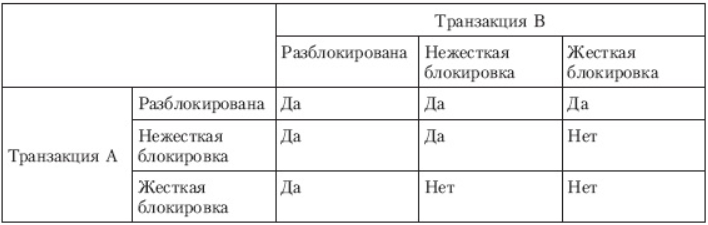
\includegraphics[width=0.8\textwidth]{assets/blocks.PNG}
    \caption{Правила применения жесткой и нежесткой блокировок транзакций}
\end{figure}


\paragraph{Двухфазный протокол синхронизационных блокировок}~\\

В базах данных и обработке транзакций двухфазная блокировка (2PL) — это метод управления параллелизмом, который гарантирует сериализуемость. Так же называют результирующий набор графиков транзакций базы данных (истории). Протокол использует блокировки, применяемые транзакцией к данным, которые могут блокировать (интерпретировать как сигналы для остановки) другие транзакции от доступа к тем же данным в течение жизни транзакции.


По протоколу 2PL блокировки (locks) применяются и удаляются в два этапа:

\begin{enumerate}
    \item Фаза расширения: блокировки берутся и ни одна блокировка не освобождается.
    \item Фаза сокращения: блокировки освобождаются и ни одна блокировка не берётся.
\end{enumerate}

В базовом протоколе используются два типа блокировок: Shared и Exclusive locks. Уточнения базового протокола могут использовать больше типов блокировок. Используя блокировки, блокирующие процессы, 2PL могут подвергаться взаимоблокировкам, которые являются результатом взаимной блокировки двух или более транзакций \autocite{Wiki}.

\paragraph{Тупиковые ситуации, их распознавание и разрушение} ~\\

Одним из наиболее чувствительных недостатков метода сериализации транзакций на основе синхронизационных захватов является возможность возникновение тупиков (deadlocks) между транзакциями.

Вот простой пример возникновения тупика между транзакциями T1 и T2:
\begin{enumerate}
    \item Транзакции T1 и T2 установили монопольные захваты объектов r1 и r2 соответственно;
    \item После этого T1 требуется совместный захват r2, а T2 - совместный захват r1;
    \item Ни одна из транзакций не может продолжаться, следовательно, монопольные захваты не будут сняты, а совместные - не будут удовлетворены.
\end{enumerate}

Поскольку тупики возможны, и никакого естественного выхода из тупиковой ситуации не существует, то эти ситуации необходимо обнаруживать и искусственно устранять.

Основой обнаружения тупиковых ситуаций является построение (или постоянное поддержание) графа ожидания транзакций. Граф ожидания транзакций - это ориентированный двудольный граф, в котором существует два типа вершин - вершины, соответствующие транзакциям, и вершины, соответствующие объектам захвата. В этом графе существует дуга, ведущая из вершины-транзакции к вершине-объекту, если для этой транзакции существует удовлетворенный захват объекта. В графе существует дуга из вершины-объекта к вершине-транзакции, если транзакция ожидает удовлетворения захвата объекта.


Легко показать, что в системе существует ситуация тупика, если в графе ожидания транзакций имеется хотя бы один цикл. Для распознавание тупика периодически производится построение графа ожидания транзакций (как уже отмечалось, иногда граф ожидания поддерживается постоянно), и в этом графе ищутся циклы. Традиционной техникой (для которой существует множество разновидностей) нахождения циклов в ориентированном графе является редукция графа.


Не вдаваясь в детали, редукция состоит в том, что прежде всего из графа ожидания удаляются все дуги, исходящие из вершин-транзакций, в которые не входят дуги из вершин-объектов. (Это как бы соответствует той ситуации, что транзакции, не ожидающие удовлетворения захватов, успешно завершились и освободили захваты). Для тех вершин-объектов, для которых не осталось входящих дуг, но существуют исходящие, ориентация исходящих дуг изменяется на противоположную (это моделирует удовлетворение захватов). После этого снова срабатывает первый шаг и так до тех пор, пока на первом шаге не прекратится удаление дуг. Если в графе остались дуги, то они обязательно образуют цикл.


Предположим, что нам удалось найти цикл в графе ожидания транзакций. Что делать теперь? Нужно каким-то образом обеспечить возможность продолжения работы хотя бы для части транзакций, попавших в тупик. Разрушение тупика начинается с выбора в цикле транзакций так называемой транзакции-жертвы, т.е. транзакции, которой решено пожертвовать, чтобы обеспечить возможность продолжения работы других транзакций. Грубо говоря, критерием выбора является стоимость транзакции; жертвой выбирается самая дешевая транзакция. Стоимость транзакции определяется на основе многофакторная оценка, в которую с разными весами входят время выполнения, число накопленных захватов, приоритет. После выбора транзакции-жертвы выполняется откат этой транзакции, который может носить полный или частичный характер. При этом, естественно, освобождаются захваты и может быть продолжено выполнение других транзакций.


Естественно, такое насильственное устранение тупиковых ситуаций является нарушением принципа изолированности пользователей, которого невозможно избежать. Заметим, что в централизованных системах стоимость построения графа ожидания сравнительно невелика, но она становится слишком большой в по-настоящему распределенных СУБД, в которых транзакции могут выполняться в разных узлах сети. Поэтому в таких системах обычно используются другие методы сериализации транзакций.


Еще одно замечание. Чтобы минимизировать число конфликтов между транзакциями, в некоторых СУБД (например, в Oracle) используется следующее развитие подхода. Монопольный захват объекта блокирует только изменяющие транзакции. После выполнении операции модификации предыдущая версия объекта остается доступной для чтения в других транзакциях. Кратковременная блокировка чтения требуется только на период фиксации изменяющей транзакции, когда обновленные объекты становятся текущими \autocite{Serial}

\subsection{Ссылочная целостность}

Ссылочная целостность. Ссылочная целостность относится непосредственно к связям между таблицами. Если кратко, то ссылочная целостность должна отвечать на вопрос: что будет со строками одной таблицы, если в связанной таблице выполняется какая-либо операция модификации? Для того чтобы понять логику ссылочной целостности, будем считать таблицу главной в паре связанных таблиц, если она содержит первичный ключ, с помощью которого осуществляется связь. Вторую таблицу будем считать подчиненной таблицей. Теперь выделим три вида операции над связанными таблицами: удаление из главной таблицы, обновление строк главной таблицы, вставка в подчиненную таблицу.

\begin{enumerate}
    \item Удаление строк из главной таблицы. Если удаляемая строка не связана со строками другой таблицы, то удалять можно без всяких последствий. Но если удаляемая строка связана со строками другой таблицы, то надо подумать, что же будет с этими строками. Просто оставить их без изменения нельзя, т. к. не понятно, как быть со значениями внешних ключей. В принципе, возможны следующие четыре сценария, поддерживаемые основными СУБД:
        \begin{itemize}
            \item строки из подчиненной таблицы должны быть удалены вместе со связанными строками из подчиненной таблицы. Такой механизм называется каскадированием;
            \item если удаляемая строка из главной таблицы связана со сроками из подчиненной таблицы, то такая операция удаления должна быть отвергнута. Данный механизм наиболее безопасен и предпочтителен при построении информационной системы;
            \item если строка в подчиненной таблице связана с удаляемой строкой в главной таблице, то внешнему ключу следует присвоить значение NULL;
            \item если строка в подчиненной таблице связана с удаляемой строкой в главной таблице, то внешнему ключу следует присвоить значение, принятое по умолчанию.
        \end{itemize}
    
    \item Обновление строк из главной таблицы. Если обновляемая строка не связана со строками другой таблицы или обновляются столбцы, не от- носящиеся к первичному ключу, то обновлять можно без всяких последствий. Но если обновляемая строка связана со строками другой таблицы и обновляется первичный ключ, то здесь, как и в предыдущем случае, возможны четыре сценария:
        \begin{itemize}
            \item первичные ключи из главной таблицы обновляются вместе с внешними ключами подчиненной таблицы. Как и в случае с подобной операцией удаления, этот механизм называется каскадированием;
            \item если обновляемая строка связана с какой-либо строкой подчиненной таблицы, то операция обновления должна быть отвергнута;
            \item если строка в подчиненной таблице связана с обновляемой строкой в главной таблице, то внешнему ключу следует присвоить значение NULL;
            \item если строка в подчиненной таблице связана с обновляемой строкой в главной таблице, то внешнему ключу следует присвоить значение, принятое по умолчанию.
        \end{itemize}

    \item Вставка строк в подчиненную таблицу. Здесь возможны следующие механизмы.
        \begin{itemize}
            \item Строка в подчиненной таблице вставляется вместе со строкой в главной таблице. Здесь важно иметь в виду, что в главной таблице для всех столбцов должны быть определены значения по умолчанию. Последовательность добавления такая: вначале добавляется строка в главную таблицу и определяется значение первичного ключа. Затем добавляется строка в подчиненную таблицу, в которой значению внешнего ключа присваивается значение первичного клю- ча в главной таблице.
            \item Строка в подчиненную таблицу добавляется только при условии, что соответствующая ей строка в главной таблице уже существует.
            \item При добавлении строки в подчиненную таблицу внешнему ключу присваивается значение NULL.
            \item При добавлении строки в подчиненную таблицу внешнему ключу присваивается значение по умолчанию.
        \end{itemize}
\end{enumerate}

В некоторых простых СУБД отсутствует возможность устанавливать связи между таблицами и, таким образом, поддерживать ссылочную целостность. В этом случае поддержание ссылочной целостности полностью ложится на плечи программиста. Другими словами, связь между таблицами должна быть реализована на уровне прикладного программного обеспечения.

\paragraph{Декларативная и процедурная ссылочные целостности} ~\\

Различают два способа реализации ограничений целостности:

\begin{itemize}
    \item Декларативная поддержка ограничений целостности.
    \item Процедурная поддержка ограничений целостности.
\end{itemize}

\begin{grayquote}
    \textbf{Декларативная поддержка ограничений целостности} заключается в определении ограничений средствами языка определения данных (DDL - Data Definition Language). Обычно средства декларативной поддержки целостности (если они имеются в СУБД) определяют ограничения на значения доменов и атрибутов, целостность сущностей (потенциальные ключи отношений) и ссылочную целостность (целостность внешних ключей). Декларативные ограничения целостности можно использовать при создании и модификации таблиц средствами языка DDL или в виде отдельных утверждений (ASSERTION).
\end{grayquote}

Например, следующий оператор создает таблицу PERSON и определяет для нее некоторые ограничения целостности:

\begin{verbatim}
CREATE TABLE PERSON
  (Pers_Id INTEGER PRIMARY KEY,
  Pers_Name CHAR(30) NOT NULL,
  Dept_Id REFERENCES DEPART(Dept_Id) ON UPDATE CASCADE ON DELETE CASCADE);
\end{verbatim}

После выполнения оператора для таблицы PERSON будут объявлены следующие ограничения целостности:

\begin{itemize}
    \item Поле Pers\_Id образует потенциальный ключ отношения.
    \item Поле Pers\_Name не может содержать null-значений.
    \item Поле Dept\_Id является внешней ссылкой на родительскую таблицу DEPART, причем, при изменении или удалении строки в родительской таблице каскадно должны быть внесены соответствующие изменения в дочернюю таблицу.
\end{itemize}

\begin{grayquote}
    \textbf{Процедурная поддержка ограничений целостности} заключается в использовании триггеров и хранимых процедур.
\end{grayquote}

Не все ограничения целостности можно реализовать декларативно. Примером такого ограничения может служить требование из примера 1, утверждающее, что поле Dept\_Kol таблицы DEPART должно содержать количество сотрудников, реально числящихся в подразделении. Для реализации этого ограничения необходимо создать триггер, запускающийся при вставке, модификации и удалении записей в таблице PERSON, который корректно изменяет значение поля Dept\_Kol. Например, при вставке в таблицу PERSON новой строки, триггер увеличивает на единицу значение поля Dept\_Kol, а при удалении строки - уменьшает. Заметим, что при модификации записей в таблице PERSON могут потребоваться даже более сложные действия. Действительно, модификация записи в таблице PERSON может заключаться в том, что мы переводим сотрудника из одного отдела в другой, меняя значение в поле Dept\_Id. При этом необходимо в старом подразделении уменьшить количество сотрудников, а в новом - увеличить \autocite{TransCit}.

\paragraph{Внешний ключ} ~\\

\begin{grayquote}
    \textbf{Внешний ключ} – это ограничение целостности, в соответствии с которым множество значений внешнего ключа является подмножеством значений первичного или уникального ключа родительской таблицы \autocite{Karpova2009}.
\end{grayquote}

Ограничение целостности по внешнему ключу проверяется в двух случаях \autocite{Karpova2009}:

\begin{itemize}
    \item при добавлении записи в подчинённую таблицу СУБД проверяет, что в родительской таблице есть запись с таким же значением первичного ключа;
    \item при удалении записи из родительской таблицы СУБД проверяет, что в подчинённой таблице нет записей с таким же значением внешнего ключа.
\end{itemize}

\paragraph{Способы поддержания ссылочной целостности} ~\\
СУБД имеют механизм автоматического поддержания ссылочной целостности. Любая операция, изменяющая данные в таблице, вызывает автоматическую проверку ссылочной целостности. При этом \autocite{WikiLink}:

\begin{itemize}
    \item При операции добавления записи автоматически проверяется, ссылаются ли внешние ключи в этой записи на существующие записи в заявленных при описании связанных таблицах. Если выясняется, что операция приведёт к появлению некорректных ссылок, она не выполняется — система возвращает ошибку.
    
    \item При операции редактирования записи проверяется:
    \begin{itemize}
        \item если изменяется её первичный ключ и на данную запись имеются ссылки, то операция редактирования завершается с ошибкой;
        \item если изменяется какой-то из внешних ключей, хранящихся в этой записи, и после изменения внешний ключ будет ссылаться на несуществующую запись, то операция редактирования завершается с ошибкой.
    \end{itemize}
    
    \item При операции удаления записи проверяется, нет ли на неё ссылок. Если ссылки имеются, то возможно три варианта дальнейших действий (фактически выполняемый зависит от СУБД и от выбора программиста, который он должен сделать при описании связи):
    \begin{itemize}
        \item Запрет — удаление блокируется и возвращается ошибка.
        \item Каскадное удаление — в одной транзакции производится удаление данной записи и всех записей, ссылающихся на данную. Если на удаляемые записи также есть ссылки и настройки также требуют удаления, то каскадное удаление продолжается дальше. Таким образом, после удаления данной записи в базе не остаётся ни одной записи, прямо или косвенно ссылающейся на неё. Если хотя бы одну из ссылающихся записей удалить не получается (либо для неё настроен запрет, либо происходит какая-либо ещё ошибка), то все удаления запрещаются.
        \item Присвоение NULL — во все внешние ключи записей, ссылающихся на данную, записывается маркер NULL. Если хотя бы для одной из ссылающихся записей это невозможно (например, если поле внешнего ключа описано как NOT NULL), то удаление запрещается.
    \end{itemize}
\end{itemize}

\subsection{Правила (триггеры)}
Триггеры являются одной из разновидностей хранимых процедур. Их исполнение происходит при выполнении для таблицы какого-либо оператора языка манипулирования данными (DML). Триггеры используются для проверки целостности данных, а также для отката транзакций.


Триггер представляет собой специальный тип хранимых процедур, запускаемых сервером автоматически при попытке изменения данных в таблицах, с которыми триггеры связаны. Каждый триггер привязывается к конкретной таблице. Все производимые им модификации данных рассматриваются как одна транзакция. В случае обнаружения ошибки или нарушения целостности данных происходит откат этой транзакции. Тем самым внесение изменений запрещается. Отменяются также все изменения, уже сделанные триггером.


Триггер представляет собой весьма полезное и в то же время опасное средство. Так, при неправильной логике его работы можно легко уничтожить целую базу данных, поэтому триггеры необходимо очень тщательно отлаживать.


В отличие от обычной подпрограммы, триггер выполняется неявно в каждом случае возникновения триггерного события, к тому же он не имеет аргументов. Приведение его в действие иногда называют запуском триггера \autocite{IntuitTrigg}

\paragraph{Цели использования правил} ~\\

С помощью триггеров достигаются следующие цели \autocite{IntuitTrigg}:
\begin{itemize}
    \item проверка корректности введенных данных и выполнение сложных ограничений целостности данных, которые трудно, если вообще возможно, поддерживать с помощью ограничений целостности, установленных для таблицы;
    \item выдача предупреждений, напоминающих о необходимости выполнения некоторых действий при обновлении таблицы, реализованном определенным образом;
    \item накопление аудиторской информации посредством фиксации сведений о внесенных изменениях и тех лицах, которые их выполнили;
    \item поддержка репликации.
\end{itemize}

\paragraph{Способы задания, моменты выполнения} ~\\

Создает триггер только владелец базы данных. Это ограничение позволяет избежать случайного изменения структуры таблиц, способов связи с ними других объектов и т.п.


Основной формат команды CREATE TRIGGER показан ниже:
\begin{verbatim}
<Определение_триггера>::=
  CREATE TRIGGER имя_триггера
  BEFORE | AFTER <триггерное_событие>
  ON <имя_таблицы>
  [REFERENCING
    <список_старых_или_новых_псевдонимов>]
  [FOR EACH { ROW | STATEMENT}]
  [WHEN(условие_триггера)]
  <тело_триггера>
\end{verbatim}

Триггерные события состоят из вставки, удаления и обновления строк в таблице. В последнем случае для триггерного события можно указать конкретные имена столбцов таблицы.

\begin{grayquote}
    \textbf{Триггер} – это процедура БД, которая привязана к конкретной таблице и вызывается автоматически при наступлении определённого события (добавления, удаления или модификации данных этой таблицы).
\end{grayquote}

В отличие от обычной подпрограммы, триггер выполняется неявно в каждом случае возникновения триггерного события, к тому же он не имеет аргументов. Приведение его в действие иногда называют запуском триггера.


Время запуска триггера определяется с помощью ключевых слов BEFORE ( триггер запускается до выполнения связанных с ним событий) или AFTER (после их выполнения).


Выполняемые триггером действия задаются для каждой строки ( FOR EACH ROW ), охваченной данным событием, или только один раз для каждого события ( FOR EACH STATEMENT ).


Обозначение <список\_старых\_или\_новых\_псевдонимов> относится к таким компонентам, как старая или новая строка ( OLD / NEW ) либо старая или новая таблица ( OLD TABLE / NEW TABLE ). Ясно, что старые значения не применимы для событий вставки, а новые – для событий удаления \autocite{IntuitTrigg}.

\subsection{События}

\paragraph{Назначение механизма событий} ~\\

Механизм событий в базе данных (database events) позволяет прикладным программам и серверу базы данных уведомлять другие программы о наступлении в базе данных определенного события и тем самым синхронизировать их работу \autocite{OSP}.

\paragraph{Сигнализаторы событий. Типы уведомлений о происхождении события. Компоненты механизма событий} ~\\

Операторы языка SQL, обеспечивающие уведомление, часто называют сигнализаторами событий в базе данных (database event alerters). Функции управления событиями целиком ложатся на сервер базы данных.


Механизм событий используется следующим образом. Вначале в базе данных для каждого события создается флажок, состояние которого будет оповещать прикладные программы о том, что некоторое событие имело место (оператор CREATE DBEVENT - СОЗДАТЬ СОБЫТИЕ). Далее во все прикладные программы, на ход выполнения которых может повлиять это событие, включается оператор REGISTER DBEVENT (ЗАРЕГИСТРИРОВАТЬ СОБЫТИЕ), который оповещает сервер базы данных, что данная программа заинтересована в получении сообщения о наступлении события. Теперь любая прикладная программа или процедура базы данных может вызвать событие оператором RAISE DBEVENT (ВЫЗВАТЬ СОБЫТИЕ). Как только событие произошло, каждая зарегистрированная программа может получить его, для чего должна запросить очередное сообщение из очереди событий (оператор GET DBEVENT - ПОЛУЧИТЬ СОБЫТИЕ) и запросить информацию о событии, в частности, его имя (оператор SQL INQUIRE\_SQL) \autocite{OSP}.

\section{Механизмы обеспечения конфиденциальности в СУБД}

4.1 Классификация угроз конфиденциальности СУБД
Причины, виды, основные методы нарушения конфиденциальности. Типы утечки конфи-денциальной информации из СУБД, частичное разглашение. Соотношение защищенности и доступности данных. Получение несанкционированного доступа к конфиденциальной инфор-мации путем логических выводов. Методы противодействия. Особенности применения криптографических методов.

4.2 Средства идентификации и аутентификации
Общие сведения. Совместное применение средств идентификации и аутентификации, встроенных в СУБД и  в ОС. 

4.3 Средства управления доступом
Основные понятия: субъекты и объекты, группы пользователей, привилегии, роли и пред-ставления. Виды привилегий: привилегии безопасности и доступа. Использование ролей и привилегий пользователей. Соотношение прав доступа, определяемых ОС и СУБД. Метки безопасности. Использование представлений для обеспечения конфиденциальности информации в СУБД.

4.4 Обеспечение конфиденциальности путем тиражирования БД 
Формальная модель для обеспечения конфиденциальности БД с помощью тиражирования. Архитектура и политика безопасности в модели SINTRA. 

4.5 Аудит и подотчетность
Подотчетность действий пользователя и аудит связанных с безопасностью событий. Реги-страция действий пользователя. Управление набором регистрируемых событий. Анализ регистрационной информации. 
\section{Механизмы, поддерживающие высокую готовность}

\underline{Определение: } Высокая доступность (High Availability, HA) - это характеристика технической системы, разработанная для избежания невыполненного обслуживания путём уменьшения или управления сбоями и минимизации времени плановых простоев \autocite{WikiHA}. Доступность часто измеряется в <<Nines>> (девятки).

Высокая готовность для каждой конкретной системы зависит от цели, для которой предназначена эта система. Для некоторых компаний высокая готовность значит максимальное downtime за год в несколько минут. Для других HA может значит downtime несколько часов в месяц.
\begin{figure}[h]
    \centering
    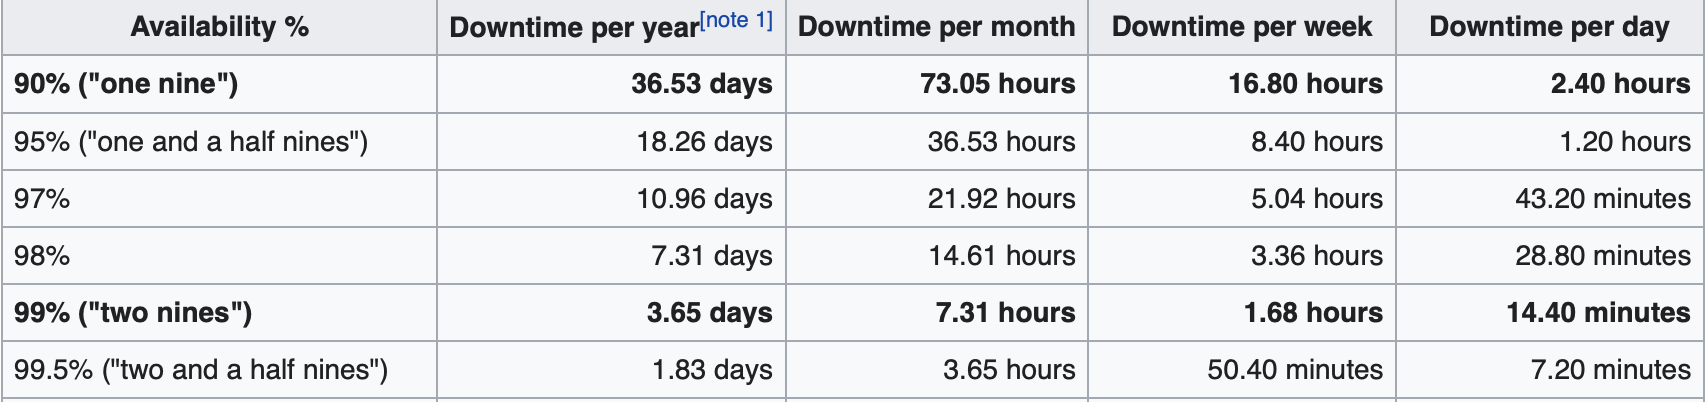
\includegraphics[width=0.8\textwidth]{assets/avail.png}
    \caption{Пример <<Nines>>}
    \label{fig:mesh1}
\end{figure}

HA включает в себя несколько важных аспектов:
\begin{enumerate}
    \item Доступность данных
    \item Защита данных
    \item Производительность
    \item Цена поддержки
\end{enumerate}

\subsection{Средства, поддерживающие высокую готовность}
\paragraph{Аппаратная и программная поддержки}
Существует несколько возможных уровней обеспечения высокой готовности системы: аппаратный и программный уровни. \\
\subsubsection{Аппаратные средства, поддерживающие высокую готовность}
\underline{Аппаратный уровень} включает в себя:
\begin{enumerate}
    \item \underline{Репликация БД}
    Репликация позволяет скопировать данные с одного сервера бд на другой.
    Существуют  два подхода репликации баз данных, рассмотрим каждый из них \autocite{Gregorchenko}:
    \begin{itemize}
        \item \underline{Репликация Master-Slave} \\В этом подходе выделяется один основной сервер базы данных, который называется Master. На нем происходят все изменения в данных (любые запросы INSERT/UPDATE/DELETE). Slave-сервер постоянно копирует все изменения с Master. С приложения на Slave-сервер могут отправляться запросы на чтение данных (запросы SELECT). Таким образом Master-сервер может отвечать за изменения данных, а Slave за чтение. Также Master сервер может отвечать за все операции с данными, а Slave являться бэкапом. При выходе из строя Slave, достаточно просто переключить все приложение на работу с Master. После этого восстановить репликацию на Slave и снова его запустить. Если выходит из строя Master, нужно переключить все операции (и чтения, и записи) на Slave. Таким образом он станет новым Master. После восстановления старого Master, настроить на нем реплику, и он станет новым Slave.
        Выше был рассмотрен случай асинхронной репликации. При синхронной репликации результат сразу же записывается и в Master, и в Slave. Возвращение управления клиенту происходит только после записи в обе базы.
        \item \underline{Репликация Master-Master}\\ В этой схеме любой из серверов может использоваться как для чтения, так и для записи. При использовании такого типа репликации достаточно выбрать случайного Master для обработки соединения, но часто один из серверов выбирается основным(Active), а другой(Passive) используется, как бэкап, в который при необходимости(в случае выхода из строя основного) можно легко начать писать данные. Репликация типа Мастер-Мастер для баз данных увеличивает скорость доступа к данным и повышает избыточность для действующих сайтов. Но данная схема обладает недостатком из-за возможных рассинхронизаций при записи данных. 
    \end{itemize}  

    Помимо разбиения репликаций по способу организации системы (см. выше) стоит выделить различные подходы по способу внесения изменений в базу данных. Рассмотрим на примере PostgreSQL, который поддерживает эти реализации \autocite{PostrgreSQL1}.
    \begin{itemize}
        \item \underline{Потоковая репликация} \\Это репликация, при которой от основного сервера PostgreSQL на реплики передается WAL(журнал предзаписи транзакций). И каждая реплика затем по этому журналу изменяет свои данные. Для настройки такой репликации все серверы должны быть одной версии, работать на одной ОС и архитектуре. Потоковая репликация в Postgres бывает двух видов — асинхронная и синхронная.
		\begin{enumerate}
        		\item{Асинхронная репликация} \\В этом случае PostgreSQL сначала применит изменения на основном узле и только потом отправит записи из WAL на реплики. Преимущество такого способа — быстрое подтверждение транзакции, т.к. не нужно ждать пока все реплики применят изменения. Недостаток в том, что при падении основного сервера часть данных на репликах может потеряться, так как изменения не успели продублироваться.
        		\item{Синхронная репликация} \\В этом случае изменения сначала записываются в WAL хотя бы одной реплики и только после этого фиксируются на основном сервере. Преимущество — более надежный способ, при котором сложнее потерять данные. Недостаток — операции выполняются медленнее, потому что прежде чем подтвердить транзакцию, нужно сначала продублировать ее на реплике.
        	\end{enumerate}
        	\item \underline{Логическая репликация} \\Логическая репликация оперирует записями в таблицах PostgreSQL. Этим она отличается от потоковой репликации, которая оперирует физическим уровнем данных: биты, байты, и адреса блоков на диске. Возможность настройки логической репликации появилась в PostgreSQL 10.
Этот вид репликации построен на механизме публикации/подписки: один сервер публикует изменения, другой подписывается на них. При этом подписываться можно не на все изменения, а выборочно. Например, на Master-сервере 50 таблиц: 25 из них могут копироваться на один Slave-сервер, а 25 — на другой.
Также есть несколько ограничений, главное из которых — нельзя реплицировать изменения структуры БД. То есть если на Master-сервере добавится новая таблица или столбец — эти изменения не попадут в Slave автоматически, их нужно применять отдельно.
В отличие от потоковой репликации, логическая может работать между разными версиями PostgreSQL, ОС и архитектурами.
	\end{itemize}
     \item \underline{RAID} - технология виртуализации данных для объединения нескольких физических дисковых устройств в логический модуль для повышения отказоустойчивости и производительности.
     Рассмотрим базовые уровни рейд массивов \autocite{Patterson}:
     \begin{enumerate}
         \item RAID 0 (striping — «чередование») — дисковый массив из двух или более жёстких дисков без резервирования. Информация разбивается на блоки данных фиксированной длины и записывается на оба/несколько дисков поочередно.
         \item RAID 1 (mirroring — «зеркалирование») — массив из двух (или более) дисков, являющихся полными копиями друг друга. Не следует путать с массивами RAID 1+0 (RAID 10), RAID 0+1 (RAID 01), в которых используются более сложные механизмы зеркалирования.
         \item RAID 2. Массивы такого типа основаны на использовании кода Хэмминга. Диски делятся на две группы: для данных и для кодов коррекции ошибок, причём если данные хранятся на $2 ^ n - n - 1$ дисках, то для хранения кодов коррекции необходимо $n$ дисков. Суммарное количество дисков при этом будет равняться $2 ^ n - 1$. Данные распределяются по дискам, предназначенным для хранения информации, так же, как и в RAID 0, то есть они разбиваются на небольшие блоки по числу дисков.
         \item В массиве RAID 3 из $n$ дисков данные разбиваются на куски размером меньше сектора (разбиваются на байты или блоки) и распределяются по $n - 1$ дискам. Ещё один диск используется для хранения блоков чётности. В RAID 2 для этой цели применялся $n - 1$ диск, но большая часть информации на контрольных дисках использовалась для коррекции ошибок «на лету», в то же время большинство пользователей устраивает простое восстановление информации в случае её повреждения, для чего хватает данных, умещающихся на одном выделенном жёстком диске. \\ Отличия RAID 3 от RAID 2: невозможность коррекции ошибок на лету.
         \item RAID 4 похож на RAID 3, но отличается от него тем, что данные разбиваются на блоки, а не на байты. Таким образом, удалось отчасти «победить» проблему низкой скорости передачи данных небольшого объёма. Запись же производится медленно из-за того, что чётность для блока генерируется при записи и записывается на единственный диск.
         \item RAID 5. Основным недостатком уровней RAID от 2-го до 4-го является невозможность производить параллельные операции записи, так как для хранения информации о чётности используется отдельный контрольный диск. RAID 5 не имеет этого недостатка. Блоки данных и контрольные суммы циклически записываются на все диски массива, нет асимметричности конфигурации дисков. Под контрольными суммами подразумевается результат операции XOR (исключающее или). XOR обладает особенностью, которая даёт возможность заменить любой операнд результатом, и, применив алгоритм XOR, получить в результате недостающий операнд.
         \item RAID 6 — похож на RAID 5, но имеет более высокую степень надёжности — два (или более) диска данных и два диска контроля чётности. Основан на кодах Рида — Соломона и обеспечивает работоспособность после одновременного выхода из строя любых двух дисков. Обычно использование RAID 6 вызывает примерно 10-15 \% падение производительности дисковой группы, относительно RAID 5, что вызвано б\'{о}льшим объёмом работы для контроллера (более сложный алгоритм расчёта контрольных сумм), а также необходимостью читать и перезаписывать больше дисковых блоков при записи каждого блока.
     \end{enumerate}
     Также существуют различные комбинации данных подходов.
\end{enumerate}
\subsubsection{Программные средства, поддерживающие высокую готовность}
\underline{Программные подходы}:
\begin{enumerate}
    \item \underline{Автоматический перезапуск экземпляров БД, сетевых демонов и других ресурсов}
    \item \underline{Защита от повреждения данных(Data corruption protection)}
    \begin{itemize}
        \item Использование контрольных чек-сумм
        \item Автоматическое восстановление из резервной копии или повторная передача
    \end{itemize}
    \item \underline{PITR (Point In Time Recovery)} это технология, используемая в базах данных для восстановления данных на конкретный момент времени. Эта функция необходима для восстановления после случайного удаления данных, их повреждения или других непредвиденных проблем. Вот краткое описание работы PITR и её преимуществ:
    \begin{itemize}
        \item Непрерывное резервное копирование: \\
        PITR включает непрерывное резервное копирование журналов транзакций базы данных, помимо регулярных полных резервных копий. Эти журналы транзакций фиксируют каждое изменение, сделанное в базе данных, что позволяет точно восстановить данные.
        \item Процесс восстановления: \\
        Для выполнения PITR необходимо начать с последней полной резервной копии, а затем применить журналы транзакций до желаемого момента времени. Этот момент может быть любым до возникновения повреждения или потери данных.
        \item Гибкость и точность: \\
        Этот метод позволяет очень точно восстановить данные, вплоть до конкретной минуты или даже секунды, в зависимости от частоты логирования. Это особенно полезно для минимизации потерь данных во время восстановления.
        \item Сценарии использования: \\
        PITR идеально подходит для восстановления после ошибок пользователя, таких как случайное удаление или изменение данных, а также после определённых видов повреждения данных. Эта технология позволяет отменить нежелательные изменения без значительных потерь данных.
        \item Реализация: \\
        Различные системы баз данных реализуют PITR по-разному. Например, PostgreSQL использует Write-Ahead Logging (WAL) для PITR, где файлы WAL содержат необходимую информацию для восстановления состояния базы данных. Oracle, MySQL и SQL Server имеют свои собственные методы обработки журналов транзакций и выполнения PITR.
    \end{itemize}
    \item \underline{Application continuity (Oracle)} \cite{availability-ApplicationContinuity} это технология, разработанная для повышения надежности и устойчивости работы приложений при сбоях. Она позволяет приложениям автоматически восстанавливать выполнение транзакций, минимизируя влияние на конечных пользователей. Вот основные аспекты этой технологии:
    \begin{itemize}
        \item Непрерывность транзакций: \\
        Application Continuity обеспечивает автоматическое повторное выполнение транзакций после сбоев. Это означает, что при сбое соединения с базой данных или при перезагрузке сервера транзакции продолжаются с того места, где они были прерваны, без необходимости вмешательства пользователя.
        \item Механизм работы: \\
        Технология сохраняет состояние транзакции и контекст выполнения, а затем использует эти данные для восстановления и повторного выполнения операций. Это включает в себя сохранение всех вызовов SQL и PL/SQL, которые приложение выполняло до сбоя.
        \item Прозрачность для пользователей: \\
        Пользователи не замечают сбоев, так как восстановление происходит прозрачно для них. Это обеспечивает высокую степень удовлетворенности пользователей и повышает доверие к системе.
        \item Интеграция и использование: \\
        Application Continuity интегрируется с Oracle Database и поддерживается в различных архитектурах, включая Oracle Real Application Clusters (RAC) и Oracle Active Data Guard. Это позволяет использовать технологию в масштабируемых и распределенных системах.
        \item Преимущества: \\
        Основные преимущества включают снижение риска потери данных, повышение доступности приложений и улучшение пользовательского опыта. Технология помогает обеспечить высокие уровни SLA (Service Level Agreement) за счет минимизации простоев.
    \end{itemize}
    \item \underline{WAL} Данный подход будет описан ниже.
\end{enumerate}

\subsubsection{Кластерная организация серверов баз данных}

Кластеризация базы данных - это процесс объединения нескольких серверов или инстансов, соединяющих одну базу данных. Иногда одного сервера может быть недостаточно для управления объемом данных или количеством запросов, тогда возникает необходимость в кластере. 
 
К общим требованиям, предъявляемым к кластерным системам, относятся:
\begin{enumerate}
    \item Высокая готовность
    \item Высокое быстродействие
    \item Масштабирование
    \item Удобство обслуживания
\end{enumerate}

Кластеры баз данных являются распространенной технологией.  Рассмотрим три типа архитектуры кластерных вычислений. Отказоустойчивые кластеры, высокопроизводительные кластеры и кластеры балансировки нагрузки.

\begin{enumerate}
\item Отказоустойчивые / высокодоступные кластеры. Кластер обеспечивает доступность сервиса путем репликации серверов и избыточной реконфигурации программного и аппаратного обеспечения. Таким образом, каждая система контролирует другую и работает на запросы, если какой-либо один из узлов выходит из строя.

\item Высокопроизводительные кластеры. Целью разработки высокопроизводительных кластеров баз данных является создание высокопроизводительных компьютерных систем. Основная цель - разумное распределение рабочей нагрузки.

\item Кластеры балансировки нагрузки. Эти кластеры базы данных служат для распределения нагрузки между различными серверами. Они стремятся обеспечить увеличенную пропускную способность сети, в конечном итоге увеличивая производительность. Системы в этой сети объединяют свои узлы, с помощью которых пользовательские запросы равномерно распределяются между участвующими узлами.
\end{enumerate}

Несмотря на всю распределенную систему на заднем плане, пользователю это кажется единой системой. Использование кластеров варьируется от предприятия к предприятию, в зависимости от вида процессов и требуемого уровня производительности.
\subsubsection{Параметры настройки СУБД}
Для обеспечения высокой доступности (HA) в системах управления базами данных (СУБД) необходимо правильно настроить различные параметры. Вот основные параметры настройки, относящиеся к HA, на примере таких СУБД как PostgreSQL, Oracle и MySQL:
\paragraph{PostgreSQL} \cite{availability-postgres}
\begin{enumerate}
    \item Streaming Replication:
    \begin{itemize}
        \item wal\_level: Установите значение replica для включения репликации.
        \item max\_wal\_senders: Указывает максимальное количество процессов отправки WAL (Write-Ahead Logging).
        \item wal\_keep\_segments: Определяет, сколько сегментов WAL следует сохранять для репликации.
        \item archive\_mode и archive\_command: Включите архивирование WAL для обеспечения PITR (Point-In-Time Recovery).
    \end{itemize}
    \item Hot Standby:
    \begin{itemize}
        \item hot\_standby: Установите on, чтобы разрешить выполнение запросов на репликах.
        \item max\_standby\_streaming\_delay: Задает максимальную задержку для потоковой реплики перед откатом длительных транзакций.
    \end{itemize}
    \item Failover: Используйте инструменты, такие как Patroni, pg\_auto\_failover или repmgr, для автоматического переключения на резервный сервер при сбое основного.
\end{enumerate}
\paragraph{Oracle} \cite{availability-oracle}
\begin{enumerate}
    \item Oracle Real Application Clusters (RAC):
    \begin{itemize}
        \item Cluster Interconnect: Настройте высокоскоростную сеть для обмена данными между узлами кластера.
        \item Instance Caging: Ограничьте ресурсы CPU для каждого экземпляра в кластере.
    \end{itemize}
    \item Data Guard:
    \begin{itemize}
        \item Redo Transport Services: Настройте передачу журналов redo на резервные серверы.
        \item Standby Redo Logs: Настройте резервные журналы redo для повышения производительности репликации.
        \item Data Guard Broker: Используйте для управления и автоматизации процессов Data Guard.
    \end{itemize}
    \item Flashback Technology:
    \begin{itemize}
        \item db\_flashback\_retention\_target: Установите цель времени для хранения данных Flashback.
        \item undo\_retention: Настройте для обеспечения длительных операций отката.
    \end{itemize}
\end{enumerate}
\paragraph{MySQL} \cite{availability-mysql}
\begin{enumerate}
    \item Replication:
    \begin{itemize}
        \item server\_id: Уникальный идентификатор сервера для репликации.
        \item log\_bin: Включите бинарные логи для записи всех изменений.
        \item binlog\_format: Установите формат бинарного лога (например, ROW для строковой репликации).
        \item relay\_log: Определите журналы ретрансляции для реплики.
    \end{itemize}
    \item Group Replication:
    \begin{itemize}
        \item group\_replication\_group\_name: Уникальное имя группы репликации.
        \item group\_replication\_start\_on\_boot: Автоматически запускать репликацию при запуске сервера.
        \item group\_replication\_bootstrap\_group: Используйте для инициализации группы.
    \end{itemize}
    \item High Availability Tools:
    \begin{itemize}
        \item Используйте MySQL InnoDB Cluster, ProxySQL и MHA (Master High Availability Manager) для автоматизации failover и балансировки нагрузки.
    \end{itemize}
\end{enumerate}
\subsubsection{Сохранение и восстановление БД}

Основным свойством транзакций СУБД является durability. Идея механизма обеспечения этого свойства является одинаковой для всех СУДБ \autocite{PostrgreSQL1}. СУБД использует специальны
Следовательно, с точки зрения файловой системы INSERT и UPDATE не являются атомарными операциями: если кто-то внезапно выключит ваш сервер, данные окажутся испорчены. Если возникает сбой, база данных использует этот файл для того, чтобы восстановить данные на момент падения. WAL -- это бинарный лог, так что для его чтения нужна специальная утилита.
Например в PostreSQL данный файл называется WAL и лежит по пути \$PGDATA/pg\_xlog.
PostgreSQL позволяет отключать WAL для отдельных таблиц, помечая их как UNLOGGED.

\subsection{Оперативное администрирование}
\subsubsection{Задачи, средства и режимы администрирования}

Задачи администратора баз данных могут незначительно отличаться в зависимости от вида применяемой СУБД, но в основные задачи входит:
\begin{itemize}
    \item Проектирование базы данных.
    \item Оптимизация производительности базы данных.
    \item Резервирование и восстановление базы данных.
    \item Обеспечение целостности баз данных.
    \item Обеспечение перехода на новую версию СУБД.
\end{itemize}
Существуют различные программы и способы администрирования БД, которые напрямую зависят от БД. Основным инструментом работы с базой данных является DSL и программы, например для Oracle можно использовать SQL Developer. Существуют программы, поддерживающие работу с любой БД, например продукты JetBrains.  Также отдельно существуют средства мониторинга серверов.
\subsubsection{Мониторинг серверов СУБД}
Мониторинг СУБД можно условно разделить на два типа:
\begin{enumerate}
    \item Мониторинг средствами СУБД
    \item Мониторинг хостов и сервисов, на которых запущена БД.
\end{enumerate}
\underline{Мониторинг средствами СУБД} \\ Средства мониторинга, предоставляемые СУБД зависят в первую очередь от конкретной реализации этой системы, однако можно выделить метрики, которые в большинстве случаев собираются встроенным мониторингом. В первую очередь это объем операций ввода/вывода, необходимых для исполнения транзакции, утилизация процессоров и временем отклика системы. Наиболее распространенной метрикой оценки производительности системы является ее время отклика, которое представляет собой интервал времени, в течении которого сервер возвращает первую строку результата исполнения запроса, т.е. пользователь получает визуальное подтверждение того, что его запрос исполняется. Пропускная способность обслуживаемых сервером процессов и пользователей определяет сколько запросов возможно исполнить в фиксированный интервал времени, и сколько строк и какого размера возвращается клиенту. При увеличении числа активных процессов и/или пользователей, возрастает и их конкуренция за системные ресурсы. Результатом такой чрезмерной нагрузки может стать увеличение времени отклика и снижение общей пропускной способности. Большое влияние на производительности базы данных оказывает также физическая и логическая целостность данных. \\
\underline{Мониторинг хостов и сервисов, на которых запущена БД} \\ Рассмотрим две системы - немного устаревший, но еще использующийся Zabbix и более современный и активно набирающий популярность Prometheus \autocite{Prometheus-vs-Zabbix}.
\begin{itemize}

	\item \underline{Zabbix}\\ Многофункциональным средством является Zabbix — свободная система мониторинга и отслеживания статусов разнообразных сервисов компьютерной сети, серверов и сетевого оборудования. Он поддерживает несколько видов мониторинга. Simple checks — может проверять доступность и реакцию стандартных сервисов, таких как SMTP или HTTP без установки какого-либо программного обеспечения на наблюдаемом хосте. Zabbix agent — может быть установлен на UNIX-подобных или Windows хостах для получения данных о нагрузке процессора, использования сети, дисковом пространстве и так далее. External check — выполнение внешних программ. 
	С точки зрения пользователя Zabbix разделен на две большие части: сервер и агенты. Сервер расположен на одной машине, которая собирает и хранит статистические данные, а агенты располагаются на тех машинах, с которых собираются данные. Агенты Zabbix поддерживают как пассивные (polling), так и активные проверки (trapping). Пассивные проверки означают, что сервер Zabbix запрашивает значение у агента Zabbix, а агент обрабатывает запрос и возвращает значение серверу Zabbix. Активные проверки означают, что агент Zabbix запрашивает список активных проверок с сервера Zabbix, а затем периодически отправляет результаты.
	Важной особенностью Zabbix является способ хранения данных. Для своей работы данное средство при установке требует подключения внешней базы данных (MySQL, PostgreSQL, Oracle и т.д.).
	Также стоит отметить, что Zabbix не так гибок в запросах. Он использует ключи элементов для получения метрик.
	\item \underline{Prometheus}\\ Prometheus — это система мониторинга с открытым исходным кодом, предоставляющая своим пользователям мощный язык запросов, функции хранения и визуализации. Он собирает метрики в реальном времени и записывает их в базу данных временных рядов. Prometheus предоставляет многомерную модель данных, которая позволяет определять метрики по именам и/или тегам, чтобы идентифицировать их как часть уникального временного ряда. Благодаря большому сообществу многие сервисы могут отправлять метрики в формате Prometheus. Если какие-то сервисы не могут этого сделать, то есть множество библиотек, помогающих в экспорте существующих метрик из сторонних систем в виде метрик Prometheus. 
	Prometheus для хранения данных использует свою базу данных временных рядов (TSDB). Используя собственную TSDB, Prometheus может получать и обрабатывать несравненно больше метрик, чем многие другие системы мониторинга. Данные могут быть записаны даже с отметками времени с миллисекундным разрешением. 
	В отличие от Zabbix Prometheus является более гибким в плане выполнения запросов. Prometheus предоставляет собственный функциональный язык для запросов, который называется PromQL (Prometheus Query Language). PromQL невероятно гибкий, простой и мощный. Он может применять функции и операторы к вашим запросам метрик, фильтровать, группировать по меткам и использовать регулярные выражения для улучшения сопоставления и фильтрации.
\end{itemize} 

\subsection{Функциональная насыщенность СУБД}
\paragraph{Формы избыточности}
Системы, обеспечивающие непрерывный доступ к данным (fault tolerant) или почти
непрерывный (high availability) обычно опираются на различные формы избыточности.
Как правило, это системы дублирования аппаратного обеспечения и контролируемой
избыточности данных \autocite{Baron}.

\paragraph{Избыточность данных}
Нормальная форма — свойство отношения в реляционной модели данных, характеризующее его с точки зрения избыточности, потенциально приводящей к логически ошибочным результатам выборки или изменения данных. Нормальная форма определяется как совокупность требований, которым должно удовлетворять отношение.

Процесс преобразования отношений базы данных к виду, отвечающему нормальным формам, называется нормализацией. Нормализация предназначена для приведения структуры БД к виду, обеспечивающему минимальную логическую избыточность, и не имеет целью уменьшение или увеличение производительности работы или же уменьшение или увеличение физического объёма базы данных. Конечной целью нормализации является уменьшение потенциальной противоречивости хранимой в базе данных информации. Как отмечает К. Дейт,общее назначение процесса нормализации заключается в следующем:
\begin{itemize}
    \item исключение некоторых типов избыточности;
    \item устранение некоторых аномалий обновления;
    \item разработка проекта базы данных, который является достаточно «качественным» представлением реального мира, интуитивно понятен и может служить хорошей основой для последующего расширения;
    \item упрощение процедуры применения необходимых ограничений целостности.
\end{itemize}

Устранение избыточности производится, как правило, за счёт декомпозиции отношений таким образом, чтобы в каждом отношении хранились только первичные факты (то есть факты, не выводимые из других хранимых фактов). \\

\paragraph{Аппаратная избыточность}
Аппаратная избыточность может включать платформы с полным резервированием, поддерживающие (standby) процессоры, диски с двойным интерфейсом (dual-port), дисковые массивы и пр. Один из вариантов - зеркалирование дисков, когда один диск используется в качестве копии другого и может быть использован при сбое вместо него. Хотя аппаратная избыточность и важна для повышения общей надежности системы, ее реализация, как правило, не ориентирована на обработку транзакций СУБД и на связанные с этим специфические ограничения, например, обеспечение атомарности транзакции. В результате СУБД не может воспользоваться преимуществами чисто аппаратных решений резервирования cистемы для повышения своей производительности.
\paragraph{Программное зеркалирование} 

Программное зеркалирование дисков, называемое также дуплексированием (duрlexing) или мультиплексированием (multiplexing), может не только защитить от аппаратных сбоев, но и улучшить производительность. Поскольку зеркалирование базы данных (или ее частей - таблиц(ы), индексов, их фрагментов и пр.) производится на другом физическом устройстве, то операции чтения данных можно распределить между двумя устройствами и производить параллельно. Конечно, зеркалирование бесполезно с любой точки зрения, если оно организовано на одном диске \autocite{Baron}.
В случае повреждения зеркалируемого диска все операции автоматически переносятся на исправный диск, сбойный диск выводится в отключенное состояние, причем приложения не замечают каких-либо изменений в конфигурации системы.
После замены неисправного диска параллельно с работой пользователей запускается процесс оперативной синхронизации зеркальных дисков (on-line remirroring), на физическом уровне копирующий рабочий диск. \\
\paragraph{Тиражирование данных}
Тиражирование в системах, требующих в первую очередь повышенной надежности, в
целом подобно зеркалированию, но здесь копия данных может поддерживаться
удаленно. Если происходит копирование всей базы данных, то обычно это делается с
целью обеспечить горячий резерв (warm standby). Однако в некоторых реализациях
есть возможность использовать копию для просмотра (без модификации) данных \autocite{Baron}. Это способно обеспечить значительные преимущества для систем со смешанной загрузкой, поскольку приложения для принятия решений, генерации отчетов и т.п,
могут обращаться к копии базы данных, в то время как приложения оперативной обработки транзакций используют первичную базу данных.
\subsection{Системы, обладающие свойством высокой готовности}
\paragraph{Casandra}~\\
Casandra - распределённая система управления базами данных, относящаяся к классу NoSQL-систем и рассчитанная на создание высокомасштабируемых и надёжных хранилищ огромных массивов данных, представленных в виде хэша \autocite{casandra}. \\
Хранилище само позаботится о проблемах наличия единой точки отказа (single point of failure), отказа серверов и о распределении данных между узлами кластера (cluster node). При чем, как в случае размещения серверов в одном центре обработки данных (data center), так и в конфигурации со многими центрами обработки данных, разделенных расстояниями и, соответственно, сетевыми задержками. Под надёжностью понимается итоговая согласованность (eventual consistency) данных с возможностью установки уровня согласования данных (tune consistency) каждого запроса. \\
Узлы кластера Casandra равноценны, и клиенты могут соединятся с любым из них, как для записи, так и для чтения. Запросы проходят стадию координации, во время которой, выяснив при помощи ключа и разметчика на каких узлах должны располагаться данные, сервер посылает запросы к этим узлам. Будем называть узел, который выполняет координацию — координатором (coordinator), а узлы, которые выбраны для сохранения записи с данным ключом — узлами-реплик (replica nodes). Физически координатором может быть один из узлов-реплик — это зависит только от ключа, разметчика и меток.
Для каждого запроса, как на чтение, так и на запись, есть возможность задать уровень согласованности данных. \\
Когда данные приходят после координации на узел непосредственно для записи, то они попадают в две структуры данных: в таблицу в памяти (memtable) и в журнал закрепления (commit log). Таблица в памяти существует для каждого колоночного семейства и позволяет запомнить значение моментально. Технически это хеш-таблица (hashmap) с возможностью одновременного доступа (concurrent access) на основе структуры данных, называемой “списками с пропусками” (skip list). Журнал закрепления один на всё пространство ключей и сохраняется на диске. Журнал представляет собой последовательность операций модификации. Так же он разбивается на части при достижении определённого размера.
Такая организация позволяет сделать скорость записи ограниченной скоростью последовательной записи на жесткий диск и при этом гарантировать долговечность данных (data durability). Журнал закрепления в случае аварийного останова узла читается при старте сервиса Casandra и восстанавливает все таблицы в памяти. Получается, что скорость упирается во время последовательной записи на диск, а у современных жёстких дисков это порядка 100МБ/с. По этой причине журнал закрепления советуют вынести на отдельный дисковый носитель.

\begin{figure}[h]
    \centering
    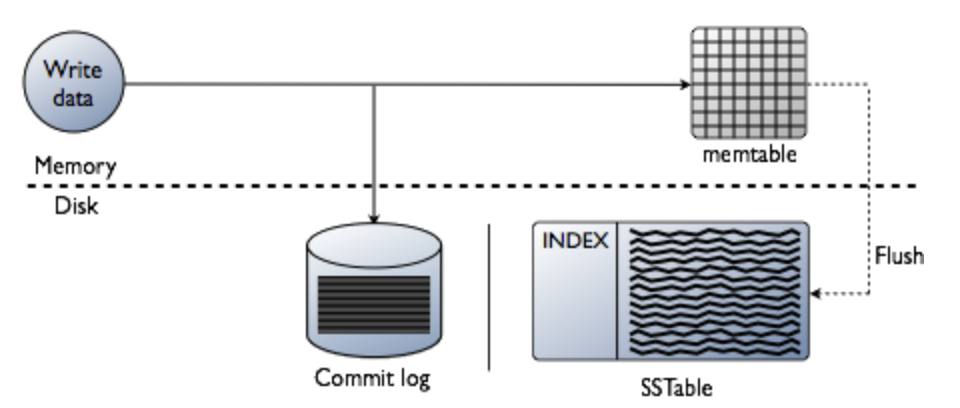
\includegraphics[width=0.8\textwidth]{assets/casandra.png}
    \caption{Схема записи в Casandra}
    \label{fig:mesh2}
\end{figure}

\paragraph{PostreSQL + Patroni}

Patroni — это Python-приложение для создания высокодоступных PostgreSQL кластеров на основе потоковой репликации. С его помощью можно преобразовать систему из ведущего и ведомых узлов (primary — replica) в высокодоступный кластер с поддержкой автоматического контролируемого (switchover) и аварийного (failover) переключения. Patroni позволяет легко добавлять новые реплики в существующий кластер, поддерживает динамическое изменение конфигурации PostgreSQL одновременно на всех узлах кластера и множество других возможностей, таких как синхронная репликация, настраиваемые действия при переключении узлов, REST API, возможность запуска пользовательских команд для создания реплики вместо pg basebackup, взаимодействие с Kubernetes и т.д. \autocite{Klyukin} \\

Опишем, как используется Patroni. Сама по себе потоковая репликация не является достаточным средством обеспечения высокой доступности. Потому что нет никакого встроенного решения, которое бы позволило перевести standby в режим нового мастера, если что-то произошло со старым мастером. Рассмотрим на примере \autocite{Aristov}.\\
Возьмем кластер из двух нод, и, допустим, у нас есть программа, запущенная на standby-сервере, мониторящая, жив ли основной сервер, и при его падении повышающая реплику до основного сервера:

\begin{figure}[h]
    \centering
    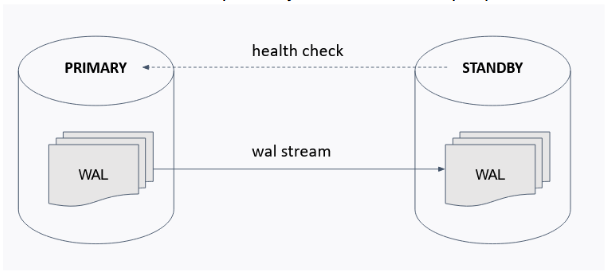
\includegraphics[width=0.8\textwidth]{assets/Patroni1.png}
    \caption{Кластер из двух нод}
    \label{fig:mesh3}
\end{figure}

Вроде всё хорошо, но что произойдёт, если у нас просто случится обрыв сетевого подключения между серверами?

\begin{figure}[h]
    \centering
    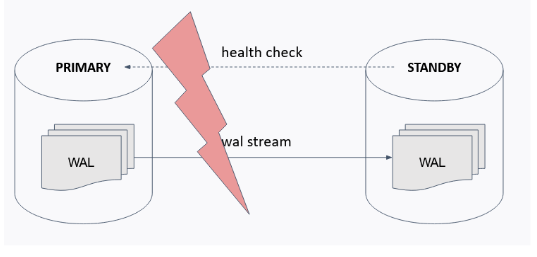
\includegraphics[width=0.8\textwidth]{assets/Patroni2.png}
    \caption{Кластер из двух нод}
    \label{fig:mesh4}
\end{figure}

Правильно! Получим два независимых основных кластера, каждый из них будет принимать запросы на запись, и мы получим такую ситуацию:

\begin{figure}[h]
    \centering
    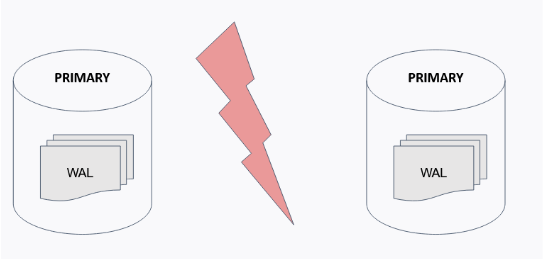
\includegraphics[width=0.8\textwidth]{assets/Patroni3.png}
    \caption{Разрыв соединения в кластере из двух нод}
    \label{fig:mesh5}
\end{figure}

Она называется splitbrain. Это очень плохая ситуация, и в дальнейшем объединить изменённые данные с двух независимых серверов без потерь практически нереально.
Казалось бы, есть простое решение - добавить стороннего наблюдателя.
Что же может пойти не так в данной конфигурации:

\begin{figure}[h]
    \centering
    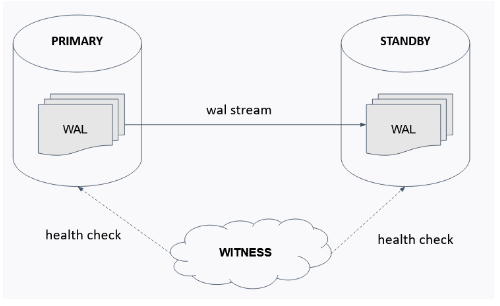
\includegraphics[width=0.8\textwidth]{assets/Patroni4.png}
    \caption{Кластер из двух нод со сторонним наблюдателем}
    \label{fig:mesh6}
\end{figure}

В такой конфигурации могут возникнуть две проблемы: во-первых, может умереть наблюдатель и мониторить станет некому, во-вторых, может оборваться соединение с основной нодой и опять мы получаем splitbrain. 

И Patroni предлагает решение данной проблемы - это использование отказоустойчивого кластера для наблюдателя, в котором мы будем хранить статус активного сервера. То есть основной будет активно ходить и поддерживать статус основного, а остальные будут опрашивать жив ли основной сервер. При потере с ним соединения через некоторое время произойдут выборы и вторичный сервер станет основным и будет активно поддерживать свой статус в этом отказоустойчивом наблюдателе. При этом изначальный основной сервер при недоступности кластера наблюдения перейдёт в статус “только чтение".

\begin{figure}[h]
    \centering
    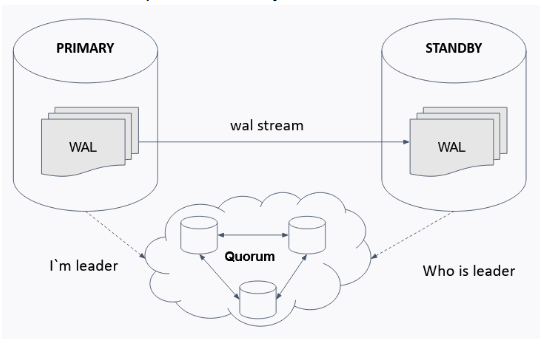
\includegraphics[width=0.8\textwidth]{assets/Patroni5.png}
    \caption{Решение, используемое в Patroni}
    \label{fig:mesh7}
\end{figure}

Quorum позволяет нам решать сложные задачи разрешения партицирования сети. Когда какой-то сегмент сети недоступен, то несколько других сегментов могут принимать решения. А изолированный сегмент в этом случае должен остановить старого мастера. 


\section{Защита данных в распределенных системах}
\subsection{Распределенные вычислительные среды}
Распределённая обработка данных - методика выполнения прикладных программ группой систем.
При этом пользователь получает возможность работать с сетевыми службами и прикладными процессами,
расположенными в нескольких взаимосвязанных абонентских системах. \autocite{Sergeeva}

\paragraph{
    Распределенная обработка информации в среде клиент-сервер.
    Концепция распределенной вычислительной среды Distributed Computing Environment (DCE).
    Распределенные базы данных в сетях ЭВМ
} ~\\

Компьютер (или программу), управляющий ресурсом, называют сервером этого ресурса (файлсервер, сервер базы данных,
вычислительный сервер...). Клиент и сервер какого-либо ресурса могут находиться как в рамках одной вычислительной системы,
так и на различных компьютерах, связанных сетью. Основной принцип технологии "клиент-сервер" заключается в разделении
функций приложения на три группы \autocite{4studClntSrv}:
\begin{itemize}
    \item ввод и отображение данных (взаимодействие с пользователем);
    \item прикладные функции, характерные для данной предметной области;
    \item функции управления ресурсами (файловой системой, базой данных и т.д.)
\end{itemize}

Поэтому, в любом приложении можно выделить следующие компоненты:
\begin{itemize}
    \item компонент представления данных
    \item прикладной компонент
    \item компонент управления ресурсом
\end{itemize}

Связь между компонентами осуществляется по определенным правилам, которые называют "протокол взаимодействия".
Каждый из компонентов приложения при этом может работать на выделенном сервере (узле) или разделять ресурсы сервера
с другими компонентами приложения. В связи с этим можно выделить следующие модели приложений:
\begin{itemize}
    \item двухзвенная модель (модель «клиент-сервер»)
    \item трехзвенная модель (модель сервера приложений)
    \item многозвенная модель
\end{itemize}

\textbf{Двухзвенная модель} позволяет распределить различным образом три компонента приложения между двумя узлами 
\textbf{Трехзвенная модель} предполагает выделение для каждого из трех компонентов приложения свой сервер \autocite{4studClntSrv}.
\textbf{Многозвенная модель} позволяет отдельным компонентам использовать ресурсы нескольких серверов, например,
распределенные базы данных. Компанией Gartner Group, специализирующейся в области исследования информационных технологий,
предложена следующая классификация двухзвенных моделей взаимодействия клиент-сервер \autocite(bmstu)

\begin{figure}[h!]
    \centering
    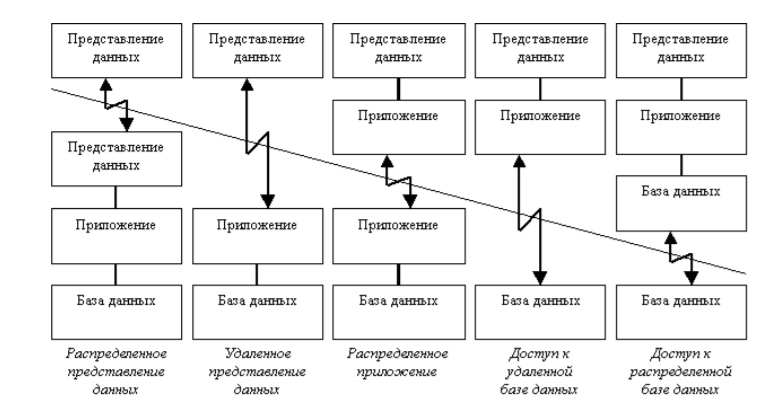
\includegraphics[width=0.8\textwidth]{assets/dce.jpg}
    \caption{Классификация двухзвенных моделей}
\end{figure}

\subsubsection{Двухзвенная структура}~\\
В любой сети, построенной на современных сетевых технологиях, присутствуют элементы
клиент-серверного взаимодействия,часто на основе двухзвенной архитектуры.

\begin{figure}[h!]
    \centering
    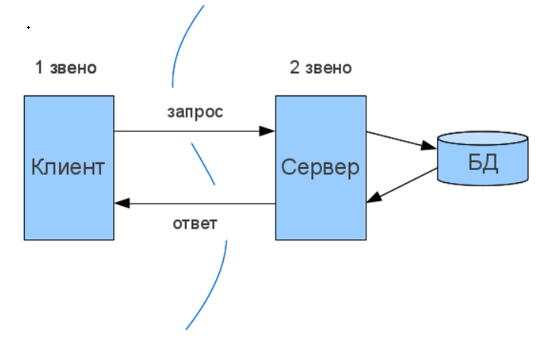
\includegraphics[width=0.8\textwidth]{assets/662}
    \caption{Двухзвенная архитектура}
\end{figure}

Двухзвенная архитектура используется в клиент-серверных системах, где сервер отвечает
на клиентские запросы напрямую и в полном объеме, при этом используя только
собственные ресурсы. Т.е. сервер не вызывает сторонние сетевые приложения и не
обращается к сторонним ресурсам для выполнения какой-либо части запроса.

\begin{figure}[h!]
    \centering
    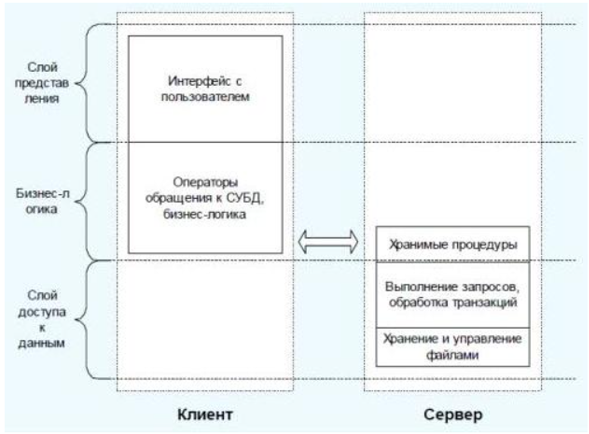
\includegraphics[width=0.8\textwidth]{assets/663}
    \caption{Типичный пример двухзвенной модели}
\end{figure}~\\

Клиентская программа работает с данными через запросы к серверному ПО. Базовые
функции приложения разделены между клиентом и сервером.

Плюсы:
\begin{itemize}
    \item Отсутствие дублирования кода программы-сервера программами-клиентами.
    \item Так как все вычисления выполняются на сервере, то требования к компьютерам, на которых установлен клиент, снижаются.
    \item Все данные хранятся на сервере, который, как правило, защищён гораздо лучше большинства клиентов. На сервере проще обеспечить контроль полномочий, чтобы разрешать доступ к данным только клиентам с соответствующими правами доступа.
    \item Позволяет объединить различные клиенты. Использовать ресурсы одного сервера часто могут клиенты с разными аппаратными платформами, операционными системами и т. п.
    \item Позволяет разгрузить сети за счёт того, что между сервером и клиентом передаются небольшие порции данных.
\end{itemize}

Минусы:
\begin{itemize}
    \item 	Бизнес логика приложений осталась в клиентском ПО. При любом изменении алгоритмов, надо обновлять пользовательское ПО на каждом клиенте.
    \item Высокие требования к пропускной способности коммуникационных каналов с сервером, что препятствует использование клиентских станций иначе как в локальной сети.
    \item Слабая защита данных от взлома, в особенности от недобросовестных пользователей системы.
    \item Высокая сложность администрирования и настройки рабочих мест пользователей системы.
    \item Необходимость использовать мощные ПК на клиентских местах.
    \item Высокая сложность разработки системы из-за необходимости выполнять бизнес-логику и обеспечивать пользовательский интерфейс в одной программе.
\end{itemize}

\subsubsection{Трехзвенная архитектура}~\\

Еще одна тенденция в клиент-серверных технологиях связана со все большим
использованием распределенных вычислений. Они реализуются на основе модели сервера
приложений, где сетевое приложение разделено на две и более частей, каждая из которых
может выполняться на отдельном компьютере. Выделенные части приложения
взаимодействуют друг с другом, обмениваясь сообщениями в заранее согласованном
формате. В этом случае двухзвенная клиент-серверная архитектура становится
трехзвенной.  На этой архитектуре построены большинство современных web-приложений.~\\

\begin{figure}[h!]
    \centering
    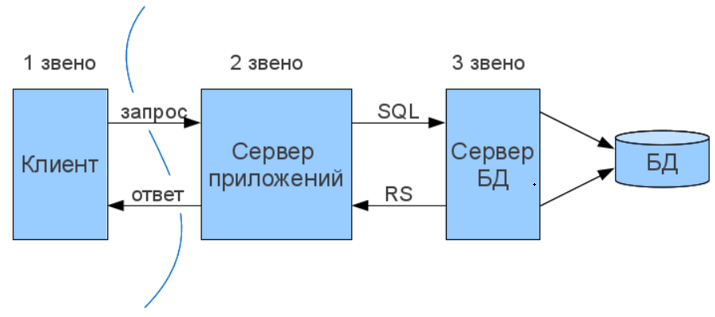
\includegraphics[width=0.8\textwidth]{assets/664}
    \caption{Трехзвенная архитектура}
\end{figure}

Основным ее отличием от предыдущей архитектуры является физическое разделение
программ, отвечающих за хранение данных (СУБД) от программ эти данные
обрабатывающих. Такое разделение программных компонент позволяет оптимизировать
нагрузки как на сетевое, так и на вычислительное оборудование комплекса.~\\

\begin{figure}[h!]
    \centering
    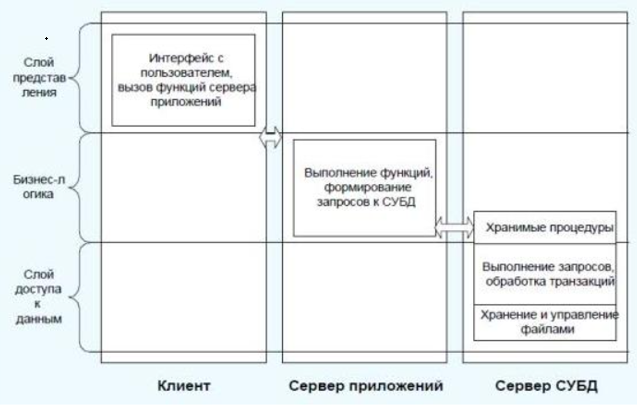
\includegraphics[width=0.8\textwidth]{assets/665}
    \caption{Типичный пример трехзвенной модели}
\end{figure}

Компоненты трехзвенной архитектуры, с точки зрения программного обеспечения
реализуют определенные сервера БД, web-сервера и браузеры. Место любого из этих
компонентов может занять программное обеспечение любого производителя.~\\

Сервер приложений располагается на выделенном сервере приложений, выполняющем функции промежуточного ПО.~\\

Плюсы:
\begin{itemize}
    \item Тонкий клиент.
    \item Между клиентской программой и сервером приложения передается лишь минимально необходимый поток данных - аргументы вызываемых функций и возвращаемые от них значения.
    \item Сервер приложения может быть запущен в одном или нескольких экземплярах на одном или нескольких компьютерах.
    \item Дешевый трафик между сервером приложений и СУБД. Трафик между сервером приложений и СУБД может быть большим, однако это всегда трафик локальной сети, а их пропускная способность достаточно велика и дешева. В крайнем случае, всегда можно запустить СП и СУБД на одной машине, что автоматически сведет сетевой трафик к нулю.
    \item Дешевле наращивать функциональность и обновлять ПО.
\end{itemize}

Минусы:
\begin{itemize}
    \item Более высокая сложность создания приложений.
    \item Сложнее в разворачивании и администрировании.
    \item Высокие требования к производительности серверов приложений и сервера базы данных, а, значит, и высокая стоимость серверного оборудования.
    \item Высокие требования к скорости канала (сети) между сервером базы данных и серверами приложений.
\end{itemize}

\subparagraph{Отличия}~\\

По сравнению с двухзвенной клиент-серверной архитектурой трёхуровневая архитектура
обеспечивает, как правило, большую масштабируемость (за счёт горизонтальной
масштабируемости сервера приложений и мультиплексирования соединений), большую
конфигурируемость (за счёт изолированности уровней друг от друга). Реализация
приложений, доступных из веб-браузера или из тонкого клиента, как правило,
подразумевает развёртывание программного комплекса в трёхуровневой архитектуре. При
этом обычно разработка трёхзвенных программных комплексов сложнее, чем для
двухзвенных, также наличие дополнительного связующего программного обеспечения
может налагать дополнительные издержки в администрировании таких комплексов.~\\

DCE (Distributed Computing Environment)~--- это система программного обеспечения,
предназначенная для разработки программ, использующих распределённые вычисления. \autocite{dce}
Состоит из:
\begin{itemize}
    \item Удалённый вызов процедур (RPC, remote procedure call)~--- DCE имеет собственную систему RPC (DCE/RPC). Как и любой RPC, используется для вызова процедур на удалённом компьютере.
    \item Служба каталогов (Directory Service)~--- центральное хранилище информации о ресурсах в распределённой системе. К ним относятся пользователи, компьютера и службы RPC, а также их атрибуты (свойства).
    \item Служба безопасности (Security Service)~--- служба, отвечающая за защиту данных при передаче по сети (с помощью шифрования, например), контроль доступа к вычислительным ресурсам, и т. д.
    \item Служба синхронизации времени (Time Service)~--- как понятно из названия, используются для синхронизации времени на узлах системы.
    \item Файловая служба (File Service)~--- позволяет пользователям получать доступ к файлам, хранящимся на файловом сервере.
    \item Threads~--- реализует многопоточность, если она не реализована на уровне ОС.
\end{itemize}

Появление сетей ЭВМ позволило наряду с централизованными создавать и распределенные базы данных.
\textbf{Распределенная база данных} состоит из нескольких, возможно, пересекающихся или даже дублирующих друг друга
частей, хранимых в различных ЭВМ вычислительной сети. Однако пользователь распределенной базы данных не обязан
знать, каким образом ее компоненты размещены в узлах сети, и представляет себе эту базу данных как единое
целое. Работа с такой базой данных осуществляется с помощью \textit{системы управления распределенной базой данных} (СУРБД).
Не следует путать распределённую базу данных с репликацией. Репликация~--- это поддержание синхронизированных
копий одних и тех же данных, тогда как распределённая база данных~--- это распределение различных данных по различным серверам.
Распределённая БД тоже может поддерживать репликацию.

Преимущества распределённых БД \autocite{DDBMSIndusEdition}:
\begin{itemize}
    \item Для расширения нужно добавить новый компьютер, а не менять существующую систему.
    \item При отказе одного узла остальные продолжают работать.
    \item Если эффективно распределить данные, можно снизить время ожидания для пользователя и затраты на связь с БД.
\end{itemize}

Недостатки~--- более сложное управление всей системой и накладные расходы на передачу данных.


\subsection{Угрозы безопасности распределенных СУБД}
\paragraph{Угрозы доступности, целостности и конфиденциальности данных. Механизмы противодействия} ~\\

\subsubsection{Угрозы доступности, целостности, конфиденциальности данных}
\textbf{Современный подход к информационной безопасности}

Информационная безопасность - это защита информации и инфраструктуры с помощью различных средств и методов. Комплексный подход включает использование защитных механизмов на всех этапах жизненного цикла системы. При проектировании системы безопасности учитываются передовые тенденции, включая интрасети (Intranet). Защита WEB-сервиса, центрального элемента интрасетей, имеет первостепенное значение.

\bigbreak
\textbf{Угрозы СУБД}

Распределённые системы управления базами данных (СУБД) представляют собой сложную инфраструктуру, которая подвержена различным угрозам безопасности. Эти угрозы могут иметь серьёзные последствия, включая потерю или искажение данных, нарушение конфиденциальности и доступности информации. В этом разделе мы рассмотрим некоторые из ключевых угроз безопасности, связанных с распределёнными СУБД \autocite{DistrDBThreats}.

\textbf{Проблемы синхронизации}

В распределённых СУБД данные хранятся на разных серверах или узлах. Каждый узел обрабатывает свои запросы и обновляет данные. Если эти обновления не синхронизируются должным образом между всеми узлами, это может привести к несоответствию данных. Например, один и тот же запрос, выполненный на разных узлах, может дать разные результаты.

\textbf{Угрозы сетевой безопасности}

Поскольку данные передаются по сети между различными узлами, они подвержены угрозам, таким как перехват данных, атаки "человек посередине" и другие виды сетевых атак. Это может привести к утечке конфиденциальной информации или к нарушению целостности данных.

\textbf{Проблемы доступа и аутентификации}

Управление доступом и аутентификация пользователей в распределённой среде может быть сложной задачей. Если злоумышленник может обойти механизмы аутентификации или контроля доступа, он может получить несанкционированный доступ к данным.

\textbf{Отказ оборудования или сети}

В распределённых СУБД отказ одного из узлов или линии связи между узлами может привести к потере доступа к данным. Это может привести к простоям в работе и потере важной информации.

\textbf{Угрозы целостности данных}

В распределённых СУБД данные часто реплицируются на нескольких серверах для обеспечения отказоустойчивости. Если процесс репликации нарушается, это может повлиять на целостность данных. Например, обновление может быть применено на одном сервере, но не на другом.

\subsubsection{Механизмы противодействия угрозам}
СУБД отличаются от других компонентов ИС специфичными угрозами, и главным их источником является
сама природа баз данных. Известно, что основным средство общения с СУБД выступает язык SQL,
являющийся мощным инструментом манипулирования данными. С его помощью, используя механизм правил, могут
быть созданы сложные, трудно поддающиеся анализу цепочки действий, позволяющие не явным образом передавать
право на выполнение определенных процедур тем, кто не имеет на это полномочий \autocite{DistrDBThreats}.

В качестве примера можно привести несколько угроз, возникающих при использовании языка SQL: получение
информации путем логических выводов, агрегирование данных, покушение на высокую доступность.

Методы борьбы против получения информации путем логических выводов состоят в тщательном проектировании
модели данных, иерархии привилегий и видимых пользователям представлений.

Агрегирование данных состоит в получении новой информации путем комбинирования данных, полученным официальным
путем. Причем информация, содержащаяся в скомбинированных данных, может иметь гриф более высокий, чем первичная информация.

Методом борьбы с агрегированием может быть тщательное проектирование модели данных и максимально допустимое
ограничение доступа пользователей к информации.

Покушение на высокую доступность может быть реализовано, если пользователю-нарушителю доступны все возможности
языка SQL. При этом он легко сможет заблокировать работу других пользователей. Поэтому, в целях борьбы с данным
видом угроз, рекомендуется запрещать непосредственный SQL-доступ к базе данных, используя для этого серверы приложений \autocite{DistrDBThreats}.

В распределённых СУБД необходимо передавать данные между узлами. 
Поэтому, кроме перечисленных угроз, в них также реализуются угрозы, связанные с каналами связи.
Защититься от них можно с помощью шифрования.

В распределённых СУБД пользователи могут обращаться к разным серверам.
Например, первый пользователь обращается к первому серверу БД и просит удалить некоторую строку, которая расположена на втором сервере.
А в это время второй пользователь обращается ко второму серверу и просит прочитать эту строку.
В таком случае может возникнуть ситуация, когда строка уже удалена, но второй пользователь её получил.
Защищаться от этого необходимо с помощью распределённых транзакций.

\bigbreak
\textbf{Средства резервного копирования}

Резервное копирование программ и данных необходимо проводить с целью минимизации потерь в случае отказов
оборудования, либо сбоев в программном обеспечении ИС. Данная задача наиболее сложна именно в интрасетях
с их распределенными ресурсами и неоднородностью, в которых работают компьютеры под управлением различных
операционных систем. Учитывая клиент/серверный характер интрасетей функцию резервного копирования целесообразно
также выделить в виде отдельного сервера (сервера архива).

Распространение клиент/серверного подхода на процедуру резервного копирования информации и данных
имеет ряд преимуществ по сравнению с традиционными методами. Они выражаются в следующем \autocite{DistrDBThreats}:
\begin{itemize}
    \item Администраторы рабочих групп освобождаются от необходимости согласования действий
    и самой процедуры создания локальных резервных копий
    \item Единообразие процедуры создания резервных копий в ИС
    \item Возможность мониторинга процесса резервирования и диагностики возникших проблем
\end{itemize}

Одним из способов обеспечения высокой доступности информации является создание резервных копий с возможностью
ее хранения в двух местах: один экземпляр хранится поблизости от оригинала, а другой в удаленном безопасном месте.


\bigbreak
\textbf{Обеспечение конфиденциальности данных}

В СУБД, как правило, используется произвольное управление доступом, когда владелец объекта передает
права доступа к нему (привилегии) по своему усмотрению. При этом привилегии в СУБД можно подразделить на две
категории: привилегии безопасности и привилегии доступа \autocite{DistrDBThreats}.

Привилегии безопасности всегда выделяются конкретному пользователю и позволяют выполнять административные действия.

Привилегии доступа определяют права доступа субъектов к определенным объектам.

Специфическим механизмом управления доступом в СУБД являются представления. Они позволяют сделать
видимыми для субъектов только те столбцы базовых таблиц, доступ к которым предоставлен субъектам администратором базы.

\bigbreak
\textbf{Поддержание целостности}

Целостность данных не менее важна, чем конфиденциальность, ввиду того, что для баз данных, как и для
ИС в целом, главными врагами являются не внешние нарушители, а ошибки оборудования, программ, администраторов и
пользователей системы \autocite{DistrDBThreats}.

С точки зрения пользователей СУБД, основными средствами поддержания целостности данных являются ограничения и правила.

Ограничения могут относиться как к таблицам, так и к отдельным столбцам. Они накладываются владельцами
таблицы и оказывают влияние на все операции с данными.

Правила позволяют вызывать выполнение заданных действий при определенных изменениях базы данных.
В отличие от ограничений, являющихся лишь средствами контроля простых условий, правила позволяют
создавать сколь угодно сложные соотношения между различными элементами базы данных.

\bigbreak
\textbf{Обеспечение доступности данных}

Доступность данных подразумевает обеспечение информационной системы средствами поддержания высокой
доступности. Поддержание высокой доступности позволяет свести к минимуму возможные сбои аппаратного
обеспечения, в частности носителей информации, а также ошибки обслуживающего персонала и программного
обеспечения. В качестве мер поддержания высокой доступности может быть названа кластеризация сервера баз
данных (выделение нескольких компьютеров, выполняющих общее приложение), а также тиражирование данных
(хранение базы данных в различных местах) \autocite{DistrDBThreats}.




\subsection{Распределенная обработка данных}
\paragraph{Понятие распределенной транзакции}~\\
Если данные хранятся в одной базе данных, то транзакция к ней рассматривается как локальная.
В распределенных базах транзакция, выполнение которой заключается в обновлении данных на нескольких узлах сети,
называется глобальной или \textbf{распределенной транзакцией}.

Внешне выполнение распределенной транзакции выглядит как обработка транзакции к локальной базе данных.
Тем не менее распределенная транзакция включает в себя несколько локальных транзакций, каждая из которых
завершается двумя путями — фиксируется или прерывается. Распределенная транзакция фиксируется только в том случае,
когда зафиксированы все локальные транзакции, ее составляющие.

\subsubsection{Модель обработки транзакций} ~\\
В стандарте ANSI/ISO SQL определены модель транзакций и функции операторов COMMIT и ROLLBACK. \autocite{AnsiSqlTrans}
Стандарт определяет, что транзакция начинается с первого SQL-оператора, инициируемого пользователем или содержащегося
в программе. Все последующие SQL-операторы составляют тело транзакции. Транзакция завершается одним из четырех
возможных путей \autoref{ansi_transactions}
\begin{itemize}
    \item оператор COMMIT означает успешное завершение транзакции; его использование делает постоянными изменения,
    внесенные в базу данных в рамках текущей транзакции
    \item оператор ROLLBACK прерывает транзакцию, отменяя изменения, сделанные в базе данных в рамках
    этой транзакции; новая транзакция начинается непосредственно после использования ROLLBACK
    \item успешное завершение программы, в которой была инициирована текущая транзакция,
    означает успешное завершение транзакции (как будто был использован оператор COMMIT)
    \item ошибочное завершение программы прерывает транзакцию (как будто был использован оператор ROLLBACK)
\end{itemize}

\begin{figure}[h!]
    \centering
    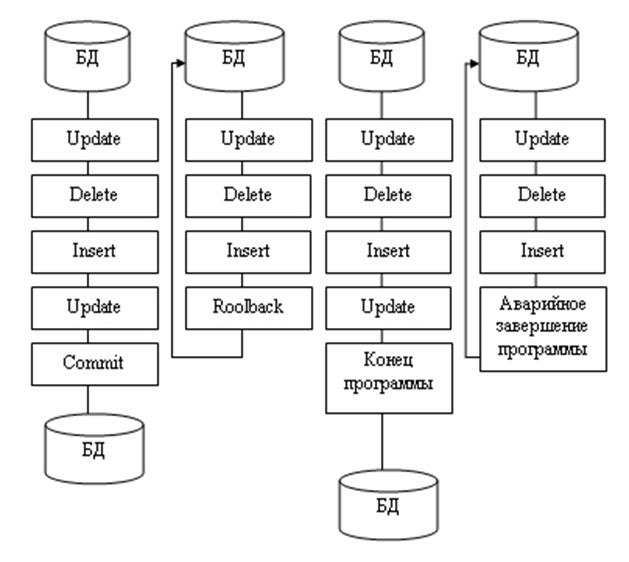
\includegraphics[width=0.8\textwidth]{assets/distributed/transactions.jpg}
    \caption{Модель транзакций ANSI/ISO}
	\label{ansi_transactions}
\end{figure}

Точки сохранения применяются, как правило, в протяженных транзакциях и позволяют разделить транзакцию на несколько
небольших осмысленных фрагментов. Пользователь может зафиксировать работу в любой точке транзакции с тем,
чтобы выполнить ее откат к состоянию, соответствующему этой точке.

Откат и фиксация транзакций становятся возможными благодаря журналу транзакций. Он используется следующим образом.
Известно, что все операции над реляционной базой данных суть операции над строками таблиц. Следовательно,
для обеспечения отката таблиц к предыдущим состояниям достаточно хранить не состояния таблицы, а лишь те
ее строки, которые подверглись изменениям.

При выполнении любого оператора SQL, который вносит изменения в базу данных, СУБД автоматически заносит
очередную запись в журнал транзакций. Запись состоит из двух компонентов: первый - это состояние строки до
внесения изменений, второй - ее же состояние после внесения изменений. Только после записи в журнал транзакций
СУБД действительно вносит изменения в базу данных. Если после данного оператора SQL был выполнен оператор
COMMIT, то в журнале транзакций делается отметка о завершении текущей транзакции. Если же после
оператора SQL следовал оператор ROLLBACK, то СУБД просматривает журнал транзакций и отыскивает записи,
отражающие состояние измененных строк до внесения изменений. Используя их, СУБД восстанавливает те
строки в таблицах базы данных, которые были изменены текущей транзакцией, - таким образом
аннулируются все изменения в базе данных.

\subsubsection{Мониторы обработки транзакций}~\\
Мониторы обработки транзакций (Transaction Processing Monitor - TPM), или мониторы
транзакций - программные системы, предназначенные для поддержки выполнения распределённых транзакций.
Они относятся к категории middleware, то есть к ПО, работающему между ОС и приложениями \autocite{TransactionMonitors}.

Это происходит следующим образом: клиент начинает транзакцию и обращается к TPM, который выдаёт ему
идентификатор транзакции и контекст транзакции. Затем клиент с помощью RPC обращается к серверу,
включая контекст в обращение. Сервер извлекает контекст, уведомляет TPM о том, что он (сервер) участвует
в транзакции, и обрабатывает запрос как обычно. Так коиент обращается ко всем необходимым серверам. 
Когда клиент достиг окончания транзакции, он уведомляет об этом TPM, и тот выполняет протокол двухфазного коммита
для всех серверов, участвовавших в транзакции. После завершения протокола TPM уведомляет об этом клиента (Рис. \ref{tpm_process}). \autocite{WebServices}

\begin{figure}[h!]
    \centering
    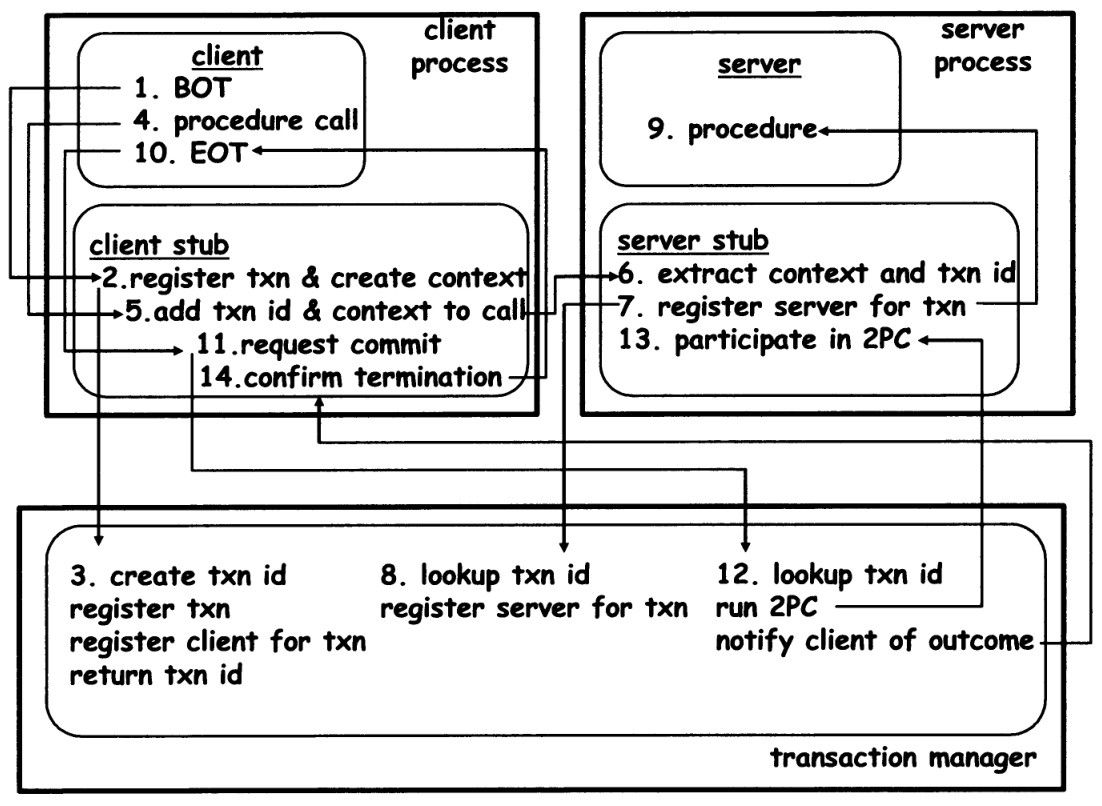
\includegraphics[width=0.8\textwidth]{assets/distributed/TPM_arch.png}
    \caption{Процесс взаимодействия с TPM}
	\label{tpm_process}
\end{figure}

TPM опираются на трехзвенную модель "клиент-сервер" (модель сервера приложений или AS-модель), описанную в Разделе 2.
Естественно, что все преимущества модели отражаются и на программных системах, построенных на ее основе.

На современном рынке мониторов транзакций основными "действующими лицами" являются такие системы,
как ACMS (DEC), CICS (IBM), TOP END (NCR), PATHWAY (Tandem), ENCINA (Transarc), TUXEDO System (USL).
Несмотря на принципиальное сходство, конкретные TPM отличаются рядом характеристик, причем
различия часто вытекают как из специфики операционной системы, в которой реализован и функционирует TPM.

\subsubsection{Корпоративная среда обработки транзакций}~\\

TPM на базе UNIX опирается на фундаментальное понятие - корпоративную среду обработки транзакций
(Enterprise Transaction Processing - ETP). Архитектура ETP - это три ряда компьютеров \autocite{TransactionMonitors}:
\begin{itemize}
    \item Ряд 1: Персональные станции (Personal Workstations);
    \item Ряд 2: Компьютеры под управлением ОС UNIX (UNIX Transaction Processing Servers - UPTS);
    \item Ряд 3: Mainframe-системы (Proprietary Transaction Processing Servers - PTPS)
    или компьютеры под управлением UNIX c RISC-архитектурой процессоров;
\end{itemize}

Компьютеры \textbf{ряда 1}, функционирующие под управлением DOS, MS Windows, OS/2, UNIX, используются в качестве рабочих мест
конечных пользователей. Характерная черта ETP - отсутствие ограничений на модели компьютеров,
составляющих этот ряд. Однако, как правило, ряд 1 состоит из компьютеров на базе процессоров Intel
486/Pentium под управлением MS Windows (MS Windows фактически стала стандартом оконного графического интерфейса
для большинства категорий пользователей и стандартом операционной среды для подавляющего числа прикладных программ и систем) \autocite{TransactionMonitors}.

\textbf{Ряд 2} составляют компьютеры среднего класса под управлением ОС UNIX,
на которых функционирует ядро TPM и, как правило, реляционные СУБД (Oracle, Informix, Ingres),
выступающие в качестве менеджера ресурсов. Кроме того, на них же может быть установлен шлюз к TPM в
операционной среде мэйнфрейма (как правило, разработчики TPM на базе UNIX предусматривают в конфигурации своих
систем шлюз к наиболее популярной такой системе - IBM CICS) \autocite{TransactionMonitors}.

\textbf{Ряд 3} представлен мэйнфреймами или RISC-компьютерами под управлением UNIX. О мэйнфреймах мы
говорим в тех ситуациях, когда исторически сложилось так, что в организации они существуют уже долгое время,
берут на себя большую часть всего объема обработки транзакций, концетрируют огромные вычислительные
ресурсы и содержат большие массивы данных (то есть речь идет об унаследованных системах). Если этого
"тяжелого наследия" нет, то можно смело использовать в качестве компьютеров ряда 3 RISC-серверы,
сегодня приближающиеся по производительности к мэйнфреймам \autocite{TransactionMonitors}.

Таким образом, среда обработки транзакций формируется из набора разнородных компьютеров (и соответствующих ОС),
ранжируемых от персональных компьютеров до мэйнфрейм-систем. TPM на базе UNIX представляет собой своего
рода "клей", который связывает вместе компьютеры трех рядов в открытую унифицированную среду обработки транзакций.

Ключом к интеграции систем, функционирующих на компьютерах различных рядов, является специализированный
интерфейс прикладного программирования ATMI (Application Transaction Manager Interface), обеспечивающий \autocite{TransactionMonitors}:
\begin{itemize}
    \item для ряда 1 - формирование и передачу запросов от клиентов к серверам, выполняющимся на компьютерах ряда 2
    \item для ряда 2 - обработку запросов, поступающих от компьютера ряда 1 (в том числе и с
    обращением к менеджеру ресурсов), и, по необходимости, формирование и направление
    запросов к серверам, выполняющимся на компьютерах ряда 3
    \item для ряда 3 - обработку запросов, поступающих от серверов ряда 2
\end{itemize}

Стоит отметить, что подобное представление о корпоративной среде обработки транзакций не является абстракцией.
Сегодня многие организации приходят именно к такой, "трехуровневой"  архитектуре информационных
систем (с той оговоркой, что наличие ряда 3 вызвано историческими причинами - мэйнфреймы использовались
первоначально и сразу от них отказаться невозможно).

\subsection{Протоколы фиксации}
\paragraph{Протоколы фиксации}~\\
Протоколы фиксации используются для обеспечения атомарности транзакций между сайтами.
Транзакция, которая выполняется на нескольких сайтах, должна быть либо зафиксирована на всех сайтах, либо прервана на всех сайтах.
Недопустимо, чтобы транзакция была зафиксирована на одном сайте и прервана на другом.
В локальной системе базы данных для принятия транзакции диспетчер транзакций должен только передать решение
о фиксации диспетчеру восстановления. Однако в распределенной системе диспетчер транзакций должен передать
решение о фиксации всем серверам в различных сайтах, где выполняется транзакция, и обеспечить
единообразное выполнение решения. Когда обработка завершается на каждом сайте, она достигает состояния
частично подтвержденной транзакции и ожидает, пока все другие транзакции достигнут их частично подтвержденных состояний.
Когда он получает сообщение о том, что все сайты готовы к фиксации, он начинает фиксировать.
В распределенной системе либо все сайты фиксируют, либо ни один из них не делает \autocite{FixProtocols}.

Различные протоколы распределенной фиксации \autocite{FixProtocols}:
\begin{itemize}
    \item Однофазный коммит
    \item Двухфазный коммит
    \item Трехфазный коммит
\end{itemize}
Широко используется протокол двухфазной фиксации (2PC).
\bigbreak
\subsubsection{Распределенная однофазная фиксация}

Распределенная однофазная фиксация – это самый простой протокол фиксации. Давайте рассмотрим, что есть
контролирующий сайт и несколько подчиненных сайтов, где выполняется транзакция. Шаги в распределенном коммите \autocite{FixProtocols}:
\begin{itemize}
    \item После того, как каждое ведомое устройство локально завершило свою транзакцию, оно
    отправляет сообщение «ГОТОВО» на контролирующий сайт
    \item Подчиненные ожидают сообщения «Подтвердить» или «Прервать» с контролирующего сайта.
    Это время ожидания называется окном уязвимости
    \item Когда контролирующий сайт получает сообщение «СДЕЛАНО» от каждого ведомого, он принимает решение
    о фиксации или отмене. Это называется точкой фиксации. Затем он отправляет это сообщение всем рабам
    \item При получении этого сообщения ведомое устройство либо фиксирует, либо прерывает работу,
    а затем отправляет подтверждающее сообщение на контролирующий сайт
\end{itemize}

После того, как каждое ведомое устройство локально завершило свою транзакцию, оно отправляет сообщение
«ГОТОВО» на контролирующий сайт.

Подчиненные ожидают сообщения «Подтвердить» или «Прервать» с контролирующего сайта. Это время ожидания
называется окном уязвимости.

Когда контролирующий сайт получает сообщение «СДЕЛАНО» от каждого ведомого, он принимает решение о
фиксации или отмене. Это называется точкой фиксации. Затем он отправляет это сообщение всем рабам.

При получении этого сообщения ведомое устройство либо фиксирует, либо прерывает работу,
а затем отправляет подтверждающее сообщение на контролирующий сайт.

\bigbreak
\subsubsection{Распределенная двухфазная фиксация}
Распределенная двухфазная фиксация снижает уязвимость однофазных протоколов фиксации. Шаги, выполняемые на двух этапах \autocite{FixProtocols}:
\bigbreak
\textbf{Этап 1}
\begin{itemize}
    \item После того, как каждое ведомое устройство локально завершило свою транзакцию,
    оно отправляет сообщение «ГОТОВО» на контролирующий сайт. Когда контролирующий сайт получил сообщение «ГОТОВО»
    от всех подчиненных, он отправляет сообщение «Подготовить» подчиненным
    \item Рабы голосуют за то, хотят ли они по-прежнему совершать или нет. Если ведомый
    хочет зафиксировать, он отправляет сообщение «Готово»
    \item Раб, который не хочет коммитить, отправляет сообщение «Не готов». Это может произойти,
    если ведомое устройство имеет конфликтующие параллельные транзакции или истекло время ожидания
\end{itemize}

После того, как каждое ведомое устройство локально завершило свою транзакцию, оно отправляет
сообщение «ГОТОВО» на контролирующий сайт. Когда контролирующий сайт получил сообщение «ГОТОВО» от всех подчиненных,
он отправляет сообщение «Подготовить» подчиненным.

Рабы голосуют за то, хотят ли они по-прежнему совершать или нет. Если ведомый хочет зафиксировать,
он отправляет сообщение «Готово».

Раб, который не хочет коммитить, отправляет сообщение «Не готов». Это может произойти, если ведомое
устройство имеет конфликтующие параллельные транзакции или истекло время ожидания.

\textbf{Этап 2}

\begin{itemize}
    \item После того, как контролирующий сайт получил сообщение «Готово» от всех ведомых \autocite{FixProtocols} –
    \begin{itemize}
        \item Контролирующий сайт отправляет сообщение «Global Commit» подчиненным
        \item Подчиненные устройства применяют транзакцию и отправляют сообщение «Подтвердить ACK» на контролирующий сайт
        \item Когда контролирующий сайт получает сообщение «Подтвердить ACK» от всех ведомых
        устройств, он считает транзакцию подтвержденной
    \end{itemize}
    \item После того, как контролирующий сайт получил первое сообщение «Не готов» от любого ведомого –
    \begin{itemize}
        \item Контролирующий сайт отправляет сообщение «Global Abort» подчиненным
        \item Слэйвы отменяют транзакцию и отправляют сообщение «Abort ACK» на контролирующий сайт
        \item Когда контролирующий сайт получает сообщение «Abort ACK» от всех ведомых
        устройств, он считает транзакцию отмененной
    \end{itemize}

\end{itemize}
\textbf{Обработка отказов}

Введём следующие обозначения: T -- транзакция, инициированная сайтом $S_i$, координатором которого выступает $C_i$.

\begin{itemize}
\item Отказ сайта

Когда сайт восстанавливается, он просматривает свой журнал, чтобы определить судьбу транзакций, активных во время сбоя\autocite{Fixations}:
\begin{itemize}
\item Журнал содержит запись <commit T>: сайт выполняет переотправку (T)
\item Журнал содержит запись <abort T>: сайт выполняет отмену (T)
\item Журнал содержит запись <ready T>: сайт должен обратиться к $C_i$, чтобы определить судьбу T.
\begin{itemize}
\item Если T зафиксировано, повторить (T)
\item Если Т прервано, отмена (Т).
\end{itemize}
\item Журнал не содержит никаких управляющих записей относительно ответов T что $S_k$ потерпел неудачу, прежде чем ответил на сообщение prepare T от $C_i$
\begin{itemize}
\item поскольку отказ $S_k$ исключает отправку такого ответа $C_1$ должен прервать T
\item $S_k$ должен выполнить отмену (T)
\end{itemize}
\end{itemize}  

\item Отказ координатора

Если координатор вышел из строя во время выполнения протокола фиксации для T то участвующие сайты должны принять решение о дальнейшей судьбе T\autocite{Fixations}:
\begin{itemize}
\item Если активный сайт содержит запись <commit T> в своем журнале, то T должен быть зафиксирован.
\item Если активный сайт содержит в своем журнале запись <abort T>, то T должен быть прерван.
\item Если какой-либо активный участвующий сайт не содержит записи <ready T> в своем журнале, тогда отказавший координатор $C_i$ не может принять решение о фиксации T. Поэтому можно прервать T.
\item Если ни один из вышеперечисленных случаев не подходит, то все активные сайты должны иметь запись <ready T> в своих журналах, но никаких дополнительных управляющих записей (таких как <abort T> из <commit T>). В этом случае активные сайты должны ждать, пока $C_i$ восстановится, чтобы найти решение.
\item Проблема блокировки: активным сайтам, возможно, придется ждать, пока вышедший из строя координатора будет восстановлен.
\end{itemize}
\item Разделение сети

Если координатор и все его участники остаются в одном разделе, отказ не влияет на протокол фиксации.\autocite{Fixations}
Если координатор и его участники принадлежат к нескольким разделам:
\begin{itemize}
\item Сайты, которые не находятся в разделе, содержащем координатора считают, что координатор вышел из строя, и выполняют протокол, соответствующий случаю отказа координатора.

\end{itemize}
Координатор и сайты, находящиеся в том же разделе, что и координатор считают, что сайты в другом разделе отказали, и следуют обычному протоколу фиксации.


\end{itemize}

\bigbreak
\textbf{Контролирование управления и параллелизма}

В случае обработки in-doubt (т.е. таких, о которых в логах есть запись <ready T>, но нет ни <commit T>, ни <abort T>) транзакций восстанавливающий сайт должен определить её commit-abort статус контактируя с другими сайтами, что может замедлить и, возможно, заблокировать процесс востановления\autocite{Fixations}.

Опишем основные принципы работы алгоритмов восстановления:
\begin{itemize}
    \item Алгоритмы могут записывать информацию о фиксациях в лог.
    \item Вместо <ready T> вносится запись <ready T, L>, где L -- список фиксаций, удерживаемых транзакцие T при записи лога, причём фиксации чтения могут быть опущены.
    \item Для каждой in-doubt транзакции T все фиксации, записанные в <ready T, L> запрашиваются снова.
    \item После повторного получения фиксации обработка транзакции может быть продолжена, при этом фиксация/откат in-doubt транзакции выполняется параллельно с исполнением новых транзакций.
\end{itemize}

\bigbreak
\subsubsection{Распределенная трехфазная фиксация}
Шаги в распределенной трехфазной фиксации следующие \autocite{FixProtocols}:
\begin{itemize}
    \item Этап 1: Шаги такие же, как при распределенной двухфазной фиксации
    \item Этап 2: Подготовьтесь к фиксации
    \begin{itemize}
        \item Контролирующий сайт выдает широковещательное сообщение «Ввод подготовленного состояния»
        \item Ведомые сайты голосуют «ОК» в ответ
    \end{itemize}
    \item Фиксация / Отмена
\end{itemize}

Этапы аналогичны двухфазной фиксации, за исключением того, что сообщение «Подтвердить ACK» / «Прервать ACK» не требуется

\subsubsection{Защищенные протоколы фиксации}
\paragraph{Обработка распределенных транзакций в базах данных с многоуровневой секретностью (MLS)}~\\
Известно, что в MLS/DBMS не ко всем данным, содержащимся в  базе
данных, доступ осуществляется одинаково. Однако современные СУБД, как
правило,  не имеют адекватных средств диагностики и механизма определения
того, что пользователь имеет возможность доступа только  к  тем
данным,  которые являются релевантными. Таким образом, MLS/DBMS отличается
от соответствующих DBMS,  по крайней  мере,  следующими  двумя
особенностями \autocite{SecureFix}:
\begin{itemize}
    \item каждый элемент данных в базе данных связан с уровнем доступа
    \item доступ пользователя к данным должен контролироваться релевантностью для данного пользователя
\end{itemize}
Разработка сервиса MLS/DBMS в современных компьютерных  системах
представляет  много  проблем. До настоящего времени внедрение многоуровневого
разграничения доступа в операционную  систему  представляет
собой  значительные трудности. Решение этой проблемы в виде аббревиатуры
обозначается ТСВ. Хотя в разрешении вопросов ТСВ  для  удаленных
пользователей  в  MLS/DBMS вводятся компромиссы, остается много проблем,
которые требуется разрешать. Наиболее очевидная проблема состоит
в том, что вопросы классификации в СУБД значительно  сложнее,  чем  в
файловых  системах  и могут быть сложнее реализованы. Другая проблема
состоит в том, что для классификации данных,  содержащих  контекстные
представления,  временные параметры, их композицию, необходимы унифицированные базы данных \autocite{SecureFix}.

\subsection{Тиражирование данных}
\textbf{Тиражирование данных} - это асинхронный перенос изменений объектов исходной базы данных (source database)
в базы данных, принадлежащие к различным узлам распределенной системы. Тиражирование данных может происходит
двумя различными способами: \textbf{шардингом} (или, иначе говоря, шардированием, фрагментацией) и \textbf{репликацией}.

\subsubsection{Шардинг (sharding)}

\textbf{Шардинг} — это метод проектирования базы данных, при котором данные разделяются на группы и хранятся на разных серверах. Это улучшает производительность, поскольку данные хранятся там, где они чаще всего используются, что уменьшает сетевой трафик.

Существуют два основных вида шардирования: \textbf{горизонтальное} и \textbf{вертикальное}. Они соответствуют операциям сокращения и проекции в реляционных базах данных. Важно, чтобы все фрагменты были независимыми, то есть ни один из фрагментов не может быть представлен как производный от других фрагментов.

Одной из ключевых особенностей шардинга является поддержка независимости от шардирования. Это означает, что пользователи могут работать так, как если бы данные в действительности были вовсе не шардированы. Это упрощает разработку пользовательских программ и выполнение терминальных операций.

Если обеспечивается независимость от шардирования, пользователи получают данные в виде представления, в котором шарды логически скомбинированы с помощью операций соединения и объединения. Задачей системного оптимизатора является определение шардов, к которым требуется доступ для выполнения запросов пользователя.
\autocite{IntroBD2014}

\paragraph{Алгоритмы шардинга} ~\\
Ранее уже упоминалось о двух основных вида шардинга: \textit{горизонтальный} и \textit{вертикальный}. Стоит их разобрать по подробнее и
рассказать и про другие виды шардирования, такие как шадинг на основе каталогов и шардинг на основе ключей.

\paragraph{Горизонтальное шардирование} ~\\
В этом методе мы разбиваем данные на основе диапазонов заданного значения, присущего каждой сущности. Допустим, у вас
есть база данных имен ваших онлайн-клиентов и информации об электронной почте. Вы можете разделить эту информацию на
два осколка. В одном осколке вы можете хранить информацию о клиентах, чье имя начинается с A-P, а в другом - информацию
об остальных клиентах.

\begin{figure}[H]
    \centering
    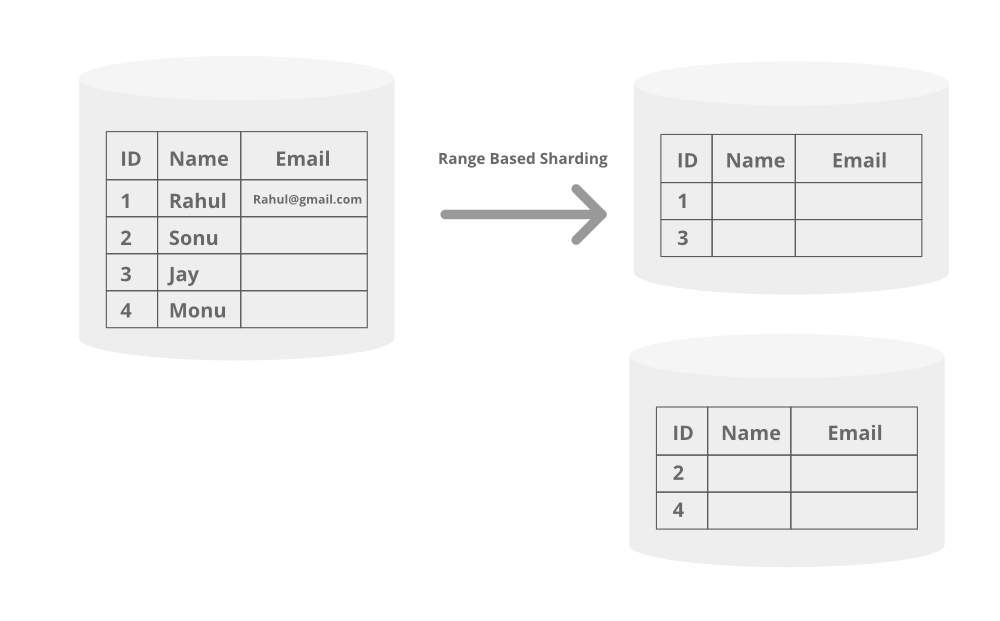
\includegraphics[width=100mm]{assets/distributed/Horizontal-Sharding}
    \caption{Горизонтальное шардирование}
    \label{fig:Horizontal-Sharding}
\end{figure}

\textbf{Горизонтальное шардирование} - самый простой метод сегментирования для реализации. Каждый осколок содержит
другой набор данных, но все они имеют ту же схему, что и исходная база данных. В этом методе вам просто нужно
определить, в какой диапазон попадают ваши данные, а затем вы можете сохранить запись в соответствующий шард. Этот
метод лучше всего подходит для хранения нестатических данных (например, хранение контактной информации студентов
колледжа).

Недостатком этого метода является то, что данные могут быть неравномерно распределены по шардам. В приведенном выше
примере у вас может быть много клиентов, имена которых попадают в категорию A-P. В таких случаях первый осколок должен
будет взять на себя больше нагрузки, чем второй, и это может стать узким местом системы. \autocite{DatabaseSharding}

\paragraph{Вертикальное шардирование} ~\\
В этом методе мы разделяем весь столбец из таблицы и помещаем эти столбцы в новые отдельные таблицы. Данные полностью
независимы от одного раздела к другому. Кроме того, каждый раздел содержит как отдельные строки, так и столбцы. Возьмем,
к примеру, функции Twitter. Мы можем разделить различные функции объекта на разные сегменты на разных машинах. В
Твиттере у пользователя может быть профиль, количество подписчиков и некоторые твиты, опубликованные им самим. Мы можем
разместить профили пользователей на одном осколке, подписчиков - на втором, а твиты - на третьем.

\begin{figure}[H]
    \centering
    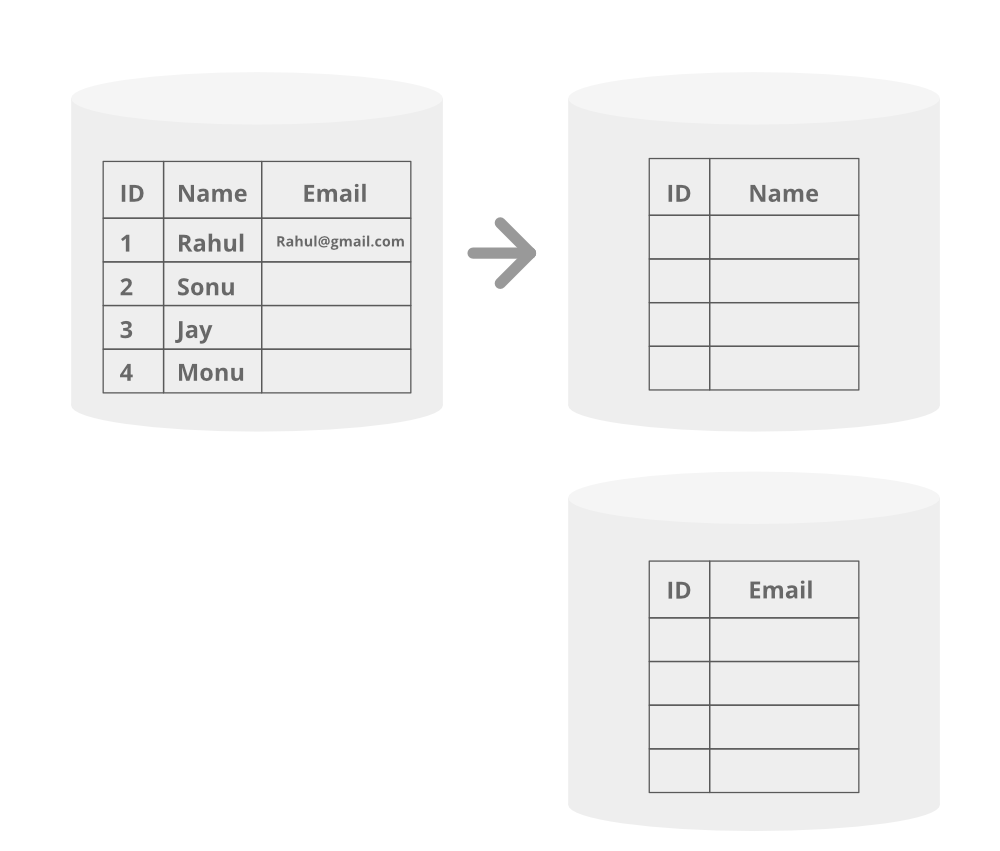
\includegraphics[width=100mm]{assets/distributed/Vertical-Sharding}
    \caption{Вертикальное шардирование}
    \label{fig:Vertical-Sharding}
\end{figure}

В этом методе вы можете отделить и обработать критическую часть (например, профили пользователей) от некритической части
ваших данных (например, сообщения в блоге) по отдельности и построить вокруг нее различные модели репликации и
согласованности. Это одно из главных преимуществ этого метода.

Основным недостатком этой схемы является то, что для ответа на некоторые запросы вам, возможно, придется комбинировать
данные из разных шардов, что неоправданно увеличивает сложность разработки и эксплуатации системы. Кроме того, если
ваше приложение будет расти позже, и вы добавите в него еще несколько функций, вам придется дополнительно сегментировать
базу данных с конкретными функциями на нескольких серверах. \autocite{DatabaseSharding}

\paragraph{Шардинг на основе каталогов} ~\\
В этом методе мы создаем и поддерживаем службу поиска или таблицу поиска для исходной базы данных. В основном мы
используем ключ осколка для таблицы поиска и делаем сопоставление для каждого объекта, существующего в базе данных.
Таким образом, мы отслеживаем, какие осколки базы данных содержат какие данные.

Таблица поиска содержит статический набор информации о том, где можно найти конкретные данные. На приведенном выше
изображении вы можете видеть, что мы использовали зону доставки в качестве ключа осколка. Во-первых, клиентское
приложение запрашивает службу поиска, чтобы узнать осколок (раздел базы данных), на котором размещены данные. Когда
служба поиска возвращает осколок, она запрашивает/обновляет этот осколок.

\begin{figure}[H]
    \centering
    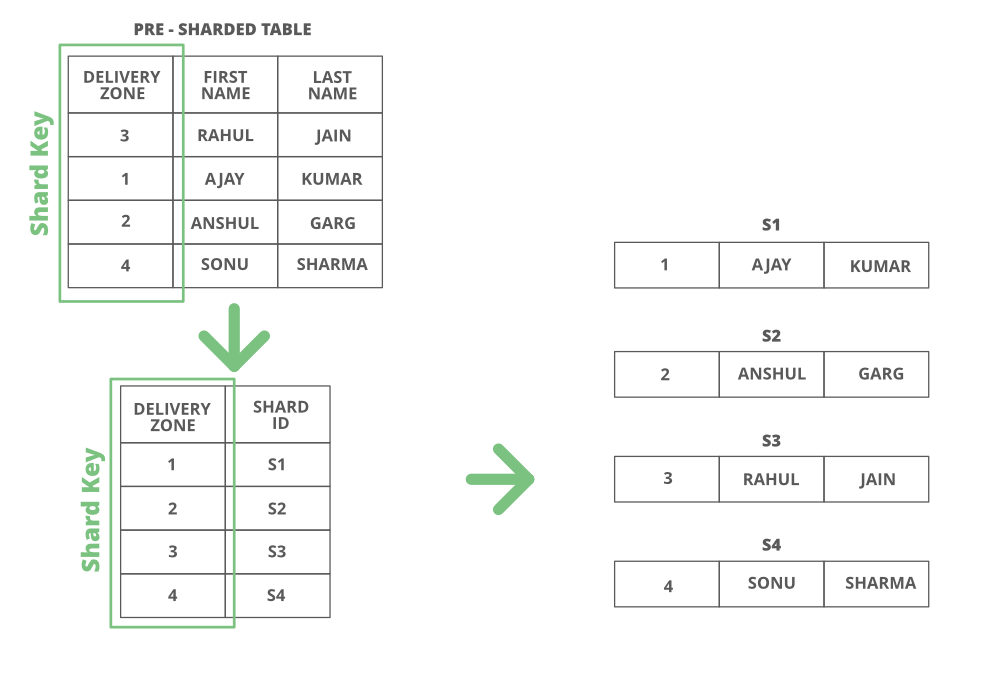
\includegraphics[width=100mm]{assets/distributed/Directory-Based-Sharding}
    \caption{Шардинг на основе каталогов}
    \label{fig:Directory-Based-Sharding}
\end{figure}

Сегментация на основе каталогов гораздо более гибкая, чем сегментация на основе диапазонов и ключей. В сегменте на
основе диапазонов вы обязаны указать диапазоны значений. В key-based вы обязаны использовать фиксированную хэш-функцию,
которую трудно изменить позже. При таком подходе вы можете использовать любой алгоритм, который хотите назначить для
записей данных в сегменты. Кроме того, при таком подходе легко динамически добавлять шарды.

Основным недостатком этого подхода является единственная точка отказа таблицы поиска. Если он будет поврежден или не
удался, это повлияет на запись новых данных или доступ к существующим данным из таблицы. \autocite{DatabaseSharding}

\paragraph{Шардинг на основе ключей} ~\\
Этот метод также известен как сегментация на основе хэша. Здесь мы берем значение объекта, такого как идентификатор
клиента, адрес электронной почты клиента, IP-адрес клиента, почтовый индекс и т. д., и мы используем это значение в
качестве входных данных хэш-функции. Этот процесс генерирует хэш-значение, которое используется для определения того,
какой шард нам нужно использовать для хранения данных. Мы должны иметь в виду, что значения, введенные в хэш-функцию,
должны поступать из одного и того же столбца (ключ осколка), чтобы данные размещались в правильном порядке и
согласованно. В принципе, ключи осколков действуют как первичный ключ или уникальный идентификатор для отдельных строк.

\begin{figure}[H]
    \centering
    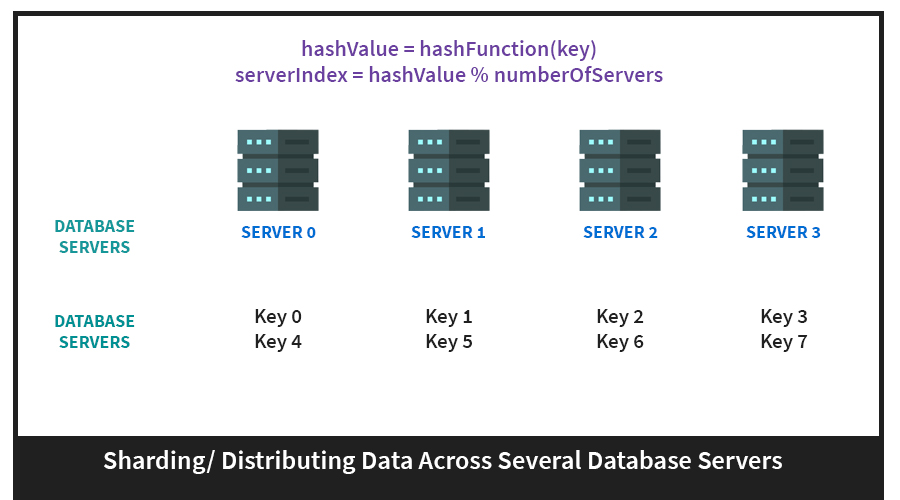
\includegraphics[width=100mm]{assets/distributed/Keybased-Sharding}
    \caption{Шардинг на основе ключей}
    \label{fig:Keybased-Sharding}
\end{figure}

Рассмотрим пример, что у вас есть 3 сервера баз данных, и каждый запрос имеет идентификатор приложения, который
увеличивается на 1 каждый раз, когда регистрируется новое приложение. Чтобы определить, на каком сервере должны быть
размещены данные, мы выполняем операцию по модулю для этих приложений id с номером 3. Затем остаток используется для
идентификации сервера для хранения наших данных.

Недостатком этого метода является эластичная балансировка нагрузки, что означает, если вы попытаетесь динамически
добавлять или удалять серверы баз данных, это будет сложный и дорогостоящий процесс. Например, в приведенном выше
примере, если вы добавите еще 5 серверов, вам нужно добавить больше соответствующих хэш-значений для дополнительных
записей. Кроме того, большинство существующих ключей необходимо переназначить на их новое, правильное хэш-значение,
а затем перенести на новый сервер. Хэш-функция должна быть изменена с модуля 3 на модуль 8. В то время как миграция
данных действует, как новые, так и старые хэш-функции не будут действительны. Во время миграции ваше приложение не
сможет обслуживать большое количество запросов, и вы будете испытывать простои для своего приложения до завершения
миграции. \autocite{DatabaseSharding}

\paragraph{Географический шардинг} ~\\
Шардирование по географическому признаку позволяет хранить определенные данные вблизи своих потребителей и
удовлетворять нормативным требованиям, когда данные должны находиться в определенной юрисдикции. Однако данный способ
шардирования не является самодостаточным: шарды могут быть загружены не равномерно, и отличие может быть на порядки.
На пример, экземпляр базы данных, хранящий данные пользователей Москвы и Московской области, будет намного превышать
другой экземпляр базы данных, который хранит информацию о пользователях из Владимира. Таким образом, недостатком
данного метода является необходимость дополнительного использования других методов шардирования.

\subsubsection{Репликация} ~\\
\textbf{Репликация} — это процесс изменения одного набора данных, называемого репликой, в ответ на изменения другого
набора данных, называемого основным. Репликация желательна по крайней мере по двум причинам. Во-первых, она способна
обеспечить более высокую производительность, поскольку приложения смогут обрабатывать локальные копии вместо того,
чтобы устанавливать связь с удаленными узлами. Во-вторых, наличие репликации может также обеспечивать более высокую
степень доступности, поскольку любой реплицируемый объект остается доступным для обработки (по крайней мере, для выборки
данных), пока хотя бы одна реплика в системе остается доступной. Главным недостатком репликации, безусловно, является
то, что если реплицируемый объект обновляется, то и все его копии должны быть обновлены (проблема распространения
обновлений).

Очевидно, что репликация, как и шардирование, теоретически должна быть "прозрачной для пользователя". Другими словами,
система, которая поддерживает репликацию данных, должна также поддерживать независимость от репликации (иногда говорят
"прозрачность репликации"). Для пользователей должна быть создана такая среда, чтобы они, по крайней мере, с логической
точки зрения могли считать, что в действительности данные не дублируются. Независимость от репликации (как и
независимость от шардирования) является весьма желательной, поскольку она упрощает создание пользовательских программ и
выполнение терминальных операций. В частности, независимость от репликации позволяет создавать и уничтожать дубликаты в
любой момент в соответствии с изменяющимися требованиями, не затрагивая при этом никакие из пользовательских программ
или терминальных операций.

Из требования независимости от репликации следует, что к обязанностям системного оптимизатора также относится
определение, какой именно из физических дубликатов будет применен для доступа к данным при выполнении каждого
введенного пользователем запроса. \autocite{IntroBD2014}

Можно выделить три \textbf{подхода к репликации}:
\begin{itemize}
    \item Блочная репликация на уровне системы хранения данных;
    \item Физическая репликация на уровне СУБД;
    \item Логическая репликация на уровне СУБД.
\end{itemize}

\paragraph{Блочная репликация} ~\\
При блочной репликации каждая операция записи выполняется не только на основном диске, но и на резервном. Таким образом
тому на одном массиве соответствует зеркальный том на другом массиве, с точностью до байта повторяющий основной том.

К достоинствам такой репликации можно отнести простоту настройки и надёжность. Записывать данные на удалённый диск может
либо дисковый массив, либо нечто (устройство или программное обеспечение), стоящее между хостом и диском. Если дисковый
массив не способен реплицировать данные, между хостом и массивом может быть установлен агент, осуществляющей запись на
два массива сразу. Агент может быть как отдельным устройством, так и программным компонентом. В отличие от дискового
массива, который может работать только с таким же массивом или, как минимум, с массивом того же производителя, агент
может работать с совершенно разными дисковыми устройствами.

Главное назначение блочной репликации – обеспечение отказоустойчивости. Если база данных потеряна, то можно
перезапустить её с использованием зеркального тома. Блочная репликация хороша своей универсальностью, но за
универсальность приходится платить.

Во-первых, никакой сервер не может работать с зеркальным томом, поскольку его операционная система не может управлять
записью на него; с точки зрения наблюдателя данные на зеркальном томе появляются сами собой. В случае аварии (отказ
основного сервера или всего ЦОДа, где находится основной сервер) следует остановить репликацию, размонтировать основной
том и смонтировать зеркальный том. Как только появится возможность, следует перезапустить репликацию в обратном
направлении.

Во-вторых, сама СУБД на резервном сервере может быть запущена только после монтирования диска. В некоторых операционных
системах, например, в Solaris, память под кеш при выделении размечается, и время разметки пропорционально объёму
выделяемой памяти, то есть старт экземпляра будет отнюдь не мгновенным. Плюс ко всему кеш после рестарта будет пуст.

В-третьих, после запуска на резервном сервере СУБД обнаружит, что данные на диске неконсистентны, и нужно потратить
значительное время на восстановление с применением журналов повторного выполнения: сначала повторить те транзакции,
результаты которых сохранились в журнале, но не успели сохраниться в файлы данных, а потом откатить транзакции, которые
к моменту сбоя не успели завершиться. \autocite{Replication}

\paragraph{Физическая репликация (master-slave)} ~\\
Журналы (redo log или write-ahead log) содержат все изменения, которые вносятся в файлы базы данных. Идея физической
репликации состоит в том, что изменения из журналов повторно выполняются в другой базе (реплике), и таким образом данные
в реплике повторяют данные в основной базе байт-в-байт \autocite{PhysLogPeplic}.

Журналы СУБД не предназначены для использования вне этой платформы, их формат не документируется и может меняться без
предупреждения. Отсюда совершенно естественное требование, что физическая репликация возможна только между экземплярами
одной и той же версии одной той же СУБД. Отсюда же возможные ограничения на операционную систему и архитектуру
процессора, которые тоже могут влиять на формат журнала.

Естественно, никаких ограничений на модели СХД физическая репликация не накладывает. Более того, файлы в базе-реплике
могут располагаться совсем по-другому, чем на базе-источнике – надо лишь описать соответствие между томами, на которых
лежат эти файлы.

Запись данных в реплику невозможна, поскольку изменения в неё приходят побайтно, и реплика не может обеспечить
конкурентное исполнение своих запросов. В случае повреждения файла в основной базе можно просто скопировать
соответствующий файл с реплики. Однако стоит учесть, что файл на реплике может быть не идентичен файлу в основной базе:
когда файл расширяется, новые блоки в целях ускорения ничем не заполняются, и их содержимое случайно. База может
использовать не всё пространство блока (например, в блоке может оставаться свободное место), но содержимое
использованного пространства совпадает с точностью до байта \autocite{PhysLogPeplic}.

Физическая репликация может быть как синхронной, так и асинхронной. При асинхронной репликации всегда есть некий набор
транзакций, которые завершены на основной базе, но ещё не дошли до резервной, и в случае перехода на резервную базу при
сбое основной эти транзакции будут потеряны. При синхронной репликации завершение операции commit означает, что все
журнальные записи, относящиеся к данной транзакции, переданы на реплику. Важно понимать, что получение репликой журнала
не означает применения изменений к данным. При потере основной базы транзакции не будут потеряны, но если приложение
пишет данные в основную базу и считывает их из реплики, то у него есть шанс получить старую версию этих данных \autocite{PhysLogPeplic}.

Физическая репликация базы данных имеет множество преимуществ перед репликацией средствами СХД \autocite{PhysLogPeplic}:
\begin{itemize}
    \item объём передаваемых данных меньше за счёт того, что передаются только журналы, но не файлы с данными; эксперименты показывают уменьшение трафика в 5-7 раз;
    \item переключение на резервную базу происходит значительно быстрее: экземпляр-реплика уже поднят, поэтому при переключении ему нужно лишь откатить активные транзакции; более того, к моменту сбоя кеш реплики уже прогрет;
    \item на реплике можно выполнять запросы, сняв тем самым часть нагрузки с основной базы. В частности, реплику можно использовать для создания резервных копий.
\end{itemize}

\paragraph{Логическая репликация (active-active)} ~\\
Все изменения в базе данных происходят в результате вызовов её API – например, в результате выполнения SQL-запросов.
Очень заманчивой кажется идея выполнять одну и ту же последовательность запросов на двух разных базах. Для репликации
необходимо придерживаться двух правил \autocite{PhysLogPeplic}:
\begin{itemize}
    \item нельзя начинать транзакцию, пока не завершены все транзакции, которые должны закончиться раньше; Так на рисунке ниже нельзя запускать транзакцию D, пока не завершены транзакции A и B;
    \item нельзя завершать транзакцию, пока не начаты все транзакции, которые должны закончиться до завершения текущей транзакции; Так на рисунке ниже даже если транзакция B выполнилась мгновенно, завершить её можно только после того, как начнётся транзакция C.
\end{itemize}

\begin{figure}[H]
    \centering
    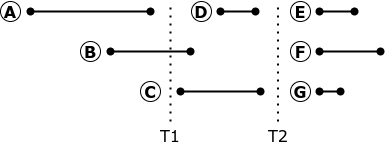
\includegraphics[width=100mm]{assets/distributed/ReplicationExample}
    \caption{Пример репликации}
    \label{fig:ReplicationExample}
\end{figure}

\textbf{Репликация команд (statement-based replication)} реализована, например, в MySQL. К сожалению, эта простая схема не
приводит к появлению идентичных наборов данных – тому есть две причины \autocite{PhysLogPeplic}.
\begin{itemize}
    \item не все API детерминированы. Например, если в SQL-запросе встречается функция now() или sysdate(), возвращающая текущее время, то на разных серверах она вернёт разный результат – из-за того, что запросы выполняются не одновременно. Кроме того, к различиям могут привести разные состояния триггеров и хранимых функций, разные национальные настройки, влияющие на порядок сортировки, и многое другое.
    \item репликацию, основанную на параллельном исполнении команд, невозможно корректно приостановить и перезапустить. На рисунке выше если репликация остановлена в момент T1 транзакция B должна быть прервана и откачена. При перезапуске репликации исполнение транзакции B может привести реплику к состоянию, отличному от состояния базы-источника: на источнике транзакция B началась до того, как закончилась транзакция A, а значит, она не видела изменений, сделанных транзакцией A. Репликация запросов может быть остановлена и перезапущена только в момент T2, когда в базе нет ни одной активной транзакции. Разумеется, на сколько-нибудь нагруженной промышленной базе таких моментов не бывает.
\end{itemize}

Обычно для логической репликации используют детерминированные запросы. Детерминированность запроса обеспечивается двумя
свойствами:
\begin{itemize}
    \item запрос обновляет (или вставляет, или удаляет) единственную запись, идентифицируя её по первичному (или уникальному) ключу;
    \item все параметры запроса явно заданы в самом запросе.
\end{itemize}

В отличие от \textbf{репликации команд (statement-based replication)} такой подход называется \textbf{репликацией
записей (row-based replication)} \autocite{PhysLogPeplic}.

База-реплика открыта и доступна не только на чтение, но и на запись. Это позволяет использовать реплику для выполнения
части запросов, в том числе для построения отчётов, требующих создания дополнительных таблиц или индексов. Важно
понимать, что логическая реплика будет эквивалентна исходной базе только в том случае, если в неё не вносится никаких
дополнительных изменений

Логическая репликация предоставляет ряд возможностей, отсутствующих в других видах репликации \autocite{PhysLogPeplic}:
\begin{itemize}
    \item настройка набора реплицируемых данных на уровне таблиц (при физической репликации – на уровне файлов и табличных пространств, при блочной репликации – на уровне томов);
    \item построение сложных топологий репликации – например, консолидация нескольких баз в одной или двунаправленная репликация;
    \item уменьшение объёма передаваемых данных;
    \item репликация между разными версиями СУБД или даже между СУБД разных производителей;
    \item обработка данных при репликации, в том числе изменение структуры, обогащение, сохранение истории.
\end{itemize}

Есть и недостатки, которые не позволяют логической репликации вытеснить физическую \autocite{PhysLogPeplic}:
\begin{itemize}
    \item все реплицируемые данные обязаны иметь первичные ключи;
    \item логическая репликация поддерживает не все типы данных;
    \item логическая репликация на практике не бывает полностью синхронной: время от получения изменений до их применения слишком велико, чтобы основная база могла ждать;
    \item логическая репликация создаёт большую нагрузку на реплику;
    \item при переключении приложение должно иметь возможность убедиться, что все изменения с основной базы, применены на реплике – СУБД зачастую сама не может этого определить, так как для неё режимы реплики и основной базы эквивалентны.
\end{itemize}

Два последних недостатка существенно ограничивают использование логической реплики как средства отказоустойчивости. Если
один запрос в основной базе изменяет сразу много строк, реплика может существенно отставать. А возможность смены ролей
требует недюжинных усилий как со стороны разработчиков, так и со стороны администраторов.

Есть несколько способов реализации логической репликации, и каждый из этих способов реализует одну часть возможностей и
не реализует другую \autocite{PhysLogPeplic}:
\begin{itemize}
    \item репликация триггерами;
    \item использование журналов СУБД;
    \item использование программного обеспечения класса CDC (change data capture);
    \item прикладная репликация.
\end{itemize}

\paragraph{Репликация триггерами} ~\\
Триггер – хранимая процедура, которая исполняется автоматически при каком-либо действии по модификации данных. Триггеру,
который вызывается при изменении каждой записи, доступны ключ этой записи, а также старые и новые значения полей. При
необходимости триггер может сохранять новые значения строк в специальную таблицу, откуда специальный процесс на стороне
реплики будет их вычитывать

\textbf{Преимущества}:
\begin{itemize}
    \item независимость от версий основной базы и реплики;
    \item широкие возможности преобразования данных.
\end{itemize}

\textbf{Недостатки}:
\begin{itemize}
    \item нагрузка на основную базу;
    \item большая задержка при репликации.
\end{itemize}

\paragraph{Использование журналов СУБД} ~\\
Сами СУБД также могут предоставлять возможности логической репликации. Источником данных, как и для физической
репликации, являются журналы. К информации о побайтовом изменении добавляется также информация об изменённых полях, а
также значение уникального ключа, даже если он не меняется. В результате объём журналов БД увеличивается – по разным
оценкам от 10 до 15%.

К \textbf{недостаткам} данного подхода можно отнести увеличение объёма журналов и возможное увеличение трафика между
узлами.

\paragraph{Использование CDC} ~\\
Существует целый класс программного обеспечения, предназначенного для организации логической репликации. Это ПО
называется CDC, change data capture. В задачу платформы входит чтение журналов базы данных, преобразование информации,
передача информации на реплику и применение. Как и в случае репликации средствами самой СУБД, журнал должен содержать
информацию об изменённых полях. Использование дополнительного приложения позволяет «на лету» выполнять сложные
преобразования реплицируемых данных и строить достаточно сложные топологии репликации.

\textbf{Преимущества}:
\begin{itemize}
    \item возможность репликации между разными СУБД, в том числе загрузка данных в отчётные системы;
    \item широчайшие возможности обработки и преобразования данных;
    \item минимальный трафик между узлами – платформа отсекает ненужные данные и может сжимать трафик;
    \item встроенные возможности мониторинга состояния репликации.
\end{itemize}

\textbf{Недостатки}:
\begin{itemize}
    \item увеличение объёма журналов, как при логической репликации средствами СУБД;
    \item новое ПО – сложное в настройке и/или с дорогими лицензиями.
\end{itemize}

\paragraph{Прикладная репликация} ~\\
Наконец, ещё один способ репликации – формирование векторов изменений непосредственно на стороне клиента. Клиент должен
формировать детерминированные запросы, затрагивающие единственную запись. Добиться этого можно, используя специальную
библиотеку работы с базой данных. Когда приложение завершает транзакцию, специально подключаемый модуль записывает
вектор изменений в очередь и выполняет транзакцию в базе данных. Специальный процесс-репликатор вычитывает векторы из
очереди и выполняет транзакции в базе-реплике.Этот механизм хорош для обновления отчётных систем. Может он
использоваться и для обеспечения отказоустойчивости, но в этом случае в приложении должен быть реализован контроль
состояния репликации

\textbf{Преимущества}:
\begin{itemize}
    \item возможность репликации между разными СУБД, в том числе загрузка данных в отчётные системы;
    \item возможность обработки и преобразования данных, мониторинга состояния и т. д.;
    \item минимальный трафик между узлами – платформа отсекает ненужные данные и может сжимать трафик;
    \item полная независимость от базы данных – как от формата, так и от внутренних механизмов.
\end{itemize}

\textbf{Недостатки}:
\begin{itemize}
    \item ограничения на архитектуру приложения;
    \item огромный объём собственного кода, обеспечивающего репликацию.
\end{itemize}

\paragraph{Сравнение подходов к репликации} ~\\
Описав все подходы к репликации, можно установить следующее:
\begin{itemize}
    \item \textbf{Блочная репликация} имеет смысл, когда других способов репликации нет; для баз данных её лучше не использовать.
    \item \textbf{Физическая репликация} хороша, когда требуется обеспечение отказоустойчивости инфраструктуры или перенос части читающих приложений на реплики.
    \item \textbf{Логическая репликация} подходит для обеспечения отказоустойчивости только в том случае, если приложение знает об этой репликации и умеет в случае аварии ждать синхронизации реплик.
    \item \textbf{Логическая репликация} идеальна для всевозможных отчётных баз.
    \item \textbf{Репликация триггерами} имеет смысл в том случае, если база сильно нагружена, а реплицировать нужно крайне ограниченное количество информации.
    \item \textbf{Платформы CDC} хороши, если у вас большое количество реплицируемых баз и/или есть необходимость сложных преобразований данных.
    \item Разработка \textbf{прикладной репликации} оправдана только в случае разработки собственной платформы или фреймворка.
\end{itemize} \autocite{Replication}

\paragraph{Greenplum} ~\\
Ранее уже сравнивались различные подходы шардирования между собой. Сравнивались различные подходы репликации между
собой. Осталось только сравнить способы тиражирования, то есть сравнить репликацию и шардирование.

Вообще говоря, шардинг и репликация не противоречат друг другу и могут сосуществовать. Они выполняют разные задачи, и
сравнивать их не имеет смысла. Репликация используется для ускорения взаимодействия с бд с помощью использования копий
основной базы данных. Кроме того, репликация осуществляет отказоустойчивость. В свою очередь шардинг осуществляет
ускорение работы с базой данных с помощью разбиения исходной базы данных на несколько разных, хранящихся на разных
серверах.  Шардирование не реализует отказоустойчивость.

В принципе, на этом их сравнение можно закончить и перейти к примеру. Один из классических примеров в котором
реализовано сочетание репликации и шардирования - \textbf{Greenplum}.

\textbf{Greenplum (GP)} – реляционная СУБД, имеющая массово-параллельную (massive parallel processing) архитектуру без
разделения ресурсов (Shared Nothing). В общем случае кластер GP состоит из нескольких серверов-сегментов (именно
сегменты непосредственно хранят данные, выполняют с ними операции и отдают результаты мастеру (в общем случае). По сути
сегмент – самый обычный инстанс PostgreSQL 8.2.15 с настроенной логической репликацией в своё зеркало на другом
сервере), одного сервера-мастера (сервер, на котором работает инстанс, являющийся одновременно координатором и входной
точкой для пользователей в кластере), и одного сервера-секондари-мастера (инстанс, являющийся резервным мастером,
включается в работу в случае недоступности основного мастера (переключение происходит вручную)), соединённых между
собой одной или несколькими быстрыми (10g, infiniband) сетями, обычно обособленными (interconnect). На рисунке ниже
представлен состав кластера и сетевое взаимодействие элементов. Здесь — зелёная и красная линии — обособленные сети
interconnect, синяя линия — внешняя, клиентская сеть \autocite{Greenplum}.

\begin{figure}[H]
    \centering
    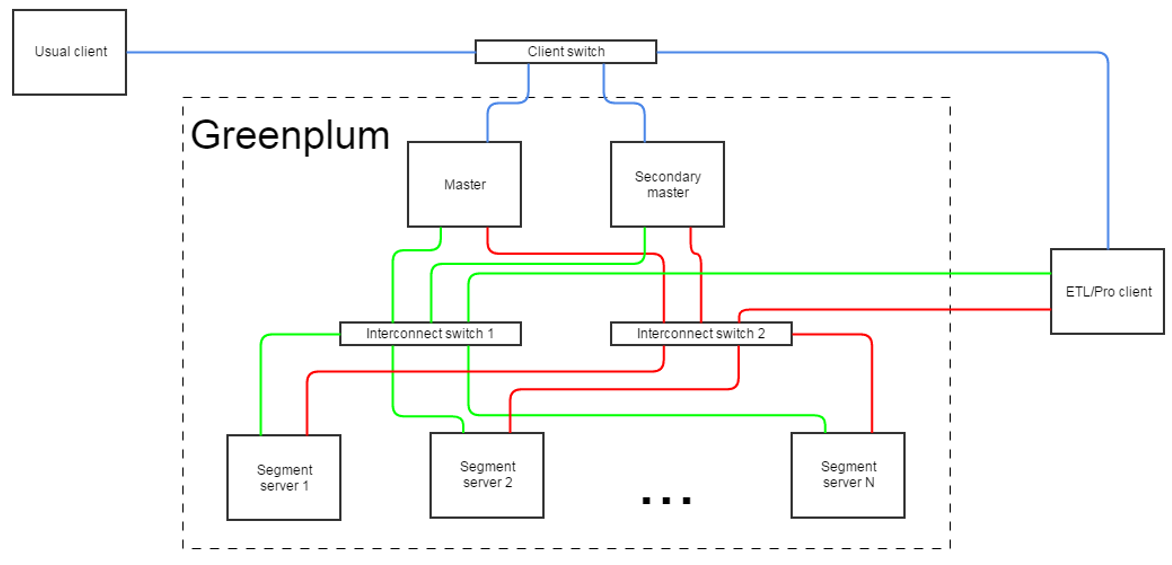
\includegraphics[width=100mm]{assets/distributed/Greenplum}
    \caption{Состав кластера и сетевое взаимодействие элементов Greenplum}
    \label{fig:Greenplum}
\end{figure}

При выборе числа серверов-сегментов важно правильно выбрать соотношение кластера «число процессоров/Тб данных» в
зависимости от планируемого профиля нагрузки на БД — чем больше процессорных ядер приходится на единицу данных, тем
быстрее кластер будет выполнять «тяжёлые» операции, а также работать со сжатыми таблицами.

При выборе числа сегментов в кластере (которое в общем случае к числу серверов никак не привязано) необходимо помнить
следующее \autocite{Greenplum}:
\begin{itemize}
    \item все ресурсы сервера делятся между всеми сегментами на сервере (нагрузкой зеркал, в случае если они располагаются на этих же серверах, можно условно пренебречь);
    \item каждый запрос на одном сегменте не может потреблять процессорных ресурсов больше, чем одно ядро CPU. Это означает, например, что, если кластер состоит из 32-ядерных серверов с 4-я сегментами GP на борту и используется в среднем для обработки 3-4 одновременных тяжёлых, хорошо утилизирующих CPU, запросов, «в среднем по больнице» CPU не будет утилизироваться оптимально. В данной ситуации лучше увеличить число сегментов на сервере до 6-8;
    \item штатный процесс бекапа и рестора данных «из коробки» работает только на кластерах, имеющих одинаковое число сегментов. Восстановить данные, забекапленные на кластере из 96 сегментов, в кластер из 100 сегментов без напильника будет невозможно.
\end{itemize}

В Greenplum реализуется классическая схема шардирования данных. Каждая таблица представляет из себя N+1 таблиц на всех
сегментах кластера, где N – число сегментов (+1 в этом случае — это таблица на мастере, данных в ней нет). На каждом
сегменте хранится 1/N строк таблицы. Логика разбиения таблицы на сегменты задаётся ключом (полем) дистрибуции – таким
полем, на основе данных которого любую строку можно отнести к одному из сегментов \autocite{Greenplum}.

По подробнее почитать про Greenplum можно в источнике. В данной главе приведена только краткая информация об общей
архитектуре и информация, относящаяся к тиражированию данных. \autocite{Greenplum}

\subsection{Бесконфликтные реплицированные типы данных}
\paragraph{Проблема репликации}
Предположим, реплики СУБД распределены по географическому признаку для ускорения работы приложения. А теперь пусть в разных репликах практически одновременно и независимо была изменена одна и та же строка. Какую строку считать правильно отражающей данные? Как восстановить согласованность между репликами? В общем случае, проблема одновременного обновления реплик не может быть разрешима. Поэтому большинство распределенных СУБД запрещают производить такие операции, например используя только один сервер для выполнения запросов. Однако существует некоторый класс структур данных, которые позволяют автоматически разрешать конфликты возникающие в процессе обновления нескольких реплик. Этот класс называется - бесконфликтные реплицированные типы данных или conflict-free replicated data types(CRDT). 
\paragraph{CRDT. Опеределение и виды}
CRDT обладают следующими характеристиками:
\begin{itemize}
    \item Приложение может обновлять реплики независимо, параллельно с другими репликами
    \item Алгоритм(как часть CRDT) автоматически разрешает возможные конфликты
    \item Данные в разных репликах могут быть в различных состояниях в один и тот же момент времени, но они гарантированно сойдутся спустя некоторое время 
\end{itemize}
Просто используя специализированные структуры данных было бы сложно добиться бесконфликтности, поэтому для ее достижения используются также специальные алгоритмы обновления данных. Алгоритмы определяют требования к структурам данных, а также могут накладывать дополнительные требования на сети передачи данных. Рассмотрим два основных вида алгоритмов:
\begin{itemize}
    \item Operation-based CRDTs. При обновлении данных, на реплике генерируется специальная функция обновления, которая затем рассылается всем другим нодам в сети. Каждая нода применяет эту функцию к своим данным и таким образом достигается консистентность. Важно, чтобы каждая функция была лишь раз применена на каждой ноде. Поэтому необходимо следить за тем, чтобы доставка гарантированно произошла и произошла только один раз. Связано это с тем, что функции могут быть коммутативными, но далеко не факт, что они будут идемпотентными(применение несколько раз подряд дает разные результаты).
    \item State-based CRDTs. При обновлении данных, репликам посылается полная локальная копия данных, после чего реплики локально у себя сливают эти изменения воедино, причем операция слияния (merge) обладает свойствами ассоциативности, коммутативности и идемпотентности, что позволяет уменьшить требования к каналам связи между репликами. 
    \item Delta-state CRDTs - оптимизированный вариант state-based CRDTs, когда посылаются только недавно примененные изменения вместо полной копии состояния.
\end{itemize}
Помимо алгоритмов, важную роль играют процессы сходимости между нодами. Для сходимости в случае Operation-based CRDTs, каждая нода обязана получить ровно одно сообщение с фукнцией обновления и для этого необходим надежный протокол доставки. В случае с State-base CRDTs, наличие коммутативного и идемпотентного оператора слияния позволяет утверждать, что данные постепенно сойдутся в любом случае, что дает нам право не беспокоиться о протоколе доставки. 
\paragraph{Примеры реализации}
На сегодняшний день известных CRDT не так много, одни из них: G-Counter (Grow only counter), PN-Counter (positive-negative counter), G-Set (grow only set) и несколько других типов. Основной особенностью всех этих типов данных является, то что каждая коллекция поддерживает узкий набор операций. А чтобы добавить например вычитание (некоммутативную операцию) в PN-Counter необходимо прибегать к хитрости и использовать два ворастающих счетчика типа G-Counter. Рассмотрим пример реалиции G-Counter-а. 
\begin{figure}[H]
    \centering
    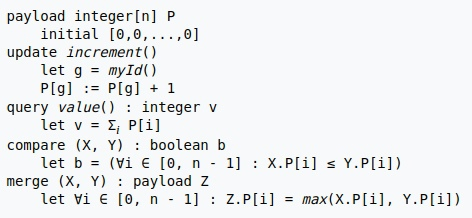
\includegraphics[width=100mm]{assets/distributed/G-Counter}
    \caption{Пример реализации Grow only Counter-а}
    \label{fig:G-Counter}
\end{figure}
Этот State-based счетчик сделан для кластера из n нод. Каждой ноде присвоен id, который можно получить вызвав функцию myid(). Таким образом, каждой ноде присваивается свой слот в массиве P, который нода может инкрементировать локально. Обновления расходятся по сети и при слиянии вычисляется максимум для каждого слота. При запросе значения счетчика все значения в слотах вектора суммируются и возвращаются в качестве ответа. Функция слияния является идемпотентной и коммутативной, поэтому данный счетчик является state-based.
Использование CRDT позволяет существенно упростить жизнь для разработчиков СУБД и облегчить работу с репликами. Уже сейчас CRDT используется во многих крупных проектах. В их число входит: Redis, Riak, Apple, Facebook. В дальнейшем использование CRDT будет только увеличиваться. 

\subsection{Интеграция БД и Internet}
\paragraph{Современные тенденции}
Заключаются в том, чтоб забыть о физических машинках и виртуалках, завернуть сервисы в контейнеры и перенести их в облако. Это позволяет разработчикам и компаниям быть более гибкими, 
упрощает разработку, тестирование и масштабирование приложений.

\subsubsection{Контейнеризация}

\textbf{Контейнеризация} обеспечивает ряд преимуществ:

\begin{itemize}
\item \textbf{Изоляция:} Каждый контейнер представляет собой изолированную среду, 
что позволяет приложениям работать независимо друг от друга, 
не влияя на другие приложения или систему.
\item \textbf{Портативность:} Контейнеры можно легко переносить между различными 
средами, будь то локальные машины, виртуальные машины или облачные платформы.
\item \textbf{Масштабируемость:} Контейнеры можно легко масштабировать 
вверх или вниз в зависимости от потребностей приложения.
\item \textbf{Эффективность:} Контейнеры используют меньше ресурсов, чем виртуальные машины, 
что делает их более экономичными.
\end{itemize}

\paragraph{Docker} ~\\

    Docker~--- средство виртуализации и менеджмента программ (сервисов), позволяющее гибко настраивать инфраструктуру проектов, и кратно облегчающее разработку, тестирование и масштабируемый деплой.
    Архитектура у Docker клиент-серверная, что означает наличие демона dockerd и клиентов docker, отправляющих демону команды (собери, скачай, запусти, пр.). Если вам нужно на коленке запустить оркестрацию
    (операции ``возьми n нод, запусти на них k заданий (образов Docker) и проследи, чтоб выполнились''), можно использовать docker swarm. \autocite{DockerSwarmConcepts} В проде такое лучше не использовать,
    потому что ноды приходится создавать ручками; иными словами, если у вас есть 2 машинки с разным количеством ресурсов каждая, придётся собственными силами подстраивать количество запускаемых на машинке нод,
    подстраиваясь под потребляемые ресурсы. Если требуется динамическое масштабирование, лучше посмотреть в сторону K8s.

    \textbf{Контейнеры} ~\\
    Основная идея~--- завернуть необходимый сервис (бинарники, скрипты, данные, конфиги) в легковесный \textbf{контейнер}, который далее будет запускаться на произвольном устройстве, способном запускать
    64-битный Linux (Windows и macOS под капотом запускают сначала виртуалку с Linux, и лишь на ней крутят Docker). Такой подход с упаковкой всего необходимого в контейнер позволяет не волноваться о том,
    что на хосте (устройство, где контейнер запущен) будет недоставать пакетов, возникнут проблемы с совместимостью и тому подобное.

    \textbf{Изолированность} ~\\
	Контейнеризация основана на технологии LXC (Linux Containers), 
	которая позволяет создавать изолированные среды внутри Linux-системы. 
	Каждый контейнер имеет собственную файловую систему, сетевой стек 
	и процессы, что обеспечивает его полную изоляцию от других контейнеров 
	и базовой системы. Процессы, запущенные в одном контейнере не смогут влиять и даже смотреть на то, что запущенно в другом контейнере или на хосте, а для получения таковой функциональности придётся приложить дополнительные усилия. 
    Обеспечивается такая изоляция средствами ядра Linux, а именно~--- \textbf{пространствами имён} (namespaces) и \textbf{контрольными группами} (control group). Первые отвечают за то, чтоб котнейнеры
    не подглядывали друг за другом; а вторые распределяют и ограничивают используемые контейнерами ресурсы хоста, гарантируют не только то, что контейнеры не будут голодать по памяти, CPU, дисковым операциям,
    но и то, что контейнеры не отберут все ресурсы у других потребителей.

    \textbf{Атаки на dockerd} ~\\
    Демон dockerd по умолчанию (можно запустить и в rootless режиме) требует root привилегий. Например, это требуется для пробрасывания директории хоста в контейнер. В связи с чем следует предоставлять
    управление демоном только тем пользователям, которым доверяешь. В пример можно привести атаку, в ходе которой корень файловой системы хоста примонтируется в директорию внутри контейнера, к которой
    у постороннего пользователя будет доступ. Для защиты от этого Docker использует не TCP сокеты, а UNIX сокеты, на которые можно поставить стандартные проверки прав доступа UNIX.
    Также существует атака с подменой образа. Например, подменить образ, который позднее будет загружен через \texttt{docker load} (локально) или \texttt{docker pull} (по сети), однако современные версии докера
    сверяют хэш-суммы образов, что сильно усложняет эксплуатацию уязвимости. \autocite{DockerSecurity} ~\\
    При использовании dockerd на устройстве рекомендуется все сервисы, запущенные на том же устройстве, тоже разнести по контейнерам.

    \textbf{Как можно доверять загружаемым образам} ~\\
    Часть Docker, позволяющая верифицировать целостность образов и их авторов путём проверки подписей называется Docker Content Trust (DCT). Сами образы при этом хранятся в \href{https://docs.docker.com/registry/}{Docker registry} (DockerHub~--- пример общедоступного registry).
    В репозитории (например ubuntu, mongo), где хранятся образы, создаётся набор ключей, которыми автор может подписывать по желанию теги этого репозитория, при это можно даже выпустить две версии одного тэга:
    подписанную и неподписанную. Пользователь репозитория может фильтровать теги доступные к загрузке~--- можно запретить использование неподписанных тегов. ~\\
    Доверие достигается следующим образом. У автора есть оффлайн-ключ (рутовый) и сертификат, с помощью которого создаются ключи и сертификаты тега (delegation keys) (обладание такими ключами позволяет вливать новые образы в репозиторий). \autocite{DockerSecurityTrust} У ползователя же на машинке лежит
    CA сертификат, которым подписан registry сертификат, а также собственный сертификат пользователя и ключ (последние нужны для того, чтоб registry мог верифицировать пользователя). \autocite{DockerSecurityCertificates}

    \textbf{PKI в docker swarm} ~\\
    Ноды в swarm'е используют TLS для аутентификации, авторизации и шифрования соединения с другими нодами. Когда созадётся управляющая нода (manager), она генерирует CA сертификат и ключевую пару для
    дальнейшего общения с остальными. Также генерируются два токена~--- для добавляемых в swarm нод-работников и нод-управляющих. Токен является комбинацией открытого ключа сертификата и секрета. Открытый ключ используется подключаемой нодой для валидации сертификата управляющей ноды, а секрет
    используется управляющей нодой для валидации подключаемой ноды. Далее управляющая выдаёт подключённой ноде новый сертификат, подписанный CA сертификатом. Таким образом устанавливается PKI, и далее ноды могут проверять, действительно ли с ними общаются разрешённые ноды. \autocite{DockerSwarmPKI}

    \textbf{Секреты в docker swarm} ~\\
    Когда в кластер добавляется секрет, он попадает в главную управляющую ноду с использованием TLS, далее реплицируется на остальные управляющие ноды, где хранится в зашифрованном логе Raft (используется для установления консенсуса между управляющими нодами, любознательные могут
    глянуть \href{http://thesecretlivesofdata.com/raft/}{анимацию}). Далее можно выдавать сервисам права на использование секретов, в таком случае секреты расшифровываются и монтируются в файловую систему контейнеров. Обновление/удаление/добавление секрета инициирует обновление сервиса,
    поэтому ротацию секретов придётся проводить в несколько шагов: добавить новый секрет, переключить сервис на его использование, удалить старый секрет. \autocite{DockerSwarmSecrets}

\paragraph{Kubernetes} ~\\
    Kubernetes~--- инструмент, умеющий запускать контейнеры на множестве хостов, следить за их состоянием, а также обновлять запущенные версии контейнеров, используя заданную политику (например, задача ``обнови реплики сервиса по очереди, переключая каждую из них лишь по завершении
    скриптов запуска и успешной проверки работоспособности''), откатывать сервис до одной из сохранённых версий. Но самое приятное~--- он умеет следить за количеством ресурсов на хостах и сам масштабирует сервис, понимая, можно ли добавить в него контейнер, или лучше удалить,
    чтоб остальные не голодали. Также K8s умеет производить обнаружение сервисов (хранить и выдавать при необходимости маршрут до сервиса), балансировку нагрузки, перезапуск контейнеров по триггеру, оркестрацию хранилищ, менеджмент секретов. В сравнении с Docker K8s более трудозатратно настраивается, но и возможностей у него побольше.
    Из явных отличий~--- уже упомянутые автомасштабирование и перезапуск сервисов в случае их выхода из строя. Да, можно и в swarm этого добиться, но зачем изобретать велосипед?

    \textbf{Из чего состоит} ~\\
    Сущность, получаемая после настройки K8s, называется кластером. Кластер состоит из набора нод-рабочих (worker node) (минимум одна на кластер), которые запускают у себя контейнеры. На этих нодах запускается поды (pods). Управляют всем отдельные ноды (control plane). В проде обычно запущено несколько управляющих нод для отказоустойчивости. \autocite{KuberComponents}

\subsubsection{Аутентификация и авторизация в Интернете}~\\
В распределенных системах регистрацией, идентификацией/аутентификацией занимается
сервис, реализующий СУБД. Приложения не имеют прямого доступа к данным
пользователя в БД, а обращаются к СУБД, которая возвращает данные, не позволяющие
скомпрометировать пользователя. Для решения таких задач существуют стандарты
идентификации. Самые распространенные из них это OAuth 2.0 \autocite{OAuth2.0}, OpenID Connect \autocite{OpenIDConnect}.~\\

С помощью OAuth 2.0 пользователь разрешает определенному сайту получить свои
закрытые данные из соцсетей, но без передачи сайту своих логинов / паролей. Например,
когда вы регистрируетесь на сайте через Facebook, то как раз и предоставляете этому сайту
разрешение получить из Facebook ваше имя, e-mail адрес и другие закрытые данные.~\\

Стандарт определяет следующие роли:

\begin{itemize}
    \item Resource Owner — пользователь, который заходит на Сайт и дает ему разрешение использовать свои закрытые данные из Соцсети.
    \item Client (он же Сайт) — приложение или интернет сайт, которым пользуется пользователь и которое взаимодействует с Authorization Server и Resource Server для получения закрытых данных пользователя.
    \item Authorization Server — сервер который проверяет логин/пароль пользователя, он же Соцсеть.
    \item Resource Server — хранит закрытую пользовательскую информацию, которую можно получить с помощью API. Authorization Server и Resource Server могут быть совмещены в одну систему.\autocite{OAuthRoles}
\end{itemize}

Теперь сам процесс. Детали конкретных реализаций могут различаться, но общая логика
будет всегда следующая:

\begin{itemize}
    \item Resource Owner заходит на Client, выбирает опцию “войти с помощью Соцсети”, сайт перенаправляет пользователя в Cоцсеть на Authorization Server.
    \item Authorization Server проверяет есть ли у пользователя активная сессия и, если нет, то показывает форму для логина.
    \item Resource Owner вводит свои логин/пароль и подтверждает, что определенные закрытые данные могут быть использованы Сайт, например имя пользователя или e-mail адрес.
    \item Authorization Server проверяет пользователя и перенаправляет на адрес Callback с результатом аутентификации и “Authorization Code”
    \item В ответ Client посылает “Authorization Code”, Client ID и Client Secret.
    \item Authorization Server проверяет присланные данные и формирует “access token” в формате JWT (JSON Web Token), подписанный своим приватным ключом. В этом же JWT может содержаться и “refresh token”, c помощью которого возможно восстановление сессии после ее окончания.
    \item После этого Client может запросить закрытую информацию пользователя с помощью вызова API, в который передается “access token”.
    \item Resource Server проверяет “access token” (например, используя открытый ключ Authorization Server) и предоставляет доступ к данным пользователя.\autocite{OAuthToken}
\end{itemize}

OpenID Connect является надстройкой над OAuth 2.0:

\begin{itemize}
    \item C помощью OAuth 2.0 выполняется только авторизация пользователя, т.е. о пользователе мы знаем только access token, с помощью которого можем получать определенные данные из Соцсети. Но access token ничего не говорит о личности пользователя и с помощью него мы не можем предоставить доступ к закрытым данным пользователя на нашем Сайте. OpenID Connect — добавляет сведения о логине и профиле пользователя (identity). Это как раз и позволяет реализовать его аутентификацию.
    \item OpenID Connect также добавляет возможность динамической регистрации и обнаружения сервисов “service discovery”. Это дает возможность строить системы SSO (Single Sign-On), в которых используется один логин для многих не связанных между собой сервисов.\autocite{OpenIDConnect}
\end{itemize}

OIDC расширяет OAuth 2.0 следующими основными возможностями:

\begin{itemize}
    \item Authorization Server, помимо access token и refresh token, возвращает “identity token” (ID Token). Он содержится в том же JWT. Из ID Token можно извлечь следующую информацию: имя пользователя, время входа в учетную запись, срок окончания действия ID Token. ID Token можно передавать между участниками.
    \item OIDC предоставляет дополнительное API, которые позволяет запрашивать информацию о пользователе и его текущих сессиях.\autocite{IDToken}
\end{itemize}

Диаграмма взаимодействия в OpenID Connect выглядит так же, как и в случае OAuth. Единственная разница заключается в содержимом запросов:

\begin{itemize}
    \item В первичном запросе на получение code добавляется дополнительный атрибут scope=openid.
    \item В результате работы алгоритма Client, помимо access и refresh token, получает ID Token.\autocite{IDToken}
\end{itemize}

\subsubsection{База Данных как SaaS (DBaaS)}
База данных как услуга/сервис (DataBase as a Service) - это управляемая сервисная услуга для облачных вычислений, 
предоставляющая доступ к базе данных без необходимости установки физического оборудования, установки программного обеспечения 
или настройки базы данных. Большинство задач по администрированию и обслуживанию базы данных берет на себя поставщик услуг, 
что позволяет пользователям быстро воспользоваться преимуществами сервиса базы данных.

В локальной вычислительной среде сервер баз данных является частью ИТ-инфраструктуры в центре обработки данных организации и устанавливается, 
управляется и обслуживается силами ИТ-отдела организации. Администратор базы данных отвечает за настройку и управление базами данных, 
запущенными на сервере.

В противоположность этому, в модели DBaaS поставщик обслуживает инфраструктуру системы и базу данных и предоставляет ее как полностью 
управляемый облачный сервис. Услуга включает в себя административные функции высокого уровня, такие как установка, настройка, обслуживание 
и обновление баз данных. Дополнительные задачи, такие как резервное копирование, исправление ошибок и управление производительностью, также 
обычно выполняются провайдером. Контроль над данными в базе данных остается в ведении клиента, а роль администратора заключается, прежде всего, в мониторинге использования базы данных,
управлении доступом пользователей и координации действий с поставщиком DBaaS по таким вопросам, как развертывание, исправление и обслуживание \autocite{DBaaS}. 

\paragraph{Преимущества DBaaS}

\begin{itemize}
\item \textbf{Снижение требований к управлению:} Поставщик DBaaS берет на себя многие рутинные обязанности по управлению и администрированию баз данных.
\item \textbf{Отказ от физической инфраструктуры:} Базовая ИТ-инфраструктура, необходимая для работы базы данных, предоставляется поставщиком DBaaS или поставщиком облачной платформы, на которой размещена среда DBaaS, если это разные компании.
\item \textbf{Экономия на оборудовании:} Поскольку инфраструктура системы больше не находится в помещении, клиентам не нужно инвестировать в серверы баз данных или планировать постоянную модернизацию оборудования.
\item \textbf{Дополнительная экономия средств:} Помимо снижения капитальных затрат, экономия может быть достигнута за счет уменьшения эксплуатационных расходов на электричество и охлаждение воздуха, сокращения площадей в центрах обработки данных, а также за счет возможного сокращения штата ИТ-специалистов.
\item \textbf{Большая гибкость и простота масштабирования:} Инфраструктура, поддерживающая базу данных, может быть гибко масштабирована по мере изменения использования базы данных, в отличие от более сложного и жесткого процесса, необходимого для масштабирования локальных систем.
\item \textbf{Быстрое развертывание базы данных:} DBaaS облегчает работу ИТ-специалистов организации, поскольку им не нужно заботиться о решении административных задач.
\item \textbf{Функции безопасности:} Поставщики облачных баз данных, как правило, имеют те или иные функции безопасности корпоративного уровня, такие как шифрование данных и контроль идентификации и доступа.
\end{itemize}

\paragraph{Недостатки DBaaS}

У DBaaS есть и потенциальные недостатки по сравнению с локальными базами данных. К потенциальным недостаткам DBaaS можно отнести следующее:

\begin{itemize}
\item \textbf{Отсутствие контроля над ИТ-инфраструктурой:} Это, как правило, самая существенная проблема при использовании DBaaS по сравнению с собственными решениями. При использовании управляемых баз данных ИТ-специалисты организации не имеют прямого доступа к серверам и устройствам хранения данных, на которых они работают. В результате они вынуждены полагаться на облачного провайдера для эффективного управления инфраструктурой.
\item \textbf{Зависимость от поставщика DBaaS:} Если у организации пропадет интернет-соединение или произойдет системный сбой у поставщика DBaaS, организация не сможет получить доступ к своей базе данных до тех пор, пока проблема не будет устранена.
\item \textbf{Безопасность:} В некоторых случаях это вызывает беспокойство, поскольку база данных контролируется поставщиком DBaaS, и организация не имеет прямого влияния на безопасность серверов, на которых хранятся ее базы данных. Согласно модели разделения ответственности за безопасность облачных сред, организации отвечают за некоторые аспекты безопасности данных и такие вещи, как управление идентификацией и доступом в средах DBaaS. Однако поставщик следит за безопасностью платформы баз данных и базовой инфраструктуры.
\item \textbf{Латентность:} Дополнительное время, необходимое для доступа к корпоративным данным через Интернет, может вызвать проблемы с производительностью. Эти проблемы возрастают при загрузке больших объемов данных, что, как правило, происходит медленно и занимает много времени.
\end{itemize}

\paragraph{Инструменты и вендоры DBaaS}

Среди инструментов DBaaS можно выделить следующие: \autocite{DBaaS}

\begin{itemize}
\item \textbf{Amazon DynamoDB:} полностью управляемый сервис баз данных NoSQL.
\item \textbf{Google Cloud SQL:} полностью управляемый сервис реляционных баз данных для MySQL, PostgreSQL и других баз данных SQL.
\item \textbf{Oracle Base Database Service:} реляционная система управления базами данных с добавленными возможностями мультимодельности.
\item \textbf{Azure SQL Database:} реляционная база данных SQL, использующая движок Microsoft SQL Server.
\item \textbf{SAP HANA Cloud:} гибридная реляционная/SQL база данных.
\item \textbf{MongoDB Atlas:} служба баз данных NoSQL.
\end{itemize}
	
\section{Безопасность в статистических БД}

\subsection{Определение статистической базы данных}

Статистическая база данных — это специализированный тип базы данных, который разработан и оптимизирован для хранения и управления статистическими данными. Она представляет собой совокупность таблиц, где каждая таблица содержит переменные (столбцы), представляющие различные характеристики или атрибуты, и наблюдения (строки), представляющие отдельные единицы данных или объекты. Статистические базы данных часто содержат большие объемы данных, собранных из различных источников, таких как опросы, эксперименты, наблюдения и административные записи. Такие базы данных могут содержать разнообразные типы данных, включая числовые, категориальные, временные ряды и многие другие. Они могут быть созданы и использованы для различных целей, таких как проведение исследований, анализ данных, подготовка отчетов, прогнозирование и принятие решений.
\\

Примеры статистических баз данных включают базы данных, содержащие данные о населении, экономические данные, данные о заболеваемости, результаты опросов и т.д. Эти базы данных могут быть созданы и поддерживаться различными организациями, такими как статистические агентства, исследовательские институты, университеты и государственные учреждения.
\\

Статистические базы данных обычно имеют стандартизированную структуру и формат, чтобы обеспечить согласованность и удобство использования данных для статистического анализа. Они также могут включать механизмы для обновления данных, контроля качества данных и обеспечения конфиденциальности и безопасности информации.
\\

Основные характеристики статистических баз данных включают:
\begin{enumerate}
    \item \textbf{Структуру данных:} статистические базы данных имеют четко определенную структуру, которая организует данные в таблицы, где каждая таблица представляет конкретную сущность данных или переменную. Структура включает поля (столбцы), представляющие различные атрибуты или характеристики, и записи (строки), представляющие отдельные экземпляры данных.
    \item \textbf{Интеграцию данных:} статистические базы данных могут интегрировать данные из нескольких источников для создания комплексного набора данных для анализа. Этот процесс интеграции включает сопоставление и преобразование данных для обеспечения согласованности и совместимости.
    \item \textbf{Качество данных:} обеспечение качества данных имеет важное значение в статистических базах данных. Они используют механизмы проверки данных, их очистки и стандартизации для минимизации ошибок, несогласованностей и пропущенных значений, которые могут повлиять на достоверность статистического анализа.
    \item \textbf{Метаданные:} статистические базы данных часто включают метаданные, которые содержат информацию о данных, такую как определения переменных, источники данных, методы сбора данных и любые преобразования, примененные к данным.
    \item \textbf{Политики безопасности и конфиденциальности:} статистические базы данных работают с конфиденциальными данными, такими как информация о персональных данных, банковские данные, бухгалтерские ведомости и подобными, и поэтому должны иметь меры безопасности для защиты конфиденциальности. Часто используются контроль доступа и методы анонимизации для обеспечения конфиденциальности данных.
\end{enumerate}


Статистические базы данных служат ценным ресурсом для исследователей, аналитиков и принимающих решения. Они позволяют выполнять различные статистические операции, такие как агрегирование, корреляция, регрессия и проверка гипотез, для выявления паттернов, взаимосвязей и тенденций в данных.
\\

Статистические базы данных позволяют проводить анализ данных, отвечать на исследовательские вопросы и принимать информированные решения на основе фактов. Они являются основой для множества статистических исследований, позволяя исследователям изучать различные явления, разрабатывать статистические модели и предсказывать будущие события.
\\

Примеры статистических баз данных могут включать базы данных национальных статистических агентств, таких как Федеральное агентство по статистике (Росстат) или Бюро экономического анализа (BEA) в США. Эти базы данных содержат широкий спектр статистической информации о населении, экономике, здравоохранении, социальных показателях и других аспектах жизни.
\\

Важно отметить, что статистические базы данных могут иметь различные спецификации и структуры, в зависимости от конкретной области знаний и целей использования данных.


\subsection{Классификация статистических баз данных}

Статистические базы данных можно классифицировать по различным критериям. Вот несколько основных классификаций статистических баз данных:
\\

\begin{enumerate}
    \item \textbf{По источнику данных:} \begin{itemize}
        \item Государственные статистические базы данных: это базы данных, содержащие статистическую информацию, собранную и поддерживаемую государственными органами. Они могут включать данные о населении, экономике, здравоохранении, образовании и других социально-экономических аспектах.
        \item Исследовательские базы данных: это базы данных, созданные исследователями для хранения и анализа статистических данных, полученных в результате научных исследований. Они могут содержать данные, собранные из различных источников, таких как опросы, эксперименты или наблюдения.
    \end{itemize}
    \item \textbf{По типу данных:} \begin{itemize}
        \item Кросс-секционные базы данных: это базы данных, содержащие данные, собранные в определенный момент времени для различных наблюдаемых единиц. Например, база данных, содержащая информацию о доходах и образовании разных людей в определенном году.

        \item Панельные базы данных: это базы данных, содержащие данные, собранные для одной и той же выборки наблюдаемых единиц в разные моменты времени. Например, база данных, содержащая информацию о доходах и образовании одной и той же группы людей в разные годы.
    \end{itemize}
    \item \textbf{По области применения:} \begin{itemize}
        \item Социально-экономические базы данных: это базы данных, содержащие статистическую информацию о социальных и экономических аспектах общества, таких как занятость, безработица, инфляция, ВВП, образование и здравоохранение.
        \item Медицинские базы данных: это базы данных, содержащие медицинскую статистическую информацию, такую как данные о заболеваемости, смертности, лекарственных препаратах и медицинских процедурах.
        \item Экологические базы данных: это базы данных, содержащие статистическую информацию о состоянии окружающей среды, такую как данные о загрязнении воздуха, воды, климатических изменениях и биоразнообразии.
        \item Демографические базы данных: это базы данных, содержащие статистическую информацию о населении, такую как данные о рождаемости, смертности, миграции, возрастной структуре и семейном составе.
        \item Банковские базы данных — это специальные базы данных, содержащие информацию о клиентах банка, включая их личные данные, счета, историю транзакций, кредитную историю клиентов, данных банковских рисков и аналитики.
    \end{itemize}
    \item \textbf{По типу взаимодействия:} \begin{itemize}
        \item Онлайн-базы данных: в онлайн-режиме пользователь имеет прямое взаимодействие с базой данных в режиме реального времени. Он может выполнять запросы, получать результаты и обрабатывать данные непосредственно через терминал или интерфейс. Этот тип базы данных широко используется в банковской индустрии для онлайн-банкинга, систем платежей, интернет-магазинов и других сферах, где требуется мгновенное взаимодействие с данными.

        \item Офлайн-базы данных: в отличие от онлайн-режима, в офлайн-режиме пользователь не контролирует обработку данных и не знает, когда выполняется его запрос данных. Вместо этого, пользователь предоставляет запросы или задания на обработку данных, а затем ожидает получения результатов. Такой режим часто используется в больших организациях, где запросы данных обрабатываются на серверах или вычислительных кластерах, и результаты предоставляются позднее. В этом режиме методы защиты, отслеживающие профили пользователей, становятся более громоздкими. Компромиссные методы, требующие большого количества запросов также усложняются при работе в автономном режиме.
    \end{itemize}
    \item \textbf{По возможности изменения базы данных} \begin{itemize}
        \item Статическая база данных: статическая база данных не меняется после ее создания. Она остается неизменной со временем. Примером статической базы данных может служить база данных переписи, которая фиксирует данные о населении на определенный момент времени. Всякий раз, когда создается новая версия базы данных, эта новая версия рассматривается как отдельная статическая база данных. В статической базе данных изменения данных не происходят, она используется для анализа и исследования в определенный период времени.

        \item Динамическая база данных: в отличие от статической базы данных, динамическая база данных может изменяться непрерывно. Она отражает изменения в данных со временем и обновляется в реальном времени. Примером динамической базы данных может служить база данных банка, которая содержит информацию о транзакциях клиентов. Новые записи добавляются, а существующие данные могут изменяться или удаляться в зависимости от действий пользователей. Динамические базы данных обеспечивают актуальность данных и позволяют оперативно реагировать на изменения, но также требуют более сложных методов безопасности. 
    \end{itemize}
    \item \textbf{По типу централизованности} \begin{itemize}
        \item Централизованная база данных: В централизованной статистической базе данных существует одна единственная база данных, которая хранит все данные. Эта база данных может располагаться на одном сервере или в одном месте, и все пользователи получают доступ к данным через эту централизованную точку доступа. Централизованная база данных обеспечивает удобство управления и контроля над данными, поскольку все данные находятся в одном месте.

        \itemДецентрализованная база данных: В децентрализованной статистической базе данных подмножества данных хранятся на различных узлах, которые связаны между собой сетью. Это может быть полностью реплицированная, частично реплицированная или секционированная база данных. Каждый узел содержит только определенную часть данных и обслуживает определенную группу пользователей или задач. Децентрализованная база данных позволяет более эффективное использование ресурсов и повышает отказоустойчивость системы.
    \end{itemize}
\end{enumerate}

\subsection{Безопасность статистических баз данных}

В безопасности статистических баз данных могут возникать различные проблемы и уязвимости. Некоторые из распространенных проблем:
\\

\begin{enumerate}
    \item \textbf{Несанкционированный доступ: } это одна из основных угроз безопасности баз данных. Несанкционированные пользователи или злоумышленники могут получить доступ к базе данных, что может привести к утечке или несанкционированному использованию данных.
    \item \textbf{Утечка персональных данных: } если в статистической базе данных содержатся персональные данные, то утечка этих данных может нарушить конфиденциальность и привести к нарушению приватности субъектов данных.
    \item \textbf{Недостаточные уровни защиты: } если механизмы защиты недостаточно реализованы, это может создать уязвимости и позволить злоумышленникам получить несанкционированный доступ к базе данных.
    \item \textbf{Недостатки в управлении доступом: } некорректно настроенные или управляемые механизмы управления доступом могут привести к неправильному назначению привилегий или возможности несанкционированного доступа к данным.
    \item \textbf{Недостатки в обработке и фильтрации данных: } некорректная обработка или фильтрация входных данных может привести к возникновению уязвимостей в базе данных, которые могут быть использованы злоумышленниками для выполнения атак, таких как внедрение SQL-кода или внедрение вредоносного программного обеспечения.
    \item \textbf{Недостатки в резервном копировании и восстановлении: } если не регулярно создаются резервные копии базы данных или не проверяется их целостность, это может создать проблемы при восстановлении данных в случае сбоя или утраты данных.
    \item \textbf{Недостаточное обновление и патчи: } не обновленное программное обеспечение и отсутствие установленных патчей безопасности могут оставить систему открытой для известных уязвимостей и атак.
    
\end{enumerate}
\\

Для обеспечения безопасности статистических баз данных необходимо принимать меры по предотвращению и устранению указанных проблем. Некоторые из подходов к обеспечению безопасности статистических баз данных включают:
\\

\begin{enumerate}
    \item \textbf{Реализация аутентификационных механизмов:} использование надежных методов аутентификации, таких как пароли, многофакторная аутентификация или биометрическая аутентификация, помогает предотвратить несанкционированный доступ к базе данных.

    \item \textbf{Применение принципа наименьших привилегий:}
    управление доступом к базе данных должно быть настроено таким образом, чтобы пользователи имели доступ только к необходимым данным и функциональности.

    \item \textbf{Шифрование данных:}
    применение шифрования для защиты данных в базе данных может помочь предотвратить несанкционированный доступ в случае утечки данных или физической кражи носителя данных.

    \item \textbf{Регулярное обновление и патчи:}
    важно регулярно обновлять программное обеспечение базы данных и устанавливать патчи безопасности, чтобы устранить известные уязвимости и защитить базу данных от известных атак.

    \item \textbf{Защита от SQL-инъекций:}
    применение строгих проверок и фильтрации входных данных может помочь предотвратить атаки, связанные с внедрением SQL-кода.

    \item \textbf{Установка механизмов мониторинга и аудита:}
    реализация механизмов мониторинга и аудита позволяет отслеживать подозрительную активность или попытки несанкционированного доступа. 
\end{enumerate}
\subsection{Безопасность персональных данных в статистических БД}

Вопросы защиты статистических баз данных безусловно связаны со многими вопросами защиты баз данных в целом, тем не менее специфика статистических баз данных обязывает нас обратить особое внимание на проблему обработки персональных данных. Для защиты персональных данных в статистических базах данных существует несколько математических методов и подходов. Вот некоторые из них:
\\

\begin{enumerate}
    \item \textbf{Анонимизация данных:} \begin{itemize}
        \item Обобщение (Generalization): при обобщении конкретные значения заменяются на более общие категории или диапазоны. Например, возрастные данные могут быть обобщены до групп возрастов. Обобщение помогает сохранить общую информацию о данных, но уменьшает точность идентификации отдельных лиц.
        \item Подавление (Suppression): при подавлении определенные значения удаляются из данных. Например, можно удалить точные географические координаты, чтобы сохранить только общую информацию о местоположении. Подавление может помочь снизить риск идентификации отдельных лиц, но может также привести к потере информации.
        \item Синтез данных (Data Synthesis): синтез данных предполагает создание синтетических данных, которые сохраняют статистические свойства и распределения оригинальных данных, но не содержат исходных значений. Синтез данных может быть осуществлен с использованием алгоритмов генерации синтетических данных, таких как алгоритмы генерации синтетических популяций. Синтетические данные могут использоваться для анализа и обмена без раскрытия реальных персональных данных.
        \item Добавление шума (Noise Addition): добавление случайного шума к данным является еще одним методом анонимизации. Шум может быть добавлен к числовым данным или текстовым данным, чтобы затруднить идентификацию отдельных лиц. При этом сохраняется общая статистическая информация, но точные значения скрываются.
    \end{itemize}

    \item \textbf{Криптографические протоколы:} \begin{itemize}
        \item Симметричное шифрование: это метод шифрования, при котором один и тот же ключ используется для шифрования и расшифрования данных. Симметричное шифрование обеспечивает конфиденциальность данных, но требует, чтобы отправитель и получатель имели доступ к общему секретному ключу.
        \item Асимметричное шифрование: асимметричное шифрование использует пару ключей - публичный и приватный. Публичный ключ используется для шифрования данных, а приватный ключ используется для их расшифровки. Асимметричное шифрование позволяет безопасно обмениваться данными без необходимости общего секретного ключа.
        \item Цифровые подписи: цифровая подпись представляет собой математическую конструкцию, которая связывает определенные данные с приватным ключом отправителя. Это обеспечивает подтверждение авторства и целостности данных. Получатель может использовать публичный ключ отправителя для проверки цифровой подписи и убедиться, что данные не были изменены в процессе передачи и что они были созданы конкретным отправителем.
    \end{itemize}

    \item \textbf{Протоколы нулевого разглашения:} \begin{itemize}
        \item Доказательство знания (Proof of Knowledge): этот протокол позволяет одной стороне доказать, что она знает определенную информацию, не раскрывая саму информацию. Например, можно доказать знание пароля, не раскрывая сам пароль.
        \item Защита от проверки: протоколы нулевого разглашения могут использоваться для защиты от проверки, при которой одна сторона пытается проверить определенное условие, а другая сторона хочет сохранить конфиденциальность своих данных.
    \end{itemize}

    \item \textbf{Гомоморфное шифрование:} \begin{itemize}
        \item Полностью гомоморфное шифрование (Fully Homomorphic Encryption): Этот метод позволяет выполнить любые операции на зашифрованных данных, включая сложение, умножение и другие операции, сохраняя конфиденциальность данных. Результат операции будет зашифрован и может быть расшифрован только владельцем приватного ключа.
        \item Частично гомоморфное шифрование (Partially Homomorphic Encryption): В отличие от полностью гомоморфного шифрования, частично гомоморфное шифрование позволяет выполнять только определенные операции на зашифрованных данных, например, сложение или умножение, но не все операции.
    \end{itemize}

    \item \textbf{Техники приватного подсчета:} \begin{itemize}
        \item Приватный подсчет суммы (Private Summation): Этот метод позволяет вычислять сумму значений без раскрытия исходных данных. Различные протоколы, такие как протоколы шумового добавления или протоколы Secure Multiparty Computation, могут быть использованы для выполнения приватного подсчета суммы.
        \item Приватный подсчет среднего значения (Private Averaging): Этот метод позволяет вычислить среднее значение данных из различных источников без раскрытия исходных данных. Он может использовать те же протоколы, что и приватный подсчет суммы.
    \end{itemize}
\end{enumerate}
\\

Каждый из этих методов и подходов представляет собой различные техники, которые могут быть применены для обеспечения безопасности персональных данных в статистических базах данных. Выбор конкретного метода зависит от требований безопасности, типа данных и контекста применения. Комбинация этих методов и подходов может обеспечить эффективную защиту персональных данных в статистических базах данных, минимизируя риски несанкционированного доступа, утечки информации и нарушения конфиденциальности.


\subsection{Проблемы безопасности персональных данных в статистических базах данных}

Статистической (в приведенном в этом разделе контексте) считается база данных, в которой допускаются запросы с обобщением данных (суммированием, вычислением среднего значения и т.д.), но не допускаются запросы по отношению к элементарным данным. Например, в статистической базе данных разрешается выдача запроса "Какова средняя зарплата программистов? тогда как выдача запроса "Какова зарплата программиста Мэри?" запрещена. Проблема безопасности в статистических баз данных заключается в том, что иногда с помощью логических заключений на основе выполнения разрешенных запросов можно вывести ответ, который прямо может быть получен только с помощью запрещенного запроса. "Обобщенные значения содержат следы исходной информации, и она может быть восстановлена злоумышленником после соответствующей обработки этих обобщенных значений. Такой процесс называется логическим выводом конфиденциальной информации". Практически для любой статистической базы данных всегда может быть определен общий трекер (в отличие от множества индивидуальных трекеров). Общий трекер (general tracker) — это логическое выражение, которое может быть использовано для поиска ответа на любой запрещенный запрос, т.е. запрос, включающий недопустимое логическое выражение. (В противоположность этому индивидуальный трекер работает только на основе запросов, включающих конкретные запрещенные выражения.) Требуется поддерживать баланс между репрезентативностью данных и конфиденциальностью отдельных записей. 
\\

Согласно источнику Graham G. S., Denning P. J. Protection - Principles and Practice:
\\

"…методы нарушения защиты данных просты и не связаны с большими расходами. Поэтому требование обеспечения полной секретности конфиденциальной информации несовместимо с требованием возможности вычисления точных статистических показателей для произвольных подмножеств данных в базе. По крайней мере одно из этих требований должно быть снято прежде, чем можно будет поверить в гарантии обеспечения секретности.
\\

Существует точка зрения, что обеспечение полной безопасности статистических баз данных (СБД) может быть проблематичным. Одной из основных проблем является проблема вывода. В общих чертах, проблема вывода для СБД заключается в том, что с помощью характеристической функции C можно определить подмножество записей в базе данных. Запрос, использующий C, предоставляет статистику по выбранному подмножеству. Если подмножество достаточно маленькое, даже состоящее из одной записи, пользователь запроса может сделать выводы о характеристиках отдельного человека или небольшой группы. Даже для больших подмножеств, структура и характер данных могут быть такими, что несанкционированная информация может быть раскрыта. Для злоумышленника, пытающегося извлечь индивидуальные данные, задача заключается в создании общего трекера. Необходимо разработать последовательность запросов и операций, чтобы вывести индивидуальную информацию. Суть заключается в том, что с помощью определенной комбинации запросов и операций можно деанонимизировать записи и получить доступ к конфиденциальным данным.
\\

Иными словами, даже при применении методов безопасности, существует возможность извлечения конфиденциальной информации из статистических баз данных путем тщательно спланированных запросов и операций. Это вызвано особенностями структуры данных и возможностью вывести индивидуальные данные из больших объемов информации. Поэтому обеспечение полной безопасности СБД представляет сложную задачу, требующую учета различных факторов и использования эффективных методов защиты данных.
\\

Для статической базы данных можно привести следующий пример: предположим, у нас есть запрос1, который запрашивает значения al + a2 + a3, и запрос2, который запрашивает значения a1 + a2. Если мы вычтем результат запроса2 из запроса1, то получим значение а3. Таким образом, используя комбинацию запросов, мы можем извлечь конкретное значение а3 из статической базы данных.
\\

В случае динамической онлайн базы данных, к примеру, мы можем рассмотреть ситуацию, когда мы хотим получить информацию о зарплате Мэри, зная, что ей 20 лет. Мы добавляем в базу данных множество ложных записей с возрастом 20 лет и нулевой зарплатой. Затем мы делаем запрос с минимальной агрегацией, чтобы получить информацию о людях с возрастом 20 лет. Таким образом, мы можем получить возможное значение зарплаты Мэри. Чем больше у нас исходных знаний о Мэри, тем точнее будет полученная информация. Более того необходимо помнить, что мы работаем с базой данных, поэтому статистическая база данных наследует все угрозы, присущие обычным базам данных, некоторые из которых были перечислены ранее.
\\

Несмотря на большую сложность обеспечения безопасности статистических баз данных, они находят широкое применение в социально значимых сферах, вследствие чего вопрос безопасности стоит крайне остро. Рассмотрим общие подходы защиты СБД, существующих на данный момент: 

\begin{enumerate}
    \item \textbf{Концептуальный}
    \\

    Основная проблема заключается в том, что реляционная алгебра позволяет выводить индивидуальные данные. Концептуальный подход предлагает заменить классическую систему реляционных БД, работающую с индивидуальными данными. Одним из основных методов этого подхода является разделение базы данных на агрегированные и обезличенные записи. Например, можно использовать метод микроагрегации, в котором исходные данные разбиваются на несколько записей, для которых рассчитываются средние значения, а затем заменяются исходные значения на полученные средние. Также можно применить сеточную модель агрегации данных по различным признакам на разных уровнях детализации.

    \item \textbf{Ограничение запросов}
    \\

    Основные методы обеспечения безопасности, которые также используются в СБД, включают ограничение доступа, ограничение запросов и возмущение данных. Ограничение запросов "Query Set Restriction" является механизмом, который устанавливает минимальный размер выборки, выдаваемой в результате запроса.
    \\
    
	Метод "Limiting intersection of query sets" представляет собой механизм защиты, который блокирует запросы, приводящие к выводу данных через пересечение множеств запросов. Это достигается путем сохранения исторических данных о выполнении запросов и отклонения любых запросов, использующих значительное количество исходных данных, которые были обработаны предыдущим запросом.
    \\
    
	Аудит (Auditing) представляет собой процесс ведения журнала, который позволяет обнаруживать и регистрировать подозрительную или недобросовестную активность.

    \item \textbf{Возмущение данных}
    \\

    Возмущение данных предполагает добавление небольшого случайного шума или введение дополнительных строк данных при обработке запросов. Это может быть реализовано, например, путем случайного изменения результатов каждого запроса или использования случайных наборов исходных данных для ответов на запросы. Возмущение данных "Data Perturbation" включает добавление небольшого случайного шума к данным. Такой подход предполагает, что точные значения данных будут уничтожены, но при этом может возникнуть проблема искажения репрезентативности данных. Метод также предлагает случайное добавление дополнительных строк к основному набору данных, обрабатываемому запросом. Также предлагается использование "обмена данными" ("data swapping"), что означает обмен значениями атрибутов между кортежами таким образом, чтобы сохранить статистическую точность. Даже если злоумышленнику удастся идентифицировать отдельное значение, например зарплату, у него не будет способа узнать, какому конкретному кортежу, например сотруднику, это значение принадлежит. Однако данному подходу присущи сложности в поиске множества записей, между которыми можно организовать обмен значениями соответствующим образом. Аналогичные затруднения возникают и при использовании большинства других методов.

    \item \textbf{Возмущение данных}
    \\

    Подход "возмущение вывода" (Output Perturbation) представляет собой метод, аналогичный предыдущему подходу, однако в данном случае результат каждого запроса преобразуется. Для этого применяется метод случайного выборочного исследования (Random Sampling), который обеспечивает различные наборы записей при повторном выполнении одного и того же запроса. В данном подходе для ответов на запросы используются только случайные наборы исходных данных. 
    
\end{enumerate}
\\

На рисунке \ref{fig:SDB_secure} изображена схема 3 подходов.
\begin{figure}[h]
\centering
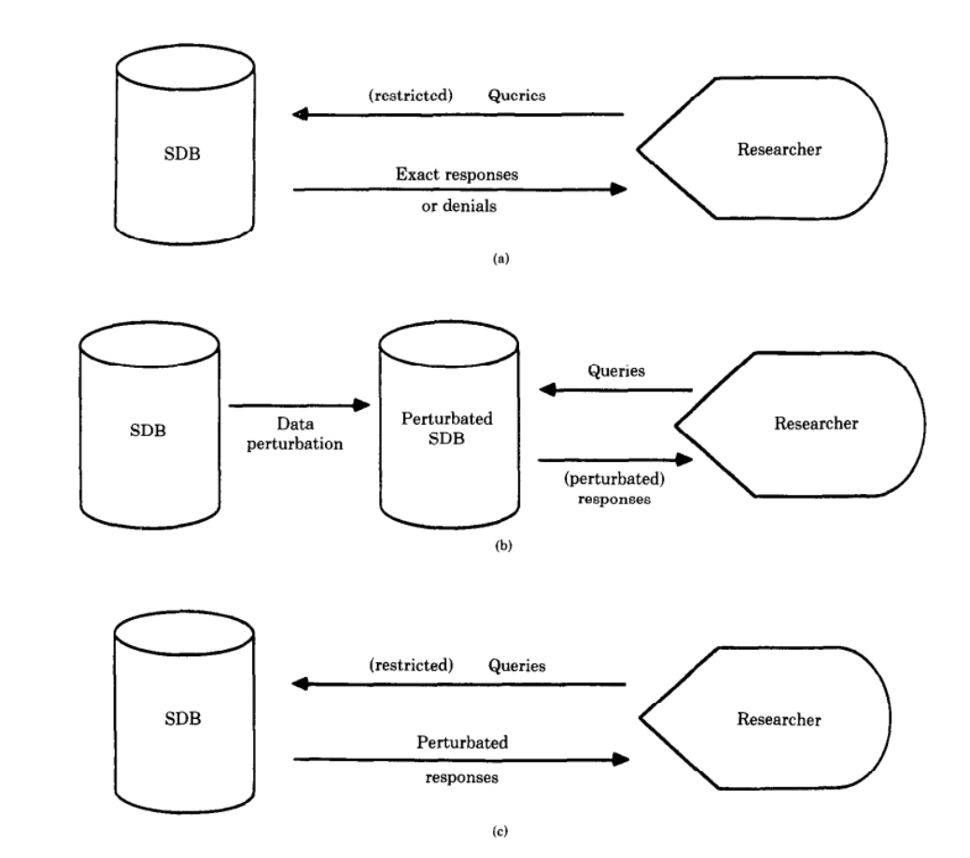
\includegraphics[width=1\linewidth]{assets/text.png}
\caption{Схемы безопасности СБД}
\label{fig:SDB_secure}
\end{figure}

\subsection{Критерии безопасности статистических баз данных}

Критерии безопасности включают оценку вероятности раскрытия записей в СБД, оценку консистентности данных при использовании методов возмущения данных и оценку зависимости между возмущением и конкретными записями. Также учитываются затраты, связанные с выполнением запросов, и назначается конкретная цена каждому запросу. Пользователям предоставляется начальная сумма, которую они могут использовать для запросов, чтобы предотвратить выведение данных.
\\

Когда речь идет о критериях безопасности, необходимо отметить, что полной гарантии безопасности в статистических базах данных (СБД) достичь невозможно. Вместо этого проводится оценка важности деанонимизированных данных и статистической точности, учитывая предпринятые меры по защите данных.
\\

Критерий безопасности "Security" оценивает вероятность раскрытия (включая частичное раскрытие) записи в СБД. Для каждого разрешенного агрегирующего запроса проводится оценка критерия безопасности. Основываясь на количестве информации в базе данных, можно определить, сколько запросов требуется для деанонимизации данных. На основе этой оценки определяется минимальный размер выборки для таких запросов.
\\

Критерий безопасности "Consistency" оценивает консистентность данных для методов возмущения данных. Оценивается степень возмущения данных путем создания агрегирующего запроса и измерения его изменений после внесения возмущений. 
\\

Критерий безопасности "Robustness" оценивает зависимость между возмущением и конкретными записями. Желательно, чтобы возмущение не зависело от данных, однако необходимо сохранить статистические свойства данных.
\\

Критерий безопасности "Costs" определяет конкретную стоимость каждого запроса. Пользователю предоставляется начальная сумма, которую он может использовать для запросов, чтобы предотвратить вывод данных. Этот критерий скорее представляет собой метод управления, а не непосредственный критерий безопасности.
\\

Таким образом, применение критериев безопасности в СБД позволяет оценивать уровень безопасности, учитывая важность данных, статистическую точность, консистентность, робастность и стоимость запросов.
\\

Исходя из вышеизложенных глав, можем убедиться, что безопасность статистических баз данных является сложной задачей, но существуют различные подходы и методы для обеспечения безопасности данных. Каждый подход имеет свои преимущества и недостатки, и выбор методов безопасности должен основываться на анализе конкретных требований и контекста использования СБД. Оценка важности данных, статистической точности и затрат помогает принять решение о применении конкретных методов обеспечения безопасности.



\section{Распознавание вторжений в БД}



\subsection{Основные понятия}

\textbf{Вторжение в БД} -- незаконное или несанкционированное проникновение в базу данных с целью получения несанкционированного доступа к конфиденциальной информации или изменения данных.

\textbf{Обнаружение вторжений} (применительно к БД) -- процесс выявления действий,
которые способны нарушить конфиденциальность, целостность и доступность информации,
хранимой в базе данных (БД).

\textbf{Система обнаружения вторжений} (СОВ) [согласно ФСТЭК [\cite{IDSFSTEK}]] -- программное или
программно-техническое средство, реализующие функции автоматизированного обнаружения
(блокирования) действий в информационной системе, направленных на преднамеренный доступ
к информации, специальные воздействия на информацию (носители информации) в целях ее
добывания, уничтожения, искажения и блокирования доступа к ней.

Применение систем обнаружения вторжения относится к реактивным мерам (то есть к таким
мерам, которые используются уже после того, как произошел инцидент) для противодействия
активности злоумышленника в тех случаях, когда злоумышленник преодолел все проактивные
меры. Поэтому обычно системы обнаружения вторжений являются \textit{вторичным фактором
защиты в общей системе защиты} и предназначены для обнаружения и регистрации уже
произошедних событий, а также оповещение персонала при срабатывании определенных правил.

Если классифицировать методы обнаружения вторжения, используемые в системах обнаружения
вторжений (СОВ), то можно выделить три типа (согласно классификации, предложенной
Стефаном Аксельсоном [\cite{IDSClassification}]):
\begin{itemize}
	\item синтаксические методы (или методы поиска злоупотреблений, англ. misuse detection).
		К таким методам обычно относятся методы, которые основываются на обнаружения
		вторжений путём сравнения SQL-запросов с шаблонами недопустимых синтаксических
		конструкций.

	\item методы обнаружения аномалий (англ. anomaly detection).
		Такие методы, наоборот, в отличие от первого типа, подрузамевают создание шаблонов
		нормального поведения пользователя и последующее сравнение этих шаблонов с действиями,
		выполняемыми пользователями во время работы с БД.

	\item смешанные методы, представляющие собой композицию первых двух
\end{itemize}



\subsection{Системы распознавания вторжений}

Системы обнаружения вторжения (англ. Intrusion Detection System, IDS) и системы
предотвращения вторжений (англ. Intrusion Preventation System, IPS) обычно рассматриваются
вместе, причем часто под термином система предотвращение вторжений подрузамевается
расширение систем обнаружения вторжений, так как IPS системы также должны обладать
возможностью обнаружения вторжений. Иначе говоря, IPS системы являются активными IDS системами.

В IDS системах, система также ответственна за реализацию ответных мер на нарушения:
блокировка соединения, настройки межсетевого экрана и прочее. Таким образом,

\textbf{Система обнаружения и предотвращения вторжений (IPS/IDS)} (применительно к БД) -- это
программное или программно-техническое средство, предназначенное для выявления фактов
неавторизованного доступа и предотвращания попыток несанкционированного доступа к БД.

Обычно архитектура СОВ включает:
\begin{itemize}
	\item сенсорную подсистему, предназначенную для сбора событий, связанных с безопасностью защищаемой системы
	
	\item подсистему анализа, предназначенную для выявления атак и подозрительных действий на основе данных сенсоров
	
	\item хранилище, обеспечивающее накопление первичных событий и результатов анализа
	
	\item консоль управления, позволяющая конфигурировать СОВ, наблюдать за состоянием защищаемой системы и СОВ, просматривать выявленные подсистемой анализа инциденты
\end{itemize}



\subsubsection{Типы моделей систем распознавания вторжений (ID-систем)}

Существует множество способов классификации СОВ, которые не являются однозначными или
обязательными. Следует рассмотреть наиболее известные и используемые классификации,
которые характеризуют систему по:
\begin{itemize}
	\item \textbf{По способу мониторинга}

	\item \textbf{По способу анализа}

	\item \textbf{По скорости реакции}

	\item \textbf{По классу защиты}
\end{itemize}


\paragraph*{По способу мониторинга.}

\begin{itemize}
	\item \textbf{Сетевая СОВ (англ. Network-based IDS, NIDS)} -- система,
	которая занимается проверкой сетевого трафика с концентратора или коммутатора и
	анализируя сетевые пакеты.

	\item \textbf{Узловая СОВ (англ. Host-based IDS, HIDS)} -- система,
	отслеживающая вторжения, используя анализ системных вызовов, логов приложений,
	модификаций файлов (исполняемых, файлов паролей, системных баз данных), состояния
	хоста и прочих источников.
	
	\item \textbf{Основанная на протоколе СОВ (англ. Protocol-based IDS, PIDS)} -- система, которая отслеживает и анализирует коммуникационные протоколы со связанными системами или пользователями. Для веб-сервера подобная СОВ обычно ведет наблюдение за HTTP и HTTPS протоколами. При использовании HTTPS СОВ должна располагаться на таком интерфейсе, чтобы просматривать HTTPS пакеты ещё до их шифрования и отправки в сеть.

	\item \textbf{Основанная на прикладных протоколах СОВ (англ. Application-based IDS, APIDS)} --
	система, в которой ведется наблюдение за специализированными прикладными протоколами
	и анализ соответствующих данных. Например, на веб-сервере с SQL базой данных СОВ будет
	отслеживать содержимое SQL команд, передаваемых на сервер.

	\item \textbf{Гибридная СОВ} -- система, которая является композицией нескольких видов
	систем обнаружения вторжений.
\end{itemize}


\paragraph*{По способу анализа.}

Данная классификация строится по методу анализа событий,
полученных из источника информации, и методу принятия решения, что происходит
проникновение. Способами анализа являются методы \textbf{основанные на сигнатурах} и
\textbf{основанные на аномалиях}.

\textbf{СОВ на основе сигнатур} - это обнаружение атак путем поиска определенных шаблонов, таких как последовательности байтов в сетевом трафике или известные последовательности инструкций, используемые вредоносным ПО. Эта терминология берет начало в антивирусном программном обеспечении, которое называет эти обнаруженные шаблоны сигнатурами. Хотя IDS на основе сигнатур могут легко обнаружить известные атаки, им сложно обнаружить новые атаки, для которых не существует шаблонов [\cite{NetSecChristos}].

\textbf{СОВ на основе аномалий} были созданы в первую очередь для обнаружения неизвестных атак, отчасти из-за быстрого развития вредоносного ПО. Основной подход заключается в использовании машинного обучения для создания модели достоверной активности, а затем сравнения нового поведения с этой моделью. Поскольку эти модели могут быть обучены в зависимости от приложений и конфигурации оборудования, метод машинного обучения обладает лучшими обобщенными свойствами по сравнению с традиционными IDS на основе сигнатур. Хотя этот подход позволяет обнаруживать ранее неизвестные атаки, он может страдать от ложных срабатываний: ранее неизвестная легитимная активность может быть классифицирована как вредоносная. Большинство существующих IDS страдают от того, что процесс обнаружения занимает много времени, что снижает производительность IDS. Эффективный алгоритм выбора признаков делает процесс классификации, используемый при обнаружении, более надежным[\cite{Rowayda}].

\paragraph*{По скорости реакции.}

Определяют два типа СОВ по времени между получением информации из источника и ее
анализом и принятием решения. В зависимости от задержки во времени, СОВ разделятся на:
\begin{itemize}
	\item \textbf{с пакетным режимом (англ. interval-based)}. В таких системах реакция
	происходит через определенные интервалы времени, а информационный поток от точек
	мониторинга до инструментов анализа не является непрерывным.

	\item \textbf{непрерывные (англ. real-time)}. В таких системах обрабатывается
	непрерывный поток информации от источников. При этом таких тип является преобладающей
	типом в сетевых СОВ, которые получают информацию из потока сетевого трафика.
\end{itemize}


\paragraph*{По классу защиты.}

Для каждой сертифицированной в России СОВ присваивается некоторый класс защиты
согласно классификации ФСТЭК и выполненным требованиям для определенного профиля защиты (ПЗ).
Всего существует 6 классов, где самый низкий класс - шестой, а самый высокий - первый.

Согласно ФСТЭК СОВ разделяются на [\cite{IDSFSTEK}]:
\begin{itemize}
	\item \textbf{СОВ с 6 классом защиты}: применяются в информационных системах
	персональных данных 3 и 4 классов.

	\item \textbf{СОВ с 5 классом защиты}: применяются в информационных системах
	персональных данных 2 класса.

	\item \textbf{СОВ с 4 классом защиты}: применяются в государственных информационных
	системах, в которых обрабатывается информация ограниченного доступа, не содержащая
	сведения, составляющие государственную тайну, в информационных системах персональных
	данных 1 класса, а также в информационных системах общего пользования II класса.

	\item \textbf{СОВ с 3, 2 или 1 классом защиты}: применяются в информационных системах,
	в которых обрабатывается информация, содержащая сведения, составляющие государственную
	тайну.
\end{itemize}



\subsubsection{Общая структура ID-систем}


\paragraph*{Архитектура СОВ.} Основнымы архитектурными компонентами СОВ являются:

\begin{enumerate}
	\item \textbf{Host} -- система, на которой выполняется ПО СОВ.

	\item \textbf{Target} -- система, за которой наблюдает СОВ.
\end{enumerate}

Первоначально многие СОВ выполнялись на тех же системах, которые они защищали.
Основная причина этого была в том, что большинство систем было mainframe, и стоимость
выполнения СОВ на отдельном компьютере была очень большой. Это создавало проблему с
точки зрения безопасности, так как любой атакующий, который успешно атаковал целевую
систему, мог в качестве одной из компонент атаки просто запретить функционирование СОВ.

Но с появлением рабочих станций и персональных компьютеров в большинстве архитектур
СОВ предполагается выполнение СОВ на отдельной системе, тем самым разделяя системы
Host и Target. Это улучшает безопасность функционирования СОВ, так как в этом случае
проще спрятать существование СОВ от атакующих.


\paragraph*{Компоненты современных СОВ:}

\begin{itemize}
	\item сенсор, который отслеживает события в сети или системе;

	\item анализатор событий, обнаруженных сенсорами;

	\item компонента принятия решения.
\end{itemize}


\paragraph*{Способы управления СОВ:}

\begin{itemize}
	\item \textbf{Централизованное управление}. При централизованных стратегиях управления
	весь мониторинг, обнаружение и отчетность управляются непосредственно с единого "поста".
	В этом случае существует единственная консоль СОВ, которая связана со всеми сенсорами,
	расположенными в сети.

	\item \textbf{Частично распределенное управление}. Мониторинг и определение управляются
	с локально управляемого узла, с иерархической отчетностью в одно или более центральных
	расположений.

	\item \textbf{Полностью распределенное управление}. Мониторинг и определение выполняются
	с использованием подхода, основанного на агентах, когда решения об ответе делаются в
	точке анализа.
\end{itemize}

При этом в сети должны поддерживаться следующие связи:

\begin{itemize}
	\item связи для передачи отчетов СОВ. Эти связи создаются между сенсорами как сетевого
	мониторинга, так и мониторинга хоста, и центральной консолью СОВ;

	\item связи для мониторинга хостов и сетей;

	\item связи для выполнения ответов СОВ.
\end{itemize}

\subsubsection{Определение сигнатур (злоупотреблений)}

Детекторы злоупотреблений анализируют деятельность системы, анализируя событие или множество событий на соответствие заранее определенному образцу, который описывает известную атаку. Соответствие образца известной атаке называется сигнатурой, определение злоупотребления иногда называют ``сигнатурным определением''. Наиболее общая форма определения злоупотреблений, используемая в коммерческих продуктах, специфицирует каждый образец событий, соответствующий атаке, как отдельную сигнатуру. \autocite{IntrusionDetectionSystemsMsu}

Тем не менее существует несколько более сложных подходов для выполнения определения злоупотреблений (называемых state-based технологиями анализа), которые могут использовать единственную сигнатуру для определения группы атак.


Обнаружение злоупотреблений позволяет идентифицировать несанкционированные действия, если имеется их точное представление в виде шаблонов атак. Здесь под шаблоном атаки понимается некоторая совокупность явно описывающих конкретную атаку действий (правил сопоставления, вывода), применяя которые к признакам и полям идентифицируемого объекта можно получить однозначный ответ о его принадлежности к этой атаке. \autocite{IDSBranitsky}

\paragraph*{Преимущества определения злоупотреблений:}

\begin{itemize}
	\item Детекторы злоупотреблений являются очень эффективными для определения атак и не создают при этом огромного числа ложных сообщений.

	\item Детекторы злоупотреблений могут быстро и надежно диагностировать использование конкретного инструментального средства или технологии атаки. Это может помочь администратору скорректировать меры обеспечения безопасности.
	
	\item Детекторы злоупотреблений позволяют администраторам, независимо от уровня их квалификации в области безопасности, начать процедуры обработки инцидента.
\end{itemize}


\paragraph*{Недостатки определения злоупотреблений:}

\begin{itemize}
	\item Детекторы злоупотреблений могут определить только те атаки, о которых они знают, следовательно, надо постоянно обновлять их базы данных для получения сигнатур новых атак.

	\item Многие детекторы злоупотреблений разработаны таким образом, что могут использовать только строго определенные сигнатуры, а это не допускает определения вариантов общих атак.
\end{itemize}

Подытоживая сказанное, отметим, что методы обнаружения злоупотреблений являются эффективным инструментом для выявления известных типов атак, но их применимость по отношению к новым атакам,
а также к модификациям известных атак является безрезультативной.


\subsubsection{Определение аномалий и шаблоны классов пользователей}

Рассматривать шаблоны классов пользователей имеет смысл только в контексте СОВ,
применяющих методы обнаружения аномалий, так как именно они строят и используют
такие шаблоны поведения пользователей. Таким образом, детекторы аномалий определяют
необычное поведение на хосте или в сети. Они предполагают, что атаки отличаются от
некоторой нормальной деятельности и могут, следовательно, быть определены системой,
которая умеет отслеживать эти отличия. Детекторы аномалий создают профили, представляющие
собой нормальное поведение пользователей, хостов или сетевых соединений. Эти профили
создаются, исходя из данных истории, собранных в период нормального функционирования.
Затем детекторы собирают данные о событиях и используют различные метрики для определения
того, что анализируемая деятельность отклоняется от нормальной.

Метрики и технологии, используемые при определении аномалий, включают:

\begin{itemize}
	\item определение допустимого порога. В этом случае основные атрибуты поведения
	пользователя и системы выражаются в количественных терминах. Для каждого атрибута
	определяется некоторый уровень, который устанавливается как допустимый. Такие атрибуты
	поведения могут определять число файлов, доступных пользователю в данный период времени,
	число неудачных попыток входа в систему, количество времени ЦП, используемое процессом и
	т.п. Данный уровень может быть статическим или эвристическим — например, может определяться
	изменением анализируемых значений.

	\item статистические метрики: параметрические, при которых предполагается, что распределение
	атрибутов профиля соответствует конкретному образцу, и непараметрические, при которых
	распределение атрибутов профиля является "обучаемым" исходя из набора значений истории,
	которые наблюдались за определенный период времени.

	\item метрики, основанные на правилах, которые аналогичны непараметрическим статистическим
	метрикам в том, что наблюдаемые данные определяют допустимые используемые образцы, но
	отличаются от них в том, что эти образцы специфицированы как правила, а не как численные
	характеристики.

	\item другие метрики, включая нейросети, генетические алгоритмы и модели иммунных систем.
\end{itemize}


\paragraph*{Преимущества определения аномалий:}

\begin{itemize}
	\item IDS, основанные на определении аномалий, обнаруживают неожиданное поведение и,
	таким образом, имеют возможность определить симптомы атак без знания конкретных деталей атаки.

	\item Детекторы аномалий могут создавать информацию, которая в дальнейшем будет
	использоваться для определения сигнатур для детекторов злоупотреблений.
\end{itemize}


\paragraph*{Недостатки определения аномалий:}

\begin{itemize}
	\item Подходы определения аномалий обычно создают большое количество ложных сигналов
	при непредсказуемом поведении пользователей и непредсказуемой сетевой активности.

	\item Подходы определения аномалий часто требуют некоторого этапа обучения системы,
	во время которого определяются характеристики нормального поведения.
\end{itemize}



\subsubsection{Модели известных атак}

\textbf{SQL инъекция} -- это форма атаки на веб-приложение, при которой злоумышленник внедряет вредоносный SQL код в строку запроса к базе данных. Целью такой атаки является получение доступа к конфиденциальным данным, изменение информации в базе данных или даже удаление всех данных из базы. SQL инъекции возникают из-за недостаточной защиты от них в коде приложения, что позволяет злоумышленнику использовать уязвимости для выполнения опасных операций.

Все типы инъекций делятся на три основных:
\begin{itemize}
	\item Внутриполосные SQL -- проводятся внутриполосно, являются наиболее распространенными и легко эксплуатируемыми. При внутриполосной SQL-инъекции злоумышленник может и запустить атаку, и собрать результаты по одному и тому же каналу связи.
	
	\item Инференциальная SQL -- инъекция также известна как слепая. В отличие от внутриполосной SQL-инъекции, инференциальная SQL-инъекция может занять больше времени у злоумышленников. В  данном типе атаки злоумышленник не может напрямую увидеть ответы на внедренные запросы, поскольку данные не передаются между веб-приложениями. Вместо этого уязвимости такого рода эксплуатируются путем наблюдения за поведением приложения с целью перебора базы данных. 
	
	\item Внеполосные SQL -- инъекции,которые встречаются нечасто, так как зависят от возможностей сервера баз данных веб-приложения. Если злоумышленник не может провести атаку и получить результаты по одному и тому же каналу, атака называется внеполосной SQL-инъекцией. При внеполосной атаке злоумышленник манипулирует целевым приложением, чтобы отправить данные на удаленную конечную точку, находящуюся под его контролем, а не получить от нее ответ. 	Если ваш сервер запускает DNS- или HTTP-запросы, то вы можете осуществить внеполосную SQL-инъекцию. 
\end{itemize}

Далее будут рассмотрены основные типы SQL-инъекций \autocite{proglib},\autocite{SqlInjection} на простом примере критически уязвимой страницы
\begin{figure}[h]
    \centering
    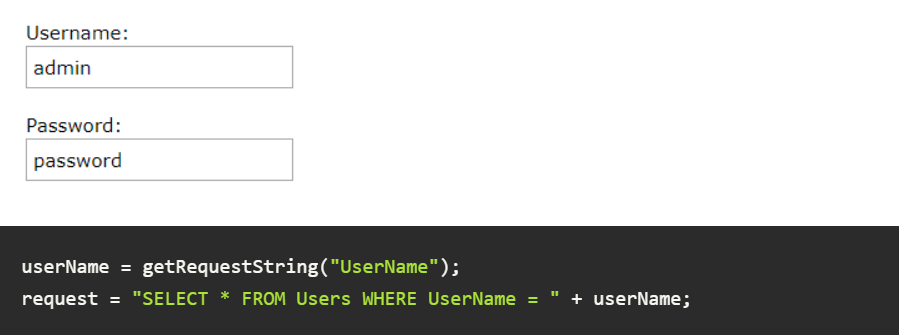
\includegraphics[width=0.8\textwidth]{assets/sql_ijection_example.png}
    \caption{Пример уязвимой страницы}
    \label{fig:mesh}
\end{figure}

\begin{itemize}
    \item \textbf{Атаки комментированием}\\
    Использование однострочных комментариев позволяет игнорировать часть запроса, идущую после вашей инъекции. Например, ввод в уязвимое поле Username запроса admin'-- позволит зайти на ресурс под администратором, потому что поверка пароля будет закомментирована.\\
    \begin{grayquote}
        SELECT * FROM members WHERE username = 'admin'--' AND password = 'password'
    \end{grayquote}

    Многострочные комментарии могут справится с проверкой или определить тип базы данных.
    Например, подобные запросы обойдут примитивный текстовый анализ:\\
    \begin{grayquote}
        DROP/*some comment*/sampletable\\
        DR/**/OP/*random comment to cheat*/sampletable
    \end{grayquote}

    \item \textbf{Манипуляции со строками}\\
    При помощи конкатенации строк можно обходить фильтр кавычек.\\
    \begin{grayquote}
        SELECT CONCAT(login, password) FROM members
    \end{grayquote}

    Можно представлять строки в шеснадцатиричном виде, с помощью функции HEX() или вводить их посимвольно.
    \begin{grayquote}
        //0x633A5C626F6F742E696E69 == c:\textbackslash boot.ini\\
        SELECT CONCAT('0x','633A5C626F6F742E696E69'))\\
        SELECT CONCAT(CHAR(75),CHAR(76),CHAR(77))
    \end{grayquote}

    \item \textbf{Обход аутентификации}\\
    При помощи OR и сравнения констант можно обойти форму аутентификации. Существуют даже словари, содержащие основные запросы для обхода уязвимой формы

    Примеры запросов:\\
    \begin{grayquote}
        ' or 1=1\\
        ' or 1=1--\\
        ' or 1=1\#\\
        admin' --\\
        admin' or '1'='1
    \end{grayquote}

    \item \textbf{Union injection}\\
    При помощи UNION комбинировать данные из разных таблиц в одну. Это одна из самых популярных и опасных классических инъекций.

    Допустим, на сайте есть список товаров с уязвимой строкой поиска. Тогда, подобрав правильное количество колонок и определив их название, через UNION можно вывести практически любые данные
    \begin{grayquote}
        SELECT name, price FROM products UNION ALL SELECT name, pass FROM members\\
        \#Такой запрос позволит получить данные о таблицах и найти таблицу пользователей\\
        UNION(SELECT TABLE\_NAME,

        TABLE\_SCHEMA FROM information\_schema.tables)
    \end{grayquote}

    \item \textbf{Расщепление SQL-запроса}\\
    В некоторых СУБД можно использовать простой знак ';' для последовательного вызова вредоносных запросов.
    
    Например, если в параметры скрипта
    \begin{grayquote}
    	\$id = \$\_REQUEST['id'];\\
    	\$res = mysql\_query("SELECT * FROM news WHERE id\_news = \$id");  
    \end{grayquote}
    злоумышленником передается конструкция, содержащая точку с запятой, например 12;INSERT INTO admin (username, password) VALUES ('HaCkEr', 'foo'); то в одном запросе будут выполнены 2 команды    	
    \begin{grayquote}
		SELECT * FROM news WHERE id\_news = 12;\\
   	 	INSERT INTO admin (username, password) VALUES ('HaCkEr', 'foo');
    \end{grayquote}
    и в таблицу admin будет несанкционированно добавлена запись HaCkEr.
    
    Также можно, к примеру, удалить таблицу или выключить SQL сервер.
    
    \begin{grayquote}
        \#Удаление таблицы\\
        SELECT * FROM products WHERE productName = ""; DROP users--\\
        \#Выключение SQL Server\\
        SELECT * FROM products WHERE productName = ""; shutdown –
    \end{grayquote}


    \item \textbf{Error-based injection}\\
    Инъекции, основанные на том, что злоумышленник может видеть вывод ошибки. Уязвимость устраняется просто отключением этого вывода

    Последовательное выполнение следующих запросов может помочь определить в тексте ошибки названия столбцов:\\
    \begin{grayquote}
        ' HAVING 1=1 --\\
        ' GROUP BY table.columnfromerror1 HAVING 1=1 --\\
        ' GROUP BY table.columnfromerror1, columnfromerror2 HAVING 1=1 --\\
        .....\\
        ' GROUP BY table.columnfromerror1, columnfromerror2, columnfromerror(n) HAVING 1=1 --\\
        Если ошибки перестали появляться, значит столбцы закончились
    \end{grayquote}

    \item \textbf{Boolean-based blind injection}\\
    Если атакующий все же может получить информацию о наличии или отсутствии ошибки из HTTP-статуса, в сервисе имеется уязвимость к обычной слепой атаке. Рассмотрим запрос, который позволит нам при помощи алгоритма бинарного поиска посимвольно определить название первой таблицы и в дальнейшем всех данных

    \begin{grayquote}
        TRUE : SELECT ID, Username, Email FROM [User]WHERE ID = 1 AND \\
        ISNULL(ASCII(SUBSTRING((SELECT TOP 1 name FROM sysObjects WHERE xtYpe=0x55 AND\\
        name NOT IN(SELECT TOP 0 name FROM sysObjects WHERE xtYpe=0x55)),1,1)),0)>78--\\
        \#Этот запрос говорит нам, что ASCII-значение первого символа больше 78 \\
        \#дальнейший перебор определит точное значение
    \end{grayquote}

    \item \textbf{Time-based blind injection}\\
    Если атакующий не наблюдает никаких отличий в ответах сервера, можно попробовать SLEEP или WAIT FOR DELAY

    \begin{grayquote}
        SELECT * FROM products WHERE id=1; WAIT FOR DELAY '00:00:15'
    \end{grayquote}
    Конечно, реальные примеры будут выглядеть примерно как boolean-based, только true и false атакующий будет отличать по времени отклика
    
        \item \textbf{Внедрение в строковые параметры}\\
   Предположим, серверное ПО, получив запрос на поиск данных в новостях параметром search\_text, использует его в следующем SQL-запросе (здесь параметры экранируются кавычками):\\
    \begin{grayquote}
    	\$search\_text = \$\_REQUEST['search\_text'];\\
    	\$res = mysqli\_query("SELECT id\_news, news\_date, news\_caption, news\_text, news\_id\_author\\
    	FROM news WHERE news\_caption LIKE('\%\$search\_text\%')");
    \end{grayquote}
    
    Сделав запрос вида http://example.org/script.php?search\_text=Test мы получим выполнение следующего SQL-запроса:\\
    \begin{grayquote}
    	SELECT id\_news, news\_date, news\_caption, news\_text, news\_id\_author FROM news 
    	WHERE news\_caption LIKE('\%Test\%')
    \end{grayquote}
    
        Но, внедрив в параметр search\_text символ кавычки (который используется в запросе), мы можем кардинально изменить поведение SQL-запроса. Например, передав в качестве параметра search\_text значение ')+and+(news\_id\_author='1, мы вызовем к выполнению запрос:\\
    \begin{grayquote}
    	SELECT id\_news, news\_date, news\_caption, news\_text, news\_id\_author FROM news 
    	WHERE news\_caption LIKE('\%') and (news\_id\_author='1\%')
    \end{grayquote}
    
    
\end{itemize}



\subsection{Экспертные ID-системы}

Название "экспертная система" происходит из термина "экспертная система, базирующаяся на знаниях". Экспертная система – это система, которая использует человеческие знания, встраиваемые в компьютер, для решения задач, которые обычно требуют человеческой экспертизы. Хорошо разработанные системы имитируют процесс рассуждения экспертов, используя это для решения специфических задач.

Технологию построения экспертных систем часто называют инженерией имплекационных правил. Как правило,
этот процесс требует специфической формы взаимодействия создателя имплекационных правил и одного
или нескольких экспертов в некоторой предметной области. Инженер имплекационных правил "встраивает"
процедуры, стратегии, эмпирические правила в экспертную систему. В результате появляется
компьютерная программа, которая решает задачи во многом так же, как эксперты -- люди.
\autocite{IDSystem}

Главное преимущество использования продукционных систем заключается в возможности разделения причин и
решений возникающих проблем.

В экспертных системах могут использоваться импликационные правила (\textbf{Если} \textit{условие} то
\textbf{действие}).

Например:
\begin{itemize}
	\item ЕСЛИ с одного узла за время T поступает N пакетов, ТО записать в лог факт:
	происходит DoS атака (факт А)

	\item Если наблюдается более чем N фактов А, ТО записать в лог факт: происходит DDoS атака
\end{itemize}

Основные проблемы, которые обычно возникают при их практическом применении:
\begin{itemize}
    \item Недостаточная эффективность при работе с большими объемами данных.
    \item Трудно учесть зависимую природу данных параметров оценки.
\end{itemize}

При использовании экспертных систем для обнаружения вторжений можно установить символическое
проявление вторжения при помощи имеющихся данных.

\textbf{Трудности:}
\begin{itemize}
    \item Отсутствие встроенной или естественной обработки порядка последовательностей в анализируемых
    данных. База фактов, соответствующая левой части «продукции», используется для определения правой
    части. В левой части продукционного правила все элементы объединяются при помощи связи «и».
    \item Встроенная экспертиза хороша только в том случае, если моделируемые навыки администратора
    безопасности не противоречивы. Это практическое рассуждение, возможно, касается
    недостаточной централизованности усилий экспертов безопасности в направлении создания
    исчерпывающих множеств правил. Обнаруживаются только известные уязвимости.
    \item Существуют определенный программный инжиниринг, связанный с установкой (поддержанием) баз знаний.
    При добавлении или удалении какого-либо из правил должно изменяться остальное множество правил.
    \item Обнаруживаются только известные уязвимости.
    \item Объединение различных измерений вторжений и создание связанной картины вторжения приводит к
    тому, что частные причины становятся неопределенными. Ограничения продукционных систем, в
    которых используется неопределенная причина, довольно хорошо известны.
\end{itemize}
\autocite{BeynonDavies}



\subsubsection{Метрики}

\begin{itemize}
	\item \textbf{Показатель активности} -- величина, при превышении которой активность
	подсистемы оценивается как быстро прогрессирующая. В общем случае используется для
	обнаружения аномалий, связанных с резким ускорением в работе. Пример: среднее число
	записей аудита, обрабатываемых для элемента защищаемой системы в единицу времени.

	\item \textbf{Распределение активности в записях аудита} -- распределение во всех типах
	активности в актуальных записях аудита. Здесь под активностью понимается любое действие
	в системе, например, доступ к файлам, операции ввода-вывода.

	\item \textbf{Измерение категорий} -- распределение определенной активности в
	категории \footnotemark. Например, относительная частота количества регистраций в
	системе (логинов) из каждого физического места нахождения. Предпочтения в использовании
	программного обеспечения системы (почтовые службы, компиляторы, командные интерпретаторы,
	редакторы и т.д.)

	\item \textbf{Порядковые измерения} -- используется для оценки активности, поступающей
	в виде цифровых значений. Например, количество операция ввода-вывода, инициируемых каждым
	пользователем. Порядковые изменения вычисляют общую числовую статистику значений определенной
	активности, в то время как измерение категорий подсчитывает количество активностей.
\end{itemize}
\autocite{BeynonDavies}
\footnotetext{Здесь под \textit{категорией} понимается группа подсистем, объединенных по
некоему общему принципу}



\subsubsection{Статистические модели}

При обнаружении аномалий с использованием профайла в основном применяют статистические
методы оценки. Процесс обнаружения происходит следующим образом: текущие значения измерений
профайла сравнивают с сохраненными значениями. Результат сравнения - показатель аномальности
в измерении. Общий показатель аномальности в простейшем случае может вычисляться при помощи
некоторой общей функции от значений показателя аномалии в каждом измерении профайла.

Например, пусть $M_1, M_2, \dots, M_n$ -- измерения профайла, а $S_1, S_2, \dots, S_n$ --
соответственно представляют собой значения аномалии каждого из измерений. Чем больше
число $S_i$, тем больше аномалии в $i$-ом показателе. Объединяющая функция может быть
взвешенной суммой их квадратов:

\begin{equation}
	a_1s_1^2 + a_2s_2^2 + \dots + a_ns_n^2 > 0,
\end{equation}

где $a_i$ -- отражает относительный вес метрики $M_i$.

Параметры $M_1, M_2, \dots, M_n$ могут быть зависимыми друг от друга. В таком случае,
объединяющая функция будет более сложной.\autocite{IDSystem}

\textbf{Основное преимущество} заключается в том, что применяются хорошо известные статистические методы.

\textbf{Недостатки:}
\begin{itemize}
	\item Нечувствительность к последовательности возникновения событий.
	То есть статистическое обнаружение может упустить вторжение,
	которое проявляется в виде последовательности сходных событий.

	\item Система может быть последовательно обучена таким образом, что аномальное поведение
	будет считаться нормальным. Злоумышленники, которые знают, что за ними наблюдают
	при помощи таких систем, могут обучить их для использования в своих целях. Именно поэтому в
	большинстве существующих схем обнаружения вторжения используется комбинация подсистем
	обнаружения аномалий и злоупотреблений.

	\item Трудно определить порог, выше которого аномалии можно рассматривать как вторжение.
	Занижение порога приводит к ложному срабатыванию (false positive), а завышение – к пропуску вторжений (false negative).

	\item Существуют ограничения к типам поведения, которые могут быть смоделированы,
	используя чистые статистические методы. Применение статистических технологий для
	обнаружения аномалий требует предположения, что данные поступают от квазистатического процесса.
\end{itemize}
\autocite{IntrusionDetection}


\subsubsection{Профили}

Одним из способов формирования "образа" нормального поведения системы состоит в
накоплении измерений значения параметров оценки в специальной структуре данных.
Эта структура данных называется \textit{профайлом}.\autocite{IDSystem}

Основные требования, предъявляемые к структуре профайла:
\begin{itemize}
	\item Минимальный конечный размер

	\item Быстрое выполнение операции обновления
\end{itemize}



\subsubsection{Нейронные сети для представления профиля}
Другой способов представления "образа" нормального поведения системы – обучение нейронной
сети значениями параметров оценки.

Обучение нейронной сети осуществляется последовательностью информационных единиц (далее команд),
каждая из которых может находиться на более абстрактном уровне по сравнению с используемыми
параметрами оценки. Входные данные сети состоят из текущих команд и прошлых \textbf{W} команд, которые
обрабатываются нейронной сетью с целью предсказания последующих команд; \textbf{W} также называют размером
окна. После того как нейронная сеть обучена множеством последовательных команд защищаемой системы или
одной из ее подсистем, сеть представляет собой «образ» нормального поведения. Процесс обнаружения
аномалий представляет собой определение показателя неправильно предсказанных команд,
то есть фактически обнаруживается отличие в поведение объекта. На уровне рецептора стрелки
показывают входные данные последних \textbf{W} команд, выполненных пользователем. Входной параметр задает
несколько значений или уровней, каждый из которых уникально определяет команду. Выходной реагирующий
слой состоит из одного многоуровневого, который предсказывает следующую возможную команду пользователя.
\autocite{BeynonDavies}

\begin{figure}[h!]
    \centering
    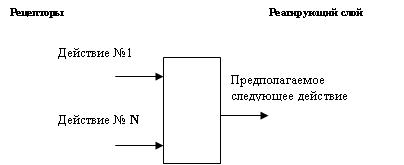
\includegraphics[width=0.8\textwidth]{assets/intrusion/neural_networks.jpg}
\end{figure}

\textbf{Недостатки:}
\begin{itemize}
    \item Топология сети и веса узлов определяются только после огромного числа проб и ошибок.
    \item Размер окна – еще одна величина, которая имеет огромное значение при разработке.
    Если сделать окно маленьким то сеть будет не достаточно производительной, слишком большим
    – будет страдать от неуместных данных.
\end{itemize}

\textbf{Преимущества:}
\begin{itemize}
    \item Успех данного подхода не зависит от природы исходных данных.
    \item Нейронные сети легко справляются с зашумленными данными.
    \item Автоматически учитываются связи между различными измерениями, которые,
    несомненно, влияют на результат оценки.
\end{itemize}
\autocite{BeynonDavies}


\subsubsection{Нейронные сети для представления профиля}
Представление «образа» в данном случае основывается на предположении о том, что текущие значения
параметров оценки можно связать с текущим состоянием системы. После этого функционирование
представляется в виде последовательности событий или состояний.

Были предложены временные правила, которые характеризуют совокупности значений параметров оценки
(далее паттерна) нормальной (не аномальной) работы. Эти правила формируются индуктивно и заменяются
более «хорошими» правилами динамически во время обучения. Под «хорошими правилами» понимаются правила
с большей вероятностью их появления и с большим уровнем уникальности для защищаемой системы.
Для примера рассмотрим следующее правило:

\begin{equation}
	E1 \rightarrow E2\rightarrow E3 \Rightarrow E4 = 0.95, E5 = 0.05
\end{equation}
где Е1\dotsЕ5 - события безопасности.

Это утверждение, основанное на ранее наблюдавшихся данных, говорит о том, что для последовательности
паттернов установилась следующая зависимость: если имеет место \textbf{Е1} и далее \textbf{Е2} и \textbf{Е3},
то после этого вероятность проявления \textbf{Е4} - 0.95 и \textbf{Е5} – 0.05.

Именно множество правил, создаваемых индуктивно во время наблюдения работы пользователя, составляет «образ».
Аномалия регистрируется в том случае, если наблюдаемая последовательность событий соответствует левой
части правила выведенного ранее, а события, которые имели место в системе после этого,
значительно отличаются от тех, которые должны были наступить по правилу.

\textbf{Основной недостаток} данного подхода заключается в том, что неузнаваемые паттерны поведения могут
быть не приняты за аномальные из-за того, что они не соответствуют ни одной из левых частей
всех правил.\autocite{IDSystem}

Данный метод довольно эффективно определяет вторжения, так как принимаются во внимание:
\begin{itemize}
    \item Зависимости между событиями.
    \item Последовательность появления событий.
\end{itemize}

\textbf{Достоинства метода:}
\begin{itemize}
    \item Лучшая обработка пользователей с большим колебанием поведения, но с четкой
    последовательностью паттернов.
    \item Возможность обратить внимание на некоторые важные события безопасности, а не на всю сессию,
    которая помечена как подозрительная.
    \item Лучшая чувствительность к обнаружению нарушений: правила содержат в себе семантику процессов, что позволяет гораздо проще заметить злоумышленников, которые пытаются обучить систему в своих целях.
\end{itemize}
\autocite{IntrusionDetection}

\subsubsection{Примеры ID-систем}


\paragraph*{GreenSQL} (APIDS система) -- межсетевой экран, функционирующий как
прокси-сервер между веб-приложением и SQL сервером. То есть приложение устанавливает
соединения к БД не напрямую, а через сервер GreenSQL. GreenSQL анализирует SQL запросы
на предмет аномальных запросов, и в случае нормального запроса (то есть если степень
риска запроса мала) перенаправляет его на внутренний сервер БД.

GreenSQL поддерживает следующие режимы работы:
\begin{itemize}
	\item \textbf{Режим симуляции (англ. Simulation Mode)} -- пассивная система обнаружения
	атак (IDS). Протоколирует SQL запросы, выдает предупреждения на консоль управления.

	\item \textbf{Блокировка подозрительных команд (англ. Blocking Suspicious Commands/Risk Based)} --
	активная СОВ. Атаки не только обнаруживаются, но и блокируются (IPS) в соответствии с
	установленными правилами, указывающими на аномальность запроса.

	\item \textbf{Активная защита от неизвестных запросов (англ. Database Firewall)} --
	блокирование всех неизвестных запросов.

	\item \textbf{Режим обучения (англ. Learning mode)} -- предназначен для прогона и
	настройки правил в <<чистой>> среде, что позволяет сформировать белый список и
	предотвратить в последствии ложные срабатывания анализатора запросов.
\end{itemize}

Особенности GreenSQL:
\begin{itemize}
	\item Поддержка ряда СУБД: Microsoft SQL 2000/2005/2008, MySQL 4.x/5.x, PostgreSQL 7.x/8.x.

	\item Является кросс-платформенной. Среди официально поддерживаемых платформ Microsoft
	Windows Server 2003/2008, Ubuntu, CentOS. Поддерживаются 32-х и 64-х разрядные системы.

	\item GreenSQL находит подозрительные запросы, используя ряд методов:
	\begin{itemize}
		\item Путем определения административных и чувствительных команд SQL.
		Например: SHOW TABLES, CREATE TABLE, ALTER TABLE.

		\item Путем подсчета риска запроса. На это может влиять пустая строка пароля, "or"
		внутри запроса или выражения SQL, которые всегда возвращают истину (1=1).
	\end{itemize}

\end{itemize}


\paragraph*{Snort} (NIDS система) -- свободная сетевая система предотвращения вторжений (IPS)
и обнаружения вторжений (IDS) с открытым исходным кодом, способная выполнять регистрацию
пакетов и в реальном времени осуществлять анализ трафика в IP-сетях.

Snort поддерживает следующие режимы работы:
\begin{itemize}
	\item \textbf{Sniffer mode}. В таком режиме программа только считывает сетевые пакеты и
	выводит их на консоль.

	\item \textbf{Packet Logger Mode}. В режиме логирования пакетов, программа будет
	регистрировать/логировать пакеты на диске.

	\item \textbf{Network Intrusion Detection System Mode}. В режиме обнаружения вторжений
	программа будет отслеживать сетевой трафик и анализировать его в соответствии с набором
	правил, определенным пользователем. Затем программа выполнит определенное действие,
	основанное на том, что было идентифицировано.
\end{itemize}

Особенности Snort:
\begin{itemize}
	\item Возможность написания собственных правил.
	\item Расширение функциональности с помощью подключения дополнительных модулей.
	\item Гибкая система оповещения об атаках: Log-файлы, устройства вывода, БД и прочие.
\end{itemize}


\paragraph*{Suricata} (NIDS система) -- свободная сетевая система предотвращения вторжений
(IPS) и обнаружения вторжений (IDS) с открытым исходным кодом. Основана разработчиками,
которые трудились над IPS версией Snort, поэтому имеет схожий функционал и обладает полной
поддержкой формата правил Snort.

Особенности Suricata:
\begin{itemize}
	\item Многозадачность.

	\item Автоматическое определение протокола.

	\item Высокая производительность, позволяющая обрабатывать трафик до 10Gbit на обычном
	оборудовании.
\end{itemize}


\paragraph*{Sagan} (HIDS система) -- многопоточная, высокопроизводительная система
анализа журналов и мониторинга появления в логах событий, связанных с безопасностью,
и реагирования на эти события в режиме реального времени. Система работает в операционных
системах Unix.

Sagan также относится к категории систем управления инцидентами и событиями информационной
безопасности (англ. Security Information and Log Management, SEIM).

\subsubsection{Недостатки существующих систем обнаружения}

Недостатки современных систем обнаружения можно разделить на две группы – недостатки, связанные со структурой СОВ, и недостатки, относящиеся к реализованным методам обнаружения.

\paragraph*{Недостатки структур СОВ.}

\begin{itemize}
	\item Отсутствие общей методологии построения. Частично это можно объяснить недостаточностью общих соглашений в терминологии, так как СОВ – это достаточно новое направление, основанное Андерсоном (J.P. Anderson) в 1980 г.
	\item Эффективность. Часто методы системы пытаются обнаружить любую понятную атаку, что приводит к ряду неудовлетворительных последствий. Например, при обнаружении аномалий существенно потребляется ресурсы – для любого профайла требуются обновления для каждого из наблюдаемых событий. При обнаружении злоупотреблений обычно используются командные интерпретаторы экспертных систем, при помощи которых кодируются сигнатуры. Очень часто эти командные интерпретаторы обрабатывают свое собственное множество правил и, соответственно, также потребляют ресурсы. Более того, множество правил разрешает только непрямые зависимости последовательности связей между событиями.
	\item Портативность. До сих пор большинство СОВ создается для использования на конкретном оборудовании, и достаточно трудно использовать их в другой системе, где требуется реализовать похожую политику безопасности. Например, задача по перемещению СОВ из системы, в которой поддерживается только одноуровневый список доступа, в систему с многоуровневой довольно сложна, и для ее решения потребуются значительные доработки. Основной причиной этого является то, что многие СОВ наблюдают за определенными устройствами, программами конкретной ОС. Также следует заметить, что каждая ОС разрабатывается для выполнения конкретных задач. Следовательно, переориентировать СОВ на другие ОС достаточно сложно, за исключение тех случаев, когда ОС разработаны в каком-то общем стиле.
	\item Возможности обновления. Очень сложно обновить существующие системы новыми технологиями обнаружения. Новая подсистема должна взаимодействовать со всей системой, и порой невозможно обеспечить универсальную возможность взаимодействия.
	\item Для установки СОВ очень часто требуются дополнительные навыки, существенно отличающиеся от навыков в области безопасности. Например, для обновления множества правил в системах обнаружения злоупотреблений требуются специализированные знания экспертной системы. Подобное можно сказать и про статические измерения системы обнаружения аномалий.
	\item Производительность и вспомогательные тесты – трудно оценить производительности СОВ в реальных условиях. Более того, отсутствует общий набор правил для тестирования СОВ, на основании которых можно было сказать о целесообразности использования данной системы в конкретных условиях и получить какие-то количественные показатели.
	\item Отсутствие хороших способов тестирования.
	
\end{itemize}

\paragraph*{Недостатки методов обнаружения:}

\begin{itemize}
	\item недопустимо высокий уровень ложных срабатываний и пропусков атак;
	\item слабые возможности по обнаружению новых атак;
	\item большинство вторжений невозможно определить на начальных этапах;
	\item трудно, иногда невозможно, определить атакующего, цели атаки;
	\item отсутствие оценок точности и адекватности результатов работы;
	\item невозможно определять «старые» атаки, использующие новые стратегии;
	\item сложность обнаружения вторжений в реальном времени с требуемой полнотой в высокоскоростных сетях;
	\item слабые возможности по автоматическому обнаружению сложных координированных атак;
	\item значительная перегрузка систем, в которых функционируют СОВ, при работе в реальном времени;
	
\end{itemize}



\subsubsection{Системы анализа и оценки уязвимостей}


Инструментальные средства анализа уязвимостей (известные также как оценка уязвимостей) тестируют сеть или хост для определения наличия уязвимостей для известных атак. Анализ уязвимостей предоставляет дополнительную информацию для систем обнаружения проникновения. Используемыми источниками информации являются атрибуты состояния системы и выходные данные осуществленных атак. Источники информации являются частью механизма оценки. Интервал времени анализа либо является фиксированным, либо определяется параметром в пакетном режиме, типом анализа является определение злоупотреблений. Это означает, что системы оценки уязвимостей являются пакетным режимом детекторов злоупотреблений, которые оперируют с информацией о состоянии системы, и результатом становятся специальные тестовые подпрограммы. \autocite{IntrusionDetectionSystemsMsu}

Анализ уязвимостей — очень сильная технология управления безопасностью, но эта технология является лишь дополнением к использованию IDS, а отнюдь не ее заменой. Если организация полагается исключительно на инструментальные средства анализа уязвимостей для слежения за системой, осведомленный атакующий может просмотреть систему анализа уязвимостей, заметить, когда выполняется анализ, и осуществить атаку во время интервала между этими проверками. 

Тем не менее системы анализа уязвимостей могут создавать ``моментальный снимок'' состояния безопасности системы в конкретное время. Более того, так как они являются исключительно тестовыми системами поиска уязвимостей для большого числа известных атак, системы анализа уязвимостей могут позволять менеджеру безопасности контролировать ошибки человека или выполнять аудит системы для анализа согласованности с конкретной политикой безопасности системы.

\paragraph*{Преимущества систем анализа уязвимостей:}

\begin{itemize}
	\item Анализ уязвимостей имеет важное значение как часть системы мониторинга безопасности, позволяя определять проблемы в системе, которые не может определить IDS.

	\item Системы анализа уязвимостей имеют возможность выполнять относящееся к безопасности тестирование, которое может использоваться для документирования состояния безопасности систем в момент начала функционирования программы безопасности или для переустановки базовых функций безопасности всякий раз, когда происходили существенные изменения.
	
	\item Когда системы анализа уязвимостей используются регулярно, они могут надежно обнаруживать изменения в состоянии безопасности системы, оповещая администраторов безопасности о проблемах, которые требуют решения.
\end{itemize}


\paragraph*{Недостатки и проблемы систем анализа уязвимостей:}

\begin{itemize}
	\item Некоторые network-based проверки, особенно касающиеся DoS-атак, могут разрушить систему, которую они тестируют.

	\item При выполнении оценки уязвимостей в сетях, в которых работают системы обнаружения проникновений, IDS могут блокировать проведение последующих оценок. Хуже того, регулярные network-based оценки могут ``обучить'' некоторые IDS, основанные на обнаружении аномалий, игнорировать реальные атаки.
\end{itemize}


\subsubsection{Расширенное обнаружение и реагирование}

Расширенное обнаружение и реагирование (XDR) обеспечивает обнаружение инцидентов безопасности и возможности автоматического реагирования для инфраструктуры безопасности. XDR объединяет данные анализа угроз и телеметрии из различных источников с аналитикой безопасности для обеспечения контекстуализации и корреляции оповещений. XDR должен включать в себя встроенные датчики и может поставляться как в локальной сети, так и в виде SaaS-предложения. Как правило, его внедряют организации с небольшими командами безопасности.

Система работает за счет сбора и корреляции данных в различных точках сети, таких как серверы, электронная почта, облачные рабочие нагрузки и конечные устройства. Затем данные анализируются и коррелируются, придавая им видимость и контекст, а также выявляя современные угрозы. После этого угрозы приоритизируются, анализируются и сортируются, чтобы предотвратить крах системы безопасности и потерю данных. Система XDR помогает организациям повысить уровень кибернетической осведомленности, позволяя командам кибербезопасности выявлять и устранять уязвимости.

XDR улучшает возможности обнаружения вредоносных программ и антивирусов по сравнению с системой обнаружения и реагирования на конечные точки (EDR). XDR совершенствует возможности EDR для развертывания высококлассных решений безопасности, используя современные технологии, которые проактивно выявляют и собирают угрозы безопасности, а также применяют стратегии для обнаружения будущих угроз кибербезопасности. Это альтернатива реактивным решениям для защиты конечных точек, таким как EDR и анализ сетевого трафика (NTA).

Сейчас, когда мы немного разобрались со структурой XDR, предлагаю обсудить, как на текущий момент выглядит информационная безопасность в компаниях. Приведу пример.

У компании есть агенты антивирусной защиты на конечных станциях, есть свой прокси сервер, антиспам. Получается достаточно классический набор СЗИ. Данные СЗИ фактически никаким образом между собой не связаны, и вполне логичным будет поставить дополнительно систему управления событиями информационной безопасности (SIEM). Теперь все события объединены в одном месте, но никакой интеграции между этими системами все равно нет, и автоматизации, как вы понимаете – тоже. Конечно, для реагирования на инциденты ИБ можно внедрить еще одну дополнительную систему – SOAR. И вот мы уже получили достаточно большой и сложный в эксплуатации комплекс СЗИ по информационной безопасности.

Может ли XDR как-то помочь упростить процесс расследования и реагирования на инциденты? – Да, может.

В случае использования XDR, при обнаружении угрозы в любом из источников трафика, появляется возможность в полуавтоматическом режиме (без написания специальных сценариев реагирования - плейбуков) осуществлять блокирование данной угрозы, в том числе и с помощью агентов на рабочих станциях пользователей, что невозможно в классической модели, описанной выше. Также, в отличие от SOAR, в XDR для реагирования уже подготовлены специальные наборы команд, которые можно запускать прямо из веб-интерфейса, например, изоляция станций, удаление файлов и др.

Выше я привел лишь один из примеров, показывающих актуальность XDR. Если попробовать достаточно обобщенно выделить все ключевые преимущества, которые получает компания при построении концепции XDR, то получится следующий результат:

\begin{itemize}

\item Контроль всех наиболее популярных точек входа злоумышленников в IT-инфраструктуру

\item Обнаружение цепочек атак

\item Централизованная обработка событий ИБ со всех компонентов XDR

\item Расширенный анализ событий с конечных устройств, за счет чего удается обнаруживать скрытые от обычных антивирусов угрозы

\item Наличие инструментов по оперативному реагированию на угрозы (изоляция станций, удаление файлов, поиск индикаторов компрометации, завершение процессов, запуск скриптов, получение дампов памяти и др.)

\item Сокращение времени на расследование инцидентов

\item Динамические методы анализа (Sandbox) – поиск угроз нулевого дня, на всех уровнях инфраструктуры

\item Обогащение данных за счет интеграции с платформой Threat Intelligance

\item Интеграция со сторонними системами защиты
\end{itemize}


\subsection{Системы управления событиями и информацией безопасности (SIEM)}

Системы управления событиями и информацией безопасности (SIEM) представляют собой комплексное решение для мониторинга и анализа событий безопасности в реальном времени. Они собирают, обрабатывают и анализируют данные из различных источников, таких как сетевые устройства, серверы и приложения, чтобы выявлять и реагировать на угрозы.

Основные свойства SIEM:
\begin{itemize}
    \item \textbf{Централизованный сбор данных}: SIEM агрегирует данные из множества источников, включая сетевые устройства, серверы, базы данных и приложения, что позволяет получить целостное представление о состоянии безопасности.
    \item \textbf{Корреляция событий}: Система анализирует данные, чтобы выявить взаимосвязанные события, которые могут указывать на сложные атаки. Это позволяет обнаруживать паттерны, которые могут остаться незамеченными при анализе отдельных событий.
    \item \textbf{Реальное время}: SIEM обеспечивает возможность мониторинга и реагирования на инциденты в реальном времени, что критично для минимизации ущерба от атак и быстрого восстановления нормальной работы.
\end{itemize}

Преимущества SIEM:
\begin{itemize}
    \item \textbf{Обширное покрытие}: SIEM позволяет мониторить различные компоненты IT-инфраструктуры, включая сетевые устройства, серверы и приложения, что обеспечивает комплексную защиту.
    \item \textbf{Ранняя детекция}: Система позволяет быстро выявлять инциденты безопасности, что уменьшает время реакции на угрозы и помогает предотвратить их распространение.
    \item \textbf{Комплексный анализ}: SIEM предоставляет углубленный анализ данных, что позволяет точно определить источник угроз и принять соответствующие меры.
\end{itemize}

Недостатки SIEM:
\begin{itemize}
    \item \textbf{Сложность внедрения}: Внедрение SIEM требует значительных ресурсов и времени на установку, настройку и интеграцию с существующими системами.
    \item \textbf{Высокая стоимость}: Затраты на приобретение, внедрение и обслуживание SIEM могут быть высокими, что делает их доступными не для всех организаций.
    \item \textbf{Ложные срабатывания}: Возможны ложные позитивные сигналы, которые требуют дополнительного анализа и могут отвлекать специалистов на несуществующие угрозы (Каплун и Мешалкин, 2001).
\end{itemize}

\subsection{Индикаторы компрометации (IOC)}

Индикаторы компрометации (IOC) представляют собой артефакты, такие как файлы, хэши, IP-адреса, которые указывают на то, что система была скомпрометирована. IOC используются для идентификации и реагирования на инциденты безопасности.

Основные свойства IOC:
\begin{itemize}
    \item \textbf{Идентификация угроз}: IOC позволяют определить специфические артефакты, которые связаны с определёнными типами угроз. Это могут быть хэши файлов, IP-адреса, домены, связанные с вредоносной активностью.
    \item \textbf{Автоматизация}: Возможность автоматического применения индикаторов для выявления угроз позволяет значительно ускорить процесс обнаружения и реакции на инциденты.
    \item \textbf{Обмен информацией}: Обмен IOC между организациями способствует коллективной безопасности, позволяя быстрее реагировать на новые угрозы и делиться актуальной информацией.
\end{itemize}

Преимущества IOC:
\begin{itemize}
    \item \textbf{Быстрое реагирование}: Использование IOC позволяет оперативно обнаруживать и реагировать на инциденты, минимизируя возможный ущерб.
    \item \textbf{Точность}: Высокая точность при идентификации известных угроз, что позволяет эффективно защищать системы от повторных атак.
    \item \textbf{Совместимость}: Возможность интеграции с различными системами безопасности и автоматизации процессов обнаружения угроз.
\end{itemize}

Недостатки IOC:
\begin{itemize}
    \item \textbf{Ограниченность}: IOC эффективны только для выявления известных угроз и могут быть бесполезны против новых, ранее неизвестных атак.
    \item \textbf{Требуют обновлений}: Необходимость регулярного обновления базы данных индикаторов для поддержания их актуальности и эффективности.
    \item \textbf{Зависимость от источников}: Эффективность IOC сильно зависит от качества и актуальности предоставленных индикаторов, что требует надежных источников информации (Неговора и др., 2020).
\end{itemize}

\subsection{Примеры современных IDS и SIEM}

В этом разделе рассмотрим пять современных примеров IDS и SIEM, выделив их особенности и предоставив ссылки для получения дополнительной информации.

\subsubsection{Splunk}

Splunk — это мощная платформа для анализа данных, которая также включает функции SIEM. Она собирает и анализирует данные из различных источников, включая журналы событий, сетевой трафик и данные приложений.

Особенности Splunk:
\begin{itemize}
    \item \textbf{Масштабируемость}: Поддержка больших объемов данных и масштабирование по мере роста потребностей.
    \item \textbf{Реальное время}: Анализ данных и обнаружение угроз в реальном времени.
    \item \textbf{Интеграция}: Широкие возможности интеграции с другими инструментами безопасности.

\end{itemize}

Дополнительная информация доступна по ссылке: \url{https://www.splunk.com/}

\subsubsection{AlienVault OSSIM}

AlienVault OSSIM (Open Source SIEM) — это популярная платформа с открытым исходным кодом для управления событиями безопасности. Она объединяет возможности IDS, SIEM и управления уязвимостями.

Особенности AlienVault OSSIM:
\begin{itemize}
    \item \textbf{Комплексность}: Объединение различных инструментов безопасности в одну платформу.
    \item \textbf{Открытый исходный код}: Возможность модификации и адаптации под специфические нужды.
    \item \textbf{Обширная база данных угроз}: Использование данных из многочисленных источников для улучшения обнаружения угроз.
\end{itemize}

Дополнительная информация доступна по ссылке: \url{https://cybersecurity.att.com/products/ossim}

\subsubsection{Snort}

Snort — это популярная система обнаружения вторжений с открытым исходным кодом, разработанная для анализа сетевого трафика в режиме реального времени. Она может работать как IDS или как инструмент предотвращения вторжений (IPS).

Особенности Snort:
\begin{itemize}
    \item \textbf{Гибкость}: Возможность настройки под конкретные нужды пользователя.
    \item \textbf{Сообщество пользователей}: Поддержка активного сообщества и регулярные обновления.
    \item \textbf{Масштабируемость}: Возможность использования в различных масштабах, от небольших сетей до крупных корпоративных систем.
\end{itemize}

Дополнительная информация доступна по ссылке: \url{https://www.snort.org/}

\subsubsection{IBM QRadar}

IBM QRadar — это мощная SIEM-платформа, предназначенная для мониторинга, анализа и реагирования на инциденты безопасности. Она собирает данные из различных источников и использует передовые методы аналитики для обнаружения угроз.

Особенности IBM QRadar:
\begin{itemize}
    \item \textbf{Машинное обучение}: Использование методов машинного обучения для улучшения точности обнаружения угроз.
    \item \textbf{Интеграция}: Широкие возможности интеграции с другими системами и инструментами безопасности.
    \item \textbf{Реальное время}: Обнаружение и реагирование на инциденты в реальном времени.
\end{itemize}

Дополнительная информация доступна по ссылке: \url{https://www.ibm.com/security/security-intelligence/qradar}

\subsubsection{Palo Alto Networks Cortex XDR}

Palo Alto Networks Cortex XDR — это платформа для обнаружения и реагирования на угрозы, которая объединяет возможности IDS и SIEM. Она предоставляет комплексный подход к безопасности, объединяя данные из различных источников для улучшения анализа и реагирования.

Особенности Cortex XDR:
\begin{itemize}
    \item \textbf{Единая платформа}: Объединение данных и аналитики для всестороннего анализа угроз.
    \item \textbf{Машинное обучение}: Использование передовых алгоритмов для улучшения точности обнаружения.
    \item \textbf{Автоматизация}: Автоматизация процессов обнаружения и реагирования на угрозы.
\end{itemize}

Дополнительная информация доступна по ссылке: \url{https://www.paloaltonetworks.com/cortex/xdr}


\subsection{Развитие систем распознавания вторжений}

\subsubsection{Развитие практических аспектов СОВ}

Коммерческое использование СОВ находится в стадии формирования. Некоторые коммерческие
СОВ получили негативную публичную оценку за большое число ложных срабатываний, неудобные
интерфейсы управления и получения отчетов, огромное количество отчетов об атаках,
плохое масштабирование и плохую интеграцию с системами сетевого управления. Тем не менее
потребность в хороших СОВ возрастает, поэтому с большой вероятностью эти проблемы будут
успешно решаться в ближайшее время.

Ожидается, что улучшение качества функционирования СОВ будет осуществляться аналогично
антивирусному ПО. Раннее антивирусное ПО создавало большое число ложных тревог при
нормальных действиях пользователя и не определяло все известные вирусы. Однако сейчас
положение существенно улучшилось, антивирусное ПО стало прозрачным для пользователей
и достаточно эффективным.

Более того – очень вероятно, что основные возможности СОВ скоро станут ключевыми в
сетевой инфраструктуре (такой как роутеры, мосты и коммутаторы) и в операционных системах.
При этом, скорее всего, разработчики СОВ сфокусируют свое внимание на решении проблем,
связанных с масштабируемостью и управляемостью СОВ.

Имеются также и другие тенденции, которые, скорее всего, будут влиять на функциональности
СОВ следующего поколения. Существует заметное движение в сторону аппаратно-программных
(appliance) решений для СОВ. Также вероятно, что в будущем некоторые функции определения
соответствия шаблону могут быть реализованы в аппаратуре, что увеличит скорость обработки.

Наконец, механизмы, связанные с управлением рисками в области сетевой безопасности,
будут оказывать влияние на требования к СОВ.



\subsubsection{Развитие теоретических аспектов СОВ}

Дальнейшие направления совершенствования связаны с внедрением в теорию и практику СОВ
общей теории систем, методов синтеза и анализа информационных систем, конкретного аппарата
теории распознавания образов. Эти разделы теории предполагают получение конкретных методов
исследования для области систем СОВ.

До настоящего времени не описана СОВ как подсистема информационной системы в терминах
общей теории систем. Необходимо обосновать показатель качества СОВ, элементный состав
СОВ, ее структуру и взаимосвязи с информационной системой.

В связи с наличием значительного количества факторов различной природы, слаженная работа
информационной системы и СОВ имеет вероятностный характер. Вследствие этого актуальным
является обоснование вида вероятностных законов конкретных параметров функционирования.
Особо следует выделить задачу обоснования функции потерь информационной системы, задаваемую
в соответствии с ее целевой функцией на области параметров функционирования системы.
При этом целевая функция должна быть определена не только на экспертном уровне, но и в
соответствии с совокупностью параметров функционирования всей информационной системы и
задачами, возложенными на нее. В таком случае показатель качества СОВ будет определяться
как один из параметров, влияющих на целевую функцию, а его допустимые значения --
допустимыми значениями функции потерь.

После обоснования законов и функций, реальной задачей является получение оптимальной
структуры СОВ в виде совокупности математических операций с помощью формализованных
методов. Таким образом, может быть решена задача синтеза структуры СОВ. На основе
полученных математических операций можно будет рассчитать зависимости показателей
качества функционирования СОВ от параметров ее функционирования, а также от параметров
функционирования информационной системы, то есть, будет возможен реальный анализ качества
функционирования СОВ.

Сложность применения формализованного аппарата анализа и синтеза информационных систем
к СОВ заключается в том, что конкретные реализации информационного комплекса и его
подсистемы - СОВ состоят из разнородных элементов, которые могут описываться различными
разделами теории (системами массового обслуживания, конечными автоматами, теорией
вероятности, теорией распознавания образов и т.д.), то есть, рассматриваемый объект
исследования является составным. В результате, математические модели, по-видимому,
можно получить только для отдельных составных частей СОВ, что затрудняет анализ и
синтез СОВ в целом. Однако, дальнейшая конкретизация применения формализованного
аппарата анализа и синтеза позволит оптимизировать СОВ.

На основе изложенного можно сделать вывод о наличии в практической среде значительного опыта
решения проблем обнаружения вторжений. Применяемые СОВ в значительной степени основаны на
эмпирических схемах процесса обнаружения вторжений. Дальнейшее совершенствование СОВ связано
с конкретизацией методов синтеза и анализа сложных систем, теории распознавания образов в
применении к СОВ.

%\section{Проектирование безопасности БД}

\subsection{Основные понятия}

\paragraph{Безопасное программное обеспечение}
Безопасное программное обеспечение - программное обеспечение, разработанное с использованием совокупности
мер, направленных на предотвращение появления и устранение уязвимостей программы \autocite[с. 2]{GOST50939}.

\paragraph{Правила безопасности}
Политика безопасности — это совокупность норм и правил, определяющих принятые в организации меры по
обеспечению безопасности информации, связанной с деятельностью организации. Только человек, четко
осознающий цели организации и условия ее функционирования, может определить, какую информацию
необходимо защищать и насколько существенными могут стать потери от несанкционированного
распространения, искажения или разрушения информации. После того как политика безопасности
определена, должен решаться вопрос о технологии ее реализации в автоматизированном контуре.
Для реализации сформулированных в терминах естественного языка правил и норм политики
безопасности необходимо использовать (или разработать) некоторую формальную модель,
которая допускает эффективное программирование на каком-либо формальном языке.
Наибольшее распространение в настоящее время получили две базовые модели безопасности
данных: дискреционная и мандатная \autocite{shveikin}.

\subsection{Методология проектирования}

\subsubsection{Отличия в проектировании безопасных ОС и СУБД}
Системы управления базами данных (СУБД), как и операционные системы, содержат комбинацию сервисов
безопасности, однако, в отличие от ОС, не являются самодостаточными. СУБД используют механизмы
и функции ОС. Такая двухуровневость ведет к появлению специфических угроз и требует привлечения
соответствующих средств противодействия. Например, базы данных располагаются в файлах или на дисках,
управляемых ОС; следовательно, к объектам БД можно обратиться как штатными средствами СУБД, так и с
помощью механизмов ОС, получив доступ к файлу или устройству.
Подобные возможности должны учитываться в профиле защиты для СУБД.
Необходимо реализовать хотя бы один из двух механизмов аутентификации: внешний (аутентификация средствами ОС)
или внутренний (аутентификация средствами СУБД ).
Еще одно проявление упомянутой выше двухуровневости - предположение безопасности базовой конфигурации,
состоящее в том, что базовая система ( операционная система, и/или сетевые сервисы безопасности, и/или
специальное программное обеспечение) установлены, сконфигурированы и управляются безопасным образом.
Аналогичную направленность имеют цели безопасности для среды, предусматривающие, что базовая система
должна обеспечить механизмы управления доступом, которые позволят защитить от несанкционированного доступа
все связанные с СУБД файлы; кроме того, ОС предоставит средства для изоляции функций безопасности и защиты процессов СУБД.
Однако в распределенной информационной системе уровень безопасности может поддерживаться не только средствами базовой ОС,
но и архитектурно, путем разнесения компонентов СУБД по узлам сети и использования межсетевых экранов.

\subsubsection{Основные требования к безопасности СУБД}
Можно выделить меры обеспечения безопасности СУБД зависящие и независящие от данных.
\textbf{Не зависящими} от данных можно назвать следующие требования \autocite{LAPA}:
\begin{itemize}
    \item \textbf{Функционирование в доверенной среде.}
    Под доверенной средой следует понимать инфраструктуру предприятия и ее защитные механизмы,
    обусловленные политиками безопасности. Таким образом, речь идет о функционировании СУБД в
    соответствии с правилами безопасности, применяемыми и ко всем прочим системам предприятия.

    \item \textbf{Организация физической безопасности файлов данных.}
    Требования к физической безопасности файлов данных СУБД в целом не отличаются от требований,
    применяемых к любым другим файлам пользователей и приложений.

    \item \textbf{Организация безопасной и актуальной настройки СУБД.}
    Данное требование включает в себя общие задачи обеспечения безопасности, такие как своевременная
    установка обновлений, отключение неиспользуемых функций или применение эффективной политики паролей.
\end{itemize}
Следующие требования можно назвать \textbf{зависящими} от данных:
\begin{itemize}
    \item \textbf{Безопасность пользовательского ПО.}
    Сюда можно отнести задачи построения безопасных интерфейсов и механизмов доступа к данным.
    \item \textbf{Безопасная организация и работа с данными.}
    Вопрос организации данных и управления ими является ключевым в системах хранения информации.
    В эту область входят задачи организации данных с контролем целостности и другие, специфичные
    для СУБД проблемы безопасности. Фактически эта задача включает в себя основной объем зависящих
    от данных уязвимостей и защиты от них.
\end{itemize}

\subsubsection{Независимые принципы целостности данных}
В работах Кларка и Вильсона определены девять абстрактных теоретических принципов,
выполнение которых позволит обеспечить целостность данных \autocite{Vorobyova}:
\begin{itemize}
    \item \textbf{корректность транзакций;}
    По первому принципу данные могут изменяться только посредством «корректных» транзакций.
    Прямое (произвольным образом) изменение данных не допускается. В свою очередь
    корректность транзакций должна быть некоторым способом доказана.
    \item \textbf{авторизация пользователей;}
    Второй принцип гласит, что изменение данных может осуществляться только
    авторизованными пользователями, имеющими определенные привилегии.
    \item \textbf{минимизация привилегий;}
    Минимальность привилегий подразумевает, что пользователи (в конечном счете, субъекты)
    должны быть наделены теми и только теми привилегиями, которые минимально необходимы
    для выполнения тех или иных действий.
    \item \textbf{разграничение функциональных обязанностей;}
    Разграничение функциональных обязанностей подразумевает организацию работы с данными
    таким образом, что в каждой из ключевых стадий, составляющих единый критически важный
    с точки зрения целостности процесс, необходимо участие различных пользователей.
    Этим гарантируется, что один пользователь не может выполнить весь процесс целиком
    (или даже две его стадии) с тем, чтобы нарушить целостность данных.
    \item \textbf{аудит произошедших событий;}
    Аудит произошедших событий (включая возможность восстановления полной картины происшедшего)
    является превентивной мерой в отношении потенциальных нарушителей и позволяет
    восстановить данные в случае их повреждения.
    \item \textbf{объективный контроль;}
    Принцип объективного контроля также является одним из краеугольных камней политики контроля
    целостности. Суть данного принципа заключается в том, что контроль целостности данных имеет
    смысл лишь тогда, когда эти данные отражают реальное положение вещей. Очевидно, что нет смысла
    заботиться о целостности данных, связанных с размещением боевого арсенала, который уже отправлен
    на переплавку. В связи с этим Кларк и Вильсон указывают на необходимость регулярных проверок,
    целью которых является выявление возможных несоответствий между защищаемыми данными и объективной
    реальностью, которую они отражают.
    \item \textbf{управление передачей привилегий;}
    Управление передачей привилегий необходимо для эффективной работы всей политики безопасности.
    Если схема назначения привилегий неадекватно отражает организационную структуру предприятия или
    не позволяет администраторам безопасности гибко манипулировать ею для обеспечения эффективности
    производственной деятельности, защита становится тяжким бременем и провоцирует попытки обойти ее
    там, где она мешает «нормальной» работе.
    \item \textbf{эффективное применение механизмов защиты;}
    В основу восьмого принципа контроля целостности заложен ряд идей, призванных обеспечить эффективное
    применение имеющихся механизмов обеспечения безопасности. На практике зачастую оказывается, что
    предусмотренные в системе механизмы безопасности или некорректно используются, или полностью
    игнорируются системными администраторами.
    \item \textbf{простота использования защитных механизмов;}
    Простота использования защитных механизмов подразумевает, что самый безопасный путь эксплуатации системы
    будет также наиболее простым, и наоборот, самый простой - наиболее защищенным.
\end{itemize}

\subsubsection{Модель авторизации в System R}
Подход к авторизации в System R основан на списках доступа, с возможностью отмены доступа.
В System R нет администратора базы данных - суперпользователя в обычном смысле. Любой пользователь может создавать таблицы.
Когда пользователь создал таблицу он становится ее суперпользователем.
Если он хочет поделиться своей таблицей с другими пользователями, он может использовать команду GRANT для
предоставления различных привелегий в этой таблице различным пользователям, таким образом составляя
Access List для пользователей, имеющих доступ к таблице, состояющий из UID пользователей.

\subsubsection{Архитектура безопасной СУБД}

Информация взята из \autocite{Rjaibi}

Многоуровневые защищенные архитектуры РСУБД можно разделить на два общих типа, в зависимости от того,
осуществляется ли принудительный контроль доступа самой РСУБД или делегируется доверенной операционной системе.
Эти два основных типа - это архитектура Вудс-Холла и архитектура TrustedSubjects.
\paragraph  {Архитектура Вудс-Холла}
Архитектура Вудс-Холла предполагает, что для доступа к данным используется ненадежная стандартная РСУБД
и что доверенный код разрабатывается вокруг этой РСУБД для обеспечения общей безопасной РСУБД.
Их можно разделить на две категории: ядерные (kernel) архитектуры и распределенные архитектуры.
\paragraph{Ядерная(kernel) архитектура}
Ядерная архитектура использует надежную операционную систему и несколько копий готовой СУБД,
где каждая копия связана с некоторым доверенным интерфейсом. Каждая пара (доверенный интерфейс, СУБД)
связана с определенным уровнем безопасности. Доверенная операционная система применяет свою политику
полного контроля доступа ко всем доступам СУБД к объектам СУБД. Это гарантирует, что данные с разными
уровнями безопасности хранятся отдельно, и что каждая копия СУБД получает доступ к данным, авторизованным
для соответствующего уровня безопасности. Последнее возможно, потому что многоуровневая база данных разбита
на несколько одноуровневых баз данных, каждая из которых представляет собой фрагмент
концептуальной многоуровневой базы данных. Каждый фрагмент хранится в одноуровневом объекте операционной
системы (например, в файле), который помечен операционной системой на соответствующем уровне безопасности,
и, таким образом, к нему можно получить доступ только в соответствии с политикой MAC операционной системы.
\begin{figure}[H]
    \centering
    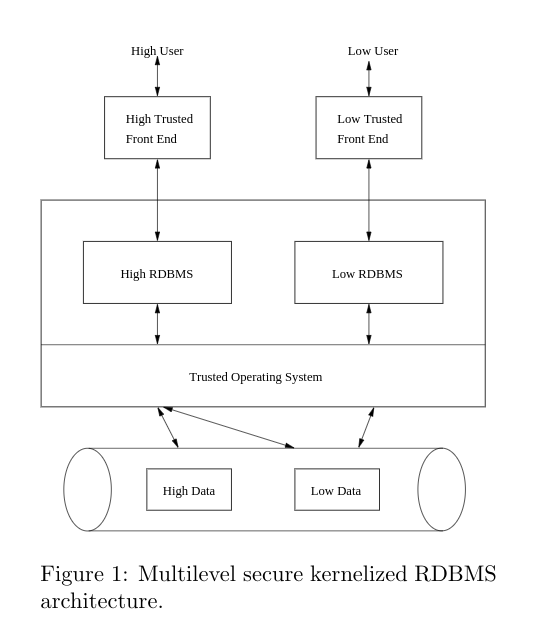
\includegraphics[width=0.8\textwidth]{assets/security/kernel.png}
    \caption{Ядерная архитектура}
    \label{fig:mesh01}
\end{figure}
На картинке изображена Ядерная архитектура, в которой одна РСУБД связана с уровнем безопасности «Высокий»,
а другая РСУБД связана с уровнем безопасности «Низкий».
РСУБД, связанная с уровнем безопасности «Высокий», имеет доступ как к фрагменту базы данных с высоким уровнем безопасности,
так и к фрагменту базы данных с низким уровнем безопасности. А РСУБД, ассоциированная с уровнем безопасности «Низкий»,
имеет доступ только к фрагменту базы данных с низким уровнем безопасности.
Преимущество этой архитектуры заключается в том, что данные на разных уровнях безопасности изолированы.
Еще одно преимущество состоит в том, что при условии, что надежная операционная система уже готова,
эта архитектура должна минимизировать количество времени и усилий для установки СУБД.
Однако эта архитектура приводит к дополнительным накладным расходам, поскольку доверенной
операционной системе необходимо разделять данные на разных уровнях безопасности при добавлении в базу данных,
а также может потребоваться совершать трудоемкие операции объединения данных с разных уровней безопасности.

\paragraph{Распределенные архитектуры}
Распределенная (или реплицированная) архитектура - это вариант ядерной архитектуры.
Он использует несколько копий доверенного интерфейса и СУБД, каждая из которых связана
со своим собственным хранилищем базы данных. В этой архитектурной схеме СУБД на уровне
безопасности содержит реплику каждого элемента данных, к которому субъект на уровне может получить доступ.
Таким образом, когда данные извлекаются повторно, СУБД извлекает их только из своей собственной базы данных.
Еще одно преимущество этой архитектуры состоит в том, что данные физически разделены на отдельные аппаратные базы данных.
Однако эта схема приводит к дополнительным накладным расходам, когда данные обновляются, поскольку различные
реплики должны быть синхронизированы.
\paragraph{Архитектура TrustedSubjects}
Архитектура TrustedSubjects - это схема, которая содержит надежную СУБД и надежную операционную систему.
Согласно этой архитектуре, политика обязательного контроля доступа обеспечивается самой СУБД.
Объекты базы данных (например, таблица) хранятся в объектах операционной системы (например, в файле) с наивысшим
уровнем безопасности. Таблица базы данных может содержать хранить строки с разными уровнями безопасности.
Такие строки различаются на основе их уровня безопасности, который явно сохраняется с каждой строкой.
Эта архитектура называется TrustedSubjects, потому что РСУБД имеет привилегию нарушать политику MAC
операционной системы при доступе к объектам базы данных. Например, когда пользователь с низким уровнем
безопасности запрашивает таблицу базы данных, к объекту операционной системы, в котором хранится эта таблица,
оказывается, что это является нарушением MAC-политики операционной системы. Но РСУБД способна возвращать пользователям
только те строки, для которых он или она авторизованы в соответствии с политикой MAC.
Преимущество этой архитектуры состоит в том, что СУБД имеет доступ ко всем уровням данных в одно и то же время,
что сводит к минимуму извлечение и обработку обновлений. Однако эта архитектура приводит к созданию специальной
РСУБД, которая требует разработки и проверки большого количества доверенного кода наряду с обычными функциями РСУБД.
Недостатком можно считать недостаточный уровень гарантии аппаратной изоляции объектов.
Также сложно доказать, что доверенное программное обеспечение, используемое для изоляции объектов
(например, потоков данных с разными уровнями безопасности), работает правильно, не допуская потока данных
с высоким уровнем безопасности для пользователей с низким уровнем безопасности.
\begin{figure}[H]
    \centering
    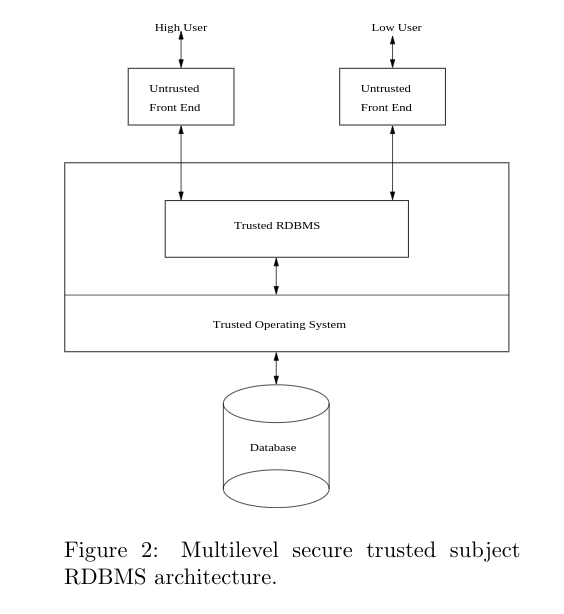
\includegraphics[width=0.8\textwidth]{assets/security/trusted.png}
    \caption{архитектура TrustedSubjects}
    \label{fig:mesh02}
\end{figure}

\subsection{Проектирование безопасных БД}
Разработать универсальную защищенную систему баз данных скорее всего нереально. При любом
разумном методе измерения уровня защищенности этот уровень является неубывающей функцией
от затрат на построение системы защиты. В любом практическом случае, когда существуют
ограничения на бюджет системы защиты, существует и некоторый предельный уровень
информационной безопасности, который теоретически может быть достигнут.

В настоящее время отсутствует общепринятая методология разработки защищенных
автоматизированных информационных систем и, в частности, систем баз данных. В подобных
случаях традиционно используется подход, основанный на анализе лучшего мирового опыта
решения некоторого класса проблем и формулировании руководящих принципов построения
соответствующих систем, концентрирующих накопленный опыт. Именно таким образом для проблемы
обеспечения безопасности информационных систем разрабатывался британский стандарт BS 7799
и созданный на его основе международный стандарт ISO 17799.

Анализ наиболее успешных решений в области обеспечения информационной безопасности баз данных
позволил сформулировать несколько полезных принципов, которыми можно руководствоваться
при проектировании систем защиты:
\begin{itemize}
	\item \textbf{Экономическая оправданность механизмов защиты.}
        Предписывает использование простейшего из всевозможных вариантов проекта, который
        обеспечивает достижение желаемой цели. Хотя этот принцип относится ко многим аспектам
        проектирования систем, он наиболее пригоден при разработке механизмов защиты, так как
        ошибки проектирования и реализации, которые ведут к неконтролируемым способам доступа
        к данным, могут быть не замечены в ходе нормального использования системы. Строгое
        соблюдение этого принципа приводит к применению на практике таких методов, как проверка
        «строка за строкой» программных средств и физическая проверка аппаратных средств,
        реализующих механизмы защиты.

    \item \textbf{Открытое проектирование.}
        Технология систем защиты не должна базироваться на «секретных» алгоритмах. Этот принцип
        широко используется при проектировании безопасных систем и сетей связи. Высокое качество
        систем защиты обеспечивается не недостатком знаний у возможных нарушителей,
        а использованием широко опробованных (как правило, открытых) стандартов и правильной
        организацией управления ключевой информацией. Использование алгоритмов, основанных на
        открытых стандартах в области информационной безопасности, повышает степень доверия
        пользователей к системе защиты и формирует правильную психологическую установку на
        необходимость внимательности и аккуратности при работе с ключевой информацией.

	\item \textbf{Распределение полномочий между различными субъектами в соответствии с правилами организации.}
        Состоит в том, что для критически важных приложений целесообразно использовать многокомпонентные
        схемы доступа к данным. То есть для выполнения соответствующей операции необходимо провести
        аутентификацию нескольких ее обязательных участников. Физический аналог этого принципа можно
        наблюдать в конструкциях банковских сейфов, когда для того, чтобы открыть сейф, необходимо наличие
        двух ключей, которые обычно хранятся у различных людей. Ясно, что механизмы защите, требующие двух
        ключей для доступа к информации, являются более устойчивыми, чем механизмы, которые разрешают доступ
        на основе предъявления единственного ключа. В то же время подобные многокомпонентные процедуры требуют
        больших затрат и, как правило, более сложных процедур управления ключами (включая хранение резервной
        копии). При проектировании многокомпонентных схем доступа за прообраз берется существующая в
        организации практика. Действительно, переход в автоматизированном контуре на более сложные,
        чем использовались «в доавтоматизированную эру», технологии может вызвать психологический дискомфорт
        и различные формы скрытого саботажа системы.

    \item \textbf{Минимально возможные привилегии для пользователей и администраторов.}
        Предписывает, чтобы каждый пользователь (процесс) системы оперировали с данными, используя наименьший
        из возможных набор привилегий, необходимых для выполнения конкретной функции. Применение данного
        принципа нацелено на минимизацию ущерба, который может быть нанесен в случае сбоя, ошибки программного
        обеспечения или компрометации элементов системы защиты данных. Принцип минимальных привилегий,
        используемый при создании пользователей Oracle, — пример реализации этого принципа. Использование
        точек входа SYSTEM и, особенно, SYS должно быть предметом особого регламента. Хорошей практикой
        является использование администратором безопасности нескольких точек входа: обычной, с набором
        привилегий, достаточным для выполнения основных работ, и особой (типа SYSTEM), используемой только
        при возникновении необходимости выполнения действий, требующих высоких привилегий.

    \item \textbf{Управляемость системы при возникновении отказов и сбоев.}
        Проектирование информационной системы, реализованной на базе СУБД, должно осуществляться в предположении,
        что ошибки операционной системы и СУБД, а также сбои аппаратуры неизбежны. При создании системы
        возможность реализации таких событий должна быть учтена: при проектировании процедур и функций должны
        быть обработаны все исключительные ситуации, при обработке данных, содержащих конфиденциальную информацию,
        должны быть минимизированы риски восстановления этих данных по дампам оперативной памяти и содержимому
        временных файлов и т. п. Также должны быть разработаны документы, регламентирующие действия участников
        процесса обработки данных (как пользователей, так и обслуживающего персонала) при возникновении нештатных
        ситуаций. Персонал должен проходить регулярные инструктажи и тренинги по обучению действиям в нештатных
        ситуациях, с иерархией передачи данных.

    \item \textbf{Психологическая приемлемость работы средств защиты данных.}
        Взаимодействие людей с системой (и подсистемой защиты) не должно быть сложным. Пользователи должны
        шаблонно и автоматически применять имеющиеся механизмы защиты. Чрезмерное усложнение механизмов защиты
        может вызывать их внутреннее неприятие и побуждать к использованию различных форм скрытого саботажа.
        Осознанное принятие используемых средств и методов обеспечения информационной безопасности и оценка
        комплекса применяемых мер как необходимых приводит к уменьшению числа ошибок пользователей. В этом случае
        аномальное поведение потенциального нарушителя становится более заметным и проще устанавливается.
        Принцип психологической приемлемости является важным при выборе процедур аутентификации и модели
        управления доступом.
\end{itemize}

\subsubsection{Фазы проектирования безопасных БД (по DoD)}

Министерство обороны (Department of Defence) предложило методологию проектирования, использования и вывода
системы из эксплуатации безопасных информационных систем, в том числе безопасных БД. Стадии жизненного
цикла информационной системы, наиболее часто используемые Министерством обороны, показаны на рис. 6.

\begin{figure}[H]
    \centering
    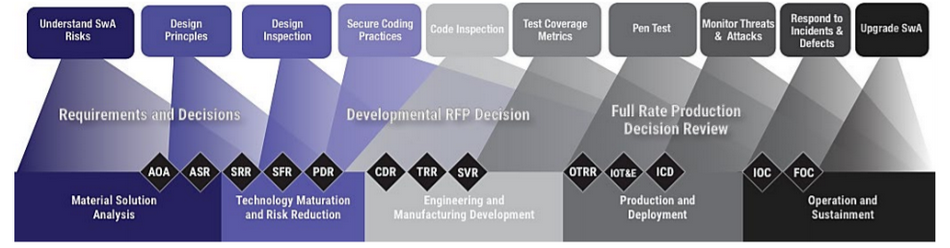
\includegraphics[width=0.8\textwidth]{assets/security/pic1.png}
    \caption{Стадии жизненного цикла по DoD}
    \label{fig:mesh03}
\end{figure}

Как показано на рис. 6, основная часть жизненного цикла информационной системы включает пять этапов: работа
с требованиями, проектирование архитектуры информационной системы, реализация информационной системы,
тестирование и введение в эксплуатацию. На этапе требований происходит анализ требований заказчика,
формулирование политик безопасности и требований к разрабатываемой информационной системе. На этапе проектирования
архитектуры на основе набора требований, представленного в функциональной форме, составляется концептуальная
модель системы, на основе концептуальной – логическая, на основе логической – физическая.

\subsubsection{Предварительный анализ}

Анализ требований является одним из первых этапов процесса системного проектирования и в некоторой степени
представляет собой интерфейс между внутренними действиями и внешними источниками, предоставляющими входные
данные. В процессе анализа требований исследуются, оцениваются и преобразуются внешние входные данные в
набор функциональных требований, политик безопасности и требований к производительности, которые будут являться
основой для последующего концептуального, логического и физического проектирований. Цель анализа требований –
определение требований к системе.

Анализ миссии системы, анализ среды использования системы определяют потребности клиента и формулируют их в терминах,
которые могут быть использованы для определения функций системы, требований к производительности или проектных
ограничений. Такой анализ определяет функциональные требования к системе, уточняет требования к характеристикам
или проектированию. По мере продвижения этой деятельности исходные предположения и выводы сверяются с меняющимися
деталями. Обычно это приводит к некоторому изменению исходного мышления заказчика, может даже отражаться на его
потребностях, некоторые из которых могут оказаться непрактичными или чрезмерно дорогостоящими.

Результатом анализа требований является набор функциональных определений верхнего уровня и сопутствующих требований
к производительности и архитектуре, которые становятся отправной точкой концептуального проектирования. Анализ
требований проводится итеративно, цикл анализа требований служит для уточнения требований и инициирования
повторной оценки, чтобы определить, насколько жесткими являются требования к элементам системы. Позже подробные
характеристики системы сравниваются с установленными требованиями, чтобы убедиться, что они выполняются.
На этом этапе обычно мало изменений в требованиях из-за обратной связи проверки, но иногда некоторые незначительные
изменения рассматриваются, когда отдача значительна.

\subsubsection{Требования и политики безопасности}

Политика безопасности — это совокупность норм и правил, определяющих принятые в организации меры по обеспечению
безопасности информации, связанной с деятельностью организации. Только человек, четко осознающий цели организации
и условия ее функционирования, может определить, какую информацию необходимо защищать и насколько существенными
могут стать потери от несанкционированного распространения, искажения или разрушения информации. После того как
политика безопасности определена, должен решаться вопрос о технологии ее реализации в автоматизированном контуре.
Для реализации сформулированных в терминах естественного языка правил и норм политики безопасности необходимо
использовать (или разработать) некоторую формальную модель, которая допускает эффективное программирование на
каком-либо формальном языке. Наибольшее распространение в настоящее время получили две базовые модели безопасности
данных: дискреционная и мандатная \autocite{shveikin}.

Цель формализации политики безопасности для информационной системы — ясное изложение взглядов руководства
организации на существо угроз информационной безопасности организации и технологий обеспечения безопасности ее
информационных ресурсов. Политика безопасности обычно состоит из двух частей: общих принципов и конкретных правил
работы с информационными ресурсами, то есть требований, и, в частности, с базами данных для различных категорий
пользователей. Политика безопасности – это всегда некоторый компромисс между желаемым уровнем защищенности ресурсов
информационной системы, удобством работы с системой и затратами средств, выделяемых на ее эксплуатацию \autocite{shveikin}.

Политика безопасности должна быть оформлена документально на нескольких уровнях управления. На уровне управляющего
высшего звена руководства должен быть подготовлен и утвержден документ, в котором определены цели политики
безопасности, структура и перечень решаемых задач и ответственные за реализацию политики. Основной документ
должен быть детализирован администраторами безопасности информационных систем (управляющими среднего звена)
с учетом принципов деятельности организации, соотношения важности целей, и наличия ресурсов. Детальные решения
должны включать ясные определения методов защиты технических и информационных ресурсов, а также инструкции,
определяющие поведение сотрудников в конкретных ситуациях \autocite{shveikin}.

В руководстве по компьютерной безопасности, разработанном национальным институтом стандартов и технологий
США (National Institute of Standards and Technology — NIST), рекомендовано включать в описание
политики безопасности следующие разделы  \autocite{nurzhanov}:
\begin{itemize}
	\item \textbf{Предмет политики.}
        В разделе должны быть определены цели и причины разработки политики, область ее применения
        в конкретном фрагменте системы документооборота организации. Должны быть ясно сформулированы
        задачи, решаемые с использованием информационных систем, которые затрагивает данная политика.
        При необходимости могут быть сформулированы термины и определения, используемые в остальных разделах.

    \item \textbf{Описание позиции организации.}
        В этом разделе необходимо ясно описать характер информационных ресурсов организации, перечень
        допущенных к информационным ресурсам лиц и процессов и порядок получения доступа к информационным
        ресурсам организации.

    \item \textbf{Применимость.}
        В разделе может быть уточнен порядок доступа к данным ИС, определены ограничения или технологические
        цепочки, применяемые при реализации политики безопасности.

    \item \textbf{Роли и обязанности.}
        В разделе определяются ответственные должностные лица и их обязанности в отношении разработки и
        внедрения различных элементов политики. Обычно определяются обязанности администратора безопасности
        данных (отвечает за содержательную сторону предоставления доступа к информационным ресурсам организации),
        администратора баз данных (определяет техническую реализацию механизмов разграничения доступа),
        администратора локальной сети, операторов.

    \item \textbf{Соблюдение политики.}
        В разделе описываются права и обязанности пользователей ИС. Необходимо явное описание и документированное
        знакомство пользователей с перечнем недопустимых действий при осуществлении доступа к информационным ресурсам
        организации и наказания за нарушения режимных требований. Должна быть ясно определена технология фиксации
        фактов нарушения политики безопасности и применения административных мер воздействия к нарушителям.
\end{itemize}

Для эффективной реализации политика безопасности должна быть понятной всем пользователям информационных
систем организации. Возможна подготовка презентаций и проведение семинаров с разъяснением основных положений
и практических технологий реализации политики безопасности. Новые сотрудники организации должны быть ознакомлены
или обучены конкретным правилам и технологиям доступа к ресурсам ИС, реализованным в соответствии с принятой
политикой безопасности. Целесообразно проводить контрольные проверки действий сотрудников с обсуждением результатов \autocite{shveikin}.

Эффективное проведение политики безопасности возможно только, если она согласована с существующими приказами
и общими задачами организации. Основным способом координации политики безопасности с действующими нормами
организации является ее согласование с заинтересованными подразделениями в ходе разработки.

Комплект документов, представляющий основные решения организации по реализации политики безопасности,
должен включать \autocite{nurzhanov}:
\begin{itemize}
    \item
        документацию, определяющую используемые подходы к оцениванию и управлению рисками для
        организации в целом и при необходимости конкретных подразделений;

    \item
        обоснование принятых решений по выбору средств защиты для рассматриваемой информационной системы;

    \item
        формальное описание процедуры определения допустимого уровня остаточного риска;

    \item
        директиву, определяющую процедуру проверки режима информационной безопасности и журналов,
        в которых фиксируются результаты проверки (документы необходимы для осуществления проверки
        эффективности реализации средств обеспечения информационной безопасности, осуществления
        их контроля качества и правильности использования);

    \item
        документацию, регламентирующую процессы обслуживания и администрирования информационных систем;

    \item
        документацию по подготовке периодических проверок по оцениванию и управлению рисками;

    \item
        документ «Ведомость соответствия», включающий сведения по организации системы управления
        информационной безопасностью и регистрации средств управления безопасностью;

    \item
        контрмеры для противодействия выявленным рискам.
\end{itemize}

Успех проведения в жизнь политики безопасности больше зависит от усилий и опытности людей, реализующих политику,
чем от сложных программно-технических средств контроля.

\subsubsection{Концептуальное проектирование}

Цель этапа концептуального проектирования – создание концептуальной модели данных исходя из представлений
пользователей о предметной области. Для ее достижения выполняется ряд последовательных процедур \autocite{oscerko}.
\begin{enumerate}
	\item \textbf{Определение сущностей и их документирование.}
	Для идентификации сущностей определяются объекты, которые существуют независимо от других. Такие объекты
	являются сущностями. Каждой сущности присваивается осмысленное имя, понятное пользователям. Имена и
	описания сущностей заносятся в словарь данных. Если возможно, то устанавливается ожидаемое количество
	экземпляров каждой сущности.
	
	Предположим, что проектируется база данных, предназначенная для хранения информации о деятельности некоторого банка. Этот банк
	имеет филиалы. Филиалы управляются менеджерами. Клиенты имеют в филиалах счета разных типов – текущие, срочные, до востребования, депозитные, карточные.
	Филиалы обрабатывают эти счета. Описываемую предметную область назовем БАНК, в ней могут быть выделены 4 сущности: ФИЛИАЛ, МЕНЕДЖЕР, СЧЕТ, КЛИЕНТ.
	\begin{itemize}
		
		\item ФИЛИАЛ: номер филиала, адрес филиала;
		
		\item МЕНЕДЖЕР: номер менеджера, стаж работы по специальности;
		
		\item СЧЕТ: номер счета, тип счета, дата открытия счета, капитализация (Да/Нет), остаток на счете;
		
		\item КЛИЕНТ: номер клиента, ФИО клиента, адрес клиента, подпись клиента.
		
	\end{itemize}
	
	\item \textbf{Определение связей между сущностями и их документирование.}
	Определяются только те связи между сущностями, которые необходимы для удовлетворения требований к проекту
	базы данных. Устанавливается тип каждой из них. Выявляется класс принадлежности сущностей. Связям
	присваиваются осмысленные имена, выраженные глаголами. Развернутое описание каждой связи с указанием ее
	типа и класса принадлежности сущностей, участвующих в связи, заносится в словарь данных.
	
	В рассматриваемой предметной области БАНК можно выделить 3 связи:
	\begin{itemize}
		
		\item МЕНЕДЖЕР управляет ФИЛИАЛом
		
		\item ФИЛИАЛ обрабатывает СЧЕТ
		
		\item КЛИЕНТ имеет СЧЕТ
		
	\end{itemize}
	
	\item \textbf{Создание ER-модели предметной области.}
	Для представления сущностей и связей между ними используются ER-диаграммы. На их основе создается единый
	наглядный образ моделируемой предметной области – ER-модель предметной области.
	
	На диаграмме сущность изображается прямоугольником, в
	котором указывается ее имя. А связь ромбом. Так же важен тип связи(1:1, 1:M, M:N). Рассмотрим их подробнее:
	\begin{itemize}
		\item 1:1(один к одному): примером такой связи служит <<МЕНЕДЖЕР управляет ФИЛИАЛом>>, так как МЕНЕДЖЕР управляет только одним ФИЛИАЛом, а ФИЛИАЛ имеет только одного МЕНЕДЖЕРа;
		
		\item 1:M(один ко многим): примером такой связи служит <<ФИЛИАЛ  обрабатывает СЧЕТ>>, так как СЧЕТ обрабатывается только одним ФИЛИАЛом, а ФИЛИАЛ может обрабатывать более одного СЧЕТа;
		
		\item  M:N(многие ко многим): примером такой связи служит <<КЛИЕНТ ИМЕЕТ СЧЕТ>>, так как СЧЕТ может быть совместным и им могут пользоваться сразу несколько КЛИЕНТов, а КЛИЕНТ может завести более одного СЧЕТа;
	\end{itemize}
	\begin{figure}[H]
		\centering
		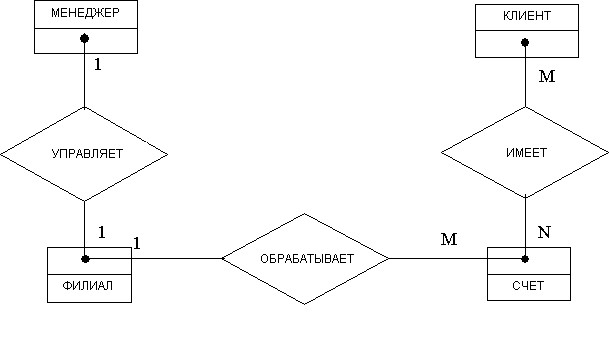
\includegraphics[width=0.8\textwidth]{assets/security/pic25.png}
		\caption{ER-модель предметной области БАНК}
		\label{fig:mesh28}
	\end{figure}
	
	\item \textbf{Определение атрибутов и их документирование.}
	Выявляются все атрибуты, описывающие сущности созданной ER-модели. Каждому атрибуту присваивается осмысленное
	имя, понятное пользователям. О каждом атрибуте в словарь данных помещаются следующие сведения:
	\begin{itemize}
		\item имя атрибута и его описание;
		
		\item тип и размерность значений;
		
		\item значение, принимаемое для атрибута по умолчанию (если такое имеется);
		
		\item может ли атрибут иметь NULL-значения;
		
		\item является ли атрибут составным, и если это так, то из каких простых атрибутов он состоит.
		Например, атрибут <<Ф.И.О. клиента>> может состоять из простых атрибутов <<Фамилия>>, <<Имя>>,
		<<Отчество>>, а может быть простым, содержащим единые значения, как-то <<Сидорский Евгений
		Михайлович>>. Если пользователь не нуждается в доступе к отдельным элементам <<Ф.И.О.>>,
		то атрибут представляется как простой;
		
		\item является ли атрибут расчетным, и если это так, то как вычисляются его значения.
	\end{itemize}
	
	\item \textbf{Определение значений атрибутов и их документирование.}
	Для каждого атрибута сущности, участвующей в ER-модели, определяется набор допустимых значений и ему
	присваивается имя. Например, атрибут <<Тип счета>> может иметь только значения <<депозитный>>, <<текущий>>,
	<<до востребования>>, <<карт-счет>>. Обновляются записи словаря данных, относящиеся к атрибутам, – в них
	заносятся имена наборов значений атрибутов.
	
	\item \textbf{Определение первичных ключей для сущностей и их документирование.}
	На этом шаге руководствуются определением первичного ключа – как атрибута или набора атрибутов сущности,
	позволяющего уникальным образом идентифицировать ее экземпляры. Сведения о первичных ключах помещаются
	в словарь данных.
	
	\item \textbf{Обсуждение концептуальной модели данных с конечными пользователями.}
	Концептуальная модель данных представляется ER-моделью с сопроводительной документацией, содержащей
	описание разработанной модели данных. Если будут обнаружены несоответствия предметной области, то в
	модель вносятся изменения  до тех пор, пока пользователи не подтвердят, что предложенная им модель
	адекватно отображает их личные представления.
\end{enumerate}

\subsubsection{Логическое  проектирование}

Цель этапа логического проектирования – преобразование концептуальной модели на основе выбранной модели данных
в логическую модель, не зависимую от особенностей используемой в дальнейшем СУБД для физической реализации базы
данных. Для ее достижения выполняются следующие процедуры \autocite{oscerko}:
\begin{enumerate}
    \item \textbf{Выбор модели данных.}
        Чаще всего выбирается реляционная модель данных в связи с наглядностью табличного представления данных
        и удобства работы с ними.

    \item \textbf{Определение набора таблиц исходя из ER-модели и их документирование.}
        Для каждой сущности ER-модели создается таблица. Имя сущности – имя таблицы. Причем каждому атрибуту
        сущности соответствует столбец таблицы. Правила генерации таблиц из ER-диаграмм опираются на два основных
        фактора – тип связи и класс принадлежности сущности. Устанавливаются связи между таблицами посредством
        механизма первичных и внешних ключей. Структуры таблиц и установленные связи между ними документируются.

        Изложим правила генерации таблиц из ER-диаграмм, используя пример ER-модели предметной
        области БАНК, представленной на рис. 7, со следующими наборами атрибутов сущностей предметной области БАНК,
        представленными на рис. 8.

    \begin{figure}[H]
        \centering
        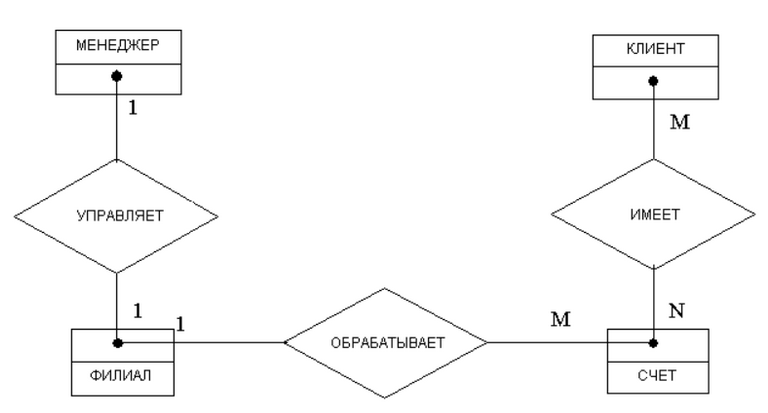
\includegraphics[width=0.8\textwidth]{assets/security/pic2.png}
        \caption{Пример ER-модели предметной области БАНК}
        \label{fig:mesh04}
    \end{figure}

    \begin{figure}[H]
        \centering
        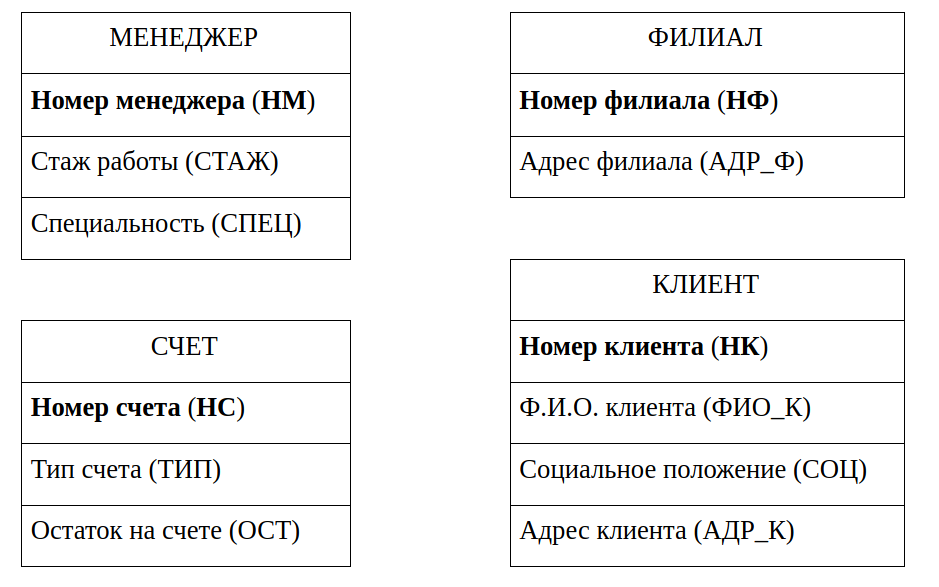
\includegraphics[width=0.8\textwidth]{assets/security/pic3.png}
        \caption{Наборы атрибутов сущностей предметной области БАНК}
        \label{fig:mesh05}
    \end{figure}

    Для связи типа 1:1 существуют три отдельных правила формирования предварительных таблиц из ER-диаграмм.

    \underline{Правило 1}

    Если связь типа 1:1 и класс принадлежности обеих сущностей является обязательным, то необходима только одна
    таблица. Первичным ключом этой таблицы может быть первичный ключ любой из двух сущностей.

    На ER-диаграмме связи 1:1, класс принадлежности сущностей МЕНЕДЖЕР, ФИЛИАЛ является обязательным. Тогда согласно
    правилу 1 должна быть сгенерирована одна таблица следующей структуры:

    \begin{figure}[H]
        \centering
        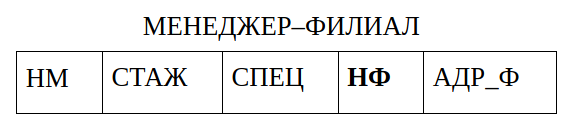
\includegraphics[width=100mm]{assets/security/pic4.png}
        \label{fig:mesh06}
    \end{figure}

    Первичным ключом этой таблицы может быть и первичный ключ сущности МЕНЕДЖЕР – НМ.

    \underline{Правило 2}

    Если связь типа 1:1 и класс принадлежности одной сущности является обязательным, а другой – необязательным,
    то необходимо построить таблицу для каждой сущности. Первичный ключ сущности должен быть первичным ключом
    соответствующей таблицы. Первичный ключ сущности, для которой класс принадлежности является необязательным,
    добавляется как атрибут в таблицу для сущности с обязательным классом принадлежности.

    Представим, что на ER-диаграмме связи 1:1, изображенной на рис. 7, класс принадлежности сущности МЕНЕДЖЕР
    будет обязательный, а сущности ФИЛИАЛ – необязательный. Тогда согласно правилу 2 должны быть сгенерированы
    две таблицы следующей структуры:

    \begin{figure}[H]
        \centering
        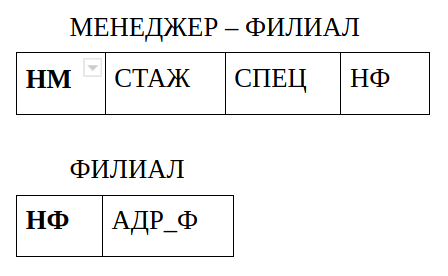
\includegraphics[width=100mm]{assets/security/pic5.png}
        \label{fig:mesh07}
    \end{figure}

    Сущность с необязательным классом принадлежности (ФИЛИАЛ) именуется родительской, а с обязательным (МЕНЕДЖЕР)
    – дочерней. Первичный ключ родительской сущности (НФ), помещаемый в таблицу, представляющую дочернюю сущность,
    называется внешним ключом родительской сущности. Связь между указанными таблицами устанавливается путем связи
    первичного и внешнего ключа и имеет вид:

    \begin{figure}[H]
        \centering
        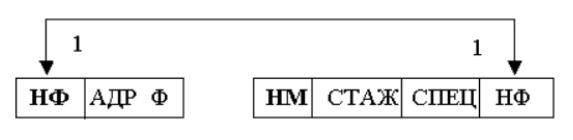
\includegraphics[width=0.8\textwidth]{assets/security/pic6.png}
        \label{fig:mesh08}
    \end{figure}

    Примечание. Если внешний ключ представляет связь 1:1, то должны быть запрещены его дублирующие значения.

    \underline{Правило 3}

    Если связь типа 1:1 и класс принадлежности обеих сущностей является необязательным, то необходимо построить
    три таблицы – по одной для каждой сущности и одну для связи. Первичный ключ сущности должен быть первичным
    ключом соответствующей таблицы. Таблица для связи среди своих атрибутов должна иметь ключи обеих сущностей.

    Представим, что на ER-диаграмме связи 1:1, изображенной на рис. 7, класс принадлежности сущностей МЕНЕДЖЕР,
    ФИЛИАЛ будет необязательный. Тогда согласно правилу 3 должны быть сгенерированы три таблицы следующей структуры:

    \begin{figure}[H]
        \centering
        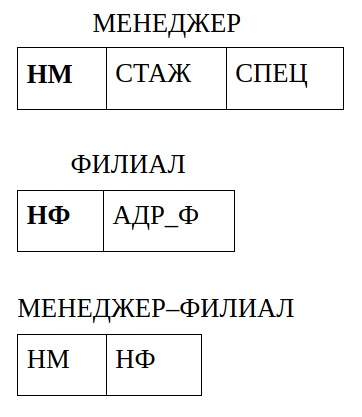
\includegraphics[width=100mm]{assets/security/pic7.png}
        \label{fig:mesh09}
    \end{figure}

    При этом осуществляется декомпозиция связи 1:1 на две связи 1:1 следующим образом:

    \begin{figure}[H]
        \centering
        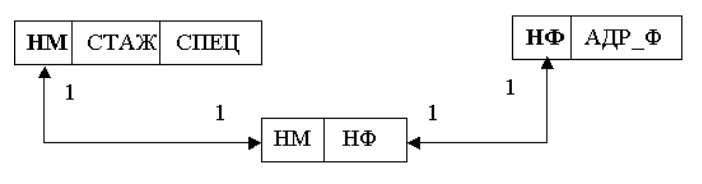
\includegraphics[width=0.8\textwidth]{assets/security/pic8.png}
        \label{fig:mesh10}
    \end{figure}

    Для связи типа 1:М существуют только два правила. Выбор одного из них зависит от класса принадлежности
    сущности на стороне M. Класс принадлежности сущности на стороне 1 не влияет на выбор.

    \underline{Правило 4}

    Если связь типа 1:М и класс принадлежности сущности на стороне М является обязательным, то необходимо
    построить таблицу для каждой сущности. Первичный ключ сущности должен быть первичным ключом соответствующей
    таблицы. Первичный ключ сущности на стороне 1 добавляется как атрибут в таблицу для сущности на стороне М.

    На ER-диаграмме связи 1:М, представленной на рис. 7, класс принадлежности сущности СЧЕТ является обязательным.
    Тогда согласно правилу 4 должны быть сгенерированы две таблицы следующей структуры:

    \begin{figure}[H]
        \centering
        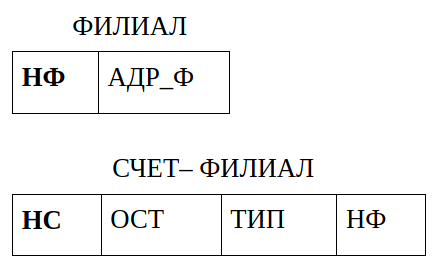
\includegraphics[width=100mm]{assets/security/pic9.png}
        \label{fig:mesh11}
    \end{figure}

    Связь между указанными таблицами будет иметь вид:

    \begin{figure}[H]
        \centering
        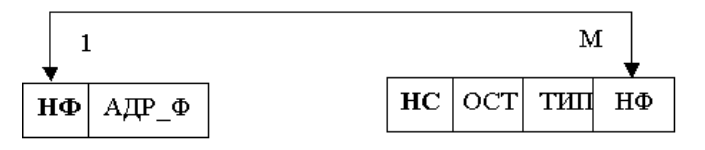
\includegraphics[width=0.8\textwidth]{assets/security/pic10.png}
        \label{fig:mesh12}
    \end{figure}

    Примечание. Если внешний ключ представляет связь 1:М, то должны быть разрешены его дублирующие значения.

    \underline{Правило 5}

    Если связь типа 1:М и класс принадлежности сущности на стороне М является необязательным,
    то необходимо построить три таблицы – по одной для каждой сущности и одну для связи. Первичный ключ сущности
    должен быть первичным ключом соответствующей таблицы. Таблица для связи среди своих атрибутов должна
    иметь ключи обеих сущностей.

    Представим, что на ER-диаграмме связи 1:М, изображенной на рис. 7, класс принадлежности сущности СЧЕТ
    является необязательным. Тогда согласно правилу 5 должны быть сгенерированы три таблицы следующей структуры:

    \begin{figure}[H]
        \centering
        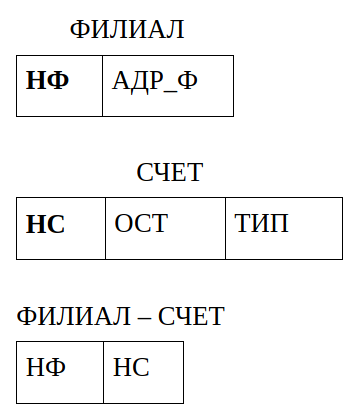
\includegraphics[width=100mm]{assets/security/pic11.png}
        \label{fig:mesh13}
    \end{figure}

    При этом осуществляется декомпозиция связи 1:М на две связи – 1:М и 1:1 – следующим образом

    \begin{figure}[H]
        \centering
        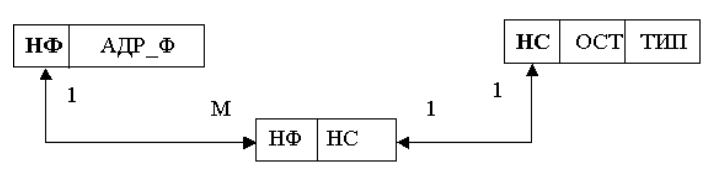
\includegraphics[width=0.8\textwidth]{assets/security/pic12.png}
        \label{fig:mesh14}
    \end{figure}

    Для связи типа М:N класс принадлежности сущности не имеет значения.

    \underline{Правило 6}

    Если связь типа М:N, то необходимо построить три таблицы – по одной для каждой сущности и одну для связи.
    Первичный ключ сущности должен быть первичным ключом соответствующей таблицы. Таблица для связи среди своих
    атрибутов должна иметь ключи обеих сущностей.

    ER-диаграмма связи М:N имеется на рис. 7. Согласно правилу 6 на основе этой ER-диаграммы должны быть
    сгенерированы три таблицы следующей структуры:

    \begin{figure}[H]
        \centering
        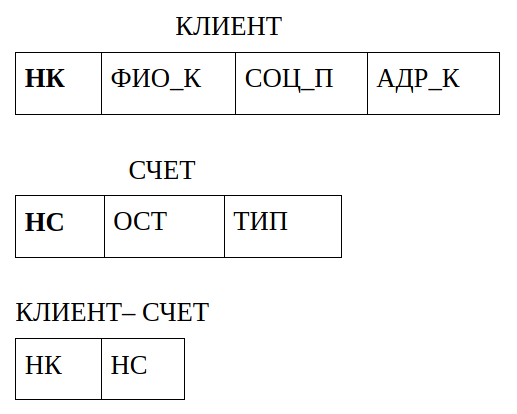
\includegraphics[width=100mm]{assets/security/pic13.png}
        \label{fig:mesh15}
    \end{figure}

    При этом осуществляется декомпозиция связи М:N на две связи 1:М следующим образом:

    \begin{figure}[H]
        \centering
        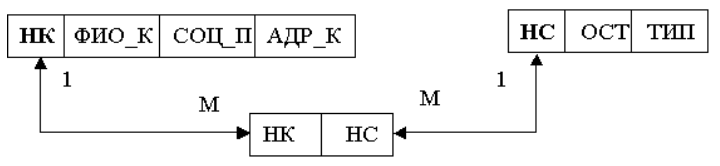
\includegraphics[width=0.8\textwidth]{assets/security/pic14.png}
        \label{fig:mesh16}
    \end{figure}

    В таблице КЛИЕНТ–СЧЕТ клиенту, имеющему, например, три счета будут соответствовать три строки
    с одним и тем же номером клиента. А счет, у которого, например, два владельца, представляется двумя
    строками с различными номерами клиентов, владеющими этим счетом.

    К ER-модели предметной области БАНК, представленной на рис. 7, применимы правила 1, 4, 6. Связь МЕНЕДЖЕР
    – ФИЛИАЛ представляется (согласно правилу 1) одной таблицей А:

    \begin{figure}[H]
        \centering
        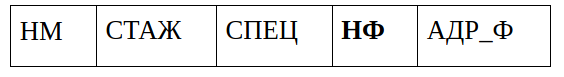
\includegraphics[width=0.8\textwidth]{assets/security/pic15.png}
        \label{fig:mesh17}
    \end{figure}

    Связь ФИЛИАЛ – СЧЕТ  представляется (согласно правилу 4) связью:

    \begin{figure}[H]
        \centering
        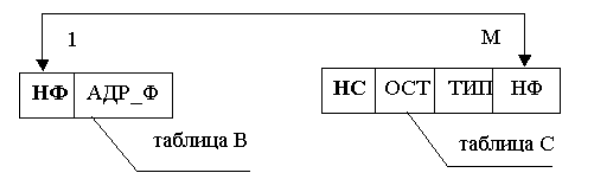
\includegraphics[width=0.8\textwidth]{assets/security/pic16.png}
        \label{fig:mesh18}
    \end{figure}

    Связь КЛИЕНТ – СЧЕТ представляется (согласно правилу 6) связью:

    \begin{figure}[H]
        \centering
        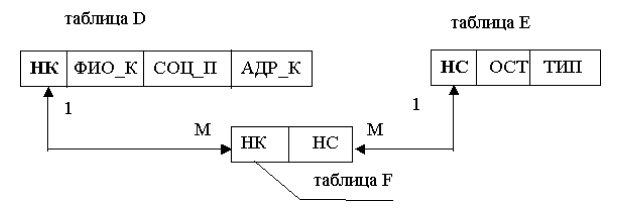
\includegraphics[width=0.8\textwidth]{assets/security/pic17.png}
        \label{fig:mesh19}
    \end{figure}

    Анализ состава атрибутов полученных таблиц A, B, C, D, E, F показывает, что таблица В является составной
    частью таблицы А, таблица Е – составной частью таблицы С. Поэтому таблицы В, Е можно исключить из рассмотрения.
    Оставшиеся таблицы А, С, D, F можно связать посредством связи первичных и внешних ключей.
    В результате получим реляционную модель для ER-модели предметной области БАНК.

    \item \textbf{Нормализация таблиц.}
        Для правильного выполнения нормализации проектировщик должен глубоко изучить семантику и особенности
        использования данных. На этом шаге он проверяет корректность структуры таблиц, созданных на предыдущем
        шаге, посредством применения к ним процедуры нормализации. Она заключается в приведении каждой из таблиц,
        по крайней мере, к 3НФ. В результате нормализации получается очень гибкий проект базы данных,
        позволяющий легко вносить в нее нужные расширения.

        Нормализация таблиц - процесс, позволяющий минимизировать избыточность данных. Чтобы пояснить этот процесс,
        будем исходить из описания предметной области БАНК, представленного на рис. 7, и предположения, что на его
        основе была разработана база данных, состоящая из следующих двух таблиц:

    \begin{figure}[H]
        \centering
        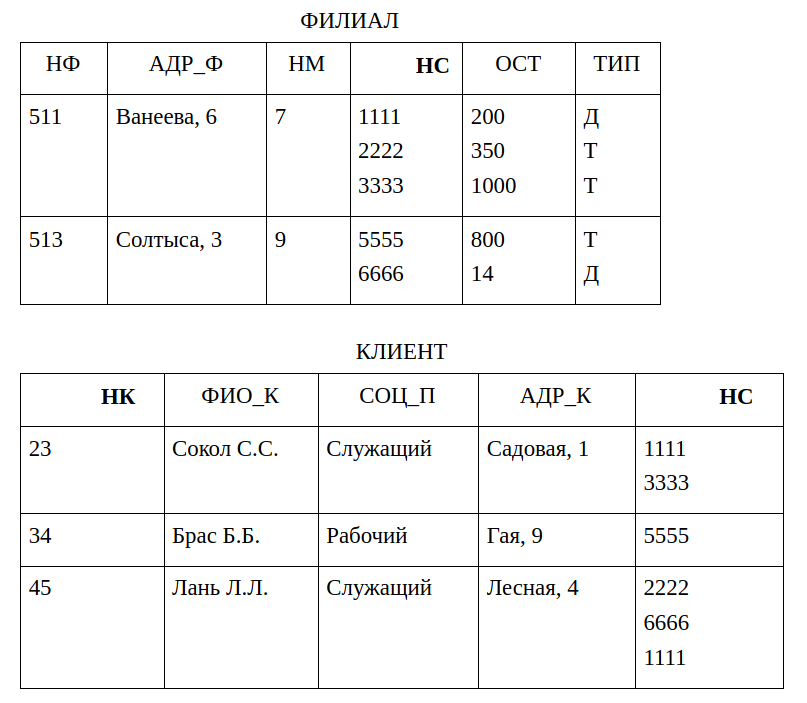
\includegraphics[width=0.8\textwidth]{assets/security/pic18.png}
        \label{fig:mesh20}
    \end{figure}

    \underline{1 нормальная форма (1НФ)}

    Таблица находится в 1НФ, если все ее поля содержат только простые неделимые значения.

    Таблицы ФИЛИАЛ и КЛИЕНТ не удовлетворяют требованиям 1НФ. Для приведения их к 1НФ в них надо вставить новые
    записи следующим образом:

    \begin{figure}[H]
        \centering
        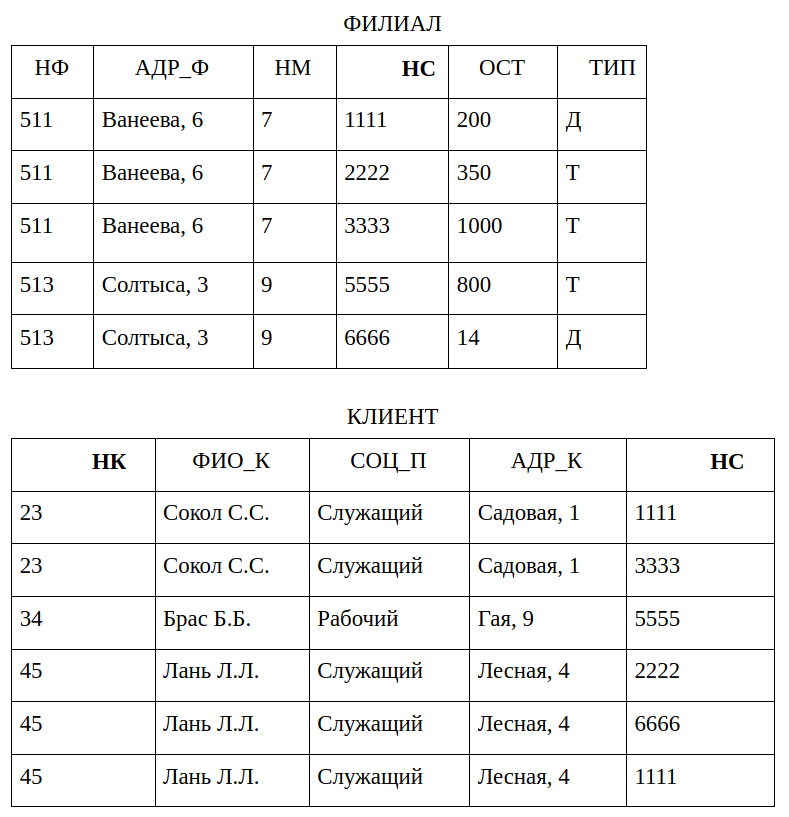
\includegraphics[width=0.8\textwidth]{assets/security/pic19.png}
        \label{fig:mesh21}
    \end{figure}

    Но полученные таблицы неэффективны, так как содержат много избыточной информации. Необходимо их привести к 2НФ.

    \underline{2 нормальная форма (2НФ)}

    Таблица находится в 2НФ, если она удовлетворяет требованиям 1НФ и неключевые поля функционально полно
    зависят от первичного ключа.

    Функциональная зависимость – это понятие, отображающее определенную семантическую связь между полями таблицы.
    Неключевое поле А функционально полно зависит от первичного ключа, если:
    \begin{enumerate}
        \item оно функционально зависит от первичного ключа, т.е. каждой комбинации значений полей первичного
        ключа соответствует одно и только одно значение поля А;

        \item не существует функциональной зависимости А ни от какого подмножества полей первичного ключа
        (в противном случае А находится в частичной функциональной зависимости от первичного ключа).
    \end{enumerate}

    В таблице КЛИЕНТ неключевые поля ФИО\_К, СОЦ\_П, АДР\_К функционально зависят от ключа (НК, НС). Кроме того,
    они функционально зависят от подмножества ключа – НК. Следовательно, неключевые поля ФИО\_К, СОЦ\_П, АДР\_К
    находятся в частичной функциональной зависимости от первичного ключа (НК, НС) и нарушаются требования 2НФ.
    Эти поля надо из таблицы КЛИЕНТ удалить. Полученную в результате этого таблицу назовем КЛИЕНТ–СЧЕТ, которая
    имеет вид:

    \begin{figure}[H]
        \centering
        \includegraphics[width=40mm]{assets/security/pic20.png}
        \label{fig:mesh22}
    \end{figure}

    Эта таблица удовлетворяет требованиям 2НФ.

    Удаленные неключевые поля помещаются в новую таблицу совместно с подмножеством НК, от которого они зависят.
    И это подмножество будет первичным ключом новой таблицы КЛИЕНТ вида:

    \begin{figure}[H]
        \centering
        \includegraphics[width=0.8\textwidth]{assets/security/pic21.png}
        \label{fig:mesh23}
    \end{figure}

    Новая таблица КЛИЕНТ также удовлетворяет требованиям 2НФ. Ее неключевые поля функционально полно зависят
    от первичного ключа.

    Полученные таблицы не содержат избыточной информации, и нет основания приводить их к 3НФ. Таблица ФИЛИАЛ
    удовлетворяет требованиям 2НФ, так как ее неключевые поля НФ, АДР\_Ф, НМ, ОСТ, ТИП функционально полно
    зависят от первичного ключа. Но в таблице ФИЛИАЛ повторяется информация о филиале для всех счетов,
    обрабатываемых им. Поэтому ее надо привести к 3НФ.

    \underline{3 нормальная форма (3НФ)}

    Таблица находится в 3НФ, если она удовлетворяет требованиям 2НФ и не содержит транзитивных зависимостей.

    Транзитивной зависимостью называется функциональная зависимость между неключевыми полями. В таблице ФИЛИАЛ
    она наблюдается. Следовательно, нарушаются требования 3НФ. Из таблицы ФИЛИАЛ надо удалить поля, участвующие
    в этой транзитивной зависимости, – АДР\_Ф, НМ. Получится таблица, характеризующая счет, вида:

    \begin{figure}[H]
        \centering
        \includegraphics[width=100mm]{assets/security/pic22.png}
        \label{fig:mesh24}
    \end{figure}

    Затем создается новая таблица, в которую помещаются удаленные поля и поле, от которого они зависят. Она имеет вид:

    \begin{figure}[H]
        \centering
        \includegraphics[width=100mm]{assets/security/pic23.png}
        \label{fig:mesh25}
    \end{figure}

    Полученные таблицы приведены к 3НФ. В них каждая запись есть отдельное независимое утверждение. Повторяются
    только значения внешнего ключа НФ в таблице СЧЕТ, что неизбежно, так как одним филиалом могут обрабатываться
    несколько счетов.

    Как видим, нормализация приводит к фрагментации исходных таблиц. В нашем примере таблица КЛИЕНТ разбивается
    на таблицы 1, 2, а таблица ФИЛИАЛ  – на таблицы 3, 4. Осуществив связь этих таблиц посредством связи первичных
    и внешних ключей, получим реляционную модель данных предметной области БАНК, в которой минимизирована
    избыточность данных:

    \begin{figure}[H]
        \centering
        \includegraphics[width=0.8\textwidth]{assets/security/pic24.png}
        \label{fig:mesh26}
    \end{figure}

    \item \textbf{Проверка логической модели данных на предмет возможности выполнения всех транзакций, предусмотренных пользователями.}
        Транзакция – это набор действий, выполняемых отдельным пользователем или прикладной программой с целью
        изменения содержимого базы данных. Так, примером транзакции в проекте БАНК может быть передача права
        распоряжаться счетами некоторого клиента другому клиенту. В этом случае в базу данных потребуется внести
        сразу несколько изменений. Если во время выполнения транзакции произойдет сбой в работе компьютера,
        то база данных окажется в противоречивом состоянии, так как некоторые изменения уже будут внесены, а
        остальные еще нет. Поэтому все частичные изменения должны быть отменены для возвращения базы данных в
        прежнее непротиворечивое состояние.

        Перечень транзакций определяется действиями пользователей в предметной области. Используя ER-модель,
        словарь данных и установленные связи между первичными и внешними ключами, производится попытка выполнить
        все необходимые операции доступа к данным вручную. Если какую-либо операцию выполнить вручную не удается,
        то составленная логическая модель данных является неадекватной и содержит ошибки, которые надо устранить.
        Возможно, они связаны с пропуском в модели сущности, связи или атрибута.

    \item \textbf{Определение требований поддержки целостности данных и их документирование.}
        Эти требования представляют собой ограничения, которые вводятся с целью предотвратить помещение в базу
        данных противоречивых данных. На этом шаге вопросы целостности данных освещаются безотносительно к
        конкретным аспектам ее реализации. Должны быть рассмотрены следующие типы ограничений:
        \begin{itemize}
            \item обязательные данные. Выясняется, есть ли атрибуты, которые не могут иметь Null-значений;

            \item ограничения для значений атрибутов. Определяются допустимые значения для атрибутов;

            \item целостность сущностей. Она достигается, если первичный ключ сущности не содержит Null-значений;

            \item ссылочная целостность. Она понимается так, что значение внешнего ключа должно обязательно
            присутствовать в первичном ключе одной из строк таблицы для родительской сущности;

            \item ограничения, накладываемые бизнес-правилами. Например, в случае с проектом БАНК может быть
            принято правило, запрещающее клиенту распоряжаться, скажем, более чем тремя счетами.
        \end{itemize}

    Сведения обо всех установленных ограничениях целостности данных помещаются в словарь данных.

    \item \textbf{Создание окончательного варианта логической модели данных и обсуждение его с пользователями.}
        На этом шаге подготавливается окончательный вариант ER-модели, представляющей логическую модель данных.
        Сама модель и обновленная документация, включая словарь данных и реляционную схему связи таблиц,
        представляется для просмотра и анализа пользователям, которые должны убедиться, что она точно
        отражает предметную область.
\end{enumerate}

\subsubsection{Физическое проектирование}

Цель этапа физического проектирования – описание конкретной реализации базы данных, размещаемой во внешней
памяти компьютера. Это описание структуры хранения данных и эффективных методов доступа к данным базы. При
логическом проектировании отвечают на вопрос – что надо сделать, а при физическом – выбирается способ, как
это сделать. Процедуры физического проектирования следующие \autocite{oscerko}:
\begin{enumerate}
    \item \textbf{Проектирование таблиц базы данных средствами выбранной СУБД.}
        Осуществляется выбор реляционной СУБД, которая будет использоваться для создания базы данных,
        размещаемой на машинных носителях. Глубоко изучаются ее функциональные возможности по проектированию
        таблиц. Затем выполняется проектирование таблиц и схемы их связи в среде СУБД. Подготовленный проект
        базы данных описывается в сопроводительной документации.

    \item \textbf{Реализация бизнес-правил в среде выбранной СУБД.}
        Обновление информации в таблицах может быть ограничено бизнес-правилами. Способ их реализации
        зависит от выбранной СУБД. Одни системы для реализации требований предметной области предлагают
        больше возможностей, другие – меньше. В некоторых системах вообще отсутствует поддержка реализации
        бизнес-правил. В таком случае разрабатываются приложения для реализации их ограничений. Все решения,
        принятые в связи с реализацией бизнес-правил предметной области, подробно описываются в сопроводительной
        документации.

    \item \textbf{Проектирование физической организации базы данных.}
        На этом шаге выбирается наилучшая файловая организация для таблиц. 
        
        Выполняется \textbf{проектирование транзакций} \autocite{koch}:
        
        Цель проектирования транзакций заключается в определении и
        документировании высокоуровневых характеристик всех транзакций,
        которые должны будут выполняться в разрабатываемой базе данных. Эту
        работу следует выполнить еще на начальной стадии проектирования, что
        позволит обеспечить поддержку всех требуемых транзакций со стороны
        логической модели данных. При этом очень важно, чтобы характеристики
        всех транзакций были зафиксированы в документации. Существует
        несколько методов описания высокоуровневых характеристик транзакций.
        Наиболее важные из них следующие:
        
        \begin{itemize}
        	\item данные, которые используются транзакцией;
        
        	\item функциональные характеристики транзакции;
        
        	\item выходные данные, формируемые транзакцией;
        
        	\item степень важности транзакции для пользователей;
        
        	\item предполагаемая интенсивность использования. 
        \end{itemize}
        	
        Для того чтобы разрабатываемый физический проект базы данных
        обладал требуемым уровнем эффективности, необходимо получить
        максимум сведений о тех транзакциях, которые будут выполняться в
        проектируемой базе данных. Для этого потребуются как качественные, так и
        количественные характеристики. Для каждой транзакции необходимо знать
        следующее:
        
        \begin{itemize}
        	\item транзакции, выполняемые наиболее часто и оказывающие
        	существенное влияние на производительность;
        
        	\item транзакции, наиболее важные для работы организации;
        
        	\item периоды времени на протяжении суток/недель, в которые нагрузка
       		базы данных возрастает до максимума (называемые периодами пиковой
        	нагрузки);
        
        	\item ожидаемая частота выполнения транзакций;
        
        	\item отношения и атрибуты, к которым потребуется иметь доступ при
       		выполнении транзакции, а также тип этого доступа;
        
        	\item ограничения, устанавливаемые на время выполнения транзакций.
        \end{itemize} 
        
        На основании указанных показателей принимаются решения об оптимизации производительности базы данных путем определения индексов
        в таблицах, ускоряющих выборку данных из базы, или снижения требований к уровню нормализации таблиц.
        Проводится оценка дискового объема памяти, необходимого для размещения создаваемой базы данных.
        Стремятся к его минимизации. Принятые решения по изложенным вопросам документируются.
        
	При этом стоит понимать, что индексы занимают место в БД. При вводе новых данных или удалении
	данных СУБД приходится обновлять и таблицы, и индексы. Это может
	замедлить выполнение операций модификации данных, особенно для таблиц
	с большим числом строк, как в хранилище данных. Таким образом, может появиться
	проблема, суть которой состоит в возникновении конфликта между
	скоростью обновления данных в таблице и скоростью ее считываний. При
	разрешении этой проблемы следует придерживаться следующего
	эмпирического правила: создавать индексы для колонок первичных ключей и
	других колонок, часто используемых в тех запросах, в которых для выборки
	данных применяются логические критерии. Если в результате скорость
	обновления данных ухудшается, то можно рассмотреть вопрос об удалении
	некоторых индексов.
        
    \item \textbf{Разработка стратегии защиты базы данных.}
        База данных представляет собой ценный корпоративный ресурс, и организации ее защиты уделяется большое
        внимание. Для этого проектировщики должны иметь полное и ясное представление обо всех средствах защиты,
        предоставляемых выбранной СУБД.

    \item \textbf{Организация мониторинга функционирования базы данных и ее настройка.}
        После создания физического проекта базы данных организуется непрерывное слежение за ее функционированием.
        Полученные сведения об уровне производительности базы данных используются для ее настройки. Для этого
        привлекаются и средства выбранной СУБД.
\end{enumerate}

Решения о внесении любых изменений в функционирующую базу данных должны быть обдуманными и всесторонне взвешенными.

\subsubsection{Особенности проектирования OLAP и OLTP систем}

СУБД, созданная для поддержки оперативной обработки транзакций,
называется \textbf{OLTP-системой} (Online Transaction Processing). \textbf{OLAP} (online analytical processing) обычно подразумевает запрос этих транзакций в базе данных для аналитических целей. 

В таблице ниже представлено сравнение систем OLTP и OLAP\autocite{oracle_OLTP}.

\begin{table}[!ht]
	\centering
	\begin{tabular}{|m{4cm}|m{6cm}|m{6cm}|}
		\hline
		 ~ &\textbf{OLTP-системы} & \textbf{OLAP-системы} \\ 
		\hline
		Цель & Основная цель OLTP-систем — обработка текущих транзакций в реальном времени. Эти системы используются для оперативной обработки данных, таких как обработка заказов, банковские транзакции, управление запасами и т.д. & Основная цель OLAP-систем — анализ данных для поддержки принятия решений. Эти системы используются для выполнения сложных запросов и анализа больших объемов данных, таких как отчеты по продажам, финансовый анализ, маркетинговые исследования и т.д. \\ 
		\hline
		Структура данных & Данные в OLTP-системах обычно нормализованы, чтобы избежать избыточности и обеспечить целостность данных. Это означает, что данные разбиты на множество таблиц с минимальной избыточностью. & Данные в OLAP-системах обычно денормализованы и хранятся в виде многомерных структур (например, кубов данных). Это позволяет быстро выполнять сложные запросы и агрегации. \\ 
		\hline
		Объем данных & Обрабатывает относительно небольшие объемы данных за одну транзакцию, но может обрабатывать большое количество транзакций в единицу времени. & Обрабатывает большие объемы данных, которые могут включать исторические данные за длительные периоды времени.\\ 
		\hline
		Типы запросов &  Запросы обычно простые и часто повторяющиеся, такие как вставка, обновление, удаление и простые выборки данных. &Запросы обычно сложные и уникальные, включающие агрегации, фильтрацию, сортировку и другие операции анализа данных. \\ 
		\hline
		Хранение данных &  Данные хранятся в реляционных базах данных, таких как MySQL, PostgreSQL, Oracle и другие. & Данные могут храниться в специализированных хранилищах данных (data warehouses) или в многомерных базах данных (OLAP-кубы).\\ 
		\hline
	\end{tabular}
\end{table}

Эти различия подчеркивают, что OLTP и OLAP-системы предназначены для разных задач и требуют разных подходов к проектированию и оптимизации.

Проектирование информационных систем для OLTP и OLAP требует учета различных профилей нагрузки, чтобы обеспечить оптимальную производительность и надежность. Рассмотрим различные профили нагрузки и их влияние на проектирование OLTP и OLAP систем \autocite{OLAP_OLTP}.


\textbf{Профили нагрузки для OLTP систем}:
\begin{itemize}
	\item Высокая частота транзакций:

	Описание: Большое количество транзакций в секунду (TPS).

	Проектирование: Использование высокопроизводительных баз данных, оптимизация индексов, кэширование данных, горизонтальное масштабирование (sharding).

	\item Низкая латентность:

	Описание: Требование минимального времени отклика на транзакции.
	
	Проектирование: Оптимизация запросов, использование внутренней памяти для хранения часто используемых данных, минимизация блокировок.
	
	\item Высокая доступность:

	Описание: Система должна быть доступна 24/7.
	
	Проектирование: Репликация данных, кластеризация, автоматическое восстановление после сбоев, резервное копирование.
	
	\item Целостность данных:

	Описание: Обеспечение точности и согласованности данных.
	
	Проектирование: Использование транзакций с ACID-свойствами, валидация данных, аудит и логирование изменений.
\end{itemize}

\textbf{Профили нагрузки для OLAP систем}:

\begin{itemize}
	
	\item Сложные аналитические запросы:

	Описание: Выполнение сложных запросов с агрегацией, фильтрацией и сортировкой.
	
	Проектирование: Оптимизация запросов, использование многомерных структур данных (OLAP-кубы), предварительная агрегация данных.
	
	\item Высокий объем данных:

	Описание: Обработка больших объемов данных.
	
	Проектирование: Использование хранилищ данных (data warehouses), горизонтальное масштабирование, распределенные вычисления.
	
	\item Исторические данные:

	Описание: Хранение и анализ данных за длительные периоды времени.
	
	Проектирование: Эффективное управление версиями данных, архивирование, использование временных баз данных.
	
	\item Высокая скорость отклика на запросы:

	Описание: Требование быстрого выполнения аналитических запросов.
	
	Проектирование: Оптимизация индексов, кэширование результатов запросов, использование материализованных представлений.
\end{itemize}

Проектирование информационных систем для OLTP и OLAP требует учета различных профилей нагрузки, чтобы обеспечить оптимальную производительность и надежность. OLTP-системы оптимизированы для высокой частоты транзакций и низкой латентности, тогда как OLAP-системы оптимизированы для выполнения сложных аналитических запросов и обработки больших объемов данных. Понимание этих различий позволяет разработчикам и архитекторам создавать системы, которые эффективно справляются с соответствующими нагрузками.

\subsection{Формальные верификации и спецификации}
Информация взята из \autocite{Glukharev}

Оценивание качества программного обеспечения информационных систем неразрывно связано с процессом верификации,
т. е. с подтверждением того, что функциональные возможности ПО соответствуют их описаниям в программной документации
(т.е. их спецификации). Функциональные возможности, которые не имеют описания в документации или не соответствуют
описанию, называются недекларированными возможностями. Они могут являться как следствием ошибок разработчика,
так и результатом выполнения умышленно внедрённого в программу кода. Как случайные, так и преднамеренные НДВ
(последние называются также программными закладками) представляют угрозу информационной безопасности программных
систем. Цель верификации программ – выявление и регистрация НДВ для последующего их устранения.

Любое программное средство обладает определённой корректностью. Понятие корректность является более узким,
чем понятие качество, так как последнее включает в себя такие характеристики, как надёжность, мобильность,
понятность, сопровождаемость программной системы. Корректность характеризует функциональные возможности программы,
т. е. одну из составляющих качества. Корректность программы наиболее полно определяется степенью её соответствия
программной спецификации.

В настоящее время существует множество методов и средств автоматизированной верификации ПО, часто применяемых
совместно, взаимно дополняющих друг друга. Но не менее важным, чем ПО, компонентом ИС является база данных.
Она также оказывает влияние на качество ИС и нуждается в верификации. Для проведения полноценной
верификации требуется:
\begin{itemize}
    \item правильное понимание сущности БД;

    \item система количественных и качественных показателей корректности БД;

    \item наличие автоматизированных систем верификации БД.
\end{itemize}

На современном этапе БД должны рассматриваться не только как хранилища данных, но и как полноценные программные
компоненты. Обоснованием данного положения служит практика использования промышленных СУБД и ИС, основанная
в значительной степени на использовании клиент-серверной архитектуры и технологии активного сервера. Суть последней
заключается в том, что функции ИС, выполняющие обработку данных в БД, реализуются не в клиентских приложениях, а
на стороне сервера СУБД в виде хранимых подпрограмм БД. Слово «хранимый» указывает на то, что коды этих подпрограмм
располагаются вместе с данными и являются, таким образом, объектами БД.

Известно три типа хранимых подпрограмм: функции, процедуры и триггеры.

Функции и процедуры запускаются на выполнение путём явного вызова. Клиентскому приложению, чтобы вызвать процедуру,
необходимо предварительно соединиться с БД, где расположен ее откомпилированный код. Обращение к процедуре
производится по имени с передачей входных данных и, возможно, с заданием выходных параметров. Функция отличается
от процедуры тем, что она всегда возвращает атомарное значение определённого типа и вызывается путем использования
в арифметических и логических выражениях на месте операнда.

Триггер – это специальный тип хранимых подпрограмм. Он выполняется автоматически в ответ на вставку, обновление
или удаление записей в таблице и служит для поддержания корректности и согласованности (целостности) данных.
Реализация хранимых подпрограмм возможна как на языке баз данных, так и на языках программирования высокого уровня
C, C++, Pascal, Java.

Из сказанного следует, что БД, поддерживаемые промышленными СУБД имеют двойственную природу. Оставаясь хранилищами
данных, они одновременно играют роль программного обеспечения в ИС или, точнее, становятся полноценными программными
компонентами, напоминающими динамически подключаемые библиотеки операционной системы Windows или COM-объекты.
Как и любая другая часть ИС, БД нуждаются в верификации и тестировании.

Учитывая то, что верификация есть подтверждение корректности, необходимо заметить, что корректность БД
должна оцениваться при помощи системы математических показателей. К числу наиболее часто встречающихся сегодня на
практике функциональных показателей корректности БД относятся следующие:
\begin{itemize}
    \item \textbf{полнота накопленных описаний объектов} – относительное число объектов и документов, имеющихся
    в БД, к общему числу объектов в аналогичной БД;

    \item \textbf{достоверность} – степень соответствия записей БД реальным объектам в данный момент времени;

    \item \textbf{идентичность данных} – относительное число описаний объектов, не содержащих ошибки,
    к общему числу документов об объектах в БД;

    \item \textbf{актуальность данных} – относительное число устаревших данных к общему числу накопленных
    и обрабатываемых записей.
\end{itemize}

Помимо функциональных показателей, существуют конструктивные показатели корректности, отличающиеся большей
универсальностью, независимостью от сферы применения базы данных:
\begin{itemize}
    \item \textbf{объем БД} – число описаний объектов или документов в БД, доступных для хранения и обработки;

    \item \textbf{оперативность} – степень соответствия динамики изменения данных в процессе сбора и обработки
    состояниям реальных объектов, или величина запаздывания между появлением (изменением) характеристик
    реального объекта и его отражением в БД;

    \item \textbf{периодичность} – промежуток времени между поставками двух последовательных, достаточно
    различающихся информацией версий БД;

    \item \textbf{глубина ретроспективы} – интервал времени от даты выпуска (записи в БД) самого раннего
    документа до настоящего времени;

    \item \textbf{динамичность} – относительное число изменяемых описаний объектов к общему числу записей в
    БД за некоторый интервал времени, определяемый периодичностью издания версий БД.
\end{itemize}

Оценивание корректности БД предполагает анализ ее содержимого, логической структуры и программной составляющей
(хранимых подпрограмм). В связи с этим необходимо различать три вида корректности БД: корректность содержимого,
корректность схемы данных и программная корректность. Рассмотрим каждый из перечисленных видов по отдельности.

\textbf{Корректность содержимого.} Любая запись в БД должна адекватно отражать характеристики реального
существующего объекта, экземпляра сущности предметной области; если же в записи фиксируется информация
о взаимодействии объектов, то речь должна идти о взаимодействии, имеющем место в реальной действительности.

Очевидно, что корректность содержимого определяется функциональными и конструктивными показателями,
рассмотренными выше.

\textbf{Корректность схемы данных.} Традиционно под реляционной схемой понимается набор взаимосвязанных схем
отношений или, с точки зрения обычного пользователя, весь набор таблиц БД. Можно выделить следующие подвиды
корректности схемы данных:

\begin{enumerate}
    \item \textbf{Точность отображения концептуальной схемы (ER-схемы) на реляционную.}

        Концептуальная модель реляционной БД обычно представляется в виде диаграмм сущность–связь, или ER-диаграмм,
        на которых показываются объекты предметной области и связи (способы взаимодействия) между ними. При
        концептуальном проектировании не оперируют понятиями «таблица», «внешний ключ» и т. п. Но ER-диаграммы
        легко преобразуются в схему реляционной БД по набору типовых правил. В итоге сущностям, представленным на ER-схеме,
        соответствуют таблицы реляционной БД, а связям – вспомогательные таблицы и внешние ключи. Типовые правила
        отображения дают возможность «обратного проектирования» – получения ER-схемы по имеющейся реляционной схеме БД.
        Однако не всегда «обратное проектирование» даёт ER-схему, эквивалентную исходной концептуальной модели.
        Причиной этого в ряде случаев является неточность прямого преобразования, в результате чего схема БД получается
        некорректной по отношению к исходной ER-модели.

        Точность отображения, очевидно, может быть определена как соответствие ER-схемы, полученной в результате
        «обратного проектирования», исходной концептуальной схеме. Точность отображения характеризуется множеством
        показателей, учитывающих детализацию сравнения на уровне атрибутов, сущностей, связей и участков ER-диаграмм,
        образованных двумя отдельно взятыми сущностями и одной ассоциацией между ними.

        В каждом случае необходимо рассчитывать относительное число правильно отображенных на реляционную схему
        сущностей, атрибутов, связей и участков, к общему числу соответствующих элементов, определенных на этапе
        концептуального проектирования. С другой стороны, в процессе создания реляционной схемы могут появиться
        недекларированные атрибуты, сущности и связи. Процесс верификации БД должен включать в себя оценивание их
        процентного содержания в общем числе отраженных на реляционной схеме сущностей, атрибутов и связей
        соответственно. Чем ниже процентное содержание недекларированных элементов схемы данных, тем корректнее БД
        по отношению к концептуальной модели.

    \item \textbf{Нормализованность таблиц.}

        Основная цель проектирования БД – группирование атрибутов по таблицам так, чтобы минимизировать избыточность
        данных и по возможности сократить объём памяти, необходимый для физического хранения таблиц. Теория нормальных
        форм и нормализации описывает один из формальных методов проектирования БД, в котором идентификация таблиц
        основана на выявлении первичных ключей и функциональных зависимостей между атрибутами.

        Высшей нормальной формой на практике оказывается, как правило, нормальная форма Бойса–Кодда. Согласно её
        требованиям, все неключевые атрибуты таблицы должны полностью функционально зависеть от потенциального ключа,
        а функциональных зависимостей между различными неключевыми атрибутами быть не должно. Нарушение этих
        требований приводит к избыточности данных и, как следствие, к аномалиям вставки, обновления и удаления записей.

        Современные методы проектирования (в том числе упомянутый ранее метод ER-моделирования) позволяют
        автоматически приводить таблицы БД к нормальной форме Бойса–Кодда. Однако ошибки могут возникать, особенно
        если разработчиками принимается нешаблонное решение о частичной денормализации таблиц.

        Проще всего оценивать нормализованность БД при помощи относительного числа полностью нормализованных таблиц
        к общему числу таблиц. Более сложной задачей является оценивание степени допустимости денормализации для
        данного проекта, если таковая имеет место.

    \item \textbf{Логическая целостность.}

        Важной составляющей корректности схемы данных является логическая целостность. С каждой предметной
        областью связаны определённые требования целостности, которые тем или иным образом ограничивают
        диапазоны возможных значений атрибутов сущностей и связей, говорят о допустимости либо недопустимости
        комбинаций некоторых значений. Реализация требований целостности в БД позволяет избавиться от появления
        отрицательных возрастов и масс, от повторения одного и того же ИНН у различных лиц, от некорректной
        последовательности дат начала и завершения работы (в случае, когда они в результате ошибки пользователя
        меняются местами) – словом, избежать появления логически противоречивой, несогласованной, «невозможной»
        с позиции здравого смысла информации.

        Простые требования целостности реализуются при помощи специальных объектов БД, называемых ограничениями.
        Большинством реляционных СУБД сегодня поддерживаются такие ограничения целостности, как первичный ключ,
        внешний ключ, уникальность значений, запрет неопределённых значений и ограничение на основе логического
        условия. Более сложные требования целостности реализуются процедурно с помощью специальных подпрограмм
        – триггеров. Следует заметить, что целостность в данном случае пересекается с программной корректностью,
        которая будет рассматриваться далее. И в первом, и во втором случае речь идёт об автоматическом
        поддержании целостности. Во время выполнения операций вставки, удаления и обновления неверные данные либо
        не принимаются совсем, либо автоматически корректируются.

        Целесообразно оценивать логическую целостность БД при помощи следующих показателей.
        \begin{itemize}
            \item \textbf{Полнота реализации требований целостности} – отношение реализованных в БД ограничений
            и триггеров к общему числу заявленных требований. Ограничения, которые не были заявлены в документации,
            не рассматриваются.

            \item \textbf{Относительное число не заявленных в документации ограничений целостности к общему числу реализованных.}
            Если недекларированных ограничений нет, показатель принимает нулевое значение, что говорит о
            корректности схемы данных.

            \item \textbf{Согласованность ограничений с содержимым таблиц.} Возможны ситуации, когда дополнительное
            ограничение целостности или новый триггер добавляются в уже заполненную БД. При этом нельзя допустить,
            чтобы новое ограничение вошло в противоречие с уже добавленными в таблицы записями. Для обычных
            ограничений целостности эта проблема решена на уровне СУБД. Система запрещает вводить ограничение,
            если в БД уже имеются строки таблиц, которые ему не удовлетворяют. Но СУБД не в состоянии выполнить
            подобную проверку для триггера. Поэтому возможны противоречия: с одной стороны, имеется сложное
            ограничение целостности, реализуемое триггером; с другой стороны, записи, появившиеся в БД до создания
            триггера, могут заведомо не удовлетворять этому ограничению.

            Показатель согласованности ограничений и содержимого таблиц рассчитывается как отношение записей,
            удовлетворяющих всем ограничениям, к общему числу записей. Расчет этого показателя неразрывно связан
            с анализом программного кода триггеров, цель которого – выяснить декларативный смысл каждого триггера.
            Задача эта сама по себе нетривиальна и требует отдельного рассмотрения.

            \item \textbf{Непротиворечивость ограничений.} В результате ошибок проектирования в БД могут возникать
            конфликты между ограничениями и триггерами. Когда разные триггеры и ограничения предъявляют к данным
            противоречивые требования, вплоть до взаимоисключающих, таблицы БД могут оказаться недоступными для
            вставки и обновления строк.

            Свойство непротиворечивости ограничений затруднительно оценить количественно. Вероятно, речь должна
            идти о качественном показателе или комплексе количественных и качественных показателей, позволяющих
            оценить степень изолированности самих ограничений друг от друга, степень доступности данных, с которыми
            связано множество ограничений и триггеров, а также долю противоречивых ограничений во всей БД.

            \item \textbf{Сложность реализации требования целостности.} Даже простые ограничения могут быть
            реализованы с помощью триггеров. Теоретически это допустимо, но на практике подобные решения
            снижают эффективность системы. Кроме того, очевидно, что они затрудняют последующую верификацию
            БД, увеличивают время анализа, так как приходится восстанавливать декларативный смысл каждого
            триггера. Декларативный смысл обычного ограничения целостности всегда ясен из его описания.

            Сложность реализации требования целостности – качественный показатель, оцениваемый для каждого
            триггера. Если данное требование может быть полностью реализовано при помощи стандартных ограничений,
            сложность является очень высокой. В противном случае вычисление показателя производится на основе
            семантического анализа команд, выполняемых в теле триггера. Возможные значения показателя сложности
            реализации: «очень низкая», «низкая», «средняя», «высокая», «очень высокая».
        \end{itemize}
    \item \textbf{Программная корректность баз данных.}

    Корректность программных процедур существенно зависит от их топологической и информационной сложности:
    чем выше сложность, тем больше вероятность появления неумышленных НДВ, с одной стороны, и тем сильнее усложняется
    обнаружение любых НДВ, с другой стороны.

    К настоящему времени предложено множество метрик оценивания сложности программ. Оценивание сложности
    хранимых подпрограмм БД может производиться с использованием метрик размера программ и метрик сложности
    потока управления.

    Исходя из сказанного, можно определить следующие характеристики программной сложности БД:
    \begin{itemize}
        \item \textbf{Суммарная сложность подпрограмм БД.} Вычисляется как алгебраическая сумма сложностей
        (весов) всех подпрограмм. С тем, какой именно показатель (из перечисленных выше) будет характеризовать
        сложность отдельно взятой подпрограммы, необходимо определиться заранее, до выполнения вычислений.

        \item \textbf{Группа показателей, отражающая наличие сцепления между подпрограммами.} Сцепление подпрограмм
        имеет место в том случае, если они используют общие атрибуты таблиц. Малое сцепление в программном
        классе или компоненте желательно, поскольку оно увеличивает инкапсуляцию и снижает вероятность возникновения
        ошибок в поведении компонента. Наиболее простым показателем сцепления является разность между числом пар
        несцепленных и числом пар сцепленных подпрограмм. Отрицательный показатель сцепления всегда приравнивается
        к нулю.
    \end{itemize}
\end{enumerate}

%\input{part/ref}
\printbibliography
\end{document}
